%% ----------------------------------------------------------------
%% Thesis.tex -- MAIN FILE (the one that you compile)
%% ----------------------------------------------------------------

% Set up the document:
\documentclass[a4paper, 12pt, oneside]{Thesis}  % Use the "Thesis" style, based on the ECS Thesis style by Steve Gunn

% Add more package in Package.tex:
\usepackage[utf8]{inputenc} % for writing other that basic characters

\usepackage{graphicx}
\usepackage{caption}
\usepackage{subcaption}
\usepackage{subscript}
%\usepackage[backend=biber]{biblatex}

\usepackage[british,UKenglish,USenglish]{babel}% Recommended
\usepackage{csquotes}
\usepackage{multirow, stackengine} %for multiple rows and wrap in tables
\setstackEOL{\#}
\setstackgap{L}{12pt}
\usepackage{array}

\usepackage[backend=biber, style=ieee]{biblatex} % Can use numeric and unsorted with sorting=none;

\addbibresource{Bibliography/library.bib}
%\addbibresource{./Bibliography/MyPublications.bib}
%\addbibresource{./Bibliography/library.bib}

\usepackage{verbatim}  % Needed for the "comment" environment to make LaTeX comments
%5%\usepackage{vector}  % Allows "\bvec{}" and "\buvec{}" for "blackboard" style bold vectors in maths

\usepackage{longtable} % for 'longtable' environment
\usepackage{pdflscape} % for 'landscape' environment
\usepackage{lscape}
\usepackage{pgfplots}  %For plots

\usepackage{enumitem}% http://ctan.org/pkg/enumitem
\usepackage{epigraph}
\usepackage{minted} %For code imports
\usemintedstyle{pastie}
\definecolor{bg}{rgb}{0.95,0.95,0.95}


\hypersetup{urlcolor=black, colorlinks=true}  % Colours hyperlinks
% This is where author, university, title and more is defined

% Personal information:
\newcommand{\myAuthorName}  {Phillip J. Hartin}% Author Name
\newcommand{\myAuthorEmail} {hartin-p1@email.ulster.ac.uk} % Author email
\newcommand{\myAuthorPrevDeg} {B.Sc. Hons, Ulster University (2012)} % Author email

\newcommand{\myTitle}       {Improving Healthcare Intervention Outcomes via Ubiquitous Computing} % Thesis title goes here
\newcommand{\mySubject}     {Computer Science} % Subject goes here
\newcommand{\myKeywords}    {Ubiquitous Computing, Smartphone, Healthcare, Sensors, Behaviour Change, Machine Learning, Reminder Prediction} % Keywords go here

% University information
\newcommand{\myUniversity}{Ulster University} %The University name goes here
\newcommand{\myUniversityWeb}{http://www.ulster.ac.uk/} %University Web Site URL Here (include http://
\newcommand{\myDepartment}{School of Computing and Mathematics} % The Department goes here 
\newcommand{\myDepartmentWeb}{http://www.harrypotterwizardscollection.com/} % Department Web Site URL Here (include http://)
\newcommand{\myGroup}{Smart Environments Research Group}
\newcommand{\myGroupWeb}{Research Group Web Site URL Here (include http://)}
\newcommand{\myFaculty}{Faculty of Computing and Engineering}
\newcommand{\myFacultyWeb}{Faculty Web Site URL Here (include http://)}

%Degree, program or corse: ex: Master of Science, Engineering Physics
\newcommand{\myDegree}{Doctor of Philosophy} % The degree, program or course-name goes here

\newcommand{\supervisorOne}{Professor Chris Nugent}
\newcommand{\supervisorTwo}{Professor Sally McClean}

% can be left untouched, both:
\newcommand{\myDate}{January 2016}
%\newcommand{\myDate}{\today}
\newcommand{\myPartyalFulfillment}{A thesis submitted in fulfilment for the degree of}

%% ----------------------------------------------------------------
\begin{document}
\frontmatter  % Begin Roman style (i, ii, iii, iv...) page numbering

% Here the first pages are imported, you can find them in the Frontpages folder
% Files in the subfolder Fixed does not need to be edited.
% If you don't need any of these sections, simply comment, or delete, the input-row

%% All the pages before the chapters ------------------------------
% Set up the Title Page - DO NOT EDIT THIS, (if you don't want to ;)  )
% instead specify your name, title and more in "/Settings/Administrative.tex"
\title   {\myTitle}
\authors {\texorpdfstring
            {\href{\myAuthorEmail}{\myAuthorName}}
            {\myAuthorName}
         }
\addresses  {\groupname\\\deptname\\\univname}  
\date       {\myDate}
\subject    {\mySubject}
\keywords   {\myKeywords}

\maketitle
%% ----------------------------------------------------------------

\setstretch{1.3}  % It is better to have smaller font and larger line spacing than the other way round

% Define the page headers using the FancyHdr package and set up for one-sided printing
\fancyhead{}  % Clears all page headers and footers
\rhead{\thepage}  % Sets the right side header to show the page number
\lhead{}  % Clears the left side page header

%% ----------------------------------------------------------------
% Declaration Page required for the Thesis

\pagestyle{fancy}  % Finally, implement the FancyHdr headers
\clearpage
\Declaration{

\addtocontents{toc}{\vspace{1em}}  % Add a gap in the Contents, for aesthetics

I, \myAuthorName, declare that this thesis titled, `\myTitle' and the work presented in it are my own. I confirm that:

\begin{itemize} 
\item[\tiny{$\blacksquare$}] This work was done wholly or mainly while in candidature for a research degree at this University.
 
\item[\tiny{$\blacksquare$}] Where any part of this thesis has previously been submitted for a degree or any other qualification at this University or any other institution, this has been clearly stated.
 
\item[\tiny{$\blacksquare$}] Where I have consulted the published work of others, this is always clearly attributed.
 
\item[\tiny{$\blacksquare$}] Where I have quoted from the work of others, the source is always given. With the exception of such quotations, this thesis is entirely my own work.
 
\item[\tiny{$\blacksquare$}] I have acknowledged all main sources of help.
 
\item[\tiny{$\blacksquare$}] Where the thesis is based on work done by myself jointly with others, I have made clear exactly what was done by others and what I have contributed myself.

\end{itemize}
 
\vspace{10 mm}
 
Signed:\\
\rule[1em]{25em}{0.5pt}  % This prints a line for the signature

Date:\\
\rule[1em]{25em}{0.5pt}  % This prints a line to write the date
}


% The Acknowledgements page, for thanking everyone
\clearpage
\setstretch{1.3} % Reset the line-spacing to 1.3 for body text (if changed)
\acknowledgements{
    \addtocontents{toc}{\vspace{1em}} %Add a gap in the Contents, for aesthetic
        
        I would like to take this opportunity to recognise, and commemorate in print, my thanks to all those who have helped me throughout my studies.
    
I would like to start by thanking the support and guidance of my supervisors Professors Chris Nugent and Sally McClean. Chris for the \textit{phenomenal} amount of support, guidance and friendship during my time at Ulster. Chris has overwhelmed me with great opportunities, and supported me wholeheartedly through them, for which I am forever grateful. Sally has been invaluable to my research, with her vast knowledge, a keen eye for detail and a wit to match, it has been a pleasure to work with her. I would like to extend my thanks to all those involved in the Gray Matters and TAUT projects. In particular Professor Maria Norton for her contagious motivation, guidance and expertise and also Dr Ian Cleland for his guidance in my day-to-day research, always with a positive outlook and great sense of humour.
 
To my family, I want to thank you all for your love and support in everything that I do. To my father, Graeme, I thank you for your dependable guidance, rock solid advice, and for always being just a phone-call away. To my mother, Sharon, I want to thank you for your literary mind, your confidence in me and for pushing me when I was young, I realise now what it was all for. To my sister, Natalie, we are one in the same, and we all know \textit{you're the smart one} and I am so very proud of you. Of course, I want to thank David and Dolores McCool for all their encouragement, humour and a never ending offerings of food over the years. I would also like to thank all my friends for their humbling indifference toward my work, and focusing our time purely on fun. You know who you all are.

Lastly, I would like to dedicate this thesis to my fiancee Ce\'ara McCool. Thank you for your unyielding support, encouragement, patience, and love. Your conscientious attitude to life has always motivated me to keep pushing forward. Ceara, the very fact you are reading this means this thesis is now complete, no more words left to write. This chapter of my life has come to an end\ldots I can't wait to start the next one together. 
}
\clearpage
\pagestyle{empty}  % No headers or footers for the following pages

\null\vfill\vfill

\textit{
    ''Homines ad deos nulla re propius accedunt quam salutem hominibus dando.''
}

In nothing do men more nearly approach the gods than in giving health to men.

\begin{flushright}
    - Cicero
\end{flushright}


 
\vfill\vfill\vfill\vfill\vfill\null

% The Abstract Page
\clearpage 
\addtotoc{Abstract}  % Add the "Abstract" page entry to the Contents
\abstract{
\addtocontents{toc}{\vspace{1em}}  % Add a gap in the Contents, 
                                        %for aesthetics
        
    The potential impact of smartphones in the improvement of personal health outcomes is staggering. Found everywhere, in the pockets of billions around the world, truly ubiquitous, a mobile portal to all of mankind’s information\ldots yet the current health model has not adapted adequately to facilitate their arrival, and perhaps rightly so. There are an unprecedented number of health apps available to the public, for which the benefit of adopting, and their true efficacy, is yet to be established. This work focuses on addressing this issue, exploring the perceived barriers and keys to adoption, proposing a number of solutions which utilise and extend the knowledge in the areas of context-aware computing and behaviour change, and evaluates their efficacy in two longitudinal, smartphone facilitated, health interventions, both in the areas of dementia treatment and prevention. 
    

    
}


\clearpage
\pagestyle{fancy}

\lhead{\emph{Related Published Works}}  %L page header to "Physical Constants"
\setstretch{1.5} % Set the line spacing to 1.5

\btypeout{Related Published Works}
\addtotoc{Related Published Works}
\chapter*{Related Published Works}

\subsection*{Journal Articles}
\fullcite{Hartin2015-JMIR}

\fullcite{Norton2015-TRCI}

\subsection*{Conference Papers}

\fullcite{Hartin2015-ICOST}

\fullcite{Hartin2014-IWAAL}

\fullcite{Hartin2014-WAGER}

\fullcite{Hartin2014-EMBC}

\fullcite{Patterson2015}

\fullcite{Cleland2014-IWAAL}

\fullcite{Boyd2014}

\subsection*{Abstracts}

\fullcite{Hartin2015-AAIC}

\fullcite{Norton2015-AAIC}

\fullcite{Hartin2015-mHealth}

\fullcite{Cleland2015-mHealth}

\fullcite{Behrens2015}

\fullcite{Weyerman2015}

\fullcite{Hartin2014-AAIC}

\fullcite{Hartin2013}

\subsection*{Awards}
Awarded Best Paper Prize at 6th International Work-conference on Ambient Assisted Living (IWAAL 2014) for \cite{Hartin2014-IWAAL}.

\par
\cleardoublepage

\clearpage
\setstretch{1.3} % Reset the line-spacing to 1.3 for body text (if changed)
\pagestyle{fancy}
\lhead{\emph{Contents}}  % Set the left side page header to "Contents"
\tableofcontents  % Write out the Table of Contents

\setstretch{1.3} % Reset the line-spacing to 1.3 for body text (if changed)
\pagestyle{fancy}
\lhead{\emph{List of Figures}}  % left side page header to "List if Figures"
\listoffigures  % Write out the List of Figures

\clearpage  % Start a new page
\setstretch{1.3} % Reset the line-spacing to 1.3 for body text (if changed)
\pagestyle{fancy}
\lhead{\emph{List of Tables}}  % left side page header to "List of Tables"
\listoftables  % Write out the List of Tables

\clearpage
\pagestyle{fancy}
\setstretch{1.5} % Set the line spacing to 1.5, 
                 % this makes the following tables easier to read
\lhead{\emph{Abbreviations}}  % Set the left side page header to "Abbreviations"
\listofsymbols{ll}  % Include a list of Abbreviations (a table of two columns)
{
  	\textbf{3MS} & \textbf{M}odified \textbf{M}ini \textbf{M}ental \textbf{S}tate \textbf{E}xam \\
	\textbf{AD} & \textbf{A}lzheimer's \textbf{D}isease \\
	\textbf{ADL} & \textbf{A}ctivities of \textbf{D}aily \textbf{L}iving \\
	\textbf{AHF} & \textbf{A}merican \textbf{H}eart \textbf{F}oundation \\
	\textbf{AOC} & \textbf{A}rea \textbf{U}nder \textbf{C}urve  \\
	\textbf{API} & \textbf{A}pplication \textbf{P}rogramming \textbf{I}nterface \\
	\textbf{ANOVA} & \textbf{An}alysis \textbf{O}f \textbf{Va}riance \\
	\textbf{BMI} & \textbf{B}ody \textbf{M}ass \textbf{I}ndex \\
	\textbf{CCSMA} & \textbf{C}ache for \textbf{C}ounty \textbf{S}tudy on \textbf{M}emory and \textbf{A}ging \\
	\textbf{CDC} & \textbf{C}enters for \textbf{D}isease \textbf{C}ontrol and Prevention \\
	\textbf{DC} & \textbf{D}ementia \textbf{C}ohort\\
	\textbf{DLB} & \textbf{D}ementia with \textbf{L}ewy \textbf{B}odies \\
	\textbf{FFT} & \textbf{F}ast \textbf{F}ourier \textbf{T}ransform \\
	\textbf{HDL} & \textbf{H}igh-\textbf{d}ensity \textbf{L}ipoprotein \\
	\textbf{HR} & \textbf{H}eart\textbf{R}ate\\
	\textbf{LDL} & \textbf{L}ow-\textbf{d}ensity \textbf{L}ipoprotein \\
	\textbf{MCI} & \textbf{M}ild \textbf{C}ognitive \textbf{I}mpairment \\
	\textbf{MMSE} & \textbf{M}ini \textbf{M}ental \textbf{S}tate \textbf{E}xam \\
	\textbf{PwD} & \textbf{P}erson \textbf{w}ith \textbf{D}ementia \\
	\textbf{RCT} & \textbf{R}andomised \textbf{C}ontrolled \textbf{T}rial \\
	\textbf{ROC} & \textbf{R}eceiver \textbf{O}perating \textbf{C}haracteristic  \\
	\textbf{RDBMS} & \textbf{R}elational \textbf{D}ata\textbf{b}ase \textbf{M}anagement \textbf{S}ystem \\
	\textbf{SMA} & \textbf{S}ignal \textbf{M}agnitude \textbf{A}rea \\
	\textbf{SMOTE} & \textbf{S}ynthetic \textbf{M}inority \textbf{O}versampling \textbf{TE}chnique \\
	\textbf{SVM} & \textbf{S}ignal \textbf{V}ector \textbf{M}agnitude \\
	\textbf{TAUT} & \textbf{T}echnology \textbf{A}doption \textbf{U}sage \textbf{T}ool \\
	\textbf{TC} & \textbf{T}est\textbf{C}ohort\\
	\textbf{TTM} & \textbf{T}rans\textbf{t}heoretical \textbf{M}odel \\
	\textbf{UPDB} & \textbf{U}tah \textbf{P}opulation \textbf{D}ata \textbf{B}ase \\
	\textbf{UI} & \textbf{U}ser \textbf{I}nterface \\
	\textbf{VD} & \textbf{V}ascular \textbf{D}ementia \\
	\textbf{WHO} & \textbf{W}orld \textbf{H}ealth \textbf{O}rganistation \\
  
}
%\clearpage
\lhead{}  % Set Left page header to nothing.
\setstretch{1.3}  % Return the line spacing back to 1.3
\pagestyle{empty}  % Page style needs to be empty for this page

\dedicatory{For my Grandparents

\ldots John and Jean Hartin\ldots 

\ldots John and Tillie Harbinson\ldots}

\addtocontents{toc}{\vspace{2em}}  % Add a gap in the Contents, for aesthetics


%% The Body -------------------------------------------------------
\setstretch{1.3}  % Return the line spacing back to 1.3
\mainmatter	  % Begin normal, numeric (1,2,3...) page numbering
\pagestyle{fancy}  % Return the page headers back to the "fancy" style

\chap{Introduction} \label{chapter: introduction}

\section{Public Health}
Public health refers to all organised measures, both public and private, to prevent disease, promote health, and prolong life among the population as a whole \cite{WorldHealthOrganisation2016}.
The focus of public health is not only disease prevention, but promotion of physical and mental wellbeing. The 3 main functions of public health, as stated by the \citeauthor{WorldHealthOrganisation2016}, are:

\begin{itemize}
	\item Health assessment and monitoring of populations at risk to identify health problems and priorities.
	\item Creation of public policies designed to solve the identified problems and priorities.
	\item Ensuring that the everyone has access to the care, in a cost-effective manner, which includes health promotion and disease prevention services.
\end{itemize}

Achievement of these functions requires the implementation of focused, and wide-scale solutions. In the traditional medical model, a clinician treats a disease, one patient at a time, whereas, public health aims to prevent the disease from ever occurring. It is working. The population as a whole is healthier, has a higher quality of life, and are living longer \cite{Uhlenberg2009}. Yet the last benefit presents a new challenge.

\subsection{An Ageing Population}
As the average age of a population increases, so does the prevalence of chronic age-related conditions. The incidence of physical ailments, such as arthritis, osteoporosis and cataracts increases. Whilst undesirable, the onset and progression can be monitored closely and many treatments exists. More insidious, however, are the conditions which exist in the neurological domain, such as Parkinson's disease and dementias. Without presenting with obvious physical symptoms, these neurodegenerative conditions slowly creep into a persons life, before ultimately rendering them totally dependent on others to survive. This loss of personal independence, personality, and ultimately the person, warrants fear and action.

\section{Dementia}
Dementia is an umbrella term for a wide range of cognitive symptoms which ultimately result in the progressive deterioration of cognitive functioning, beyond the level expected in normal ageing. The onset of dementia can be attributed to a number of conditions and diseases, with the most common cause being Alzheimer's Disease, estimated to cause between 60\% to 80\% of all cases \cite{2015AlzheimersDiseaseFactsFigures}.  

\subsection{Symptoms}
The cause of dementia does not change the symptoms, but may alter the order of presentation during the progression of the disease. Common symptoms include memory loss, difficulty communication, difficulty performing complex tasks (including planning and organising), problems with orientation, personality changes, inability to reason, agitation, paranoia, and in later stages of Alzheimer's disease hallucinations are common \cite{NationalHealthService2015}.

\subsubsection{Management}
As dementias are currently incurable, treatment options are currently limited to symptom management. Pharmaceutical treatment involves drugs which slow the progression of the disease, and tranquilliser based drugs which reduce stress, anxiety, and aid sleep. As the cognitive and physical abilities of Person's with Dementia (PwD) begin to falter, they become increasingly dependent on others. 
Carers play a large role in the lives of PwD, helping to remind and assist with various activities of daily living, such as eating, dressing and taking medications. Due to the shift in age demographics, the world is moving toward a situation where there are not enough young to care for the old. In the effort to find solutions, technology has stepped forward with a number of novel proposals.

\section{Technology's Role in the Health Paradigm Shift}
Technology is in a position to alleviate the burden from existing and future carers, by aiding or automating the basic non-physical functions of carers, freeing them to focus on human-centric tasks.
Technology solutions such a remote vitals-monitoring, medication dispensers, cognitive aids and context-aware smart-homes, all provide distinct advantages over traditional human-contact centric care models. They also have distinct disadvantages, such as cost, scalability, and adoptability. The contextually-aware smart homes are at the bleeding edge of technology research in dementia care, but are currently experimental and would require significant refinement before they are suitable as a public health solution, to be scaled up for the masses.
For a more immediate effect, focus has been targeted to an existing and everyday technology; The \textit{Smartphone}.

\section{Smartphone}
Owned by billions around the world, and capable of running bespoke software, the smartphone is the perfect everyday technology from which to build a public health solution. 

\subsection{Monitoring}
Smartphones are always connected devices, with a range of sensors which may facilitate remote monitoring of any perceivable activity. For PwD, this could be the monitoring of sleep quality, detection of wandering episodes, or a personal alarm in the event of a fall.

\subsection{Cognitive Aids}
Marked loss of cognitive functioning and memory are undoubtably prominent features of dementia. Fortunately, cognitive aids do exist to help the planning, scheduling and reminding of tasks. Technology research has expanded the vision from simple time-based alarms to context-aware smart homes that aim to issue and guide users through various tasks in the home, through activity recognition.

\subsection{Modify behaviours}
Not only can technology aid in the treatment effort, new and emerging work suggests that technology may play an integral role in the prevention of the disease, through the study and modification of risk factors. Current research estimates that genetic risk factors of Alzheimer's disease account for only one third of the risk, and that the majority of risk is due to lifestyle factors \cite{Ridge2013}. 

\subsubsection{Modifiable Factors}
Fortunately unlike genetics and various environmental factors, lifestyle factors can be modified, through changes in behaviour. These changes involve positive alterations to diet, exercise, sleep, cognitive exercise, socialising and stress reduction. A range of smartphone apps cater to these areas individually, but none have targeted all areas at once for the specific purpose of reducing future disease risk.

\subsection{Adoption}
Whilst the mantra \textit{`build it and they will come'} may be true for for some, the adoption of new and useful technology is not guaranteed. This is especially apparent in the elderly and the cognitively impaired. Whether it be for treatment or prevention, it is important to understand and encourage adoption, and learn how it may maintained over time.

\section{Rationale and Aim of this research}
Given the potential impact of smartphones in the treatment and prevention of Alzheimer's Disease, this thesis seeks to answer the following questions:
\begin{itemize}
	\item Can a smartphone improve the quality of life for dementia sufferers, and how?
	\item Can smartphone sensor-technologies bridge the gap between experimental context-aware systems and deployable solutions for PwD.  
	\item Can an app alter the behaviours of a user?
	\item Can smartphones be used to mitigate the risk of diseases?
\end{itemize}

\section{Thesis Overview}
% Chapter 1
Chapter \ref{chapter: introduction}, this chapter,  details the major motivating factors for the research, a brief background in each area. In addition, the chapter details a structural overview of the thesis and the author's current contributions. 

% Chapter 2
Chapter \ref{chapter: lit-review} discusses the opportunities for mobile computing in the current dementia epidemic, exploring the potential impacting roles in both the treatment and prevention of the condition. The chapter is structured as an overview of dementia, it's numerous causes and resulting symptoms. The chapter then explores technologies current role in the management of the disease, diverging into 2 distinct areas: Treatment and Prevention. A literature review of each area is performed, with each concluding with the author's identified areas for contribution.

% Chapter 3 - TAUT treatment
Chapter \ref{chapter: treatment-framework} explores the area of context-aware mobile computing, which is applied to the area of reminder solutions for PwD. The development of a mobile sensor based context-recognition system, aims to improve reminder adherence, through the recognition of contexts which are suitable and unsuitable for the delivery of reminders. The app and sensor framework is tested and evaluated by a group of healthy adults, highlighting areas for improvement. The refined app is then deployed to 30 persons with dementia as an intervention tool for 12 months. Post-study analysis of the sensor and usage data is performed, culminating in the testing and evaluation of various classification models for the system. 
Related publications: \cite{Hartin2014-EMBC, Hartin2014-WAGER, Patterson2015, Cleland2014-IWAAL, Cleland2015-mHealth, Nugent2014-aaic, Behrens2015}.

% Chapter 4 - Prevention Framework
Chapter \ref{chapter: prevention-framework} details the design and development of a smartphone facilitated behaviour change framework. The chapter begins by exploring the current literature on the science of behaviour change, and identifies areas in which the process can be aided though technology injection. A framework and process guide is then created from the literature. The resulting framework is then applied to the area of Alzheimer's Disease prevention, producing an app for the iOS and Android platform, which is subsequently evaluated in the subsequent chapters. 
Related publications: \cite{Hartin2015-JMIR, Hartin2014-IWAAL, Hartin2015-ICOST, Hartin2014-AAIC, Hartin2015-AAIC, Hartin2015-mHealth, Norton2015-TRCI, Norton2015-AAIC, Weyerman2015}.

% Chapter 5 - Evaluation Through Expert Review
Chapter \ref{chapter: prevention-evaluation} continues the work from the preceding chapter, and details the  critical evaluation of the developed app, and focuses heavily on the objectivity of the process. In addition to the expert review, content analysis is performed on a large number of available apps in the mHealth domain. These evaluations result in the exposure of common attributes amongst successful apps, from which a number of recommendations are made by the author for future works. 
Related publications: \cite{Hartin2015-JMIR, Hartin2014-IWAAL, Hartin2015-ICOST, Hartin2014-AAIC, Hartin2015-AAIC, Hartin2015-mHealth, Norton2015-TRCI, Norton2015-AAIC, Weyerman2015}.


% Chapter 6 - Results from RCT
Chapter \ref{chapter: prevention-rctresults} is the culmination of the preceding chapters efforts, and details the clinical and behavioural effects resulting from use of the app in a randomised control trial with over 146 persons, over a duration of 6 months. 
Related publications: \cite{Hartin2015-JMIR, Hartin2014-IWAAL, Hartin2015-ICOST, Hartin2014-AAIC, Hartin2015-AAIC, Hartin2015-mHealth, Norton2015-TRCI, Norton2015-AAIC, Weyerman2015}.

% Chapter 7 - Conclusion and Future Work
Chapter \ref{chapter: conclusion} summaries the results of the studies in chapters \ref{chapter: treatment-framework}, \ref{chapter: prevention-framework}, \ref{chapter: prevention-evaluation}, and \ref{chapter: prevention-rctresults} from which a number of recommendations are aimed at behavioural researchers, health practitioners and research funding bodies. The thesis concludes with the author's identified areas for future work. % 1 Introduction
\chap{The Opportunity for Mobile Computing in the Dementia Epidemic} \label{chapter: lit-review}

\section{Introduction}
This chapter will explore the clinical presentation and prevalence of dementias, the challenges faced by sufferers and their carers, and the current efforts to treat and prevent the condition. It will then explore the opportunities for technology in these areas.

\section{Dementia}
Dementia is not a specific disease, but rather is a syndrome which describes a wide range of cognitive symptoms, caused by a number of conditions, which ultimately result in a progressive deterioration of cognitive functioning, beyond that of normal ageing. It affects thinking, memory, orientation, mental calculus, learning ability, language, and judgement. Along with the deterioration of cognitive function, motivation, social behaviour, and emotion control also deteriorate as the condition progresses.
As such dementia is a very personal and complex condition, causing a major impact in the quality of life of both those with the condition, and those who care for them.

\subsection{Prevalence}
As the average age of the population increases due to improvements in healthcare and lifestyle, dementia, and the number of people in its grip, is rising to meet it.
The prevalence of the condition is currently huge, with 47.5 million PwD globally. This number is projected to increase to 75.6 million by 2030, and by 2050 this number estimated to triple \cite{WHODementia2015}. People are living longer, and unfortunately age is still the greatest risk factor for dementias. The most common form of dementia is AD, which causes an estimated 60 to 80 percent of all cases \cite{2015AlzheimersDiseaseFactsFigures}. In relation to mortality, AD is the the 6th leading cause of total mortality in the United States \cite{NationalCenterforHealthStatistics2014}, and the 1st and 2nd leading cause of mortality of females and males over 80 years old, respectively, in the United Kingdom \cite{OfficeforNationalStatistics2014}.

\subsection{Treatment}
Unfortunately unlike other leading causes of mortality, such as heart disease and stroke \cite{WorldHealthOrganisation2015}, there are no current treatment options available to cure it or alter its course.
The search for a cure is a highly active research area, in which a number of new treatments are being investigated and are at various stages of clinical trials \cite{Burke2015}. There are also a number of therapeutic drugs that are used to maintain functioning, and to slow the rate of deterioration. The most common medications used for these purposes are cholinesterase inhibitors, which aid memory and judgement functioning. As of 2015, in the UK, the average number of prescriptions per person, for the general population, is 19.2 \cite{TheAssociationoftheBritishPharmaceuticalIndustry}. As such the task of medication management for PwD is an additional compounding issue.

\subsection{Causes}
Dementia is caused by a variety of diseases and injuries that cause actual physical changes in the brain. There is a general misunderstanding of dementia and its causes by the general public, which results in stigmatisation of the condition and creates barriers for those seeking diagnosis and care \cite{WHODementia2015}.
Each cause of dementia presents with similar symptoms, however, the pathology, prevalence, and the order and progression of symptoms vary. The most commonly occurring are discussed in the following Sections.

\textbf{Alzheimer's Disease.}
AD is the most common type of dementia, causing an estimated 60 to 80 percent of all cases \cite{2015AlzheimersDiseaseFactsFigures}.
Early symptoms of the disease include difficulty remembering names or recent events and conversations, apathy and depression. Later symptoms include disorientation and confusion, noticeably impaired communication, poor judgment and ultimately difficulty speaking, swallowing and walking.
It is generally accepted that AD is a slowly progressive brain disease, whose development occurs well before symptoms emerge, and in some cases, decades before \cite{DelaTorre2012, 2015AlzheimersDiseaseFactsFigures}.

\textbf{Vascular dementia.}
Vascular dementia (VD) accounts for approximately 10 percent of all dementia cases. Its prevalence increases with age, and is very common in older PwD, with approximately 50 percent having evidence of infarctions (death of tissue caused by a local lack of oxygen). In most cases VD coexists with AD \cite{2015AlzheimersDiseaseFactsFigures}.
Symptoms present slightly differently in VD, with impaired decision making, judgement and difficulty planning presenting first. The reasons behind VD are cardiovascular, resulting from blood vessel blockage and damage that leads to strokes and bleeding in the brain.

\textbf{Dementia with Lewy bodies.}
Lewy bodies are abnormal collections of the protein alpha-synuclein that accumulate in neurones. When these collections accumulate in the cortex, dementia can result. People with Dementia with Lewy bodies (DLB) can have a number of shared symptoms with AD, but their initial presentation will usually show sleep disturbances, visual hallucinations, and imbalances and slowness in gait. These symptoms can appear without significant memory issues, however, as with VD persons with DLB typically have coexisting AD.

\textbf{Mixed Dementia.}
Mixed dementia is identified as more than one cause of dementia. The prevalence of mixed dementia is now much more common that was previously believed, with approximately 50\% of those living with dementia having evidence of more than one cause. Within mixed dementias, the most common combinations are AD combined with VD, followed by AD and DLB, and then AD, DLB and VD combined.

\textbf{Others.}
There are a number of other causes for dementia, which are relatively uncommon, and are caused by gene defects, brain disorders, and mineral deficiencies. These include Parkinson's disease, Frontotemporal dementia, Creutzfeldt-Jakob disease, Hydrocephalus, Huntington's Disease, and Wernicke-Korsakoff Syndrome.

\subsection{Symptoms}
Dementia, irrespective of the cause, presents with a number of characteristic symptoms \cite{NationalHealthService2015} which  can be categorised as cognitive and psychological changes, as performed by the \citeauthor{MayoFoundationforMedicalEducationandResearch2015} \cite{MayoFoundationforMedicalEducationandResearch2015}:

\subsubsection{Cognitive changes}
\begin{itemize}[noitemsep,topsep=0pt]
\item Memory loss
\item Difficulty communicating or finding words
\item Difficulty with complex tasks
\item Difficulty with planning and organising
\item Difficulty with coordination and motor functions
\item Problems with disorientation, such as getting lost
\end{itemize}

\subsubsection{Psychological changes}

\begin{itemize}[noitemsep,topsep=0pt]
\item Personality changes
\item Inability to reason
\item Inappropriate behaviour
\item Paranoia
\item Agitation
\item Hallucinations
\end{itemize}

\subsection{Monitoring Progression}
The forms of dementia detailed earlier, AD, VD and DLB, are all progressive. Over time the underlying chemistry and structure of the brain suffer increasing damage. Each underlying cause has in influence on how the dementia progresses. For example AD, on average, has the slowest rate of progression, and loss of cognitive functioning is relatively linear. With VD, however, each stroke or mini-stroke causes a sudden drastic change in symptoms, often referred to as a step-wise progression.
The speed at which each PwD deteriorates varies widely from individual to individual, however, a number of factors have been identified as influencing the rate of progression:

\begin{itemize}[noitemsep,topsep=0pt]
\item Age - People who develop symptoms of dementia before 65 years, have a typically faster progression.
\item Genes - Family history or mutation
\item Overall Physical Health - Weak cardiovascular health, heart conditions, history and stroke, and diabetes, all have high probability of faster deterioration.
\end{itemize}

As dementia worsens, the PwD's ability to perform daily tasks becomes increasingly diminished. Eventually, the person will require support with daily living. It is therefore important to monitor and classify the progression of each persons symptoms.

\subsection{Assessment and Stages}
Health professionals use a battery of tests and scales to measure changes in cognitive functioning. The most common test to assess mental ability is the Mini Mental State Exam (MMSE) \cite{Folstein1975}, of which there are a number of variants e.g. e.g. the Modified Mini-Mental State Examination (3MS-R)\cite{Tschanz2002}, developed to improve the sensitivity and specificity of the assessments. Often an additional assessment of quality of life is performed, including an assessment of daily living skills, behaviour and overall functioning. Health professionals often refer to a PwD's symptoms and current state as being in one of 3 stages: Early, Middle, and Late \cite{2015AlzheimersDiseaseFactsFigures, AlzheimersAssociation2015a, Grout2015}.

\subsubsection{Early Stage}
The early stages begin with slight changes in a person's abilities or behaviours. Often, signs of change are mistaken in older people as a normal process of ageing, or in younger people as a result of stress or bereavement. Often these changes are missed, and are only recognised retrospectively, post diagnosis \cite{Grout2015}. A common early symptom is loss of short term memory, often resulting in the PWD having difficulty recalling details of recent events or difficulty learning new information.

Common symptoms for PwDs in early stages include:

\begin{itemize}[noitemsep,topsep=0pt]
\item forget recent conversations or events
\item misplacement of items in the home
\item difficulty finding the correct word
\item lose concentration or topic of conversation
\item slower at understanding new concepts
\item unwilling to adopt new processes
\item lose track of time and date
\item become poorer at making decisions or future planning
\item loss of interest in activities or people
\end{itemize}

During the early stages, it is common for the individual to become irritable, anxious or depressed. This can be due to distress due to the failure to complete certain tasks, such as those highlighted earlier.

\subsubsection{Middle Stage}
The middle stages of dementia bring a more marked change in symptoms and behaviours. The PwD will need increasing support for daily tasks, and may need frequent reminders to perform tasks, needing assistance to eat, get dressed, and maintain basic personal hygiene. Memory becomes markedly affected, resulting in increased forgetfulness and difficulty conversing in the short term, requiring sentences or questions to be repeated. Agnosia can also occur, resulting in the inability to recognise people, often confusing them for others. Due to increased forgetfulness and confusion, they put themselves and others at risk e.g. forgetting to take medications, or leaving the cooker on \cite{Grout2015}.
Changes in behaviour are most common during the middle stage, which can be challenging for their carers. Changes in emotional state may also occur, with PwD becoming upset easily, angry or aggressive. Again, this may be due to frustrations with their condition, or misinterpretations of their situation.

Other symptoms typically experienced during the middle stage include:
\begin{itemize}[noitemsep,topsep=0pt]
\item wandering due to confusion about their location
\item skewed day-night cycle (getting up at night, sleeping during day)
\item unknowingly behaving inappropriately
\item development of delusions, or less commonly, hallucinations
\end{itemize}


\subsubsection{Late Stage}
In the late stage the PwD will gradually become totally dependent on the care of others. Memory loss is very pronounced, with agnosia now affecting the recognition of those closest to them, as well as objects and their surroundings. Although agnosia now affects most sensations, causing poor understanding of speech, the PwD may have a response to affection, calm conversation, the sound of music, scents or stroking a pet \cite{Grout2015}.
Physically, the PwD may become weaker, have a shuffling gait, or require a wheelchair. Eventually they may become bed bound. In the late stages, the PwD may becoming increasingly restless, distressed and aggressive. This may also be due to a pain experienced by the PwD, which cannot be expressed verbally.

Other symptoms may include:
\begin{itemize}[noitemsep,topsep=0pt]
\item loss of speech
\item difficulty swallowing and eating
\item weight loss due to lack of food intake
\item incontinence
\end{itemize}

\subsection{Life Expectancy}
Those with AD typically live for 8 - 10 years after symptoms emerge. This figure varies widely depending on the age of the person, and if there are additional compounding factors and conditions \cite{Grout2015}.

\subsection{Risk Factors}
As with any health condition, there are a number of risk factors associated with it. The factors can be categorised as genetic, environmental and lifestyle \cite{Deckers2015, Norton2015-TRCI}.

\subsubsection{Genetic Risk Factors}
\textbf{Family history.}
Family history can play a role in the risk of developing dementia, particularly within AD. Those with a first degree relative, such as parent, brother, sister, or child with AD have a much greater risk of developing dementia. The risk also increases if more than one family member has the illness \cite{AlzheimersAssociation2015b}.

\textbf{Genetic Mutations.}
There are number of specific genetic mutations that place an individual at a significantly greater risk of developing dementia. There are clinical tests that can be performed to detect these mutations \cite{MayoFoundationforMedicalEducationandResearch2015a}.

\textbf{Down syndrome.}
It is common for those with Down syndrome to develop the plaques and tanges associated with AD, resulting in dementia in middle age.

\subsubsection{Environmental Risk Factors}

\textbf{Age.}
As age increases so does the risk of all forms of dementia, especially after 65 years. It must be noted that dementia is not a normal part of ageing, and should not be considered so.

\textbf{Education level.}
A low education level has been linked in the onset of AD. Having a higher level of education does reduce the risk of developing AD, but has no effect on the rate of progression once acquired \cite{Wilson2009}.
The reasons for this are unclear, however, many researchers advocate the ``cognitive reserve'' hypothesis \cite{Stern2012}; suggesting that someone who has spent a lifetime carrying out mentally stimulating activities will develop a larger capacity to deal with the natural atrophy in the brain in older age, and also stave off damage caused by dementias \cite{Norman2007, AlzheimerEurope2015}. A visual representation of how memory function is predicted to change in those with low and high cognitive reserves is presented in Figure \ref{fig: lancet-neurology-adpathology} \cite{Stern2012}.

\begin{figure}[h]
    \centering
    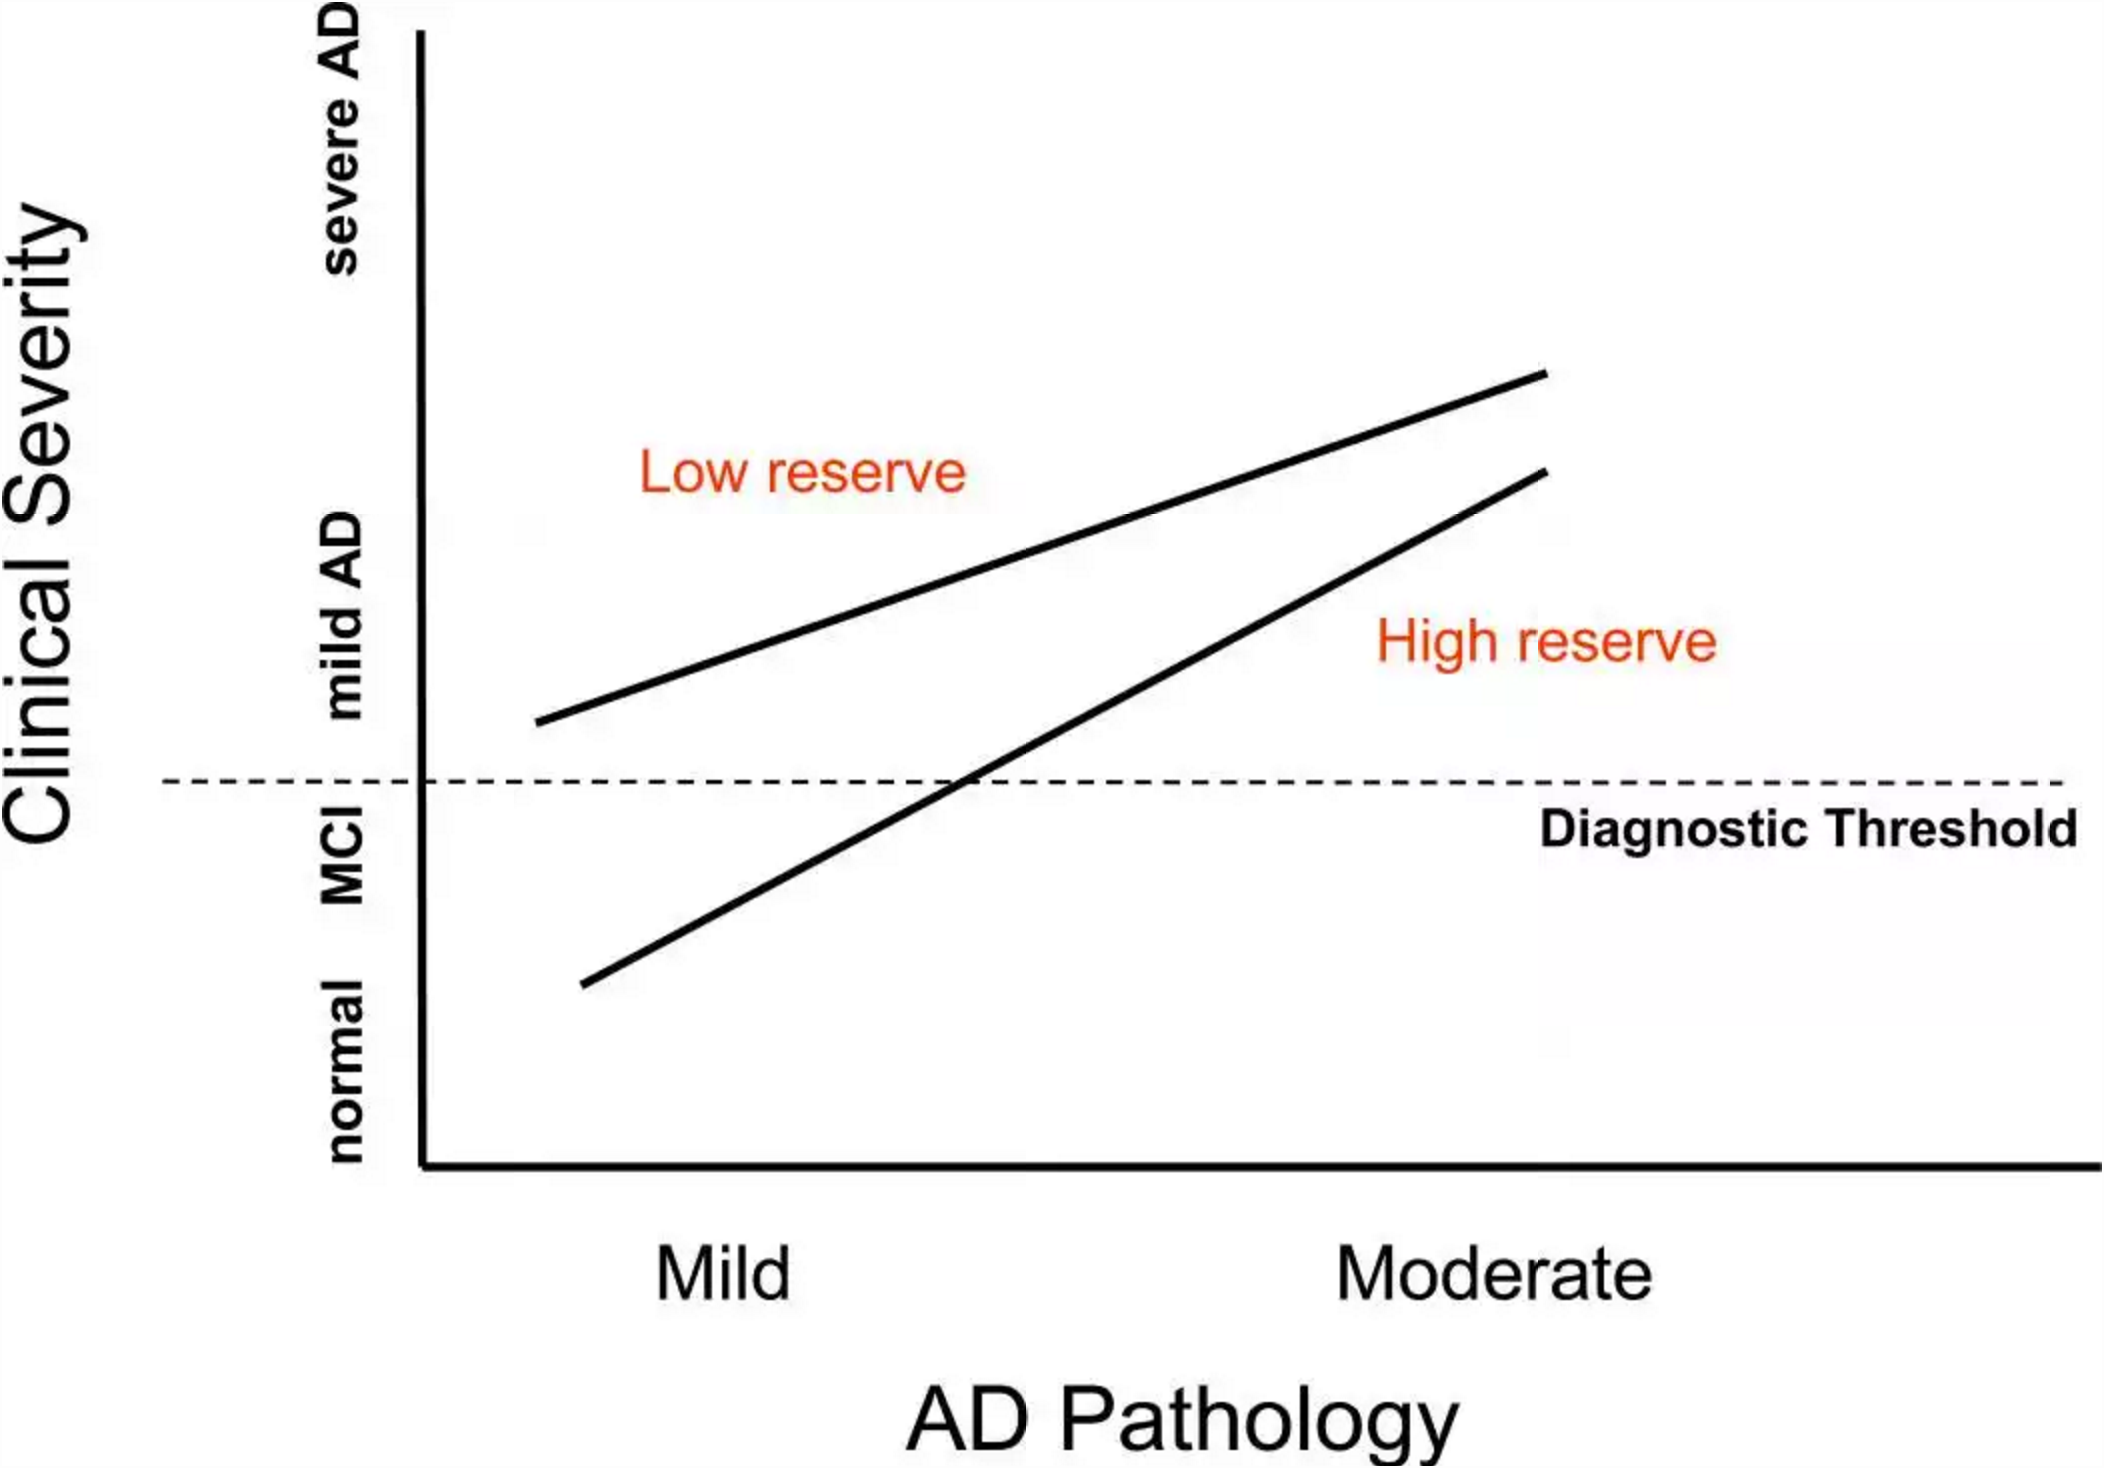
\includegraphics[scale=0.1, angle=0]{Files/literature-review/figures/lancet-neurology-adpathology}
    \caption{Theoretical effects of different levels of AD pathology, on the x-axis, and clinical severity, on the y-axis. Figure adapted from \citeauthor{Stern2012} \citeyear{Stern2012}, previously published in Lancet Neurology journal \cite{Stern2012}.}
    \label{fig: lancet-neurology-adpathology}
\end{figure}


\textbf{Head Injury.}
Those who have experienced moderate to severe head injuries have also been found to have an increased risk of developing AD.

\textbf{Air Quality.}
The quality of air also has an effect on risk. Environmental pollution, or inhalation of smoke can increase levels of free radicals in the body. Free radicals damage all cells, and their danger increases with age. This destructive nature of free radicals is believed to cause cell death in brain cells within AD \cite{AlzheimerEurope2015}.

\subsubsection{Lifestyle Risk Factors}

\textbf{Obesity.}
Having a body mass index (BMI) which is regarded as overweight or above during middle age has been found to significantly increase the risk of dementia onset in later life \cite{Profenno2010}.

\textbf{Diabetes.}
There is a link between diabetes and AD and VD. As such, diabetes brings with it an increased risk of developing dementia. AD patients are typically found to have low insulin levels \cite{Dosunmu2007}. In addition, type 2 diabetes shares the risk factor obesity, and the combination of both has been found to further compound risk \cite{Profenno2010}.

\textbf{Smoking.} As mentioned earlier in environmental risk factors, air quality is drastically reduced when smoking. Smoking is known to increase the risk of many diseases, including dementia through vascular mechanisms.

\textbf{Blood pressure.}
Non-optimal blood pressure (high/low) can also have an effect on the risk of developing dementia \cite{Qiu2005}.

\textbf{Cholesterol.}
Not all cholesterol is created equal. HDL (High-density lipoprotein) is often regarded as ``healthy cholesterol''. Conversely, high levels of LDL cholesterol (low-density lipoprotein) increases the risk of developing both AD and VD.

\textbf{Sleep.}
Poor sleep quality and short sleep duration has been linked to an increase in dementia risk \cite{Tsapanou2015}. This may be due to beta-amyloid levels increasing, a toxic protein which builds the plaques found within AD, due to poor sleep.

\textbf{Stress and Depression.}
Stress and depression are associated with an increased risk of developing dementia\cite{Saczynski2010}. The exact mechanism is not fully understood, however, the physiological and lifestyle changes that occur with stress and depression (changes in blood pressure, sleep quality, diet) may further compound the issue\cite{Schneiderman2005, Tsapanou2015}.

\textbf{Social Interaction.}
Greater levels of social engagement are associated with lower rates of dementia \cite{Saczynski2006, Fratiglioni2000}. Relationship satisfaction is also negatively correlated with dementia risk \cite{Amieva2010}, perhaps due to increased cognitive stimulation and reduced depression \cite{Saczynski2010}.

\textbf{Heavy alcohol use.}
Alcohol has been shown in studies to have a protective effect against dementias, however, large amounts and abuse of alcohol increases the risk of dementia \cite{AlzheimerEurope2015}.

\textbf{Atherosclerosis.}
The accumulation of fats on the artery walls, often referred to as plaques, reduce the blood flow to the brain, often leading to stroke. This reduced blood flow is a cause of VD. AD also has associations with various vascular conditions \cite{Dolan2010}.

\subsubsection{Modifiable Risk Factors}
Many of the identified risk factors associated with dementia can be considered modifiable; meaning that an individual can take conscious action to change their lifestyle, behaviour and environment to mitigate their risk \cite{AlzheimersAssociation2015b}. It is, however, important to recognise that insights regarding modifiable risk factors apply to large population groups, derived from studies that show associations between a factor and a dementia outcome \cite{Baumgart2015}. As such, despite addressing and correcting all modifiable risk factors, some individuals will still acquire dementia, whereas others who do nothing will not. Still, this should not deter the effort to focus on addressing modifiable risk factors across the general population. General understanding of these risk factors by the public, like the condition itself, is low \cite{Farrow2013}. In a study performed by \cite{Farrow2013}, 123 participants were assessed via a survey regarding the aforementioned behaviours and risk factors and its relation to AD risk. The respondents had noticeably less knowledge about the role of physical activity, diet, bodyweight, and diabetes, on AD risk. The study showed that after use of an informative AD website, the participants' knowledge of AD risk factors had significantly improved at the p \textless .001 level \cite{Farrow2013}.

\subsection{Impact on Everyday life}
The impact of the disease is great, not only for the PwD, but also for those closest to them. This also includes their carers, who are often close family members. As mentioned earlier, during the progression in the early and middle stages, the PwD will require additional support for various tasks that they would otherwise be capable of.

\subsubsection{Activities of Daily Living}
ADLs are those which people can normally perform without requiring additional assistance. ADLs include eating, dressing, using the toilet, continence and maintaining personal hygiene (e.g. showering and brushing teeth). During the progression of dementia completion of these ADLs becomes affected, and eventually require assistance. Often before these basic ADLs are affected, a PwD will require additional assistance with the more cognitively demanding Instrumental ADLs (IADLS). IADLS are defined as activities that are not essential for fundamental functioning, however, enable a person to live independently \cite{Bookman2007}. Examples of IADLs include preparing meals, medication management, shopping and money management.
The monitoring of these ADL/IADLs have become an important task to various health care providers \cite{Philipose2004}. By monitoring someone's performance when completing an ADL, it is possible to establish a measure of their health and cognitive well-being. If this measure begins to decline, it is an indication that some intervention may be required and the person's health and care requirements may need to be re-evaluated. Many caregiving and nursing homes record and report their patients' ADLs.
This is typically performed by the caregivers themselves, however, it has been found to be error prone, time consuming and is generally considered invasive by those being monitored \cite{McDonald2001}.

\subsubsection{Medication Management}
Medication management requires many forms of cognitive acuity, such as memory, concentration and future planning. For this reason many people require some form of reminder and scheduling assistance to help them to take their prescribed medication at the right time. The need for a reminder is even more prevalent in those with dementia, who are often prescribed complex drug regimens while also experiencing a decline in their physical and cognitive abilities \cite{Elliott2009}.
Without the use of reminders, adherence rates in the elderly would certainly decline. Adherence to prescribed medication regimens for PwD are important for a number of reasons, not limited to the sub-optimal efficacy of the treatment, however, also financially for the PwD or their family. Studies focusing on adherence rates for chronic conditions found average adherence rates ranging from 43\% - 78\% \cite{Claxton2001, Cramer2003}. Adherence rates for PwD are varied, with those living in full time care having very high rates of adherence, and those living independently having lower rates \cite{Campbell2012a}.  Successful interventions suggest that frequent reminders for PwD can improve adherence, particularly when human communication is used \cite{Campbell2012a}.

\subsubsection{Independent Living}
To live independently, free from the care of others requires autonomy and the ability to act upon decisions safely. Unfortunately, PwD often become a risk to themselves and others due to poor judgement, confusion and forgetfulness. There are many instances in which PwD have reported behaviours which placed them and others at risk \cite{Sandberg2015}, such as causing a fire by leaving a cooking appliance on. As such, assessment of independence is commonplace when caring for someone with dementia \cite{Sandberg2015, GILMOUR2003}. The benefits of residing in a care home are 24/7 access to safe and qualified care and medical staff who ensure ADLs are performed, medications are taken, and provide physical and emotional support. Despite this, 85\% of people would prefer to live at home if diagnosed with dementia \cite{AlzheimersSociety2014}. This desire to remain at home, in familiar surroundings, may be a valid one, considering that 50\% of those admitted to residential care die within 3 years, with almost one third needing palliative care within 1 year \cite{Hjaltadottir2011}. Because of this, many individuals (typically relatives of the PwD) opt to become informal carers, providing regular unpaid care and support.

\subsubsection{Care for PwD}
The role of a carer entails many tasks, and the PwD's wellbeing is their primary objective. Over time, as the condition deteriorates, PwD will become increasingly dependent on their carers, and informal carers often find themselves overwhelmed, ultimately suffering from depression and stress themselves \cite{Mahoney2005}. A day filled with numerous tasks: monitoring the PwD ensuring they do not wander, scheduling and preparing meals, arranging appointments, administering medicines, performing household tasks, and managing emotional and physical outbursts. Whilst a one-to-one care model seems apt for such an involved scenario, a current examination of care standards and staffing ratios showed the worst ratio observed was a 1:64 patient:carer ratio, whilst the best observed was a 1:5 ratio \cite{Harrington2012}. With such a stretched healthcare provisioning model, the standards of care in most countries (except Norway and Sweden) were found to be lower than the levels recommended by experts \cite{Harrington2012}.

\subsection{Technology in Dementia Research}
From analysing the pathology, symptoms, risk factors, management, and quality of care experienced by those with dementia it is apparent that the condition is complex and multifaceted. As such solutions to the issues it causes cannot be found from clinical research alone. Technology-based research within dementia has been a focal research area over the past 10 years. Initially, much effort was spent understanding where available technology could assist the condition, and initial symptomatic treatment solutions were developed, such as basic reminder systems \cite{Hersh1994, Wilson1997, Morris2003}, physical disability assistance \cite{Nugent2008b} and home-based systems aiming to improve independence and safety in the home \cite{Orpwood2005,Nugent2008b}. As time progressed and funding opportunities grew, technology solutions became more elaborate, aiming to tackle multiple issues with a single solution \cite{Zhang2008,Orpwood2005,Cook2007,Nugent2011}. During this period, smart-home technologies, which make use of embedded sensors, were proposed as a suitable and sustainable solutions for monitoring a PwD in their home. These complex solutions, once deployed, initially struggled to handle the complexity of human behaviours, especially those observed in a PwD, who can behave unpredictably. Smart-home solutions have since improved somewhat through further research, and their use in dementia care is still an active research area \cite{Amiribesheli2015,Wilson2015a}. Much of the research performed on technology in dementia has been focused on the treatment of the condition; relieving symptoms, easing burden, increasing safety and improving care provisioning \cite{xhafa2015, Gillespie2012, Cahill2008}. Recently, it has become apparent that there may be an opportunity for technology in the prevention effort against the condition. \citeauthor{Mangialasche2012} noted that a promising strategy for preventing dementia would be to implement an intervention program that takes into consideration the multifactorial nature of dementia \cite{Mangialasche2012}. Technology may therefore the key to deliver such an intervention to the masses through its ubiquitous reach.

\section{Treatment: Current State-of-the-Art} \label{section: treatment-stateoftheart}
As previously discussed, the use of technology in the dementia epidemic may be categorised into the areas of treatment and prevention. Treatment refers to the use of the technology to alleviate issues caused by dementia, and also symptomatic aid, rather than a curative effect.
This Section will discuss the state of the art in this area, highlighting the benefits, current limitations, and the opportunities for improvement.

\subsection{Smart-homes}
Smart-homes and their supporting software systems are the cutting edge of treatment solutions for dementia. Previously only accessible to those in the research domain, smart-home technologies are slowly being refined and developed for the consumer market. These include automated products that can increase home security, control heating, lighting, and detect spoiling food in a smart fridge \cite{Hoy2015, IControlStateofArt2015}. Many of these consumer grade products do not meet the additional demands that a PwD creates. As such, smart-home systems that specifically address these specific needs are very much still within the research domain. Much focus has been placed on the monitoring and assistance of ADLs, using a variety of sensors and machine learning algorithms \cite{Cook2007, Cook2012, Hoey2007, Hoey2010, Chen2012}. The detection of harmful incidents, such as unexpected falls in the elderly, is also a prominent research area in the field of smart-home applications \cite{Chaquet2013,Yang2010}. Other uses include the detection and subsequent redirection of pacing, a common occurrence in which PwD become restless and walks in an attempt to perform various purposeless activities \cite{Nugent2011}.

\subsubsection{Complexity}
Despite the numerous potential uses many of these solutions fall victim to the sheer complexity of human behaviour, along with interoperability and scalability issues \cite{Cook2007, Tang2010, Lim2008}. Along with this, a unified vision and understanding of who `smart-home' users are, and how they might use the technology is missing from ``a field being overwhelmingly pushed by technology developers'' \cite{Wilson2015a}. In addition, many of the algorithms and proposed solutions, despite providing promising accuracies in technical tests, have not been efficiently trialled in valid scenarios with PwD, and as such their true efficacy has not been assessed \cite{Dawson2015, Lyons2015}.

\textbf{Benefits.}
Reduce caregiver burden; Increased PwD safety; Assistance with ADLs; Remain at home longer.

\textbf{Limitations.}
System complexity; Cost of installation and maintenance; Scalability issues; Not Readily Available; No evidence-based RCTs.

\subsection{Cognitive Aids}
Failing memory and ability to plan is undoubtably a prominent feature of dementia. As such, there is an opportunity to improve memory and planning using cognitive aids, such as reminders and scheduling tools. Reminder systems for the cognitively impaired have evolved with the technology, and now range from the simpler time-specific reminders to complex context-aware reminder systems, incorporating numerous environmental sensors \cite{Hersh1994, Zhang2008, Zhou2012}. Reminder systems to aid scheduling can be classified into 4 main groups, based on the type of information used to issue the reminder: (1) time-based, (2) location-based, (3) activity-based and (4) hybrid reminder systems \cite{Seelye2012, Hartin2014-IWAAL}.

\subsubsection{Time-based}
For PwD time-based scheduling is the most rudimentary and the most commonly implemented. NeuroPage \cite{Hersh1994, Wilson1997} is one such example. It was designed to be used by persons with memory impairments as a result of brain injury, however, could also be used by those with progressive conditions, such as dementia. Time-based reminders whilst extremely reliable face the issue of delivering reminders during inconvenient situations, such as when the user is eating, working or in a different location from the reminding device. These types of situations can cause a person to experience stress and increased frustration, given that they feel obliged to address the alerts \cite{Mark2008}, which can only be exacerbated with dementia symptoms.
Consequently, location and activity based reminders aim to observe and avoid these types of situations, opting for a model which prioritises the current observed activity or location for the delivery of a reminder, rather than the time.

\subsubsection{Location-based}
Location-based reminders use an individuals observed location to influence the delivery of a reminder. The use of location information has taken many forms both inside the home, and outside. \citeauthor{Marmasse2000} pioneered the use of GPS to deliver location-based messages to a mobile device when the device was in proximity to a pre-programmed target, e.g., a shopping list sent when near a store \cite{Marmasse2000}.
Whilst building upon simple time-based solutions, the limitations of these systems are that they are typically restricted to one format of prompt (e.g., text or voice instructions), do not consider other available contexts (e.g., activities, time) and as such are incapable of avoiding delivery during inappropriate times, or during complex activities (e.g., driving at night) \cite{Seelye2012}. \citeauthor{Tu2013} addressed some of these issues in their iReminder solution, which was capable of predicting a user’s future location based on previous routes and delivered a location specific reminder before they arrived, thus potentially minimising inappropriately timed messages \cite{Tu2013}. These models and techniques, whilst originally based outside the home, have been applied to the technology and dementia paradigm. The introduction of GPS in dementia care took the form of geofencing \cite{Wang2015}, enabling carers to be alerted when a PwD left a pre-set boundary, such as wandering from their home in the middle of the night. Inside the home, however, it is very difficult to track the PwD's movements, due to minimal, or nonexistent GPS signal. As such other methods have been developed to track the current location of people within the home, including pressure sensors, infrared and Wi-Fi signal strength \cite{Chen2012}. Again, reminder solutions for PwD in the home, using location as their primary context also experience the same limitations, with the additional complexity of PwD behaviour \cite{Grunerbl2011,Lin2014a}.

\subsubsection{Activity-based}
Activity-based reminders offer a potential solution to the complexity of a PwD's unpredictable daily schedule. Rather than prescribe a one-size-fits all time-based reminder system, activity-based systems aim to learn or deliver pre-programmed reminders when certain activities are detected. For example, these proposed systems could remind a PwD to turn off the oven or take specific medications once a meal has been prepared, increasing safety and medication compliance.
Activity-based reminders rely heavily on the field of pervasive computing and activity recognition, a field which aims to detect people's activities and behaviours. Home-based activity recognition typically makes use of an array of sensor modalities, which include contact, pressure and heat sensors, infrared movement detectors and varying formats of video \cite{Chen2012b}. Accounting for these varying types of data increases the complexity of the system, however, when performed correctly, can also increase the accuracy of the activity classification. Within the dementia care paradigm, activity recognition is proposed to monitor ADLs, assess their progression and provide assistance or prompts (reminders) when needed. Systems that use one sensor modality are much more scalable, however, are somewhat limited to the classification of actions, e.g., opening a cupboard door, rather than the overarching activity \cite{Chen2012b, Patterson2015}. If a system is to understand why the cupboard door has been opened, then additional input is required to increase the systems understanding \cite{Chen2012}. As such, the current approach to activity-based reminders require a number of sensor modalities and accompanying machine learning models to infer activities accurately. Autominder \cite{Pollack2003} is an activity-based reminder system that uses artificial intelligence techniques and quantitative temporal Bayesian networks to observe and reason about ADLs using a robot, which have been performed to develop a model of an elder’s typical daily plan. The system maintains and uses this model to schedule future reminders, however, once a given schedule is learned, it cannot be altered.
The limitations of these approaches are shared with the smart-homes described earlier, in that they are expensive to purchase, install and maintain, suffer scalability issues \cite{Wilson2015a} and any sensor failure greatly impacts the systems visibility and thus reliability \cite{Ye2015}.

\subsubsection{Hybrid}
Recognising the insight that each context brings, hybrid solutions aim to utilise all available contexts, optimising accuracy by selecting the most appropriate for any given situation. Such a goal is admirable, however, highly complex. Many frameworks and architectures have been proposed, however, suffer from the same issues; scalability, complexity and variability. Whilst rules may be used to discern which contextual input is more appropriate in each scenario, the list of scenarios can be infinite, and even so, these rules will vary from one PwD to the next. The COGKNOW project  proposed a complex context-aware system for persons with mild dementia \cite{Zhang2008}. The architecture incorporated time, location and user activity as contexts, along with the time that the to-be-prompted activity was typically performed. The full feature set of the system was, however, not realised upon the project’s close. iConAwa, proposed by \citeauthor{Ylmaz2012}, was another intelligent context-aware system proposal which aimed to provide smartphone users with context-aware information and services \cite{Ylmaz2012}. The paper presented a set of novel case studies, in which a number of users with a number of interests received prompts related to services which may be of interest. The system used location, time, network connectivity and user preferences as contexts.  The entire system was based upon a complex, user maintained, rule-based ontology, encoded in OWL (Web Ontology Language). Despite a novel and promising framework, the solution was never developed, deployed or evaluated.

\subsection{Reducing Complexity}
Much of the research in this area has been driven by the technology sector, forsaking patient needs for technical complexity.
The need for a PwD is to be given the appropriate reminder, at the appropriate time, in a manner they can comprehend. This need has become obscured over time, and has slipped into an approach of constructing the most elaborate systems, with each iteration becoming more complex and technologically novel, albeit lacking any real merit for the end-user. None of the aforementioned studies or systems considered how delivery of the reminder may interrupt the user, nor did they alter the delivery based on existing evidence, extracted from past acknowledgment rates \cite{Hartin2014-WAGER}.

\subsection{Areas for Contribution}
There is therefore the opportunity to reduce complexity and increase efficacy in reminders for PwD. Chapter \ref{chapter: treatment-framework} addresses these areas using a simpler approach; a smartphone app to monitor acknowledgement rates to temporal-based reminders, learning usage patterns through the embedded sensors, with the aim of improving reminder delivery and adherence for each individual. Chapter \ref{chapter: treatment-framework} details the development of the reminding solution and preliminary testing with a healthy cohort. Chapter \ref{chapter: treatment-framework} details the results from usage of the app by over 30 PwD in a 12 month trial. Sensor based reminding is also then optimised for this particular cohort and future improvements are discussed.

\section{Prevention: Current State-of-the-Art}
To date, technology's opportunities in the dementia epidemic has almost exclusively been in the area of treatment. Recently, prevention of the condition has been identified as a priority. With the advent of wearable technologies and increasing smartphone usage and capabilities, a new opportunity has arisen to use these tools to focus on the prevention of the disease.
This Section will discuss the shift of focus to prevention, the current state of public health campaigns and technology's role, and also the state of the art in smartphone and wearables.

\subsection{Adjusting the focus to prevention}
During the course of study into dementias, and attempts to develop a cure, various risk factors have been discovered and extensively studied \cite{Baumgart2015}. This work resulted in sentiments which claimed that whilst dementia was not curable, the clinical evidence suggested that it was preventable in many cases \cite{DelaTorre2010,Willis2013}. The AD research community responded by addressing government bodies at the G8 summit in 2013, requesting that AD prevention be placed as a major health aim, and calling for others to further study the risk factors associated with the condition \cite{Smith2014}. Advances since have suggested that the management of modifiable risk factors may hold the key to dementia prevention, especially for AD and VD \cite{Solomon2014, Lovden2013}. Many of the risk factors identified can be addressed by simply improving ones general health;improving diet, increasing exercise, improving sleep quality and reducing stress. Since the development of public health in classical Greece, improving the general health of the population has been a key objective \cite{Ozonoff1994}. In the modern era, many public health campaigns have aimed to improve the general health of the population to mitigate future risk and treatment costs of specific diseases, such as heart disease, stroke, diabetes and obesity \cite{Labarthe2014, CentersforDiseaseControlandPrevention2015}.

 \subsection{Public Health Campaigns}
Whilst the need for a public health campaign for dementia risk is obvious \cite{cook2014public}, the most effective delivery method is not. In recent years, ICT has been increasingly used to extend the delivery of public health campaigns \cite{Mirarchi2015}, and in some cases, used as the primary method of delivery \cite{Hattink2015}. These ICT enabled campaigns typically utilise the world wide web as their platform for distribution. Often they may take the form of a static webpage which displays information about a condition, current prevalence, generalised risk statistics, and various steps to improve outcomes \cite{AlzheimersAssociation2015a}. This model is effective for a number of reasons, with accessibility being the primary advantage over classical approaches. Information is generalised and presented in a clear and concise manner, it is accessible at any time, and on a variety of internet ready devices, however, it is up to the user to understand the information and enact upon any recommendations provided, which is where the efficacy of this approach begins to experience its limitations. Whilst the information is accessible, it is generalised and non-specific to the reader which can lead to confusion and non-adoption of the recommendations \cite{lerouge2014challenges, Tones1994}. It has also been found that may of these websites suffer from poor readability \cite{RisoldiCochrane2012}, which may result in sub-optimal learning outcomes. The authors of this research suggest that additional effort be made to ensure that all health information communicated is easy to read and understand \cite{RisoldiCochrane2012}.

\subsubsection{Increasing Interactivity}
One possible approach to improve the understanding and subsequent adoption of any public health recommendation is to improve the interactivity of the content. Increasing interactivity online has been shown to improve learning outcomes, especially if the content is perceived as being useful \cite{Oh2015, Wei2015}. Evolving from the static webpage model described earlier, an education portal provides a structured learning approach, using teaching modules to guide progression through content, and often utilise interactive tools such as glossaries, pop-quizzes and games, to help boost understanding \cite{Hattink2015}. This portal approach has been successfully applied in the past to educate informal carers of PwD, from various levels of education, about the condition and provide advanced caregiving and coping techniques \cite{Hattink2015}.
Whilst often more interactive than static information pages, the education portal solution can add unwanted complexity for the user, requiring an active internet connection to use and typically requiring account registration to use the platform.
Smartphone apps provide an opportune platform to deliver educational information with an interactive component. Touch interfaces have been found to be more engaging for learning purposes \cite{Jones2006}, and due to user-design guidelines provided by Apple and Google \cite{AppleNotifications2015,GoogleAndroid2015}, the quality of interactive apps is ever increasing. It has become the status-quo to provide highly interactive features in the most basic of apps. Nevertheless, the availability of apps or mobile ready content has been found to be considerably low within public health. One study of 55 American health websites found that only 22\% (n=12) were considered mobile ready, of which only one-third had better or similar readability to their traditional website counterparts \cite{Cunningham2015}.

\subsubsection{Health Campaign Apps}
With 2015 being the year in which smartphones surpassed personal computers as the most popular method to access the web, it is suggested that public health campaigns recognise this shift and adapt accordingly \cite{Cunningham2015}. Anticipating this shift, the US Centers for Disease Control and Prevention (CDC) were one of the biggest public health authorities to 'go mobile' in 2013, by launching a free public health app service on the Google Play store and Apple App store \cite{CentersforDiseaseControlandPrevention2013}. This prompted a surge in the development of public health apps, published from various leading authorities including the United Nations \cite{UnitedNations2015}. These public health apps include helpful tools to schedule vaccines \cite{CentersforDiseaseControlandPrevention2015b}, apps which encourage swimming as a form of exercise \cite{CentersforDiseaseControlandPrevention2015a}, information on diet when travelling to avoid travellers’ diarrhoea \cite{CentersforDiseaseControlandPrevention2015c}, and even an app which advises on the correct angle of a ladder to minimise the risk of falling injuries \cite{NationalInstituteforOccupationalSafetyandHealthDivisionofSafetyResearch2014}. Whilst these apps are from credible sources and contain valid information, they are not end-to-end solutions designed to measure any change at an individual level, such as the adoption of suggested behaviours or monitoring health metrics.
The technology to perform these tasks does exist and comes in a variety of forms. There is therefore, an opportunity to advance these public health campaigns, and enable them to engage with the population more effectively at an individual level.

\subsection{Everyday mHealth}
The use of technology to monitor everyday health is a thriving area, both for researchers and consumers alike. Currently, there are over 165,000 health and fitness smartphone apps available, and over 280 wearable devices aiming to seamlessly monitor health \cite{IMSmHealth2015}. Many of these apps and devices can be used for the purposes of mHealth (Mobile Health), an area which advocates the use of mobile (including wearable) devices to support the practice of medicine and public health \cite{Adibi2015}.

\subsubsection{Smartphones and app}
mHealth apps are quickly becoming the go-to tools for condition monitoring, providing a convenient and cost effective way for individuals to measure many vital signs, including pulse rate \cite{Led2015, Baig2013}, blood-pressure \cite{Moser2015}, blood-oxygen \cite{Led2015, Moser2015} and also blood glucose \cite{Moser2015}. In addition to these cardiovascular measurements, the smartphones camera may also be used to perform eye \cite{Maamari2014}, ear \cite{Rappaport2015}, and dermatological examinations \cite{Kassianos2015}. Physicians are increasingly using these validated applications in their practices \cite{Topol2012}, however, not all mHealth apps are created equal. The number of health and wellness apps available has more than doubled since 2013, yet many have no scientific evidence base. Figure \ref{fig: imshealth-mhealthapps} shows the type distribution of mHealth apps currently available  in the app marketplace.

\begin{figure}[h]
    \centering
    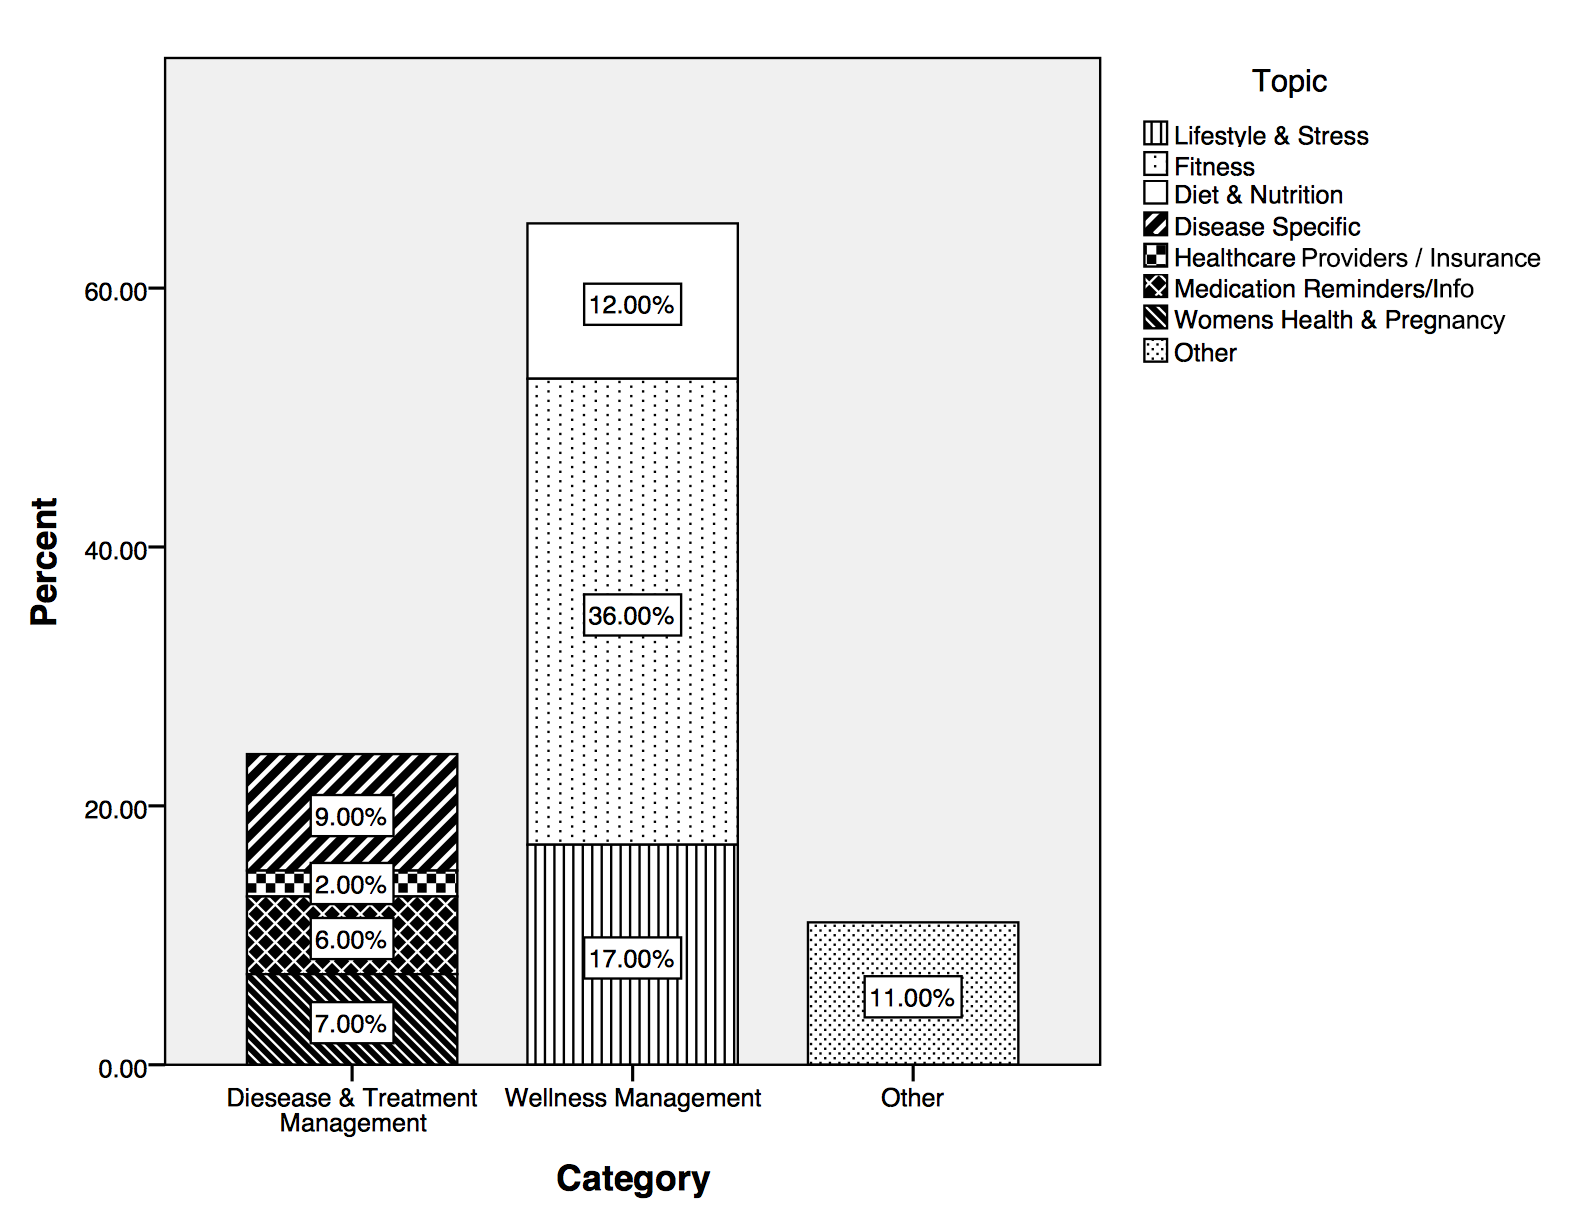
\includegraphics[scale=0.25, angle=0]{Files/literature-review/figures/imshealth-mhealthapps}
    \caption{Categories of mHealth apps available on iOS and android app stores in 2015; data adapted from \cite{IMSmHealth2015}.}
    \label{fig: imshealth-mhealthapps}
\end{figure}

The majority of these apps are categorised as ``wellness management'' apps, of which fitness apps, contribute the greatest to the overall number. Recent articles published in the British Medical Journal (BMJ) \cite{Husain2015} and the Journal of the American Medical Association (JAMA) \cite{Kuehn2015} raised concerns due to the lack of process when publishing a healthcare app on app marketplaces. As a result the vast majority of ``health apps'' have not been assessed by any credible bodies for the information or methodologies that they disseminate. This fact alone stands to cripple the widespread adoption of mHealth solutions due to providers, and consumers, views regarding lack of evidence and credibility \cite{IMSmHealth2015}. There is therefore an opportunity for technology researchers to develop healthcare apps, whose methods are underpinned by clinical literature and evaluated scientifically, to demonstrate the potential impact of widespread adoption.

\subsection{Wearables}
Wearable devices have seen considerable adoption in recent years, driven by demand in the fitness market. The majority of these devices (\textgreater50\%) have been designed to be worn on the wrist, around a quarter are designed to be worn around the chest, and approximately a fifth are designed to worn in the pocket, shoe or purse, as shown in Figure \ref{fig: imshealth-wearableposition} \cite{IMSmHealth2015}. Wearables, despite being standalone devices, often require a smartphone app to sync, extract, and analyse collected information.

\begin{figure}[h]
    \centering
    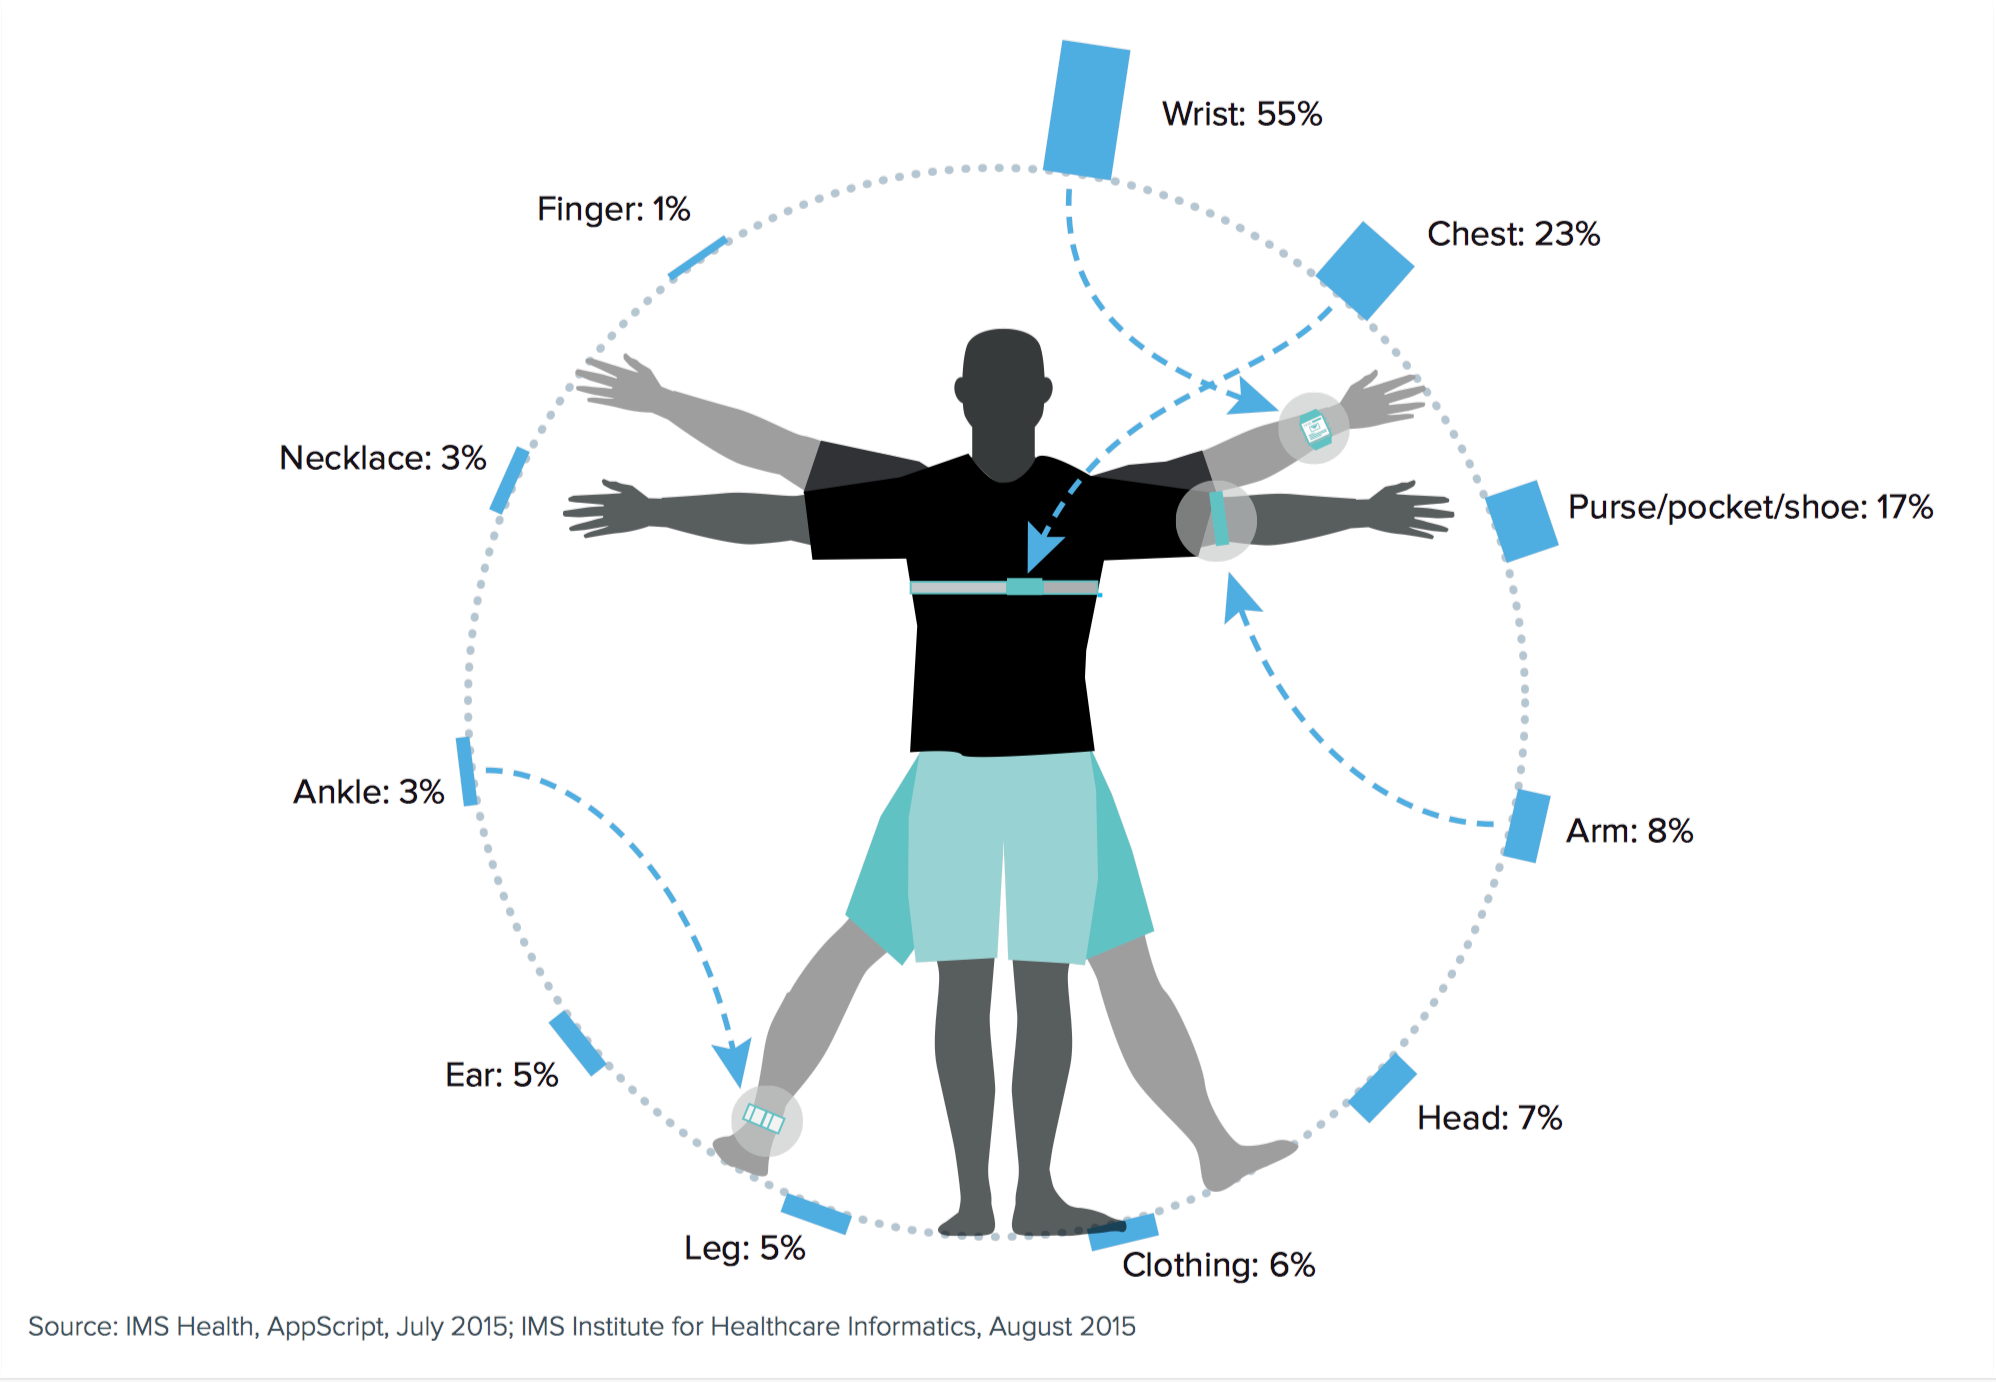
\includegraphics[scale=0.2, angle=0]{Files/literature-review/figures/imshealth-wearableposition}
    \caption{Placement of portable and wearable devices as found by \citeauthor{IMSmHealth2015}. \textit{Source: IMS Health, AppScript, July 2015; IMS Institute For Healthcare Informatics, August 2015} \cite{IMSmHealth2015}.}
    \label{fig: imshealth-wearableposition}
\end{figure}

Similar to the type distribution of mHealth apps, wearable devices targeting general fitness accounted for the largest number of wearable devices in an analysis study by \cite{IMSmHealth2015}. This is presented in Figure \ref{fig: imshealth-devices}. Unlike mHealth apps, however, there are greater barriers to market entry, notably the mass production of hardware, marketing, and research and development. As a result, the standards of available solutions are high, with many device's accuracy claims being independently evaluated and validated by academics \cite{Ferguson2015}.

\begin{figure}[h]
    \centering
    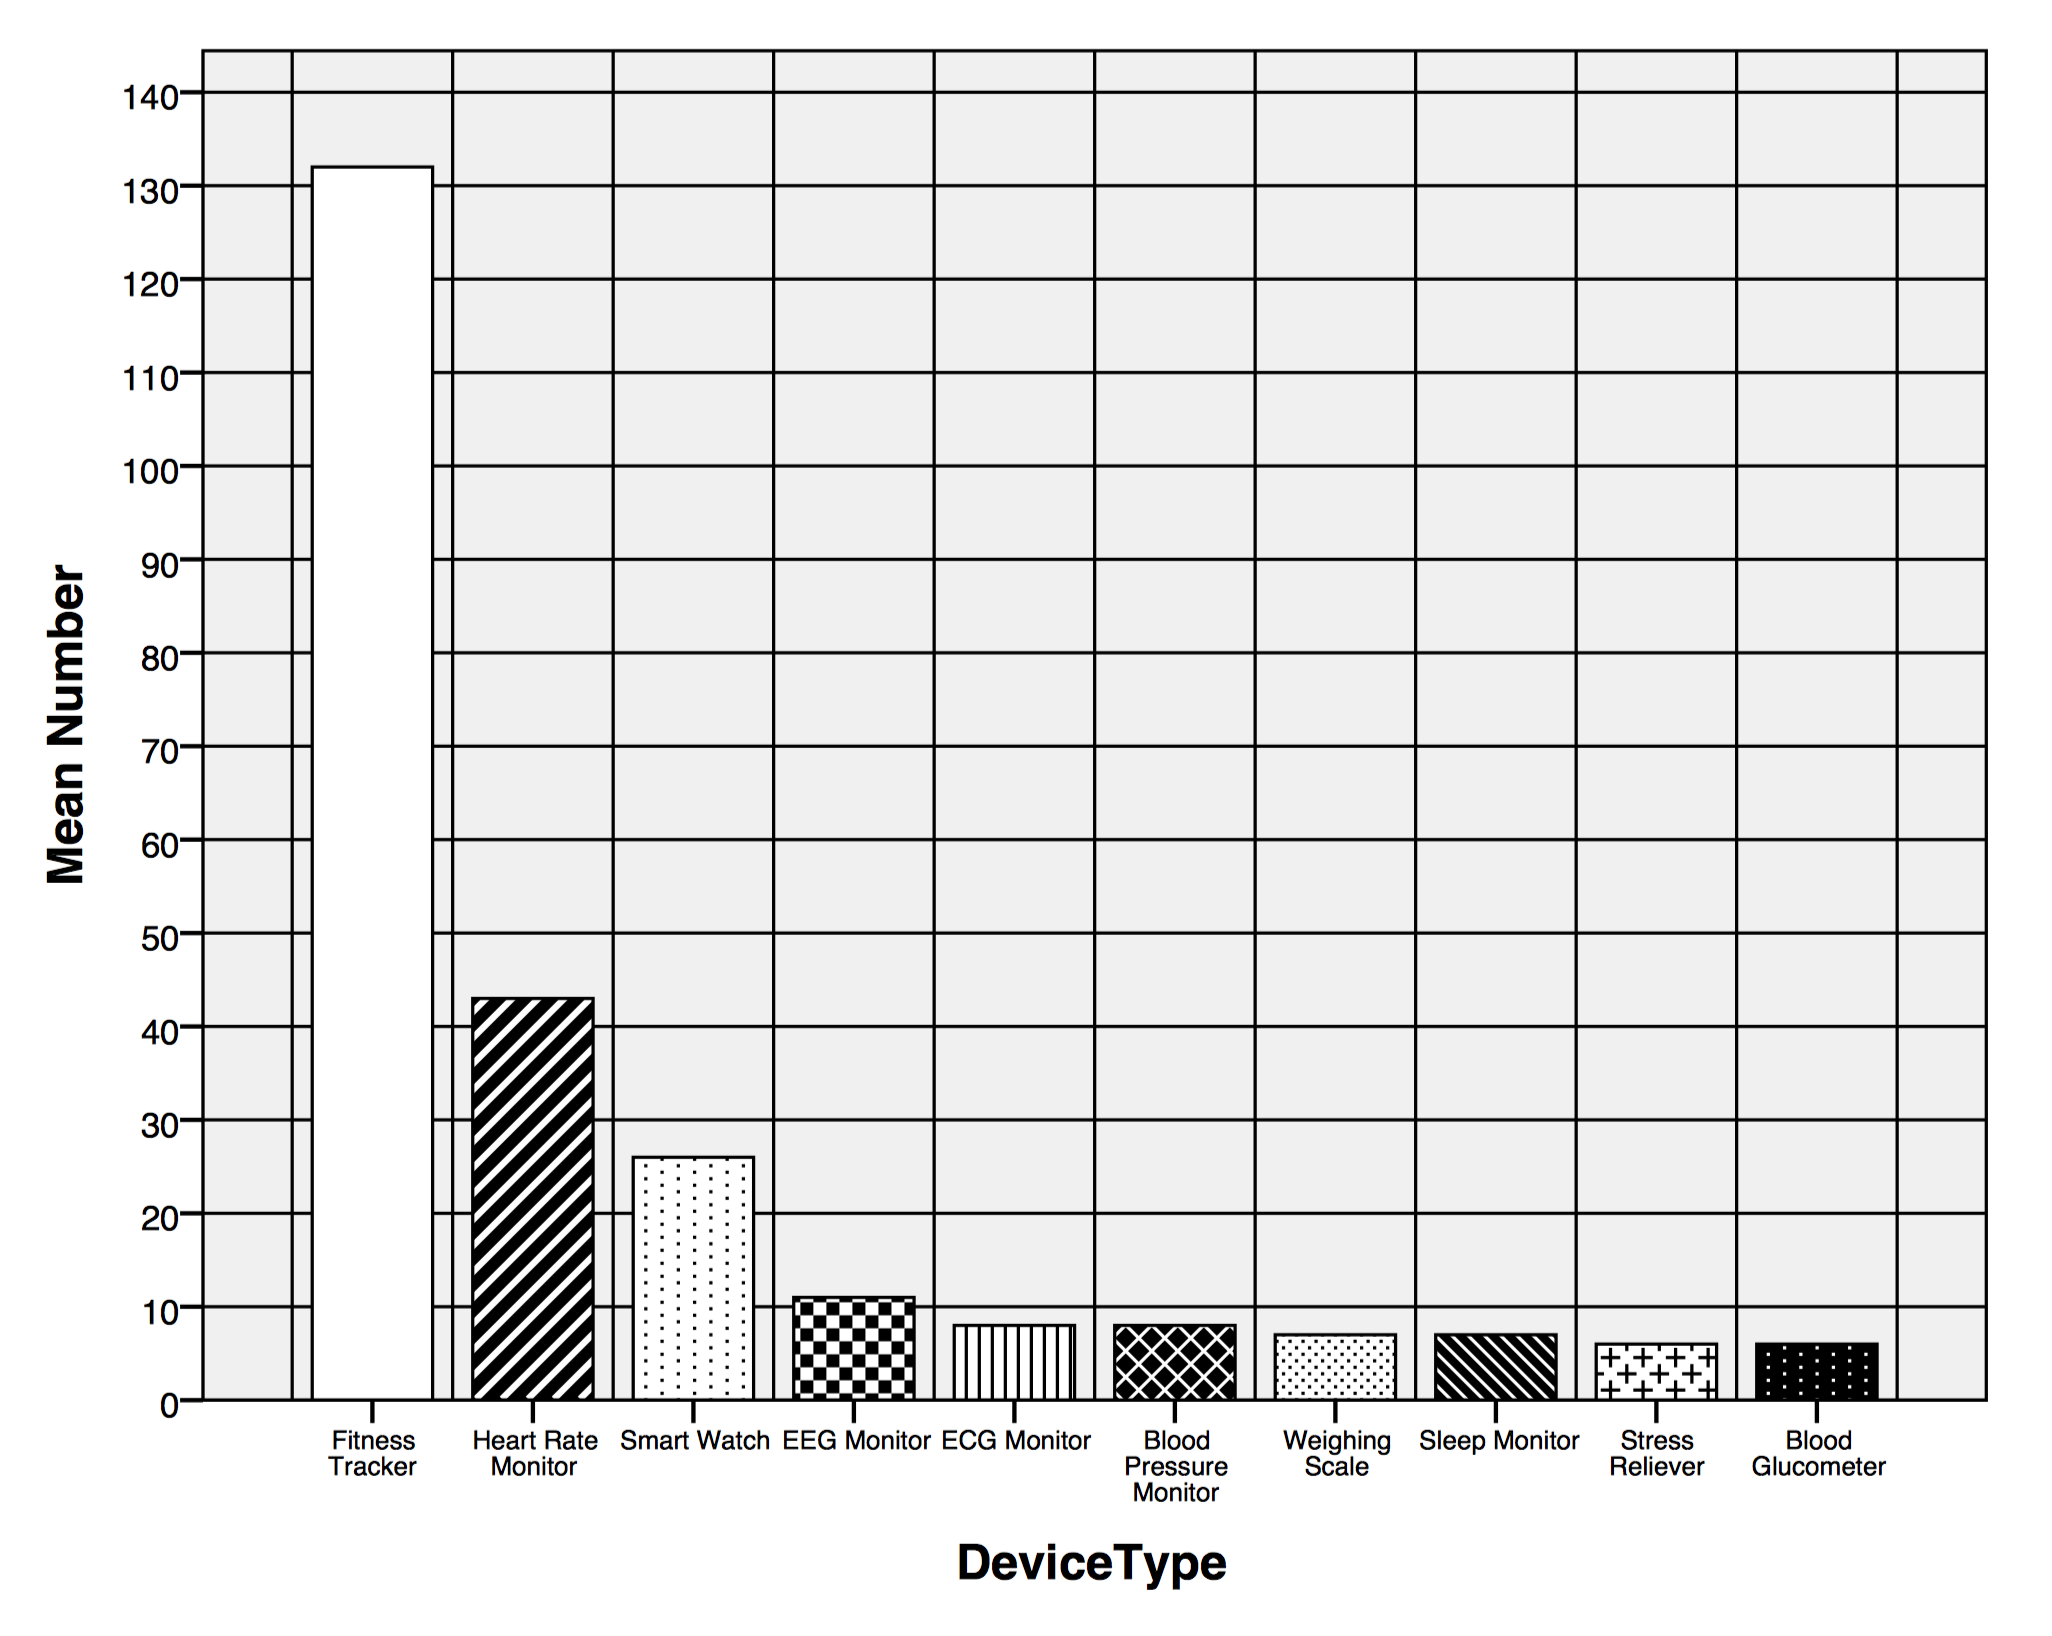
\includegraphics[scale=0.35, angle=0]{Files/literature-review/figures/imshealth-devices}
    \caption{Availability and type of dedicated health and fitness devices; graph adapted from data in \cite{IMSmHealth2015}.}
    \label{fig: imshealth-devices}
\end{figure}

\subsection{Health Monitoring Functions}
Many functions provided by wearable devices and smartphone apps are shared, due to shared hardware, yet each platform can be more suitable than the other in specific scenarios. For the purpose of overall health monitoring, the functions of physical activity monitoring, vital signs monitoring, diet management, sleep assessment and coaching are investigated further.

\subsubsection{Physical Activity}
Physical activity can be monitored by smartphones and wearables in a variety of ways, including the use of embedded sensors. The most commonly implemented feature across all devices is the step counter.

\textbf{Step-Counter.}
Accelerometers and gyroscopes embedded in smartphones and wearables can be used to detect stepping patterns, enabling the devices to be used as pedometers. Originally implemented by independent developers, step-counters have become a standard feature of smartphone devices, with native functions built into the operating systems of both iOS and Android \cite{Orr2015}. Step-count can be a useful measure of overall physical activity performed in a set period (i.e. number of steps per day). As such, it is used as a primary measure in most wearable devices, with daily step count goals established via software. Many evaluations of accuracy have been performed for smartphone and wearable pedometers \cite{Cleland2012, Cleland2013, Yang2010}, including comparative studies \cite{El-Amrawy2015}. Despite similar accuracies, it is often the case in real-world scenarios that smartphones are not present on a person 24/7, and as a result will miss a number of instances.

\textbf{GPS.}
Using GPS it is possible to increase the accuracy and granularity of physical activity data. Especially useful for monitoring distance sports such as running and cycling, it is possible to track the location history of an individual, distance travelled, establish speed, and estimate calorie expenditure \cite{Zhan2012, BUTTE2012}. This gives a much deeper insight into the physical activity performance, however, but for the purpose of general physical activity GPS is superfluous and will cause excessive battery drain in both smartphones and wearables \cite{BUTTE2012}. In addition, loss of a GPS signal when travelling indoors will result in missing or inaccurate data. Due to this, it is recommended that GPS only be enabled for distance and speed specific activities.

\textbf{Self-reporting.}
There are a number of scenarios where it would be inappropriate to use wearables or a smartphone to track physical activity, e.g. swimming and contact sports. In these cases many solutions allow for self-reporting of activity. Using existing and validated data, it is possible to estimate calorie expenditure for a number of activities, based upon the users age, height and weight, the physical activity performed and the duration and intensity \cite{Black1996}. Self-reporting may also be used to amend and correct activity labels classified from a smartphone or wearable. e.g. in some cases, cycling at a slow pace can be misinterpreted as running in various activity recognition models, resulting in incorrect calorie expenditure \cite{Ferguson2015}.

\subsubsection{Vital Signs}
Originally developed to extend primary and ambulatory care \cite{HOLTER1949}, portable heart rate (HR) monitoring has permeated into the consumer market through the demand of fitness enthusiasts. A variety of methods exist to establish HR, however, the most commonly implemented is via the use of photoplethysmography (PPG). PPG is a low-cost optical technique that uses light and a receptor to detect blood volume changes in a bed of tissue \cite{Allen2007}. In wearables the light source and sensor is often located on the back of the watch face pointed toward the skins surface, and in smartphones a combination of the phones LED flash and rear facing camera are used \cite{Asada2003}. By illuminating capillaries under the surface of the skin with the LED, small changes in luminance are detected by a sensor. These changes occur due to blood being pumped, and a measure of frequency can be established (HR). Typically a filter is applied to the signal to remove artifacts caused by motion, resulting in a smoother signal and better estimate of actual HR \cite{Chan2002}. This method of detecting heart rate, whilst convenient and non-invasive, can suffer from inaccuracies due to vigorous physical activities and incorrect placement \cite{Parak2014}, which often occur simultaneously. The method does excel, however, for 24/7 HR monitoring, providing accurate readings for resting HR, which is often used as a reliable indicator of overall cardiovascular fitness \cite{Mukhopadhyay2015, Steinhubl2015}.

\subsubsection{Sleep Monitoring}
Similar to the step-counter, onboard accelerometer and gyroscope sensors are used to detect movement occurring during sleep. With increased movement, a poor sleep quality is assumed. Some smartphone apps also include microphone decibel readings to further influence their quality assessments \cite{Calikli2014}. Sleep monitoring using a smartphone is performed by placing the smartphone on the mattress and running the monitoring software. The accuracy of this approach may be compromised if the bed is occupied by more than one person, and also requires a manual start and stop of the recording. Wrist worn wearables address these limitations, measuring only the wearers movement and automatically recording sleep \cite{VanHees2015}, however, many people, especially the elderly, find it uncomfortable to wear in bed \cite{Fisher2015}. A solution that addresses all these limitations is a fixed sensor bed, which can be placed on top of the mattress and requires no additional setup. These standalone devices are considerably more expensive and their accuracies require additional validation \cite{Ko2015}.

\subsubsection{Diet Management}
Diet plays a vital role in general health, however, its management is often tainted by poor understanding and great anxiety. Technology in diet management has been predominately used to facilitate meal logging, enabling calorie estimations. Wearable technologies do not have much input in this area, other than to act as dietary reminders to eat or rehydrate \cite{Fortmann2014}. Smartphone apps, however, provide numerous methods to help track diet and estimate calories. An existing and highly efficient method of recording diet with an app utilises the smartphone camera to scan the barcodes of food items, which retrieves nutritional information from a community maintained food information database \cite{Breton2011}. The use of a food database also greatly reduces the risk of human error when entering calorie information \cite{Turner-McGrievy2013}. The scanning method is useful in scenarios were the food is from a known source, and with a printed barcode, however, is limited for use in home-made or restaurant meals. To overcome this limitation, novel research has proposed the use of the smartphones camera, to take a picture of a meal, and estimating the calorie content using image processing techniques \cite{Villalobos2012, Pouladzadeh2014}. Regardless of the information source, the calorie information can be correlated and compared with physical activity information, which may be recorded by the same smartphone or wearable. This provides users with accurate estimates of calorie expenditure vs consumption, a helpful tool to successfully manage weight \cite{DeLany2014}.
Calories, whilst an important factor of diet management, do not provide information regarding diet quality \cite{Wirt2009}. In an 8 week trial using an mHealth diet app to help participants lose weight, researchers found that whilst participant self-monitoring and calorie reduction improved, diet quality did not \cite{Wharton2015}. The nutritional quality of diet is of paramount importance for optimal health outcomes, especially with the existing evidence. In a study involving over 424,000 participants it was found that regular consumption of high-quality foods resulted in an 11–28\% reduced risk of death due to all causes, independent of co-founders \cite{Liese2015}. It is suggested that an app aiming to reduce the risk of developing AD, and other conditions, should make dietary recommendations based upon quality first, and caloric content second.

\subsubsection{Remote Coaching}
Whilst a coach may traditionally suggest a gym instructor, the term encompasses anyone who is an expert in a specific field who instructs another individual toward a goal, thus, coaching them. Remote coaching via the internet has become a lucrative business model for many, with coaches advertising their expertise in physical fitness, relationships, stress management and healthy eating \cite{Smith2014a, rossett2005if}. Using internet-based technologies, remote coaches are capable of analysing their clients behaviours, which may be either self-reported or recorded via technologies\cite{Jimison2015,eemcs22577,kyfonidis2015future}.
In the commercial domain the validity of advice cannot be guaranteed \cite{Smith2014a}, however, research has shown the use of remote coaching to be of great value in studies wishing to remotely coach exercise and physical therapy \cite{Jimison2015,Geraedts2013,Spring2012}, healthy diet \cite{Spring2012}, and smoking cessation \cite{Sforzo2014}.
A huge advantage over physical coaching is the accessibility and availability of an online coach, providing access to encouragement and peer support when it is most needed \cite{kyfonidis2015future}. A study of 200 adults, aged 21-60 years, who were deficient in various healthy behaviours, found that the use of remote coaching could significantly positively effect behaviour change \cite{Nothwehr2013}. The investigator \citeauthor{Nothwehr2013} noted the huge potential for mobile technology to both encourage behaviour change, and to provide exceptionally rich data for researchers studying the behaviour change process \cite{Nothwehr2013}.

\subsection{Areas for Contribution}
Despite the number of mHealth apps doubling since 2013, innovation has been relatively static. Apps and wearables hold the power to influence and ultimately change behaviours, yet for the most part this ability has remained unharnessed.
There is therefore the opportunity to exploit the effectiveness of this technology and fortify it with the input of behavioural psychology, to ultimately innovate the method in which public health and disease prevention is approached.

Chapter \ref{chapter: prevention-framework} describes the development of a mobile health intervention framework, which harnesses existing technologies to provide support for behaviour change to mitigate future risk of various chronic conditions. The framework is then applied to AD, and an app is developed. The resultant app is then evaluated in Chapter \ref{chapter: prevention-evaluation} by a number of domain experts and compared to existing healthcare apps. Content analysis of the app, along with existing apps, is also performed, from which a number of recommendations for future development are established. Chapter \ref{chapter: prevention-rctresults} details the results of a randomised control trial, in which over 100 healthy middle-aged persons used the app for a period of 6-months with the intention of inciting positive behaviour change, with the ultimate goal of mitigating future AD risk. % 2 Dementia and Technology Lit Review
\chap{A Smartphone Sensor-based Contextual Reminder Delivery Framework} \label{chapter: treatment-framework}

\setlength{\epigraphwidth}{.50\textwidth}
\begin{epigraphs}
\qitem{Memory is a mental stabilizer and without it the mind becomes chaotic and unstructured, allowing 1999 and 1940 to merge.} %Quote
{--- \textsc{Thomas DeBaggio} \\ \textit{Losing My Mind: An Intimate Look at Life with Alzheimer's}}
\end{epigraphs}

This Chapter details the design of a context-aware reminder delivery framework, aimed to improve reminder adherence for PwD. The Chapter begins by detailing the development of an assistive reminder app, equipped with bespoke usage and sensor monitoring tools. The app is tested and evaluated by a group of healthy adults, bringing note to areas for improvement. The refined app is then deployed to 30 PwD as an intervention tool for 12 months. Post-study analysis of the sensor and usage data is performed, culminating in the testing and evaluation of various classification models for the system.

\section{Introduction}
As mentioned in Chapter \ref{chapter: lit-review}, Section \ref{section: treatment-stateoftheart}, the current application of technology within dementia treatment aims to improve a PwD's health outcomes by supporting their independence and improving the quality, and timeliness, of their care. A vast majority of the effort in this area to date has been to address a key symptom of dementia: memory loss.
Many reminder systems have been proposed \cite{Droes2007, Osmani2009}, developed \cite{Du2008} and in some cases, evaluated by PwD or similar cohorts \cite{ONeill2010, Wilson1997}. Nevertheless, in the race to improve upon a previous systems results, each iteration has become increasingly complex, utilising additional numerous data sources, sensor modalities and machine learning techniques \cite{Du2008, Lim2008, Osmani2009,Wagner2010, Ylmaz2012}. As the solutions have grown in complexity to address the failings of the previous, their usability and readiness to deploy with PwD have lessened \cite{Hwang2013, Hwang2015, Yagil2016}. The research has shown that usability is key when dealing with cognitively impaired end users \cite{Shneiderman2000}. Furthermore, many of the designers and prescribers of assistive technologies have unrealistic expectations of adoption, therefore whilst the end-users have the same expectations of usability\cite{DeJoode2010, Cleland2014-IWAAL}.

The need for a simplified variant which improves reminder delivery whilst prioritising usability and adoptability is therefore apparent.

\section{Simplifying Context-Aware Reminders} \label{section: simplifyingcontextaware}
From the review of the existing technologies and supporting literature in \ref{chapter: lit-review}, a number of observations have suggested that a change of approach may yield superior results. Each of these areas are addressed, and the author's hypothesised approaches detailed.

\subsection{Expect Behavioural Variability}
A number of approaches that deal with activity recognition and human behaviour attempt to model the behaviours before deployment or direct observation using structured logic-based models, or ontologies \cite{Chen2012b}. These approaches, whilst avoiding the cold start problem, can result in systems which are overly sensitive to the designer/expert's preconceived notions of how each activity should be performed \cite{Tang2011, Hoey2010}. These approaches are typically evaluated with healthy individuals, free of cognitive impairment, whose actions are somewhat predictable, or in some case instructed \cite{Chen2012b}. Although it may be possible to predict and model the behaviours of an average person, a PwD can behave in a highly unpredictable manner, due to the severity of their symptoms. Symptoms such as forgetfulness, pacing, wandering, skewed day-night cycles can all drastically increase the variability of behaviour found within any task \cite{Galway2013}.

\textbf{Utilise a Data-Driven Approach.} Due to this complexity, rather than trying to predict and model every subtle variation of behaviour that can be conceived, it is suggested that the actions of a PwD are observed and recorded, from which it may be possible to establish patterns of opportune moments in which to interact \cite{Morris2003}. This alternative, data-drive approach, however, brings with it the challenge of collecting enough data to be representative of all behaviours. 

\subsection{Reduce Dependency on Numerous Data Sources}
Many approaches utilise the rich and diverse information that can be provided from numerous data sources. Whilst each additional data source can improve the overall accuracy of a system, they come at the cost of processing and communications requirements, along with scalability and portability issues.

\textbf{Embedded Sensors.}
Most modern smartphones come with a plethora of onboard sensors, capable of providing information on a person's environment and actions, including their current movement and orientation, ambient light and noise levels, and current and past geo-location. The data is rich and diverse, whilst all coming from a single programmable source. In the scenario of a context aware assistive reminder for PwD, a smartphone may be used to provide the function of a reminder tool, whilst simultaneously providing the platforms to both collect and process the relevant contextual information. Relying on only one data source drastically increases the scalability of the solution and in the case of a smartphone, the portability also.

\subsection{Generalise for Mass-Adoption}
Effort should be focused on an approach which can be generalised for maximum application and impact.
% Viva: Topical point for the viva

In this scenario, the aim is to improve the delivery of reminders for a PwD, for which time-based reminders may not be the optimal approach \cite{Morris2003, Zhou2012, Shulman2015}. At a high level, the problem may be simplified as follows:

There are two relevant states in which a reminder can be issued for a PwD:
\begin{enumerate}[noitemsep,topsep=0pt]
\item A good time.
\item A bad time.
\end{enumerate}

Whilst this approach may seem crudely simplistic and unrefined, other approaches have become ultra-refined and overly concerned with addressing low-level problems, such as inferring the users exact current location in the home \cite{Grunerbl2011} or the best presentation format based upon the users current location \cite{Tang2011}. Consequently, future effort is spent refining these approaches for marginal gains in system accuracy, for systems which have become bespoke to the designer's problem. Eventually, the core research aim which aimed to improve the delivery for a PwD has become obscured. The reason for the technical complexity of these systems is in direct response to the complexity found in modelling human behaviours.  As mentioned earlier, a PwD's approach to a task can be extremely varied and unpredictable. No single approach, thus far, can handle all the variability found at a low-level, especially across numerous people \cite{Chan2008}. Given the aforementioned variability in behaviour found between persons, an appropriate \textit{good} time for one person, may not be the same for another \cite{Fischer2012}. It is here that the true issue persists. This is also where a broad, generalised, approach would suffer from usability limitations \cite{Fischer2012}. There is the opportunity, however, to utilise machine learning to personalise the approach.
%VIVA: Prepare defence of these statements

\textbf{Personalise for Increased Efficacy.}
A generalised approach may be applicable to a larger audience, however, the usability and efficacy can still be improved for each individual. With a smartphone based reminder app, there is the opportunity to learn how each individual prefers to use the app, and which contexts are a \textit{good} time to remind.

\subsection{The Hypothesis} \label{section: taut-hypothesis}
With the previous observations considered, it is hypothesised that an app which is the sole platform for a reminder system, can be used to learn, predict, and optimise reminder delivery for PwD based on observed sensor information.

\section{Understanding Technology Adoption}
As mentioned earlier, the adoption of the technology is paramount to its success. Whilst assistive technology solutions exist, not everyone will be capable, or willing, to use them. Within the dementia epidemic, a number of studies have become concerned with the adoption of assistive technologies, or lack of, and have tried to quantify the reasons \cite{ONeill2013, Renaud2008,IMSmHealth2015}. 

\subsection{The TAUT Project}
The Technology Adoption and Usage Tool (TAUT) project commenced in 2013, and aimed to understand and eventually model the reasons why certain individuals with dementia would adopt, and ultimately benefit from, a technology based assistive tool, and why others, would not. The study stemmed from initial works by \citeauthor{Zhang2013}, which highlighted that it was possible to model and potentially predict if an individual would be an adopter or a non-adopter using readily available information, such as MMSE scores, age, living arrangements and broadband ownership \cite{Zhang2013}. The findings presented a number of additional research questions, which prompted further study. As such, the TAUT project aimed to investigate the adoption of an assistive reminder tool within a 12 month study, involving over 30 PwD.

\subsubsection{Opportunity for Testing the Hypothesis}
For the author, the project presented an opportunity to develop a reminder application which could fulfil the primary objectives of the study, whilst also providing the platform from which to test the hypothesised approaches detailed in Section \ref{section: taut-hypothesis}.

\section{App Design and Development}
This Section details the design and development of the smartphone app. Various design choices were influenced through contributions from an interdisciplinary team of computer scientists, psychologists, epidemiologists and statisticians \cite{Hartin2014-EMBC}.

From the end-users perspective, the apps primary function is as an \textit{assistive reminder tool}, to help schedule and issue reminders for various ADLs.
For the study investigators, however, the app is to function as a \textit{usage data collection tool} and as a \textit{context-aware sensor monitoring platform} \cite{Hartin2014-EMBC}.

Each of these functions are described further in the following Sections.

\subsection{Assistive Reminder Tool}
To provide a useful and desirable resource for the end users, the app could be used to schedule and deliver reminders. These reminders could be created by the PwD, or their primary carers. Since the PwD, or elderly carers, were intended users, additional focus was placed on usability and user interface.

\subsubsection{User Interface Considerations}
Standard user-interface guidelines and recommendations must be reconsidered when designing for a cognitively impaired end-user, as discussed in the book \textit{eQuality: The Struggle for Web Accessibility by Persons with Cognitive Disabilities} (2014, Cambridge University Press) \cite{Blanck2014}. To aid the design of the app, a number of key recommendations were taken from the Center for Persons with Disabilities at Utah State University \cite{CenterforPersonswithDisabilities2015}. The recommendations which were applied to the app included:

\begin{enumerate}
	\item Create transformable, rich, multi-modal content.
	\begin{enumerate}
			\item Allow fonts to be enlarged.
			\item Illustrate concepts with drawings, diagrams, photos, audio files, video clips, animations, and other non-textual media.
	\end{enumerate}

	\item Focus the attention of the user.
	\begin{enumerate}
		\item Sensory Focus
			\begin{enumerate}
				\item Use softer colours (e.g. pastels) for graphical elements.
				\item Use sounds to focus the user's attention (e.g. give instructions, alert the user to errors, etc.).
				\item Include white space around the content.
				\item Don't crowd the design.
				\item Avoid complex or busy visual backgrounds.
			\end{enumerate}

		\item Content Focus
		\begin{enumerate}
			\item Place the important parts of a paragraph in the first sentence.
			\item Emphasise important text, or headings to sections, with bold font faces or larger text size.
		 	\end{enumerate}

	 	\item Interaction Focus
		\begin{enumerate}
			\item Give feedback on a user's actions (e.g. confirm correct choices, alert users to errors or possible errors).
			\item Provide multi-modal navigational cues (e.g. text + graphical/visual highlight + auditory instructions + animated demonstration).
	 	\end{enumerate}
 	\end{enumerate}

	 	\item Design a consistent environment.
		\begin{enumerate}
		\item Create a navigational scheme that is consistent across pages within a site or within related sections of a site.
 	\end{enumerate}

 	\item Allow users to recover from accidental and erroneous interactions.
 	\begin{enumerate}
		\item Ask users to confirm choices.
		\item Use shorter, multi-step forms for complex interactions, rather than lengthy, all-in-one forms.
 	\end{enumerate}
\end{enumerate}

The resulting app provided a wizard-style UI, which guided the user, step-by-step, to create a reminder. On the home screen, only 2 options were visible: Create a reminder, and View Reminders. Screenshots of the developed app are presented in Figure \ref{fig: taut-devices}.

\begin{figure}[h]
    \centering
        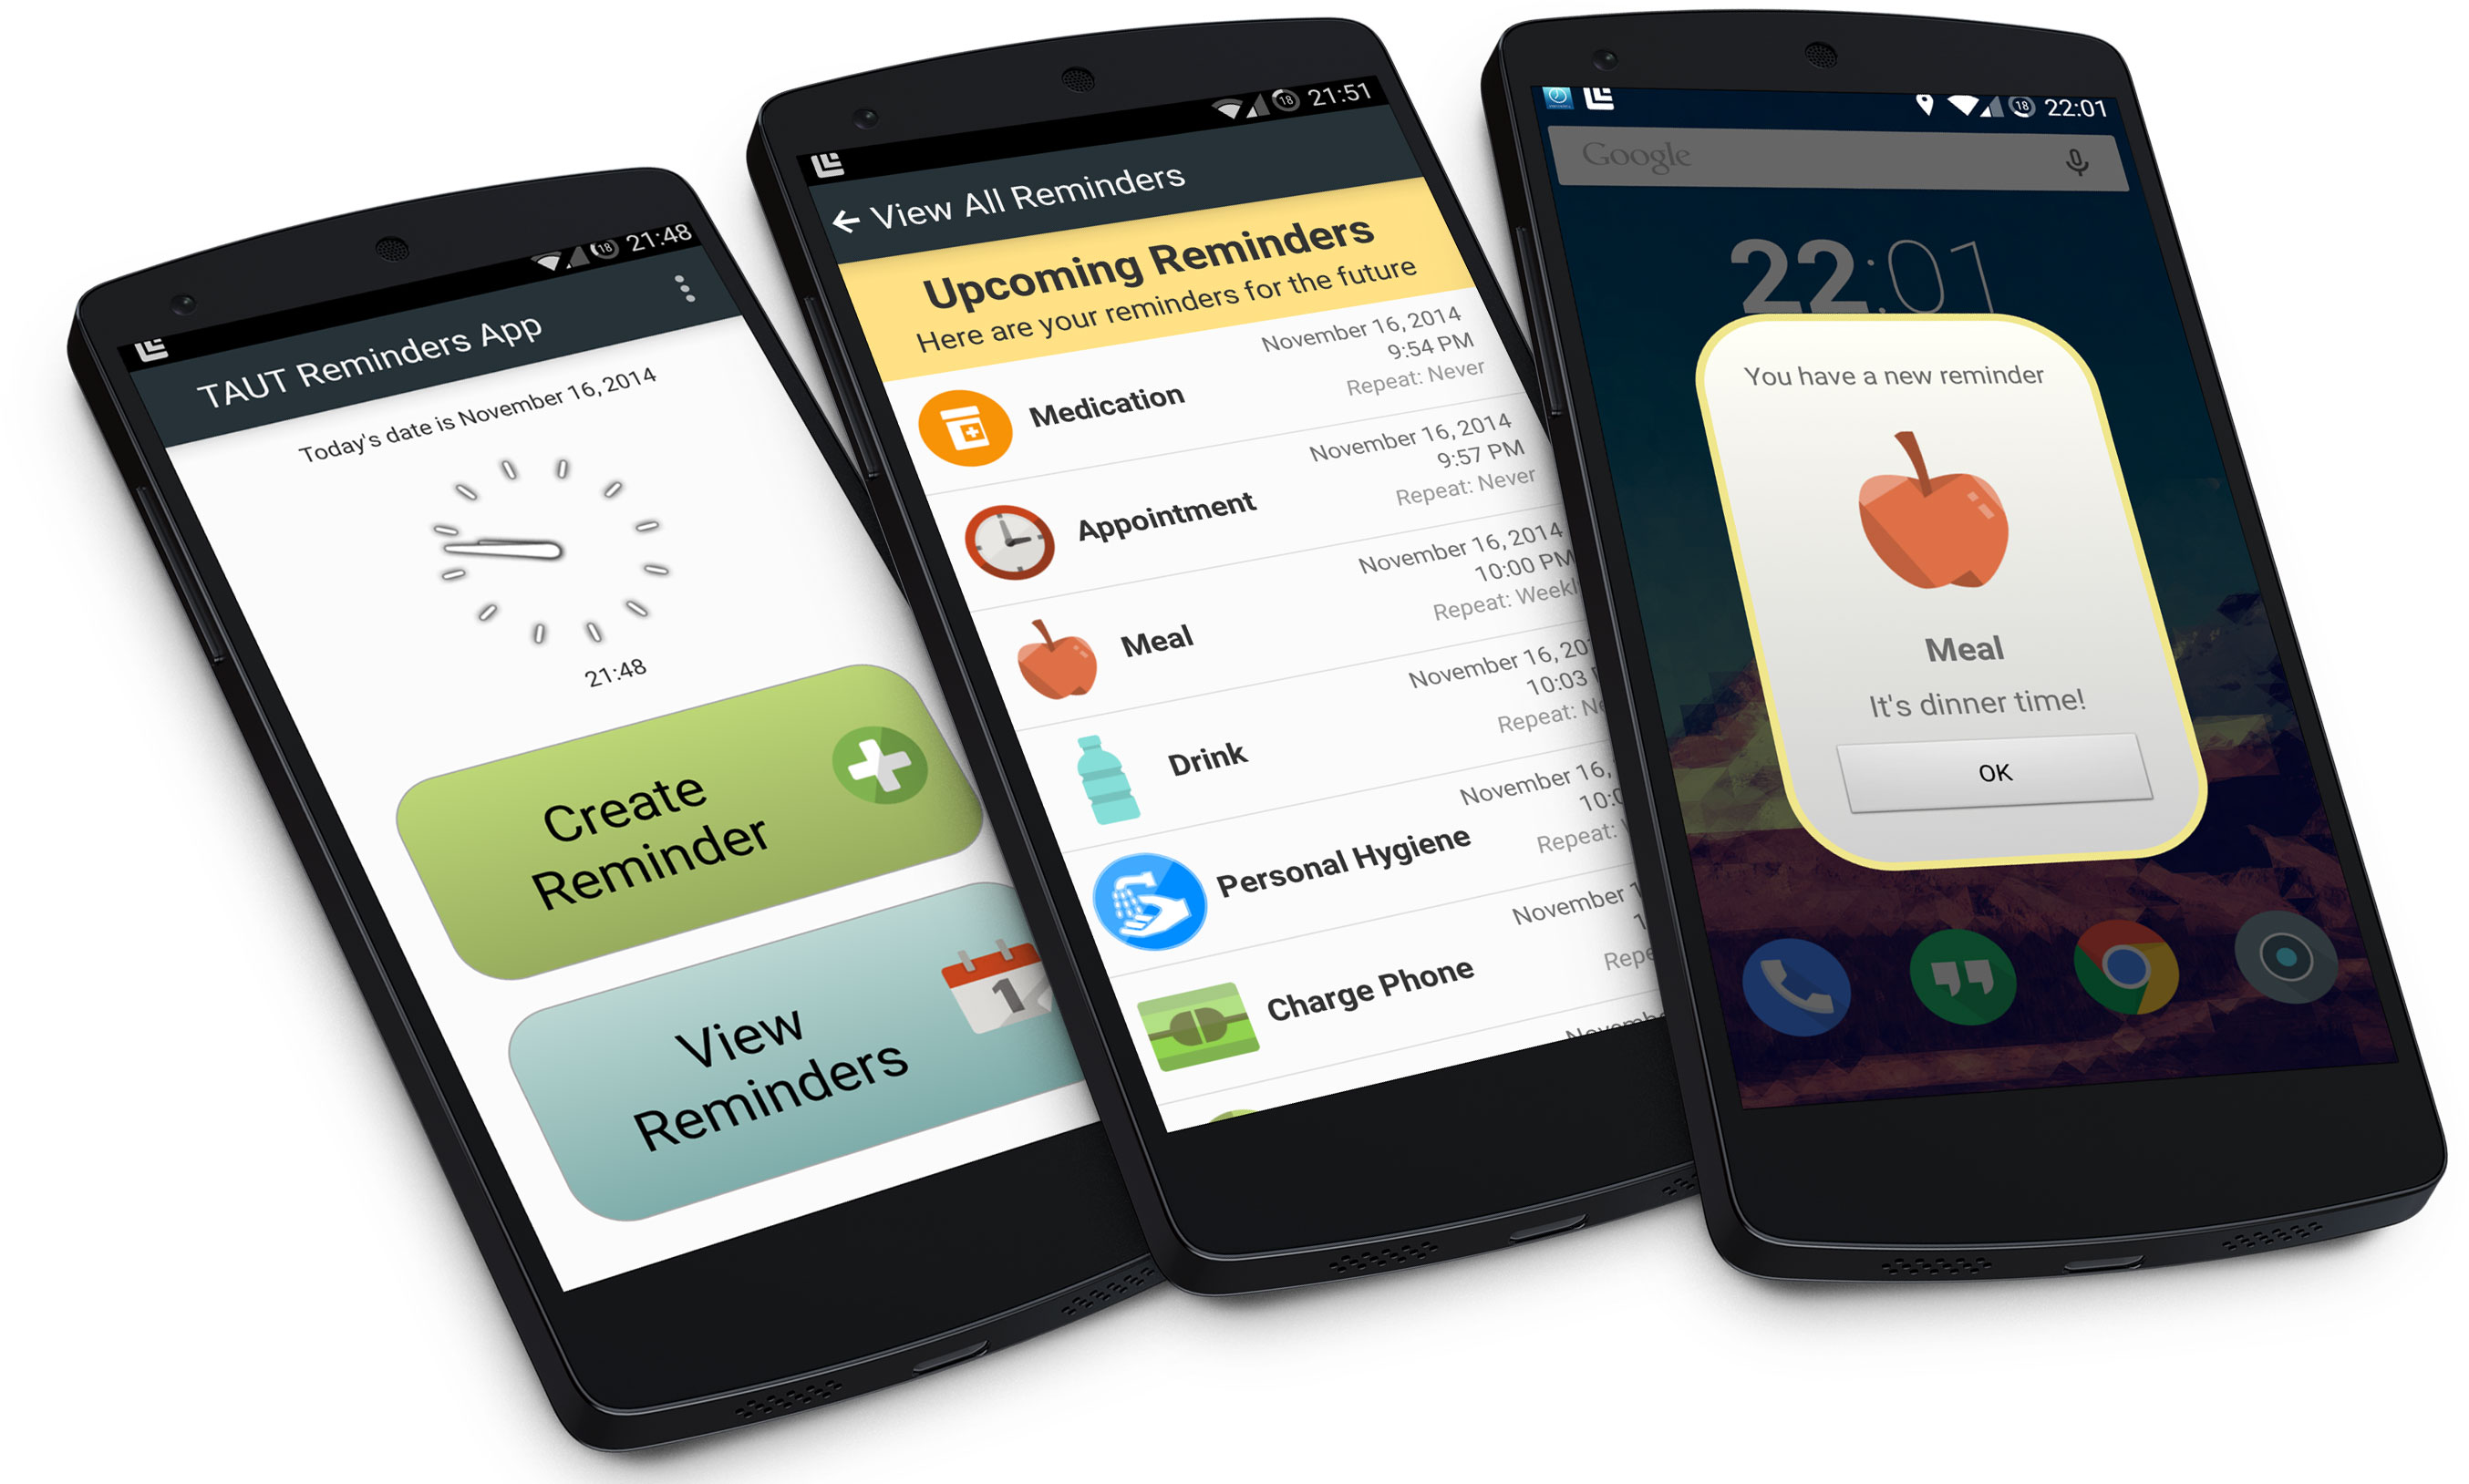
\includegraphics[scale=0.13, angle=0]{Files/treatment-study-1/figures/device-app-screenshots}
        \caption{Home screen, Reminder List and Reminder Delivery Popup screens as displayed on Nexus 4 devices.}
        \label{fig: taut-devices}
\end{figure}

\subsubsection{Creating a Reminder}
The reminders can be created and maintained by the PwD, or by a proxy, such as a caregiver or family member. Using the wizard style approach, the user is guided through the procedure, confirming their choices at each step, as shown in Figure \ref{taut-remindercreation}. Each reminder can be attributed to one of seven ADL types (Meal, Drink, Medication, Hygiene, Appointment, Other, Charge Phone).
The reminders are temporal based, and so the user is asked to confirm the date and time they wish to receive the reminder (Figure \ref{fig: remindercreate-time}), which can also be configured to repeat on a daily, weekly, monthly or custom pattern (Figure \ref{fig: remindercreate-repeat}). At the end of the process, the user is asked to confirm their choices, as per the usability guidelines mentioned earlier.
To provide additional functionality, the ability to record audio messages has also been included. In a similar study, it was noted that coupling voice-based audio recordings with textual descriptions were more effective than video based reminders for PwD \cite{ONeill2010}.

\begin{figure}[h]
    \centering
    \begin{subfigure}[t]{0.3\textwidth}
        \centering
        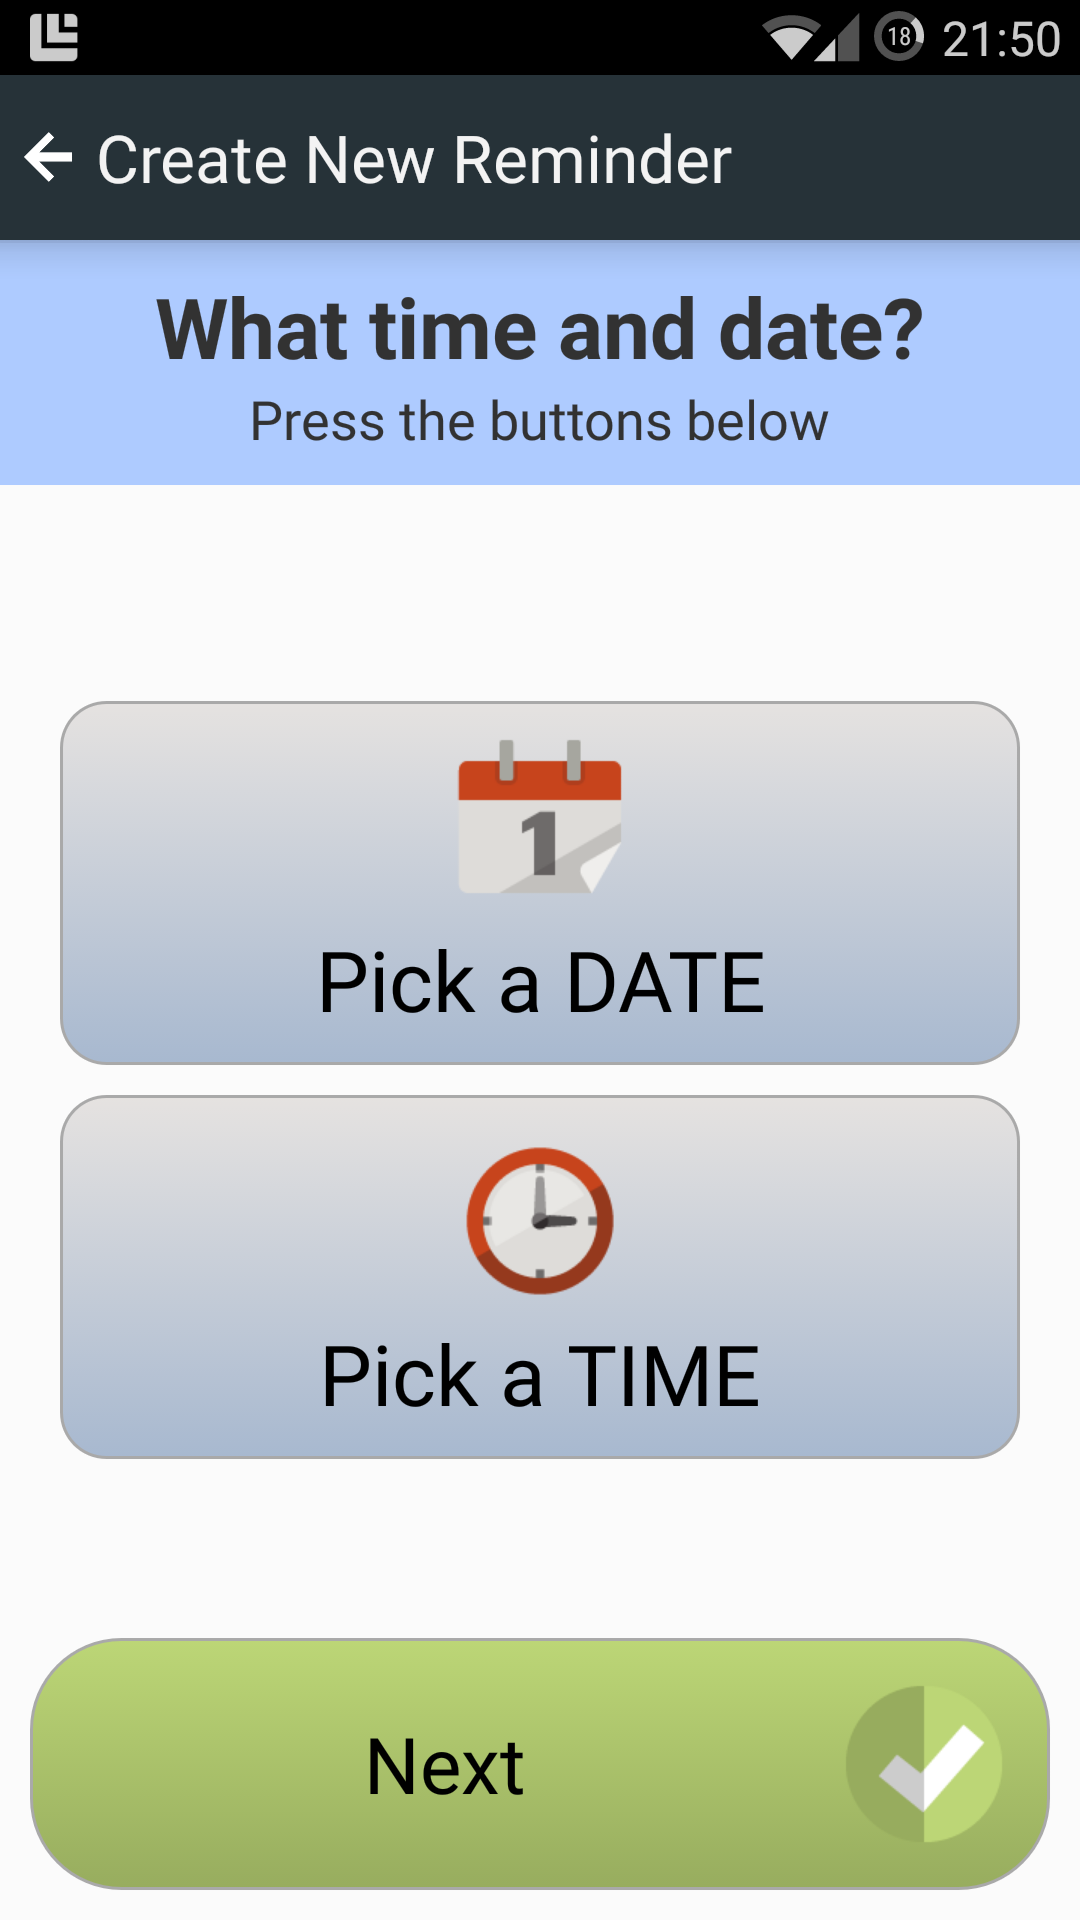
\includegraphics[width=\textwidth]{Files/treatment-study-1/figures/app-remindercreate-1}
        \caption{Date and Time selection screen}
        \label{fig: remindercreate-time}
    \end{subfigure}
    \hfill
    \begin{subfigure}[t]{0.3\textwidth}
        \centering
        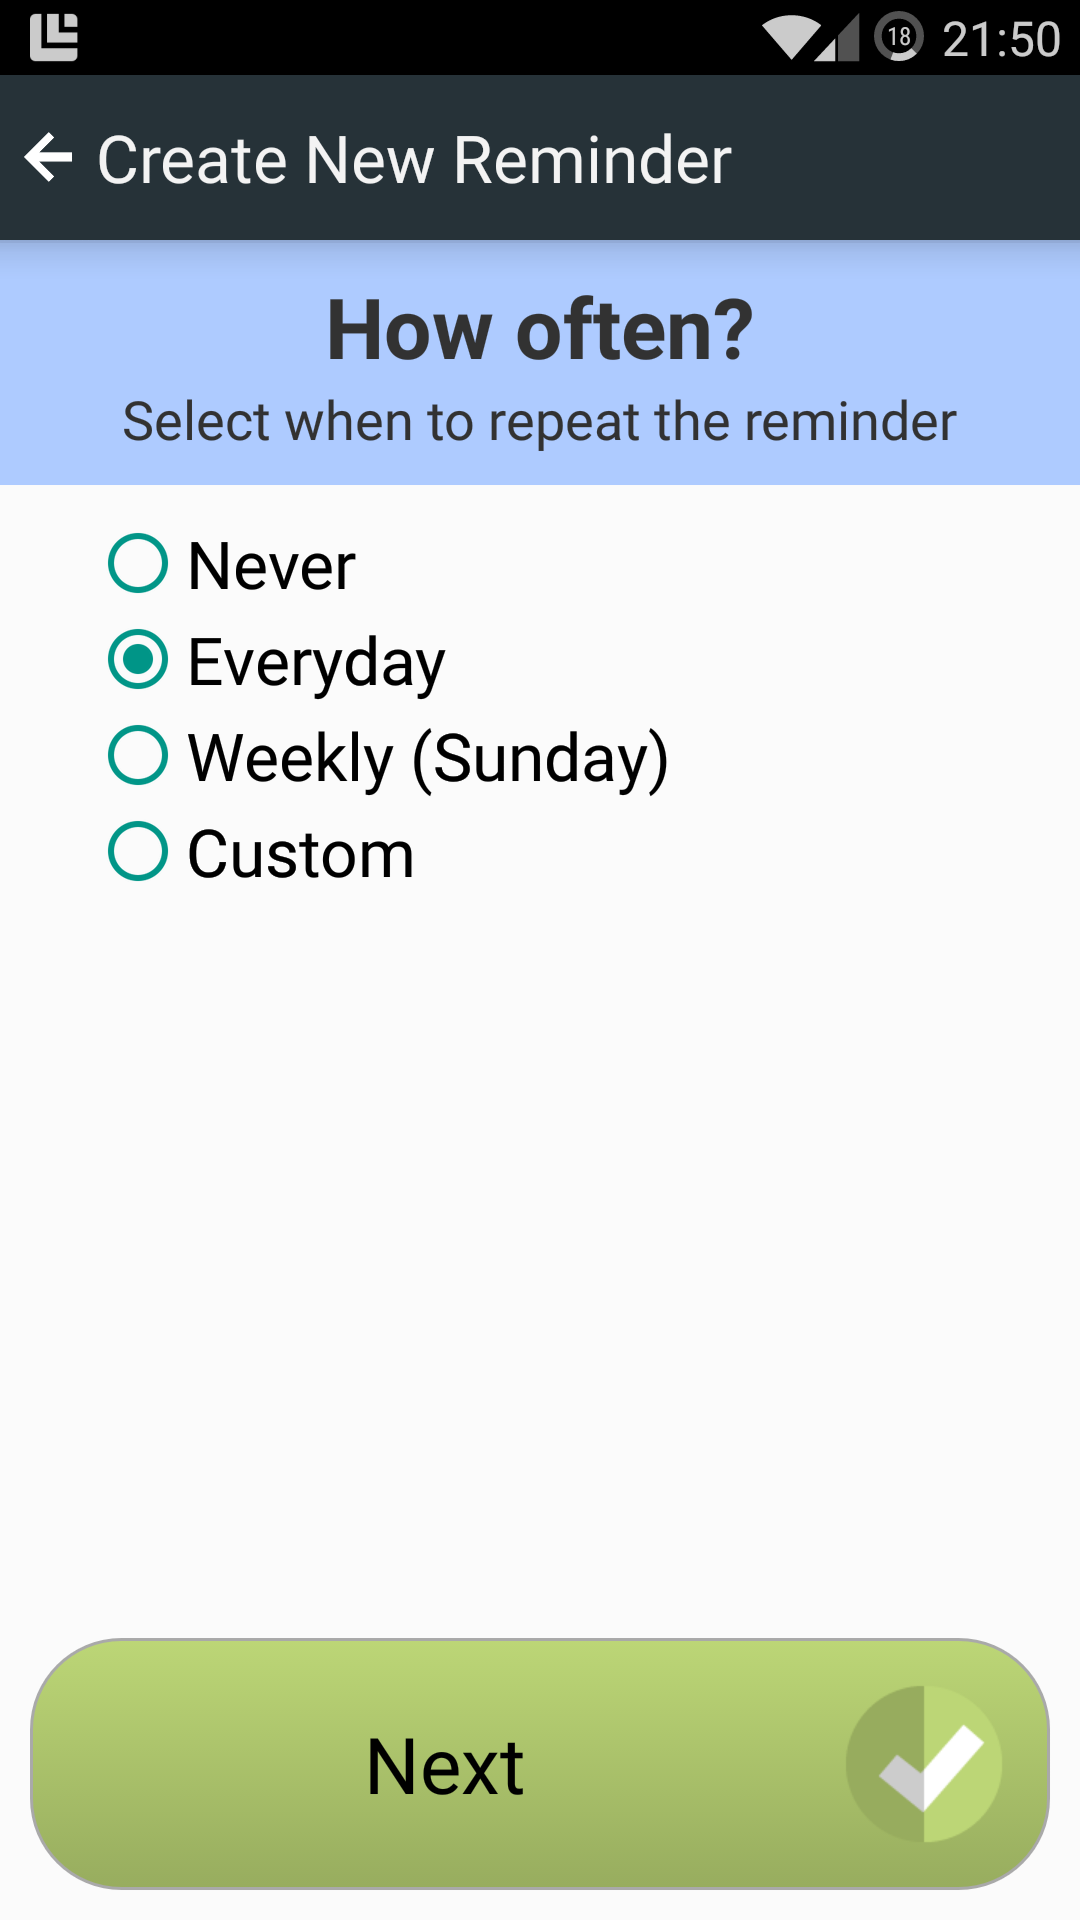
\includegraphics[width=\textwidth]{Files/treatment-study-1/figures/app-remindercreate-type}
        \caption{Repeat Selection}
        \label{fig: remindercreate-repeat}
    \end{subfigure}
    \hfill
	\begin{subfigure}[t]{0.3\textwidth}
        \centering
        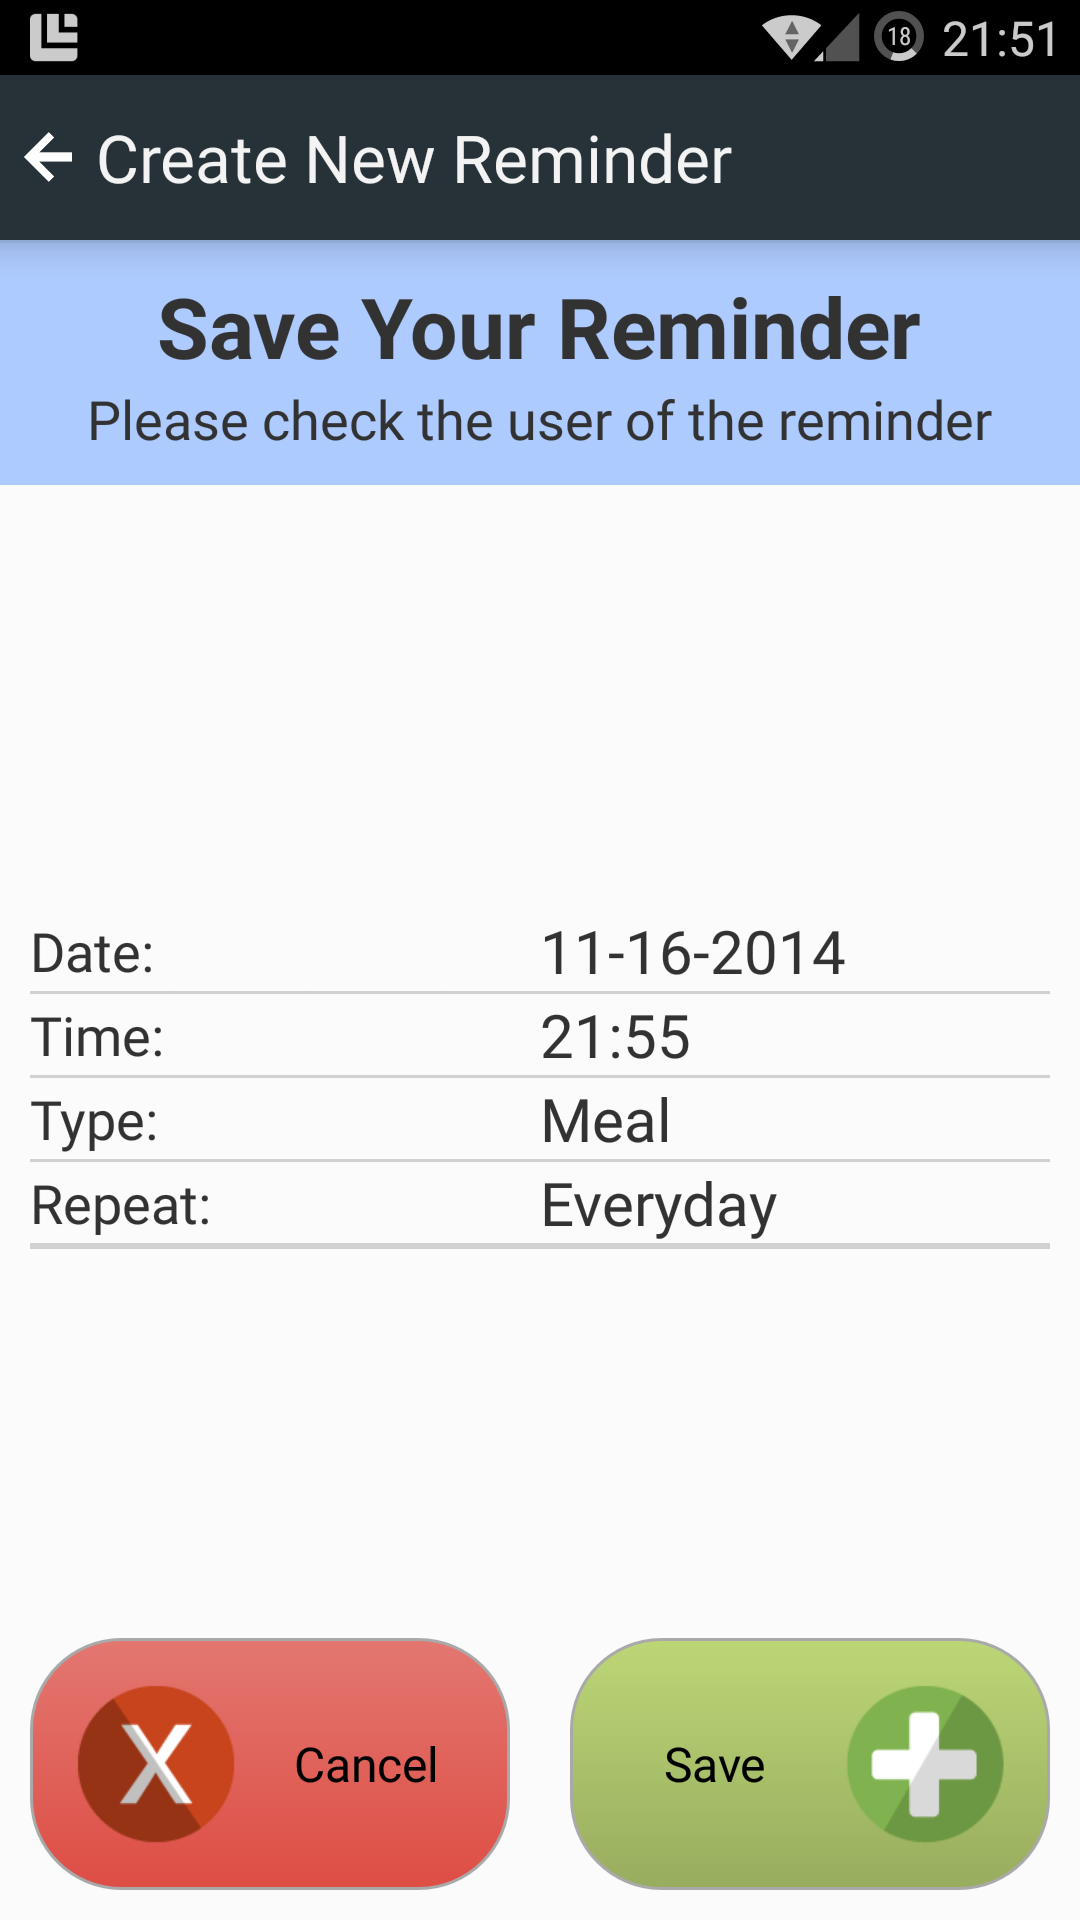
\includegraphics[width=\textwidth]{Files/treatment-study-1/figures/app-remindercreate-confirmation}
        \caption{Confirmation of selected settings}
        \label{fig: remindercreate-confirmation}
    \end{subfigure}
    \caption{Step-by-step reminder creation making use of consistent UI elements, bold text and pastel colours.}
    \label{fig: taut-remindercreation}
\end{figure}

When each reminder was created, a Reminder object (Listing \ref{code: reminderobject}) was stored on the devices local SQLite database, and displayed to the user in the View Reminders screen (Figure \ref{fig: taut-reminderslist}).

\begin{listing}[ht]
\inputminted[
frame=lines,
framesep=2mm,
baselinestretch=1.2,
linenos
]{java}{Files/treatment-study-1/code/Reminder.java}
\caption{Java implementation of a Reminder object.}
\label{code: reminderobject}
\end{listing}
%VIVA: it is probably too late now,  however,  a software architecture or class diagram would maybe have been useful.  Perhaps yu could prepae this after you submit.
\subsubsection{Reminder Delivery} \label{subsubsection: android-alarmmanager}
The delivery mechanism of the reminders makes extensive use of Android's AlarmManager class \cite{GoogleAndroid2016}, enabling each reminder to become a system service. Upon the introduction of Android API 19 (Kit Kat), alarm delivery is inexact, as the operating system will shift alarms in order to minimise wake-ups and battery use. To counter this, the app was explicitly designed to disable the CPU's wake locks as long as the alarm receiver was executing. This guaranteed that the phone would not sleep, or allow another process to interrupt, until each reminder has been delivered, at the cost of battery life.
Each reminder, when delivered, was displayed as a popup dialog box as shown in Figure \ref{fig: taut-reminderpopup}. The popup contained an icon indicating the type of ADL and a textual description of the action the user should perform. As per the recommendations by \citeauthor{CenterforPersonswithDisabilities2015} \cite{CenterforPersonswithDisabilities2015}, a melodic audible tone also accompanied the reminder’s visual delivery.

\subsubsection{Reminder Acknowledgment}
Upon delivery, the user has a time window of 60 seconds in which to acknowledge the reminder. After which, the popup dialog closes, the tone stops playing, and the reminder is logged as ‘missed’. If acknowledged within the 60 seconds the reminder is logged as ‘acknowledged’ and the popup closes. The time taken to acknowledge each reminder instance is also logged.
For voice-based messages, delivery is altered slightly: The user has 60 seconds in which to acknowledge the reminder by playing the voice message. They can re-listen to this voice message as many times as they wish to ensure clarity.
Upon the delivery of each reminder, an acknowledgement object is created, containing a copy of the original reminder object (Listing \ref{code: acknowledgementobject}). In addition to the acknowledgement status of the reminder the object contains the uniqueId of the user, the time taken to acknowledge (if acknowledged), the battery level percentage at the point of delivery, and if an audio reminder the number of times the message was listened to.

\begin{figure}[]
    \centering
    \begin{subfigure}[t]{0.48\textwidth}
        \centering
       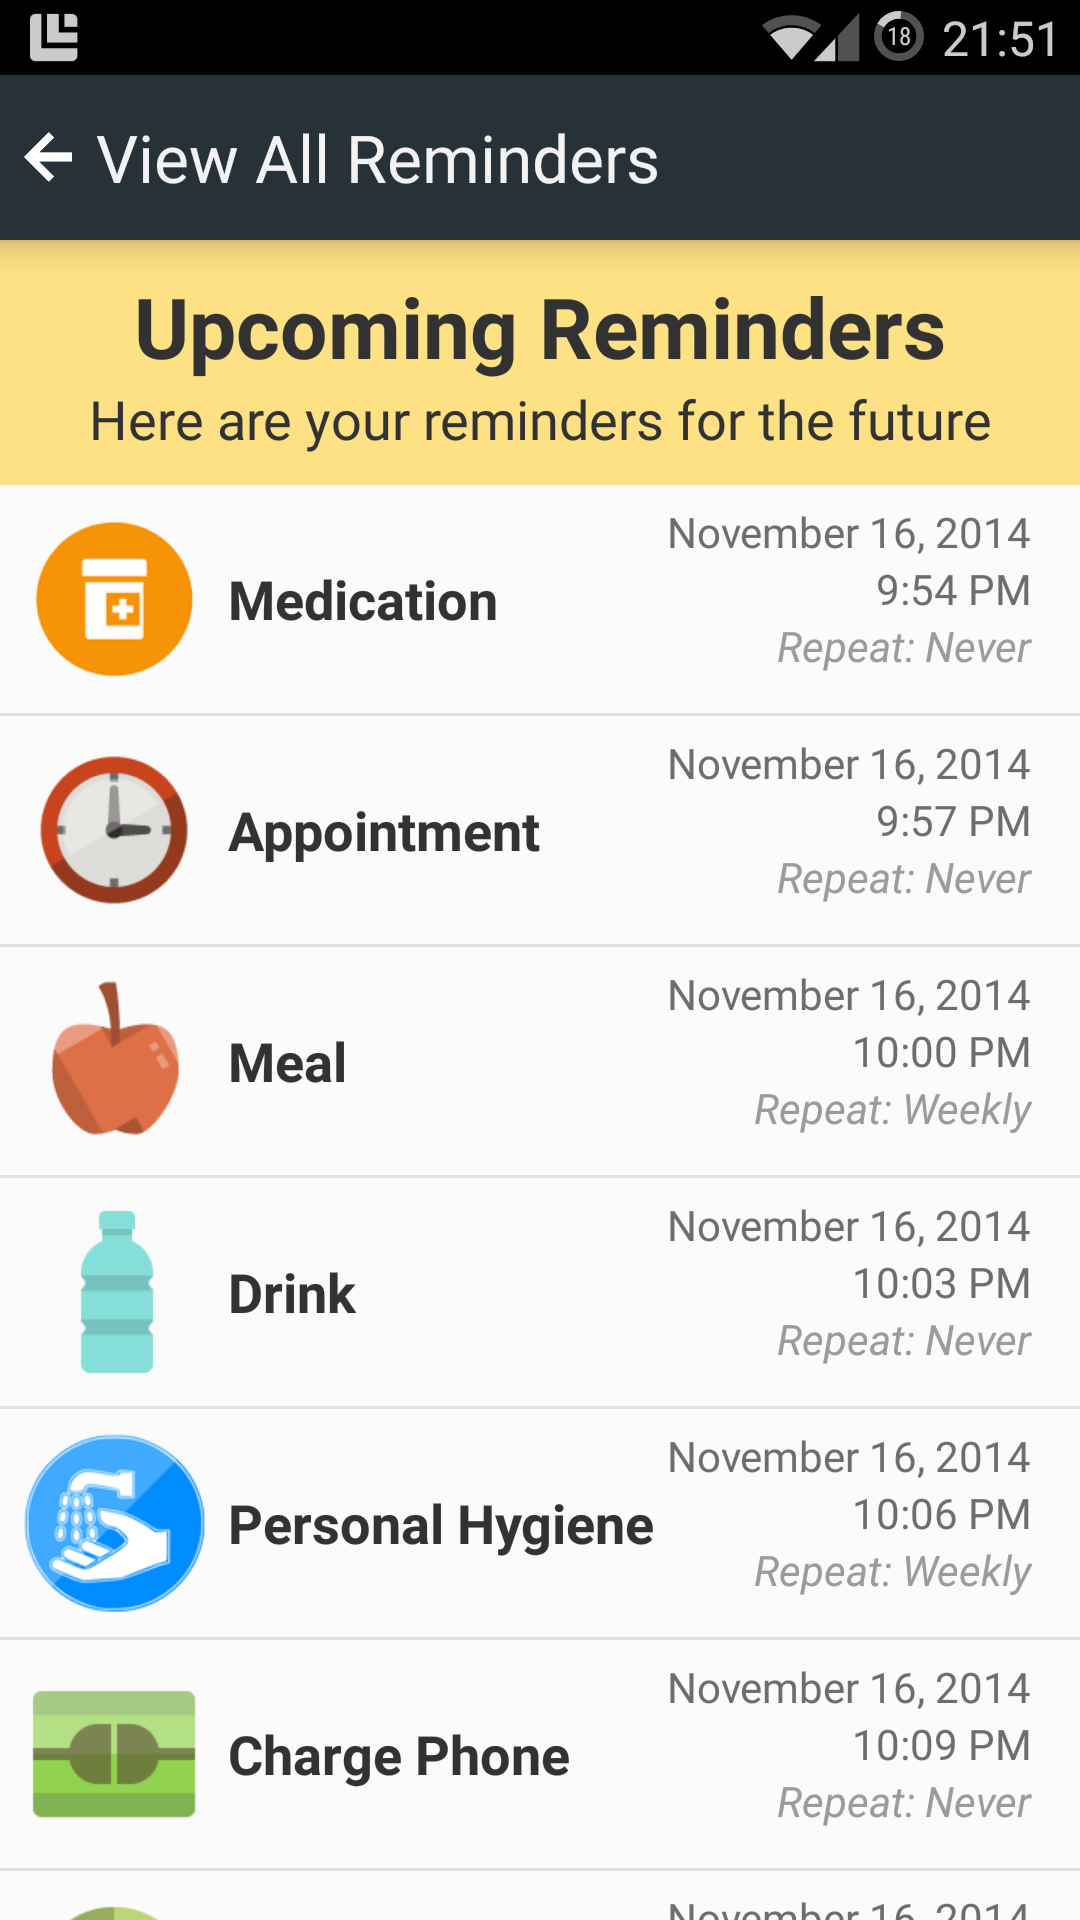
\includegraphics[width=\textwidth]{Files/treatment-study-1/figures/app-reminderslist}
        \caption{View reminders screen displaying all reminders scheduled to be delivered in the future.}
        \label{fig: taut-reminderslist}
    \end{subfigure}
    \hfill
     \begin{subfigure}[t]{0.48\textwidth}
        \centering
      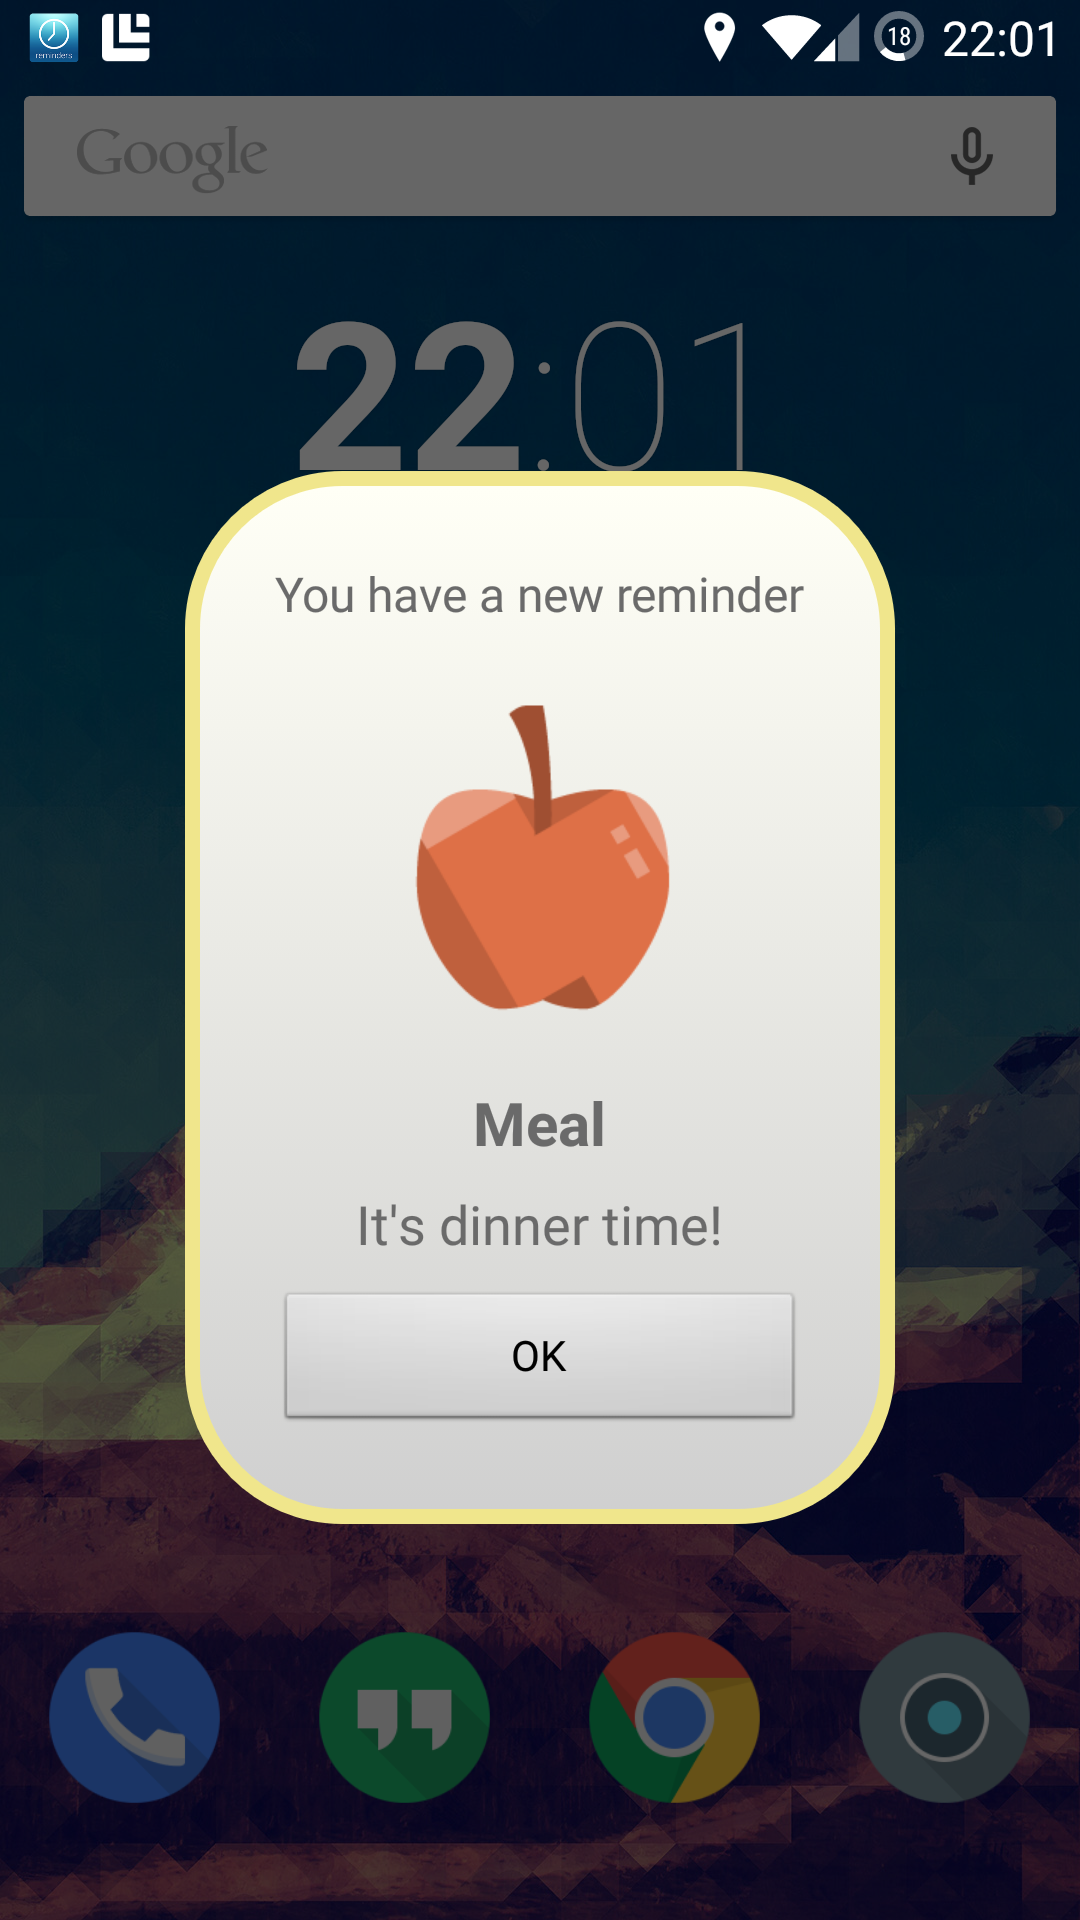
\includegraphics[width=\textwidth]{Files/treatment-study-1/figures/app-reminderpopup}
        \caption{Reminder delivery as a dialog popup with accompanying sounds.}
        \label{fig: taut-reminderpopup}
    \end{subfigure}
      \caption{Reminders scheduled and delivery popups.}
    \label{fig: taut-reminderlist-delivery}
\end{figure}

\begin{listing}[ht]
\inputminted[
frame=lines,
framesep=2mm,
baselinestretch=1.2,
linenos
]{java}{Files/treatment-study-1/code/Acknowledgement.java}
\caption{Java implementation of an Acknowledgement object. The acknowledgement object also contains an immutable copy of the original Reminder object that created it.}
\label{code: acknowledgementobject}
\end{listing}

\subsection{Usage Data Collection Tool}
To support the collection of insightful usage data for the TAUT project, the app records various metrics based upon a user’s interactions with the app. These metrics can be categorised as usage behaviours and reminder data.
\newline \textbf{Usage behaviour} relates to a user’s active engagement with the app, such as how the user navigates the screens of the interface, how long they spend on each screen and how often they launch the app.
\newline \textbf{Reminder data} contains all the relevant information on previously delivered and future scheduled reminders. From high-level analysis of reminder data it is possible, for each individual, to establish the most common ADL type that requires assistance, establish their preferences for voice or text-based reminders and also view who typically creates the reminders.
From this data, it is also possible to perform analysis on the time taken to acknowledge a reminder as shown previously in Listing \ref{code: acknowledgementobject}. From this metric, it is possible to calculate a baseline or average response time and observe for sudden or atypical increases. It is hypothesised that a change in this value, indicating slower reaction times, has the potential to be used as an indicator of further cognitive decline, or disengagement from the technology \cite{Phillips2013}.

\subsubsection{Reminder Acknowledgement}
Regarding adoption, and efficacy of the reminder device, the most pertinent of the data recorded is within the delivered reminders. Analysis of the delivered reminders exposes the number of reminders missed or acknowledged, from which a single metric of an individual’s adherence to the system can be established. To avoid the inclusion of false negatives, the app can detect if a reminder has been missed due to the device being in a powered off state, rather than a lack of human interaction. These instances are logged as a separate value.
The use of this acknowledgement status plays a key role in labelling contextual data observed from the sensors.

\subsection{Contextual Observation}
In the study a key focus is to observe how the PwD interacts with the device, whilst the author hypothesises that contextual observations may be used to make these interactions more consequential and effective. A key component of this approach is to observe the contexts at the time of interaction with the device, and specifically around the point in time when reminders are acknowledged or missed.
\subsubsection{Observation Window}
The time period in which the reminders are scheduled for delivery presents a suitable window in which to observe controlled and understood contextual information. By observing the contexts in this window it may be possible to associate certain sensor states with acknowledged or missed reminders.
For the purposes of this study the app has been configured to record the raw outputs of all available sensors 3 minutes prior to a reminder being delivered, and continues to record data for 3 minutes after the reminder has been delivered. This creates a number of sensor output files, with a total recording duration of 6 minutes, for each available sensor.
Unix timestamps (ms) are used to enable synchronicity across the various recordings.
During initial beta testing of the app, it was shown that a 6 minute window provided a good balance of contextual information, whilst keeping file size relatively low \cite{Hartin2014-EMBC}. A typical set of 6-minute recordings from the Moto G, using all available sensors, records at approximately 130KB/min.

\subsection{Sensor Platforms}
As the app has been developed for android smartphones, it is possible to utilise a variety of on-board sensors to observe and record contextual information. The android platform groups their array of available sensors into 3 main categories: motion, positional and environmental.

\subsubsection{Motion}
Within the android platform there are 2 core hardware based motion sensors, the accelerometer, and the gyroscope. The sensors capture acceleration and rotation forces along 3 dimensions, or axes. These sensors measure acceleration forces and rotational forces along three axes. The category also includes gravity sensors and rotational vector sensors.
In the android platform, where a hardware sensor is missing, in many cases a simulated sensor can be generated from the input of another, e.g. using the accelerometer and magnetometer to simulate a gyroscope.
Previous studies have relied heavily upon the use of accelerometers for the classification of physical activities, and gyroscopes are often use in conjunction, strengthening the classifiers \cite{Wu2012, Preece2009}. In many cases, these sensors require additional processing to extract relevant information. For example, the accelerometer, measures the acceleration applied to the device, which\textit{includes the force of gravity}. Many previous studies using standalone accelerometers must calibrate and apply a high-pass filter to isolate the true rate of acceleration \cite{Ferraris1995}. The android platform makes it possible to record this true acceleration (minus gravity) directly from the device, with the caveat that it always has an offset, which needs to be removed through calibration.

\subsubsection{Positional}
Positional sensors provide information that can determine the position of the device. These consist of the magnetometer, the orientation sensor and the proximity sensor.
The magnetometer provides information regarding orientation across 3-axes. The orientation sensor is an emulated sensor using calibrated data from the raw magnetometer data, and provides provides the azimuth (yaw), pitch, and roll values.
Magnetometers have been used in combination with accelerometry data for the classification of human activities in similar studies \cite{Zhang2015,Catal2015}.
The proximity sensor provides a measure of distance between the sensor and an object. The sensor is forward facing, and is primarily used by the operating system to turn the screen off if the sensor is occluded, signifying that the user has the phone close to their face, or in their pocket, to avoid accidental presses. In this study, however, the proximity sensor is expected to provide refining information in a number of scenarios. E.g. movement is observed in the accelerometer, and the proximity sensor shows the phone is not occluded. This may indicate that the phone is in the user's hand, resulting in an opportune time to deliver a reminder \cite{Hoseini-Tabatabaei2013}. Unlike the accelerometer and magnetometer, who return multidimensional arrays of data, the proximity sensor returns a single value when polled.

\subsubsection{Environmental}
Environmental sensors aim to observe various environmental properties, including illumination, air temperature, air pressure, and humidity. To perform these readings, the smartphone requires a photometer, thermometer and barometer, all of which are hardware based. As such, the inclusion of these sensors is scarce, with the light sensor (photometer), being the most commonly included by device manufacturers. As with the proximity sensor, the light sensor returns a single illuminance (lux) reading when polled. These sensors require no calibration. The values from these sensors are not expected to yield sufficient data for an accurate context aware system, however, their fusion with the other sensor types may refine and influence a classifier.


\subsection{Device Consistency} \label{subsection: taut-deviceconsistency}
A downside to developing for the android platform, is that the selection of sensor modalities is at the manufacturers discretion. This means that the number of sensor platforms which are available vary across devices. Given that this is a scientific study, steps were taken to ensure consistency across the cohort. Taking into consideration the cost to sensor ratio, it was decided that the Motorola Moto G smartphone was an appropriate choice for the study. The Moto G is equipped with an accelerometer, magnetic field sensor, proximity sensor, light sensor and a GPS receiver chip. Ulster University's Ethical Committee approved the use of all sensors, with the exception of the GPS, due to privacy concerns. As such, the remaining 4 sensors were used, which still address the 3 main sensor categories of the android platform, and are consistent with the sensors used in similar studies \cite{Poppinga2014}.

\subsection{Internet Connectivity}
Initial analysis of the intended study cohort's location uncovered sparse internet connectivity, both in the home and via mobile networks. This influenced the design of the data model, resulting in an offline-first app, storing all recorded data, both usage (SQLite) and sensor (CSV), on the local disk, negatively impacting data redundancy. To mitigate the risk of losing data, the app was also programmed to be opportunistic with connectivity. If an internet enabled connection was detected (3G, LTE, or Wi-Fi), the app would attempt to send the reminder acknowledgement data to a remote MySQL server with a low overhead in JSON format. The raw sensor data would be to large to send via an opportunistic connection, and so physical access to the handset would still be required to retrieve the data.

\section{Testing and Evaluation}
To ensure that the developed application and context-aware sensor framework was fit for purpose, the app was deployed to an internal testing and evaluation cohort at Ulster University. Ethical approval to perform the study was granted by Ulster University's Research Ethics Committee (HARTIN001).

\subsection{Objectives}
The testing study had the following objectives:
\begin{itemize}[noitemsep,topsep=0pt]
  \item to investigate the use of the smartphone’s embedded sensors to detect the user’s movement, location and environmental contexts.
  \item to investigate the correlation between the contextual sensor information and observed notification adherence.
  \item to identify the optimal sensor types and combination permutations to provide useful contextual sensor information.
  \item to evaluate the usability of the smartphone platform to provide and gather information from the user.
  \item to create an openly available data set to publish within the research community.
\end{itemize}

\subsection{Recruitment}
Recruitment was performed by email, sent to Engineering and Computing faculty members at Ulster University. 9 healthy members of the Smart Environments Research Group responded and were recruited for the study (Median age: 27). These participants will hereafter be referred to as the test cohort (TC).

\subsection{Study Design}
The study was designed to be a non-randomised controlled study, with a duration of 7 days. Participants were asked to perform a single compulsory task: to set a notification for a time that was convenient to them. If the participants found the notifications useful they may set as many as they wish. In order to investigate variations in context throughout the day, the participants were asked to use the app to assist them with scheduling meals, appointments and other general activities of daily living.

\subsection{Outcome Measures}
The outcome measures of the study included quantifying the number of reminders set by each participant, calculation of their acknowledgement rate and the types of reminders set. In addition offline analysis, labelling, and initial classifier modelling was performed on the sensor data to ensure the data was fit for purpose. Details of data modelling and classification results are detailed in Section \ref{section: taut-results}.

\subsection{Results}
Having collected the data from the TC, adoption, usage and sensor data were analysed.

\subsubsection{Adoption and Usage}
As a data collection tool the app performed its intended role. An overview of the reminder statistics are presented in Table \ref{tbl: taut-pilot-reminders}. In total 223 reminders were scheduled to be delivered during the evaluation period, of which a total of 73\% (163) were acknowledged with a mean response time of 12.38 seconds. Upon further analysis it was discovered that 23.33\% (14) of the missed reminders were due to the device being in a powered off state. Many of reminders were set to repeat daily at the same time, thus potentially increasing their chances to be acknowledged \cite{Hartin2014-EMBC}.
%VIVA: Question - Why does this increase the chances to be acknowledged?

\begin{table}[h]
\centering
\caption{Reminder acknowledgement statistics for internal testing and evaluation study}
\label{tbl: taut-pilot-reminders}
\resizebox{\textwidth}{!}{%
\begin{tabular}{@{}lllllll@{}}
\toprule
Participant & \begin{tabular}[c]{@{}l@{}}Reminders \\ Set\end{tabular} & \begin{tabular}[c]{@{}l@{}}Acknowledged\\ (count)\end{tabular} & \begin{tabular}[c]{@{}l@{}}Acknowledged\\ (\%)\end{tabular} & \begin{tabular}[c]{@{}l@{}}Missed\\ (count)\end{tabular} & \begin{tabular}[c]{@{}l@{}}Missed\\ (\%)\end{tabular} & \begin{tabular}[c]{@{}l@{}}Mean \\ response\\ time (s)\end{tabular} \\ \midrule
P01 & 47 & 32 & 68.09\% & 15 & 31.91\% & 14.26 \\
P02 & 9 & 6 & 66.67\% & 3 & 33.33\% & 16.32 \\
P03 & 8 & 8 & 100.00\% & 0 & 0.00\% & 11.89 \\
P04 & 20 & 15 & 75.00\% & 5 & 25.00\% & 11.56 \\
P05 & 7 & 6 & 85.71\% & 1 & 14.29\% & 5.6 \\
P06 & 39 & 35 & 89.74\% & 4 & 10.26\% & 12.96 \\
P07 & 34 & 25 & 73.53\% & 9 & 26.47\% & 9.03 \\
P08 & 17 & 12 & 70.59\% & 5 & 29.41\% & 14.61 \\
P09 & 42 & 24 & 57.14\% & 18 & 42.86\% & 15.17 \\ \midrule
Total & 223 & 163 & 686.47\% & 60 & 213.53\% & 96.23 \\
Mean & 24.7 & 18.1 & 73.09\% & 6.6 & 26.91\% & 12.38 \\ \bottomrule
\end{tabular}
}
\end{table}

\subsubsection{Sensor Recording}
The app also fulfilled its function as a context-gathering tool, recording 6-minute windows of sensor data for each of the reminders delivered. Each time-series based recording (accelerometer and magnetometer) required 2.6 MB of hard disk space. When compressed, the size was reduced to 430kb.
Rudamentary analysis of the acknowledged reminders observed in the TC cohort shared a similar pattern. The pattern which was observed was if the device was static, showing minimal movement in the accelerometer signal, and also reading low light levels, the reminders were predominately acknowledged.
 A post-evaluation questionnaire, performed by a subset of the TC (n=5), revealed that this may be due in part to the similarity of the activities they performed during the study, such as working at a desk or attending meetings, performed daily by 100\% and 80\% of the respondents respectively \cite{Hartin2014-EMBC}.
Placement of the smartphone was also similar across the respondents, with their smartphones placed on their desks (100\%), or in their trouser pockets (left pocket: 40\% and right pocket: 60\%) for the majority of the use cases. The questionnaire also revealed that the top 4 reasons for missed reminders within the cohort were:

\begin{enumerate}[noitemsep,topsep=0pt]
	\item Otherwise engaged in an activity (100\%)
	\item Not carrying smartphone (80\%)
	\item Did not hear the notification (60\%)
	\item Reminder was not loud enough (40\%).
\end{enumerate}

\subsection{Observations and Improvements} \label{subsection: improvements}
As highlighted in Section \ref{subsection: taut-deviceconsistency}, the trial study cohort's intended device was the Motorola Moto G, from which all development and pre-release testing was based. Upon deploying the app to each participant's personal smartphone for the evaluation a number of observations were made.
Firstly, those with older devices noticed increased battery drain and slower average response times for other apps, when future reminders were scheduled. Replicating these conditions after the study uncovered the cause to be the implementation of the reminder delivery mechanism. As noted earlier in Section \ref{subsubsection: android-alarmmanager}, the android platform's delivery of time based notifications is accurate, however, not to a degree of milliseconds. In an effort to ensure perfect synchronicity between the reminder delivery, and the midpoint of the sensor recording, the author used a thread that continuously checked the current unixtime against that of the upcoming reminder. Whilst acceptable in theory, the inefficiency of this approach was noted on less powerful devices, and was subsequently removed before deployment to the main demented study cohort. To ensure synchronicity between sensor recordings and the reminder delivery in later versions, the exact unixtime to a millisecond precision is recorded as part of the reminder object, and synchronisation is performed retrospectively.
The second observation was made during the analysis of sensor data. As stated earlier, it is to the discretion of the handset manufacturer which hardware they include in their devices. Amongst the TC, there was an observable difference in the calibration offset and sampling rates of the accelerometer data. The reasons for this, and methods to rectify are presented later in the Chapter, with particular focus in the pre-processing section.

\section{Study with PwD}
Having improved the performance and stability of the app based upon the findings during testing, the app was then deployed to the intended study cohort, 30 PwD based in Cache County, Utah.

\subsection{Study Design}
The app was designed as the principle technology component for the TAUT project, a collaborative project between Utah State University (USA), the University of Utah (USA) and Ulster University (UK).
The project integrates data from two large databases, the Cache County Study on Memory in Aging (CCSMA) and the Utah Population Database (UPDB) in an effort to build a user profile. The CCSMA is a longitudinal, population based study of AD and other dementias, which has followed over 5,000 elderly residents of the Cache County, Utah (USA) for over twelve years (1995-2007) \cite{Tschanz2013}. The UPDB contains genealogical, medical, vital and demographic records, with full coverage of medical information spanning the past 20 years for over 7 million people.

\subsubsection{Recruitment}
From the integrated dataset, a subset of 125 individuals showing the greatest decline in cognition, evaluated by a 3MS \cite{Tschanz2002}, were identified as being suitable for the study. From this 125, 30 were screened and recruited for the study (Figure \ref{fig: taut-recruitment}). These participants are hereafter referred to as the Dementia Cohort (DC).

\begin{figure}[h]
    \centering
        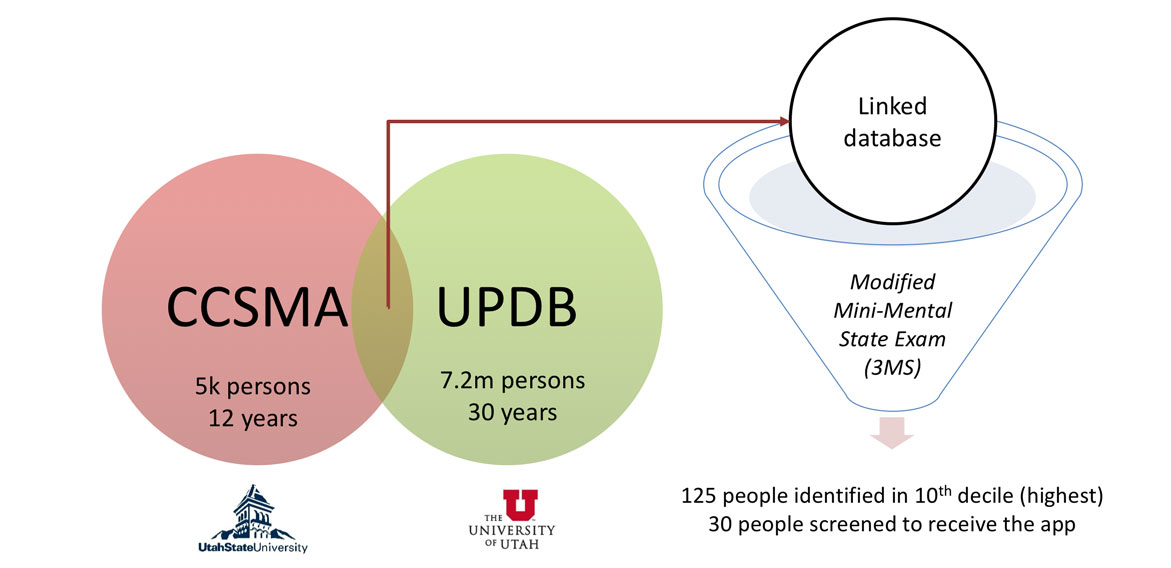
\includegraphics[scale=0.3, angle=0]{Files/treatment-study-1/figures/taut-recruitment}
        \caption{Recruitment from a subset of participants found in both the UPDB and the CCSMA databases.}
        \label{fig: taut-recruitment}
\end{figure}

\subsection{Deployment to Cohort}
Each smartphone device was preloaded with the TAUT app and physically delivered to each participant by a small team of research associates based at Utah State University, Utah. The study participant, and if possible their carers, were provided with a short training demo as to how the app operated, including instructions how to set, view and acknowledge reminders, and how to charge the device.

\subsection{Post-Study Data Retrieval}
It was understood that the DC would have restricted access to the internet. As stated earlier, in anticipation of this, all data was stored locally on the device, with opportunistic syncing to an online database. A number of visits were scheduled with the cohort to permit the retrieval of sensor data during the study, with the aim of producing snapshots of progress throughout the study, however, many participants were unavailable at their scheduled times. For the sensor data that was retrieved, preliminary and exploratory analysis was performed \cite{Hartin2014-WAGER}, however, the datasets were sparse and heavily unbalanced at this point.
At the study close, all the devices, with the exception of 2 which were lost by the study participants, were retrieved, and the raw data was downloaded for processing.

\section{Adoption and Usage by PwD}
This Section will cover the user adoption and usage of the app, with detailed analysis on context-aware results covered later in the Chapter.
Encouraging usage was observed in the initial month, when one of the participant's who had internet access in the home synchronised their data. At this time, the total number of reminders delivered to the user was 215, with a mean acknowledgement rate of 58.1\% \cite{Hartin2014-EMBC}. Upon the study close, however, the total number of reminders set to be delivered to all users was 8881, with a mean acknowledgement rate of 19.2\% (n=1686). It is important to note that the calculation of this metric includes reminders which were missed due to the phone being in a powered off state. Removing these instances resulted in a total of 6289 reminders being truly delivered by the phone, with a mean acknowledgement rate of 26.8\% (\textit{(1686/6289)*100}). This statistic is somewhat skewed by the non-adopters in the study \cite{Cleland2014-IWAAL}. For adopters of the platform, the mean individual acknowledgement rate was 39.2\%. Full statistics for each participant can be found in Table \ref{tbl: taut-reminder-stats} and represented visually in Figure \ref{fig: reminder-stacked-stats}.

\begin{table}[h]
\centering
\caption{Reminder acknowledgement statistics for 30 persons with dementia, ordered by total reminders in descending order.}
\label{tbl: taut-reminder-stats}
\resizebox{\textwidth}{!}{%
\begin{tabular}{@{}lllllll@{}}
\toprule
Participant & \begin{tabular}[c]{@{}l@{}}Number of \\ Reminders\end{tabular} & Acknowledged & Missed & Device Off & Acknowledged \% & Missed \% \\ \midrule
P01 & 2874 & 850 & 1728 & 296 & 33\% & 67\% \\
P02 & 1335 & 379 & 937 & 19 & 29\% & 71\% \\
P03 & 600 & 364 & 172 & 64 & 68\% & 32\% \\
P04 & 557 & 33 & 219 & 305 & 13\% & 87\% \\
P05 & 531 & 6 & 523 & 2 & 1\% & 99\% \\
P06 & 473 & 4 & 207 & 262 & 2\% & 98\% \\
P07 & 472 & 9 & 222 & 241 & 4\% & 96\% \\
P08 & 426 & 1 & 40 & 385 & 2\% & 98\% \\
P09 & 401 & 6 & 9 & 386 & 40\% & 60\% \\
P10 & 229 & 1 & 194 & 34 & 1\% & 99\% \\
P11 & 225 & 2 & 199 & 24 & 1\% & 99\% \\
P12 & 218 & 5 & 22 & 191 & 19\% & 81\% \\
P13 & 94 & 3 & 19 & 72 & 14\% & 86\% \\
P14 & 76 & 3 & 2 & 71 & 60\% & 40\% \\
P15 & 72 & 6 & 66 & 0 & 8\% & 92\% \\
P16 & 71 & 2 & 4 & 65 & 33\% & 67\% \\
P17 & 49 & 1 & 22 & 26 & 4\% & 96\% \\
P18 & 43 & 2 & 18 & 23 & 10\% & 90\% \\
P19 & 28 & 0 & 0 & 28 & - & - \\
P20 & 2 & 2 & 0 & 0 & 100\% & 0\% \\
P21 & 2 & 2 & 0 & 0 & 100\% & 0\% \\
P22 & 2 & 2 & 0 & 0 & 100\% & 0\% \\
P23 & 2 & 1 & 0 & 1 & 100\% & 0\% \\
P24 & 1 & 1 & 0 & 0 & 100\% & 0\% \\
P25 & 1 & 1 & 0 & 0 & 100\% & 0\% \\
P26 & 0 & 0 & 0 & 0 & - & - \\
P27 & 0 & 0 & 0 & 0 & - & - \\
P28 & 0 & 0 & 0 & 0 & - & - \\
P29 & 0 & 0 & 0 & 0 & - & - \\
P30 & 0 & 0 & 0 & 0 & - & - \\ \midrule
Sum & 8784 & 1686.0 & 4603.0 & 2495.0 & 941.8\% & 1458.2\% \\
Mean & 302.8965517 & 58.1 & 158.7 & 86.0 & 39.2\% & 60.8\% \\ \bottomrule
\end{tabular}
}
\end{table}

It may be noted from the Table that there was a large degree of difference between the two main outcomes: acknowledged and missed. The impact of this in the development of the context-aware reminder system is discussed later in the Chapter.

\begin{figure}[h]
    \centering
        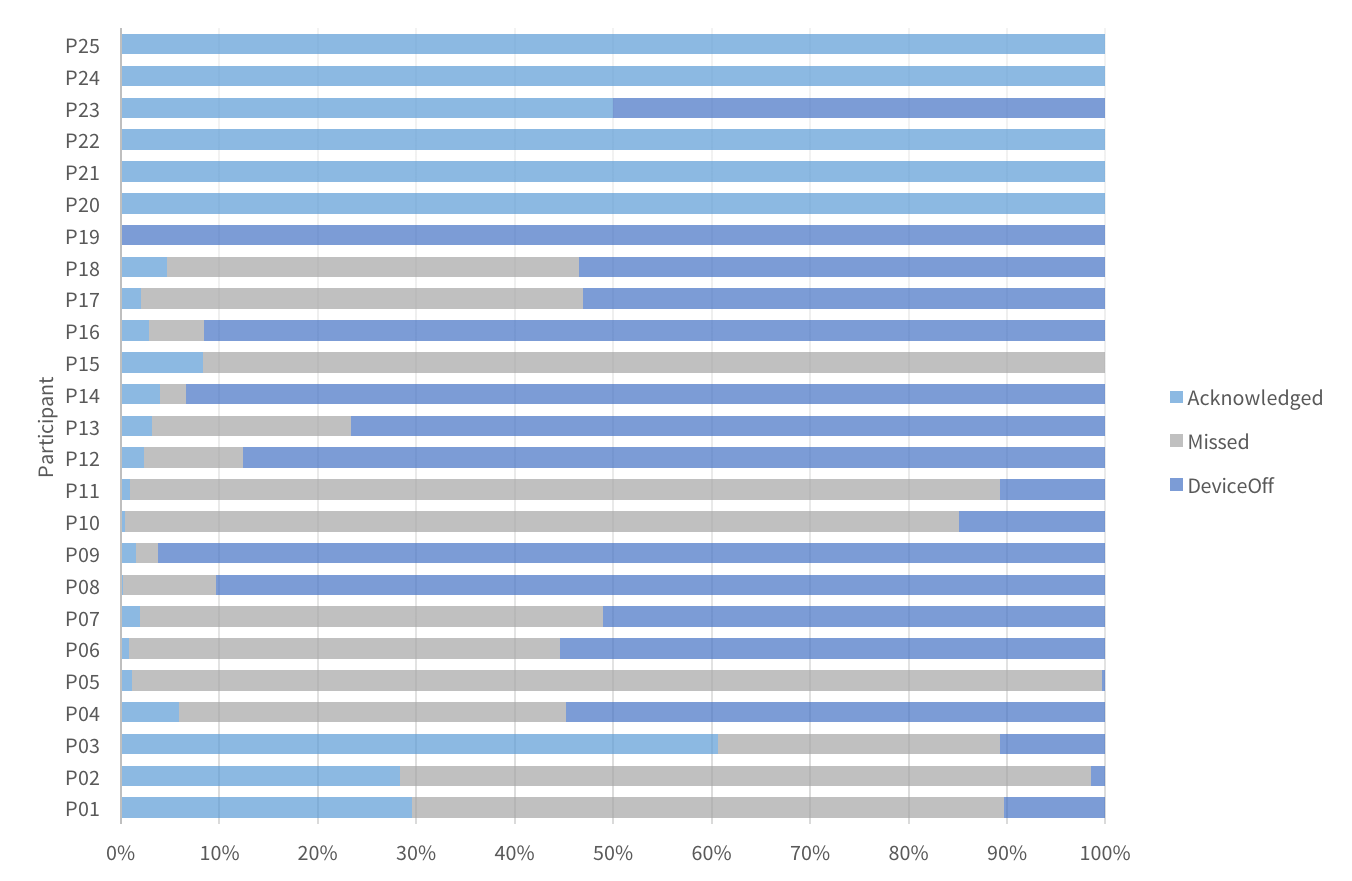
\includegraphics[scale=0.6, angle=0]{Files/treatment-study-1/figures/reminder-stacked-stats}
        \caption{Stacked bar graph showing distribution of scheduled reminders that were Acknowledged, Missed, and Missed due to powered off device.}
        \label{fig: reminder-stacked-stats}
\end{figure}

\subsection{Response Times}
As stated earlier, the time taken to acknowledge a reminder was recorded. It was hypothesised by the author that the change in response time could potentially be correlated with decline of MMSE scores. What was originally observed in the first few months of the study, using the initial data snapshot obtained from the participant who had an internet connection (P03), was that their response times had decreased, as shown in Figure \ref{fig: responsetimedecrease}.

\begin{figure}[h]
    \centering
        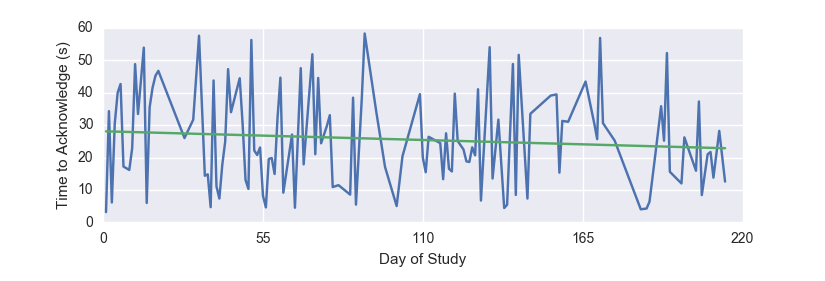
\includegraphics[scale=0.7, angle=0]{Files/treatment-study-1/figures/responsetimedecrease}
        \caption{Example of Participant 03's response times decreasing over study period, indicating adoption and familiarity with platform}
        \label{fig: responsetimedecrease}
\end{figure}

This particular participant passed away before the official end of the study, and as such, the reason's for their improved response times remains unclear. It is evident however, that the participant adopted the technology, having acknowledged multiple reminders and it is proposed their increased response time was due to increased reliance and reduced device proximity.

At the study close, an exploratory analysis was performed on response times and their change in participants with greater than 5 acknowledged reminders. The results can be found in Table \ref{tbl: response-times}. Regression was performed using the participant's response time against the unixtime of the reminder. From the regression slope it is clear that the majority of users experienced an increase in response times as the study progressed, most notably in P05 and P02. The correlation and fit of this slope, however, is poor.

\begin{table}[h]
\centering
\caption{Response times and regression statistics for participants with greater than 5 acknowledged reminders.}
\label{tbl: response-times}
\resizebox{\textwidth}{!}{%
\begin{tabular}{@{}lllllllll@{}}
\toprule
Participant & \begin{tabular}[c]{@{}l@{}}Duration\\ (days)\end{tabular} & \begin{tabular}[c]{@{}l@{}}Number of\\ Reminders\end{tabular} & \begin{tabular}[c]{@{}l@{}}Number \\ Acknowledged\end{tabular} & \begin{tabular}[c]{@{}l@{}}Reminders \\ per day\end{tabular} & \begin{tabular}[c]{@{}l@{}}Mean Response \\ (s)\end{tabular} & \begin{tabular}[c]{@{}l@{}}Slope of linear \\ regression line\end{tabular} & \begin{tabular}[c]{@{}l@{}}Correlation\\ Coefficient\end{tabular} & r\textsuperscript{2} \\ \midrule
P01 & 360 & 2874 & 850 & 7.98 & 27.24 & 1.3E-03 & 0.405 & 0.164 \\
P02 & 356 & 1335 & 379 & 3.75 & 155.38 & 3.2E-02 & 0.349 & 0.122 \\
P03 & 142 & 600 & 364 & 4.23 & 21.28 & -8.9E-04 & -0.246 & 0.061 \\
P04 & 194 & 557 & 33 & 2.87 & 34.32 & -2.2E-03 & -0.267 & 0.071 \\
P05 & 369 & 531 & 6 & 1.44 & 49.93 & 3.9E-02 & 0.362 & 0.131 \\ \bottomrule
\end{tabular}
}
\end{table}

\subsection{Reminder ADL Types}
Simple analysis was performed on the types of reminders which were set by the users, as shown in Figure \ref{fig: adl-type}. This information may bring insight to the individual reminding needs of each participant, and PwD as a whole.

\begin{figure}[h]
    \centering
        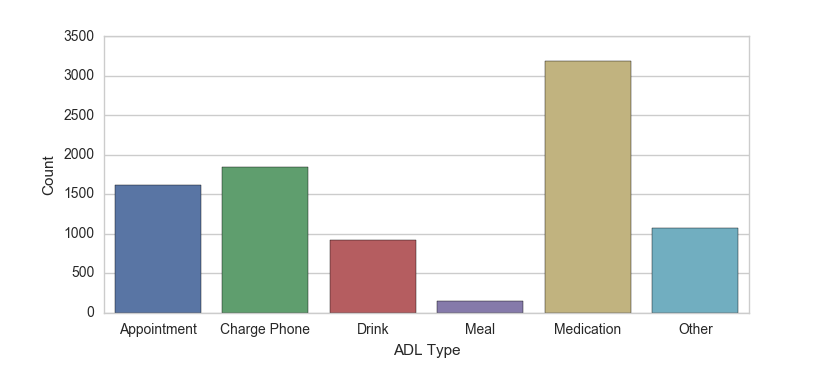
\includegraphics[scale=0.7, angle=0]{Files/treatment-study-1/figures/adl-type}
        \caption{Types of Acknowledged and Missed Reminders (n=8784) for DC participants.}
        \label{fig: adl-type}
\end{figure}


\section{Pre-Processing}
The proposed system should be able to regulate, through postponing or escalating, the delivery of reminders based on currently observed context states.
As such, the model will need to recognise the contexts which have had a historically high rate of acknowledgment, and those which have not. This can be performed via machine learning, by training a classifier, using each reminder's acknowledgement status as a class label.

To aid this step, the author developed a bespoke program\footnote{Source code available at: https://github.com/pjhartin/python-sensoranalysis-taut}, utilising the open source scientific tools provided in the \texttt{SciPy} and \texttt{NumPy} packages, to aid with the processing of the data generated within the app. The program was designed to pair, and label, the raw sensor data with the reminder data, validate the pairing, and facilitate the pre-processing, including filtering, windowing and feature extraction, of sensor data.

\subsection{Feature Selection}
Raw sensor data is varied and complex. It is, however, possible to derive a subset of values, or features, from the data which describe the data at a high level. Often these features are simple mathematical and statistical metrics, yet they describe the key characteristics of the signal.

Having demonstrated efficacy in all manner of classification problems \cite{Figo2010, Dargie2009, Bao2004}, the following 11 statistical features were calculated for each sensor recording in this study:

\begin{itemize}[noitemsep,topsep=0pt]
  \item Mean
  \item Median
  \item Minimum
  \item Max
  \item Variance
  \item Standard Deviation
  \item Root Mean Square
  \item Sum
  \item Range
  \item 75\% percentile cut-off
  \item 25\% percentile cut-off
\end{itemize}
% percentile cut offs?

In the example of accelerometer data, a 10 second sample, sampled at 100Hz, contains 10,000 values. A number of useful features can be selected from this sample, to describe the entire window of data. An example performed on two sample accelerometer signals is shown in Figure \ref{fig: feature-selection-example}. As such, it becomes very simple and efficient to compare multiple sensor recordings against one another based upon their features.

\begin{figure}[h]
    \centering
        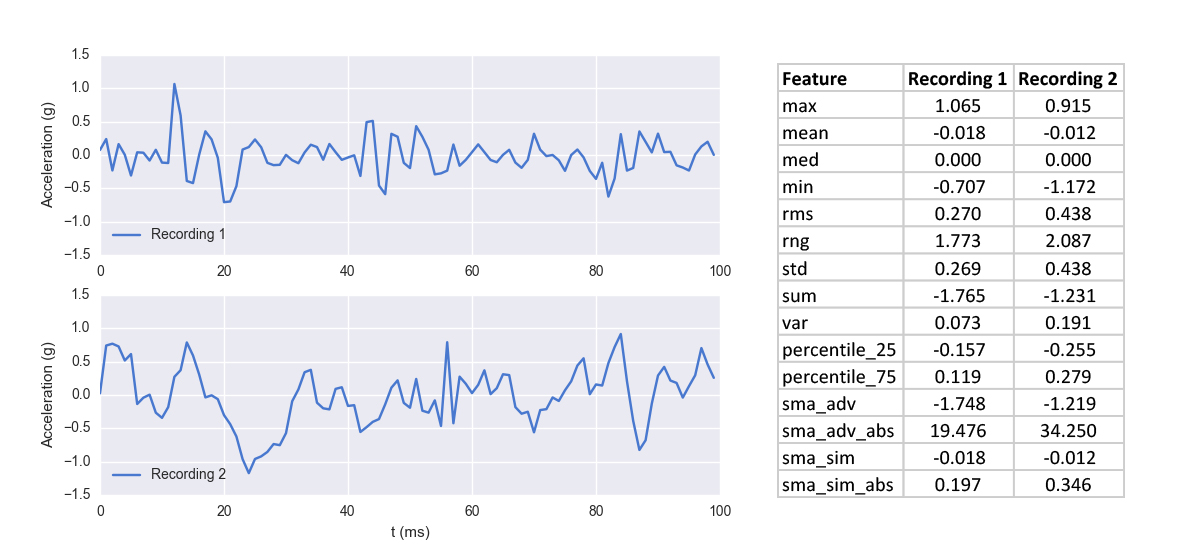
\includegraphics[scale=0.38, angle=0]{Files/treatment-study-1/figures/feature-selection-example}
        \caption{Example of feature selection performed on two similar accelerometer wave samples.}
        \label{fig: feature-selection-example}
\end{figure}

A key concept of the approach is that feature selection results in a set of relevant features, whilst removing redundant or irrelevant features which could negatively impact upon the accuracy of a classification model. The result is a set of features that are optimised to discriminate between the classes.
%VIVA: It is more that you are reducing the dimensionality of the problem as described by the feature vecore.  If this is reduced the classifier has an easier job at classifying the data.  The features assist in better discriminating between the classes.

\subsubsection{Signal Magnitude Area}
Multi-dimensional time-series data provides the opportunity to calculate additional features, such as the Signal Magnitude Area (SMA), as depicted in Equation \ref{eq: SMA},
\begin{equation}
SMA =\frac{1}{n} \left(\int_{0}^{n} \mid x(n)\mid \text{d} n + \int_{0}^{n} \mid y(n)\mid \text{d} n + \int_{0}^{n} \mid z(n)\mid \text{d} n  \right)
\label{eq: SMA}
\end{equation}
where $x$, $y$ and $z$ are the signals from each axis with respect to the sample number $n$, in a window.

The SMA has been used in studies as the basis to distinguish between periods of rest and activity \cite{Mathie2004, Karantonis2006}. The measure can be calculated in 2 ways:
\begin{description}
	\item [Simple] Calculated as simple sum of vector components, then normalised over length of the window.
	\item [Advanced] Calculated by subtracting the mean of the window from each of the axes to remove the average component
\end{description}

For thoroughness, both variations are calculated in this study when computing the SMA. In addition, the absolute values of both SMA variants are also recorded, resulting in 4 features per calculation.

\subsubsection{Frequency-Domain Analysis}
In similar works which aim to assess and quantify movement from accelerometers, frequency domain analysis has been used \cite{Preece2009}. The Fast Fourier Transform algorithm (FFT) \cite{Martens1992} has been frequently used in similar studies, after encouraging results were demonstrated by \citeauthor{Bao2004} for the classification of various movements in \citeyear{Bao2004} \cite{Bao2004}. The FFT transforms finite data, in this case windowed time-series data, into a spectrum of frequency components, showing their distribution. Additional features can be derived from the resulting data, by performing principal component analysis \cite{Preece2009} or extracting the energy spectrum \cite{Tapia2007}.
In previously published works by the author \cite{Hartin2014-WAGER}, the FFT algorithm was applied to windowed samples of both the accelerometer and the magnetometer signals. This application exposed limitations of the android platform for scientific application of FFTs. The android platform restricts a developer from explicitly setting a fixed sampling rate \cite{GoogleAndroid2016a}, resulting in inaccurate and incorrect frequency calculations. The cause is due to the variance in handset hardware. Since the Google Android platform cannot guarantee the hardware capabilities of each handset, the option to set the sampling rate (20Hz, 50Hz, 100Hz, etc.) or range (1.0g, 2.0g, 4.0g) is limited to choosing from a range of 4 options:

\begin{description}
	\item [\texttt{SENSOR\textunderscore DELAY\textunderscore UI}] suitable for the user interface
	\item [\texttt{SENSOR\textunderscore DELAY\textunderscore NORMAL}] suitable for screen orientation changes (default)
	\item [\texttt{SENSOR\textunderscore DELAY\textunderscore GAME}] suitable for games
	\item [\texttt{SENSOR\textunderscore DELAY\textunderscore FASTEST}] get sensor data as fast as possible
\end{description}

As such, in this study, the fastest option (\texttt{SENSOR\textunderscore DELAY\textunderscore FASTEST}) has been selected, which for the Motorola Moto G's hardware is 100Hz. This sampling rate, however, is still not guaranteed. The rate can vary due to processing and bandwidth bottlenecks on the device. As such, time to frequency transforms become computationally more expensive, especially on the device in real-time.

For these reasons, frequency domain features are not explored any further in this study.

\subsection{Summary of Features}
As the most promising features for the approach are yet to be established, the author employed a test-all approach, making use of all available features which have found successful application in other areas \cite{Figo2010}. In total, for each reminder instance, 330 features were calculated from the various sensors. These features are in-line with those typically used for context recognition from accelerometer data in similar studies \cite{Figo2010}.

\subsection{Processing Data Streams}
Although there are 4 sensors in the study, each sensor can provide a multitude of data streams, each of which can be processed further and used to create additional data sources. This sub-section will detail the data streams extracted from the sensors, and those created during processing.

\subsubsection{Multi-dimensional}
The accelerometer and magnetometer format their readings as a 4-dimensional array, consisting of time (t), and the 3-dimensions of space (x, y and z). Each individual dimension can be extracted from the array enabling a number of options for analysis. For example, it is possible to create a composite signal, by calculating the Signal Vector Magnitude (SVM) as described in Equation \ref{eq: SVM}.
\begin{equation}
SVM =\frac{1}{n} \sum_{i=1}^b \sqrt{x_i^2 + y_i^2 + z_i^2 }
\label{eq: SVM}
\end{equation}
where $x$, $y$ and $z$ are the signals from each axis with respect to the sample number $n$, in a window.

The SVM results in a single signal, which whilst losing a degree of fidelity, provides a good measure of the intensity of movement observed across all the axes \cite{Karantonis2006}. The SVM from accelerometry has been successfully utilised to classify various physical movements \cite{Gu2011,Banos2012,Pande2013}. In this study, the SVM is calculated for both the accelerometer and magnetometer signals, and used as an additional data source.


\subsubsection{Discrete Data}
The light and proximity sensors record their observations in a discrete manner in an effort to improve processing efficiency and battery life. When the sensor is first polled, a reading is taken. The sensor then polled at intervals checking for a change in value. If a value change is detected, the new value is recorded. This results in a 2 dimensional array, consisting of time and the observed value. An example of the discrete data imposed onto the continuous data observed from an accelerometer is presented in Table \ref{tbl: time-series-discretel}.

\begin{table}[h]
\centering
\caption{Example of continuous accelerometer series data and discrete sensor observations over time. Empty values for the discrete sensors assume the previously polled sensor value.}
\label{tbl: time-series-discretel}
\begin{tabular}{@{}ccccccc@{}}
\toprule
Time    & \multicolumn{4}{c}{Accelerometer} & Light        & Proximity    \\ \midrule
t    & x      & y      & z      & svm    & n            & n            \\ \midrule
1    & 1.245  & 0.569  & 10.042 & 4.772  & 65.12        & 5            \\
2    & 1.142  & 0.497  & 9.908  & 4.702  &              &              \\
3    & 1.218  & 0.511  & 9.810  & 4.704  &              &              \\
4    & 1.481  & 0.465  & 10.002 & 4.809  &              & 0            \\
5    & 1.285  & 0.566  & 9.832  & 4.738  &              &              \\
6    & 1.268  & 0.629  & 9.973  & 4.776  &              &              \\
7    & 1.299  & 0.624  & 10.015 & 4.792  &              & 5            \\
8    & 1.263  & 0.614  & 9.988  & 4.775  & 67.43        &              \\
9    & 1.315  & 0.533  & 10.041 & 4.783  &              &              \\
...  & ...    & ...    & ...    & ...    & ...          & ...          \\
t(i) & x(i)   & y(i)   & z(i)   & svm(i) & n(i) or last & n(i) or last \\ \bottomrule
\end{tabular}
\end{table}

\subsection{Filtering and Calibration}
Accelerometers and magnetometers found in smartphones are not designed to be high accuracy reference instruments. Often lower quality hardware is used, which results in noisy and uncalibrated signals \cite{Mitchell2013}. Despite this, smartphones are consistently used in scientific research due to their widespread prevalence and potential use cases. To counter the noise found in smartphone sensors, filtering is commonly applied to the signals.
%VIVA: Be prepared to discuss filtering during the VIVA!

\subsubsection{Filtering}
Having shown efficacy in similar studies \cite{Xia2011}, a median filter was chosen as an appropriate filter to remove noise from each signal. The median filter, when applied, transforms a list of values across a window length, based upon the median value for that window. The optimal size of the sliding-window depends upon the signal input and the desired level of smoothing.
To determine the appropriate size for this study, a number of tests were performed.

\textbf{Sliding Window-Length.}
Firstly a number of samples of missed and acknowledged reminders were chosen to study. For each recording the statistical features were extracted and recorded.
A range of window lengths (3-61) were then applied to the samples. From the resulting filtered signal, the same statistical features were calculated.
%VIVA: Why 3-61?
As the system aims to solve a binary classification problem (recognising acknowledged or missed), it was decided that the numerical difference between the features was key to a classifier's success. As such, a percentage difference comparison between the features of missed and acknowledged reminders was then performed for the raw and filtered data of various window lengths.
From the samples, the mean percentage difference between the classes (Acknowledged, Missed) for the unfiltered data, was 54\%, as seen in Figure \ref{fig: filter-percentage-difference} and Table \ref{tbl: percentage-difference-example}. Filtering the data using a median filter, with the minimum window length of 3 immediately improved the percentage difference observed. As presented in Figure \ref{fig: filter-percentage-difference}, increasing the window-length continues to widen the percentage difference in the features from the two classes.

\begin{figure}[]
    \centering
        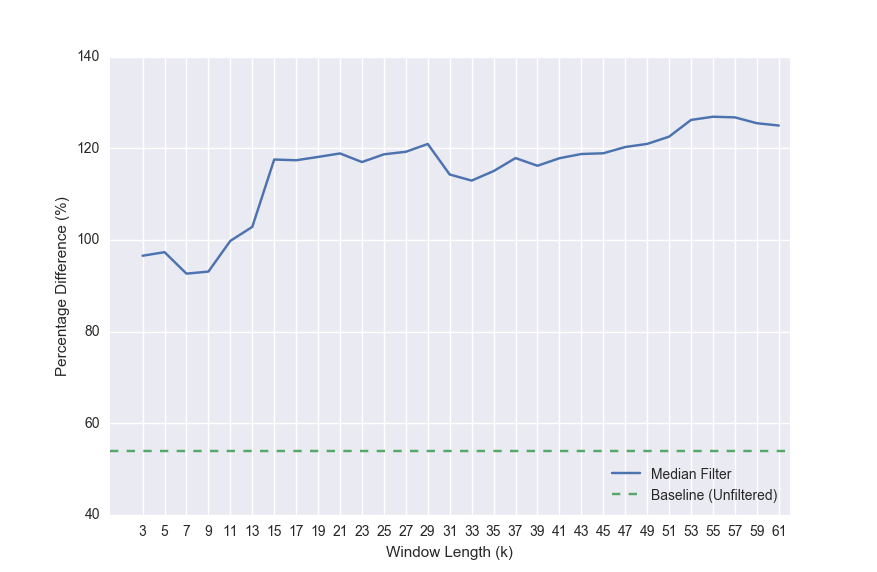
\includegraphics[scale=0.65, angle=0]{Files/treatment-study-1/figures/filter_window_length}
        \caption{Mean percentage difference observed between missed and acknowledged features for median filter window lengths.}
        \label{fig: filter-percentage-difference}
\end{figure}

At a window-length of 15, the difference reaches its first peak, after which, future improvement comes at computationally diminishing returns, eventually plateauing at the maximum of 61. An example of output from the process, using the observed optimal window-length of 15 for the median filter is shown in Table \ref{tbl: percentage-difference-example}.
%VIVA: Chris comment -  Has this been a subjective process if limited data has been used to define the window length.  I guess it is difficult to justify this either way.

\begin{table}[]
\centering
\caption{Comparison of extracted features and their percentage difference between classes in filtered and unfiltered data.}
\label{tbl: percentage-difference-example}
\resizebox{\textwidth}{!}{%
\begin{tabular}{@{}lllllll@{}}
 & \multicolumn{3}{c}{Raw (No Filter)} & \multicolumn{3}{c}{Median Filter (k=15)} \\ \midrule
Feature & Missed & Acknowledged & Difference (\%) & Missed & Acknowledged & Difference (\%) \\ \midrule
max & 31.4329 & 9.6185 & 106.28 & 0.2363 & 1.2724 & 137.35 \\
mean & 0.0610 & 0.0941 & 42.73 & 0.0052 & 0.0611 & 168.82 \\
min & -1.9669 & -3.0805 & 44.13 & -1.9682 & -0.5349 & 114.52 \\
percentile 25 & -0.1244 & -0.2036 & 48.32 & -0.0409 & -0.0912 & 76.13 \\
percentile\_75 & 0.1616 & 0.3051 & 61.47 & 0.0441 & 0.1988 & 127.34 \\
rms & 1.1788 & 0.7953 & 38.85 & 0.1065 & 0.2553 & 82.27 \\
rng & 33.3997 & 12.6991 & 89.81 & 2.2045 & 1.8073 & 19.80 \\
sma\_adv & 48.7090 & 75.1810 & 42.73 & 4.1303 & 48.8546 & 168.82 \\
sma\_adv\_abs & 232.7426 & 358.4968 & 42.54 & 50.1466 & 146.0025 & 97.74 \\
sma\_sim & 0.0610 & 0.0941 & 42.73 & 0.0052 & 0.0611 & 168.82 \\
sma\_sim\_abs & 0.2913 & 0.4487 & 42.54 & 0.0628 & 0.1827 & 97.74 \\
std & 1.1772 & 0.7897 & 39.40 & 0.1063 & 0.2478 & 79.90 \\
sum & 48.7700 & 75.2751 & 42.73 & 4.1354 & 48.9157 & 168.82 \\
var & 1.3858 & 0.6236 & 75.85 & 0.0113 & 0.0614 & 137.80 \\ \midrule
Mean & - & - & 54.29 & - & - & 117.56 \\ \bottomrule
\end{tabular}
}
\end{table}

The median filter with a window-length of 15 provides an inexpensive method of filtering a signal, and displays efficiency in removing outliers whilst retaining detail. An example of this can be found in Figure \ref{fig: apply-filter}, where a recording from the study displays noise and artificial spikes in the data.

\begin{figure}[h]
    \centering
        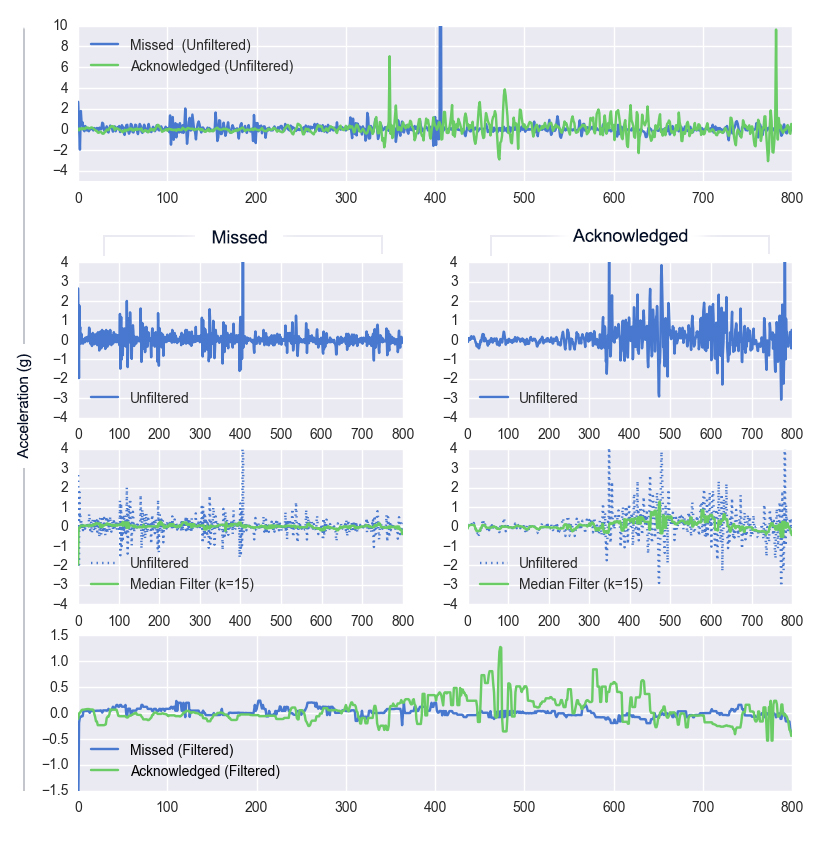
\includegraphics[scale=0.5, angle=0]{Files/treatment-study-1/figures/filtering_figure}
        \caption{Application of median filter (k=15) to accelerometer data. Resultant signal shows removal of noise, making the difference in each waveform more prominent.}
        \label{fig: apply-filter}
\end{figure}


\subsubsection{Calibration}
In addition to filtering, calibration was performed on the accelerometer and magnetometer data. Correctly performed, calibration enables all the recordings to have the same point of reference, resulting in precise, accurate and valid comparisons.
Whilst rudimentary calibration can be performed in the field \cite{Ferraris1995}, it requires a level of user input and knowledge which the author did not wish to ask of the end-users with dementia. The author also did not have any physical access to the handsets prior to deployment, and as a result, could not guarantee the devices were calibrated accurately.
Initial screening of the recorded data from various users uncovered that accelerometer readings were offset to various degrees depending on the device. Whilst this is a non-issue when comparing data from the same device as the offset is shared amongst all the recordings, the lack of calibration makes comparison with data observed from another device less valid.
To address this issue, for each SVM signal, the signal was reproduced, with an offset set as the median value of the signal. This rudimentary method resulted in a SVM which was effectively calibrated to 0, whilst maintaining the same shape and features, allowing much more accurate comparisons across devices.
%VIVA: Chris - Have you any references to support this approach?  I suspect this will be discussed at the viva
%VIVA: P - Whilst such an approach on live streaming data would be counter productive and drastically skew any data observed, having the entire of 6 minutes gave a large range of data from which to establish the true median value, or x-intercept.

\subsection{Windowing}
Although each sensor recording is 6 minutes in duration, the resulting system aims to \textit{predict} if a reminder will be acknowledged or missed. therefore only data observed before the reminder was delivered can be used.
The immediate point of reminder delivery is selected as the cutoff point in the signal, a figure which is extracted from the reminder log data, as illustrated in Figure \ref{fig: accelerometer-full-windowed}.

\begin{figure}[h]
    \centering
        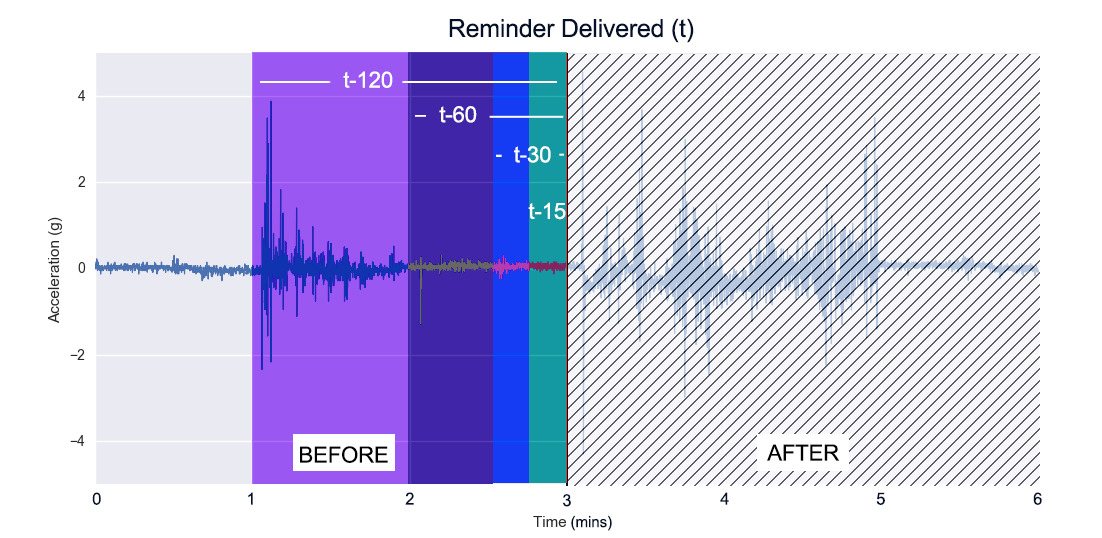
\includegraphics[scale=0.35, angle=0]{Files/treatment-study-1/figures/accelerometer-full-windowed}
        \caption{Illustration of signal windowing, with window endpoint as time of reminder delivery (t), and start point calculated by subtracting the desired window lengths (t-k).}
        \label{fig: accelerometer-full-windowed}
\end{figure}

The resulting signal is approximately 3 minutes long, and contains only the sensors readings \textit{prior} to the reminder being issued.
To establish an appropriate window length, a range of values were tested (10, 15, 20, 30 seconds). Whilst smaller windows, in the order of 1-5 seconds, have been shown to be useful in the recognition of different physical activities \cite{Wagenaar2011, Khan2014}, preliminary testing suggested that for this application, measurements extracted from larger windows provided greater distinguishing features. It is from these windows that the features were extracted.

\subsection{Labelling}
Using the acknowledgement data generated from each reminder delivery, it is possible to label each feature as acknowledged or missed for the purposes of training and validation within the supervised machine-learning phase.

\subsection{Classification}
Once all the features have been selected and labelled for their respective classes, the data is ready to be used to build a classifier. In this study, the Waikato Environment for Knowledge Analysis (Weka)  machine learning and experimentation suite \cite{Hornik2009} was used as the primary tool for the development of classification models. Weka provides a number of classification and modeling algorithms commonly used in context-aware applications, including:
\begin{description}[noitemsep,topsep=0pt]
	\item [J48] A C4.5 decision tree learner
	\item [NaiveBayes] A Naive Bayesian learner.
	\item [Logistic] Logistic Regression.
	\item [SMO] A Support Vector Machine (linear, polynomial and RBF kernel)
	\item [KStar] Instance-Based learner.
	\item [IBk] Instance-Based nearest neighbour learner with fixed neighbourhood.
	\item [JRip] A clone of the RIPPER rule learner.
\end{description}

As no single classifier family has had a distinct advantage in context or activity classification problems \cite{Mitchell2013a}, the author examined all possible options provided by the Weka tool. In each case, a classifier's performance is benchmarked against the ZeroR classifier, which predicts the modal, or majority, class for all future instances. E.g., for a data set of 60 instances of Class A, and 40 instances of Class B, the ZeroR classifier will classify all new instances as the most frequently occurring class (Class A), resulting in an baseline accuracy of 60\%.

\subsubsection{Measures of Comparison}
Accuracy, when used as the main metric of comparison can be a misleading representation of a classifiers performance. In addition to the accuracy (percentage correct), the sensitivity (precision), specificity (recall), Kappa statistic and the Area Under the ROC curve are also considered in the comparison of results.

\textbf{Sensitivity.}
The sensitivity, or precision, of a classifier is the proportion of instances that were truly of a class divided by the total instances classified as that class.

\textbf{Specificity.}
The specificity, or recall, of the classifier is the proportion of instances classified as a given class divided by the actual total in that class. This is also equivalent to True Positive rate.
%VIVA: Understand precision and recall?

\textbf{F-Measure.} The F-Measure is a combined measure for precision and recall, giving the mean for equally weighted measures.

\textbf{Kappa Statistic.}
The kappa statistic is a valuable measure to compare classifiers amongst themselves. The statistic is the result of the comparison between the observed accuracy of the classifier, with an expected accuracy, obtained through random chance. An advantage of using the kappa statistic to compare classifiers is the ability to categorise into performance groups, such as those proposed by \citeauthor{Landis1977}: 0-0.20 as slight, 0.21-0.40 as fair, 0.41-0.60 as moderate, 0.61-0.80 as substantial, and 0.81-1 as almost perfect \cite{Landis1977}.

\textbf{Area Under Curve (ROC).}
The Area Under Curve metric measures the performance of a binary classification. When used in a regression classification for a binary class problem, it is possible to plot the probability threshold changes in an ROC curve \cite{Metz1978}. This curve plots the True Positive rate against the False positive rate. An example ROC graph is presented in Figure \ref{fig: auc-roc-example}.

\begin{figure}[h]
    \centering
        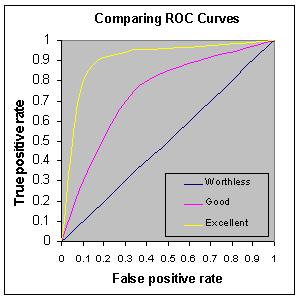
\includegraphics[scale=3, angle=0]{Files/treatment-study-1/figures/auc-roc-example}
        \caption{Illustration of Area Under an ROC including example ratings of model fit. Image Source: \fullcite{Tape} \cite{Tape}.}
        \label{fig: auc-roc-example}
\end{figure}

The graph essentially shows that given a random class A and class B observation, the area under the curve gives the proportion of correct guesses. The area under the ROC curve (AUC) is much less affected by the sample balance than the accuracy metric. To understand the rankings of the metric, a perfect model has an area of 1, whilst purely random is 0.5.
Medical practitioners using the AUC suggest the following classifications for the models fit \cite{Tape}:
\begin{itemize}[noitemsep,topsep=0pt]
  \item \textgreater .90 - Outstanding
  \item .80-.90 - Excellent (Good)
  \item .70-.80 - Acceptable (Fair)
  \item .60-.70 - Poor
  \item .50-.60 - No Discrimination
\end{itemize}

\subsection{Overview}
The order of the process is displayed in Figure \ref{fig: process-overview}. Raw sensor data is downloaded from the device, paired with reminder data, windowed, filtered, and features are extracted from both filtered and non-filtered data. The features are then appended to a list, and exported to external file system as both a labelled csv file, and a Weka formatted arff file.

\begin{figure}[h]
    \centering
        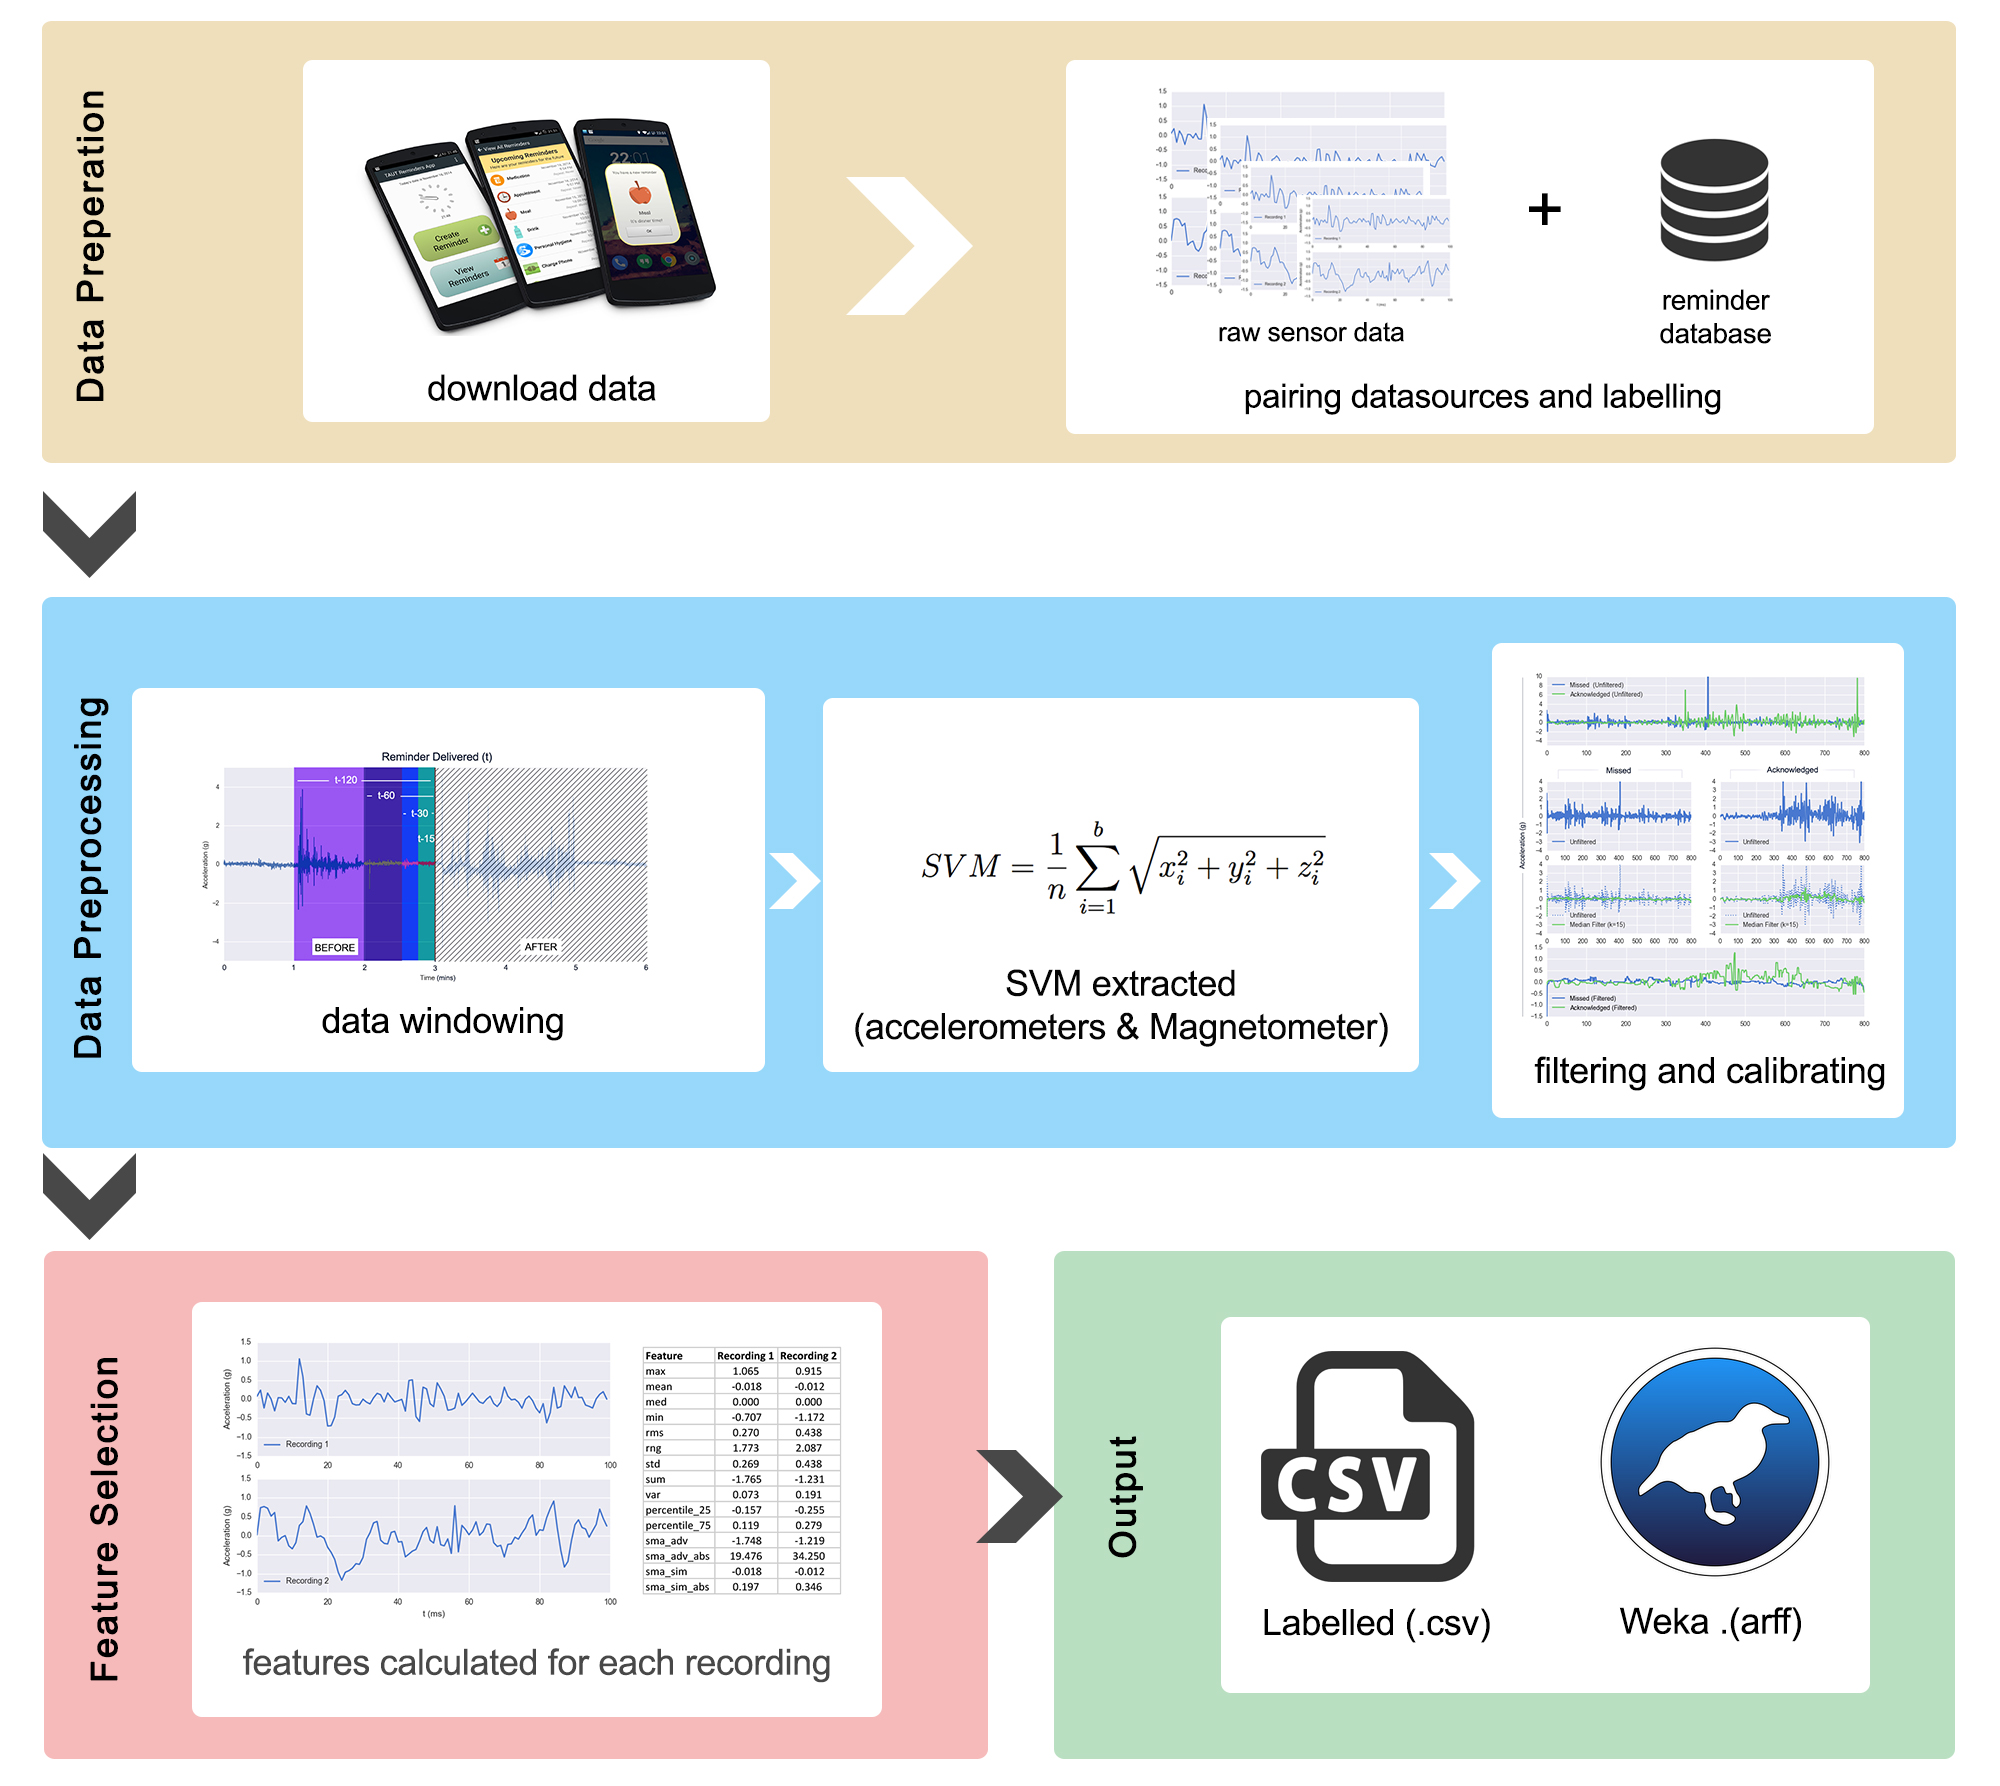
\includegraphics[scale=0.2, angle=0]{Files/treatment-study-1/figures/process-outlined}
        \caption{Illustration of procedure, from data collection, to pre-processing, feature selection, and output.}
        \label{fig: process-overview}
\end{figure}

\section{Results} \label{section: taut-results}
This Section details the results from the application of various classifiers to the resulting datasets of the TC and DC studies. In addition, the application of ensemble methods and data balancing are also explored, along with the evaluation of personalised models.

\subsection{Generalised Model}
Combining the data from all the participants in each study, respectively, resulted in 2 large datasets. These datasets were subsequently used in an effort to create a generalised model to predict missed or acknowledged reminder contexts. The data from the DC is explored first, and later contrasted to the TC data.

\subsubsection{Base Accuracy}
From the pre-processing stage a multitude of datasets were output for each window length (15, 20, 30, 45, 60, 90 seconds). Each dataset was analysed independently in an attempt to establish the optimal window length and classifier choice for future analysis. This was performed by applying a range of classifiers to the various windowed datasets. The results are presented in Table \ref{tbl: base-accuracy-windows}. Note that KStar (K*), an instance based-classifier, was removed from the analysis due to poor performance in the development of a generalised model in previous works by the author \cite{Hartin2014-WAGER}.

\begin{table}[h]
\centering
\caption{Accuracy (\%) of classifiers tested for numerous window lengths, showing statistically significant improvement and degradation over base ZeroR classifier at the p \textless .05 level.}
\label{tbl: base-accuracy-windows}
\resizebox{\textwidth}{!}{%
\begin{tabular}{@{}llllllllllllll@{}}
\toprule
\begin{tabular}[c]{@{}l@{}}Window\\ Size\end{tabular} & \begin{tabular}[c]{@{}l@{}}ZeroR\\ (Base)\end{tabular} & J48 &  & \begin{tabular}[c]{@{}l@{}}Naive \\ Bayes\end{tabular} &  & Logistic &  & SMO &  & IBK &  & JRip &  \\ \midrule
15s & 72.84 & 80.31 & $\circ$ & 53.17 & $\bullet$ & 78.26 & $\circ$ & 76.27 & $\circ$ & 51.24 & $\bullet$ & 81.14 & $\circ$ \\
20s & 72.84 & 81.23 & $\circ$ & 51.56 & $\bullet$ & 78.86 & $\circ$ & 76.47 & $\circ$ & 55.62 & $\bullet$ & 81.60 & $\circ$ \\
30s & 72.84 & 79.93 & $\circ$ & 52.19 & $\bullet$ & 79.27 & $\circ$ & 76.38 & $\circ$ & 54.61 & $\bullet$ & 81.83 & $\circ$ \\
45s & 72.84 & 79.64 & $\circ$ & 52.05 & $\bullet$ & 79.67 & $\circ$ & 76.47 & $\circ$ & 57.09 & $\bullet$ & 81.75 & $\circ$ \\
60s & 72.84 & 81.29 & $\circ$ & 52.11 & $\bullet$ & 79.30 & $\circ$ & 76.50 & $\circ$ & 56.92 & $\bullet$ & 81.57 & $\circ$ \\
90s & 72.84 & 79.70 & $\circ$ & 52.22 & $\bullet$ & 78.95 & $\circ$ & 76.38 & $\circ$ & 55.97 & $\bullet$ & 81.66 & $\circ$ \\ \midrule
\multicolumn{14}{c}{$\circ$, $\bullet$ statistically significant improvement or degradation at the p\textless .05 level} \\ \bottomrule
\end{tabular}
}
\end{table}

Looking at rest of data, decision tree and rule-based classifiers, J48 and JRip, are performing the best. A window size of 30s provided the best performance for JRip, whilst 20s was best for J48. Analysis of the other comparison measures between these window sizes can be found in Table \ref{fig: window-length-measure-comparison}.

\begin{table}[h]
\centering
\caption{Comparison of classification performance measures for 20 and 30 second window lengths.}
\label{fig: window-length-measure-comparison}
\resizebox{\textwidth}{!}{%
\begin{tabular}{@{}llllllllll@{}}
\toprule
Measure & \begin{tabular}[c]{@{}l@{}}Window\\ Length\end{tabular} & \begin{tabular}[c]{@{}l@{}}ZeroR \\ (Base)\end{tabular} & J48 & \begin{tabular}[c]{@{}l@{}}Naive \\ Bayes\end{tabular} & Logistic & SMO & IBk & JRip & Mean \\ \midrule
\multirow{2}{*}{Precision} & 20 & 0 & 0.66 & 0.34 & 0.66 & 0.8 & 0.35 & 0.68 & 0.58 \\
 & 30 & 0 & 0.63 & 0.35 & 0.66 & 0.77 & 0.35 & 0.68 & 0.57 \\ \midrule
\multirow{2}{*}{Recall} & 20 & 0 & 0.64 & 0.86 & 0.46 & 0.18 & 0.71 & 0.61 & 0.58 \\
 & 30 & 0 & 0.63 & 0.89 & 0.48 & 0.19 & 0.75 & 0.64 & 0.60 \\ \midrule
\multirow{2}{*}{F-Measure} & 20 & 0 & 0.65 & 0.49 & 0.54 & 0.29 & 0.47 & 0.64 & 0.51 \\
 & 30 & 0 & 0.63 & 0.5 & 0.56 & 0.3 & 0.47 & 0.65 & 0.52 \\ \midrule
\multirow{2}{*}{Kappa} & 20 & 0 & 0.52 & 0.16 & 0.41 & 0.22 & 0.16 & 0.52 & 0.33 \\
 & 30 & 0 & 0.49 & 0.18 & 0.43 & 0.22 & 0.16 & 0.53 & 0.34 \\ \midrule
\multirow{2}{*}{ROC} & 20 & 0.5 & 0.78 & 0.64 & 0.79 & 0.58 & 0.61 & 0.76 & 0.69 \\
 & 30 & 0.5 & 0.77 & 0.64 & 0.8 & 0.58 & 0.61 & 0.77 & 0.70 \\ \bottomrule
\end{tabular}
}
\end{table}

From the Table, it is clear that the differences between the two window sizes are extremely small. In all measures, with the exception of precision, the 30 second window size performs marginally better. As such, all future analysis was performed on the data derived from the 30 second window.

\subsubsection{Ensemble Methods}
Whilst the J48 (79.93\%) and JRip (81.83\%) classifiers were performing statistically significantly better than a majority classifier (72.84\%), there are still a number of ways in which to further boost the performance of the models. Identified as one of the top 10 algorithms in data mining by \citeauthor{Wu2007} \cite{Wu2007}, ensemble methods such as boosting, bagging and blending (or stacking) can improve classification performance in a myriad of tasks, and are especially useful when dealing with C4.5 decision trees (J48).

\textbf{Boosting.}
Boosting uses a base classifier to build a model based upon the training data, after which, a second classifier is then created to focus on the instances that the first classifier predicted incorrectly. The process continues until a limit of models or accuracy is achieved.

\textbf{Bagging.}
Bagging creates separate training samples from the original dataset, and creates a classifier for each sample. Through averaged or majority voting the results of the classifiers are combined to create a base classifier. This methods strength is based on the premise that the separate training samples have subtly unique perspectives on the classification problem. 

\textbf{Blending.}
Blending, or stacking, involves using multiple different classification algorithms to prepare a model on the training data. After which, a combiner algorithm, or meta-classifier, is trained to make the final prediction, using the predictions of the other classifiers as inputs.

As the J48 and JRip algorithms performed best on the data in the previous section, J48 was used as the base classifier for both boosting and Bagging, and a combination of J48 and JRip were used for the Blending (Stacking) algorithm. Each was applied to the DC's data, and the results compared against the J48 (C4.5 decision tree) from the previous section. Full results are displayed in Table \ref{tbl: utah-ensemble-results}. The application of Bagging (J48) and Blending (J48 with JRip) resulted in significant improvement in accuracy, precision and ROC over the base J48, whilst significantly decreasing recall. In this case, the decrease in recall (True Positive Rate) is the ability to correctly identify a context in which acknowledgements occurred. An ROC of over .8, as found with the ensemble methods would be considered an excellent fit by the guidelines outlined in \cite{Tape}.

\begin{table}[h]
\centering
\caption{Results of ensemble classifiers applied to DC dataset, showing statistical significance against J48 (C4.5 Decision Tree) as base comparison.}
\label{tbl: utah-ensemble-results}
\resizebox{\textwidth}{!}{%
\begin{tabular}{@{}llllllllllll@{}}
\toprule
Measure & \begin{tabular}[c]{@{}l@{}}J48 \\ (Base)\end{tabular} & ZeroR &  & JRip &  & \begin{tabular}[c]{@{}l@{}}Boosting \\ (J48)\end{tabular} &  & \begin{tabular}[c]{@{}l@{}}Bagging \\ (J48)\end{tabular} &  & \begin{tabular}[c]{@{}l@{}}Blending \\ (J48/JRip)\end{tabular} &  \\ \midrule
Accuracy (\%) & 79.93 & 72.84 & $\bullet$ & 81.83 &  & 78.69 &  & 81.89 & $\circ$ & 81.92 & $\circ$ \\
Precision & 0.63 & 0 & $\bullet$ & 0.68 & $\circ$ & 0.62 &  & 0.71 & $\circ$ & 0.71 & $\circ$ \\
Recall & 0.63 & 0 & $\bullet$ & 0.64 &  & 0.57 & $\bullet$ & 0.57 & $\bullet$ & 0.56 & $\bullet$ \\
F-Measure & 0.63 & 0 & $\bullet$ & 0.65 &  & 0.59 & $\bullet$ & 0.63 &  & 0.62 &  \\
Kappa & 0.49 & 0 & $\bullet$ & 0.53 &  & 0.45 &  & 0.51 &  & 0.51 &  \\
ROC & 0.77 & 0.5 & $\bullet$ & 0.77 &  & 0.82 & $\circ$ & 0.85 & $\circ$ & 0.82 & $\circ$ \\ \midrule
\multicolumn{12}{c}{$\circ$, $\bullet$ statistically significant improvement or degradation at the p\textless .05 level} \\ \bottomrule
\end{tabular}
}
\end{table}

\subsubsection{Balancing the Dataset}
Whilst the ensemble methods did improve the classification performance, it was apparent that the classes (Acknowledged/Missed) were not represented equally in the data, and as such any model built upon the training data will be imbalanced to the majority class. Imbalance in datasets is common, and in this case, was expected. The ratio of Missed (n=2562) to Acknowledged (n=942) reminders is almost 35:13 (421:157 Simplified). To balance the training dataset to 50:50 (Kappa = 0) a number of methods may be used which may be referred to as stratification.

\textbf{Resampling.}
Resampling is performed by simply replicating instances of the minority class back into the training set until the distribution is equal. 

\textbf{Downsampling.}
Downsampling is the opposite approach, and involves removing instances from the majority class, so that the distribution is equal. 

Both of these methods bring distinct disadvantages, namely overfitting to the minority class in resampling, and losing truth and variance in downsampling. An ideal and optimal approach is the use of synthetic data \cite{nonnemaker2008}.

\textbf{Synthetic Data.} The generation of synthetic data based on the minority class is a method of balancing the dataset. The most popular of such algorithms is the Synthetic Minority Over-sampling Technique (SMOTE). SMOTE functions by selecting a number of instances, and randomly alters the data one attribute at a time within a neighbouring difference of the selected instances. This results in the creation of additional instances that are similar, through statistical methods, however, not exact copies of instances from the same class \cite{Chawla2011}. SMOTE has been applied to many binary classification problems to help balance datasets across various research fields including pharmacology \cite{Kumari2015}, oncology \cite{Fehr2015}, information science \cite{Cleland2014-IWAAL, Zhang2013}, and even radar ornithology \cite{D.Rosa2016}.

Having applied SMOTE to the minority class (Acknowledged) to an effect of 168.16\%, resulted in a balanced dataset of 2526:2526 reminders.  
The same classifiers and ensemble methods were applied to the balanced dataset. Again, the basic J48 was used as the base of comparison for statistical significance tests between the classifiers as shown in Table \ref{tbl: utah-smote-classifiers}. In addition, comparisons between the datasets measures was also performed, as presented in Table \ref{tbl: utah-smote-dataset}.

\begin{table}[h]
\centering
\caption{Comparison of classifier performances on unbalanced dataset and SMOTE balanced dataset.}
\label{tbl: utah-smote-classifiers}
\resizebox{\textwidth}{!}{%
\begin{tabular}{@{}lllllllllllll@{}}
\toprule
Measure & Dataset & \begin{tabular}[c]{@{}l@{}}J48 \\ (Base)\end{tabular} & ZeroR &  & JRip &  & \begin{tabular}[c]{@{}l@{}}Boosting\\ (J48)\end{tabular} &  & \begin{tabular}[c]{@{}l@{}}Bagging\\ (J48)\end{tabular} &  & \begin{tabular}[c]{@{}l@{}}Blending \\ (J48/JRip)\end{tabular} &  \\ \midrule
\multirow{2}{*}{Accuracy (\%)} & Imbalanced & 79.93 & 72.84 & $\bullet$ & 81.83 &  & 78.69 &  & 81.89 & $\circ$ & 81.92 & $\circ$ \\
 & SMOTE & 78.31 & 50 & $\bullet$ & 80.07 &  & 82.98 & $\circ$ & 79.83 &  & 79.57 &  \\ \midrule
\multirow{2}{*}{F-Measure} & Imbalanced & 0.63 & 0 & $\bullet$ & 0.65 &  & 0.59 & $\bullet$ & 0.63 &  & 0.62 &  \\
 & SMOTE & 0.77 & 0 & $\bullet$ & 0.78 &  & 0.83 & $\circ$ & 0.78 &  & 0.79 &  \\ \midrule
\multirow{2}{*}{Kappa} & Imbalanced & 0.49 & 0 & $\bullet$ & 0.53 &  & 0.45 &  & 0.51 &  & 0.51 &  \\
 & SMOTE & 0.57 & 0 & $\bullet$ & 0.6 &  & 0.66 & $\circ$ & 0.6 &  & 0.59 &  \\ \midrule
\multirow{2}{*}{Precision} & Imbalanced & 0.63 & 0 & $\bullet$ & 0.68 & $\circ$ & 0.62 &  & 0.71 & $\circ$ & 0.71 & $\circ$ \\
 & SMOTE & 0.82 & 0 & $\bullet$ & 0.84 &  & 0.81 &  & 0.84 & $\circ$ & 0.82 &  \\ \midrule
\multirow{2}{*}{Recall} & Imbalanced & 0.63 & 0 & $\bullet$ & 0.64 &  & 0.57 & $\bullet$ & 0.57 & $\bullet$ & 0.56 & $\bullet$ \\
 & SMOTE & 0.73 & 0 &  & 0.74 &  & 0.86 & $\circ$ & 0.74 &  & 0.76 &  \\ \midrule
\multirow{2}{*}{ROC} & Imbalanced & 0.77 & 0.5 & $\bullet$ & 0.77 &  & 0.82 & $\circ$ & 0.85 & $\circ$ & 0.82 & $\circ$ \\
 & SMOTE & 0.85 & 0.5 & $\bullet$ & 0.82 &  & 0.9 & $\circ$ & 0.91 & $\circ$ & 0.89 & $\circ$ \\ \midrule
 \multicolumn{13}{c}{$\circ$, $\bullet$ statistically significant improvement or degradation at the p \textless .05 level} \\ \bottomrule
\end{tabular}
}
\end{table}

\begin{table}[ph]
\centering
\caption{Comparison of measures between unbalanced and balanced (SMOTE) DC dataset}
\label{tbl: utah-smote-dataset}
\begin{tabular}{@{}lllll@{}}
\toprule
Measure                    & Classifier          & \begin{tabular}[c]{@{}l@{}}Utah \\ (Original)\end{tabular}  & \begin{tabular}[c]{@{}l@{}}Utah \\ (SMOTE)\end{tabular} &         \\ \midrule
\multirow{6}{*}{Accuracy (\%)}  & JRip                & 81.83 & 80.07                                                   &         \\
                           & J48                 & 79.93 & 78.31                                                   &         \\
                           & Boosting (J48)      & 78.69 & 82.98                                                   & $\circ$ \\
                           & Bagging  (J48)      & 81.89 & 79.83                                                   &         \\
                           & Blending (J48/JRip) & 81.92 & 79.57                                                   &         \\
                           & Average             & 79.52 & 75.11                                                   &         \\ \midrule
\multirow{6}{*}{Precision} & JRip                & 0.68  & 0.84                                                    & $\circ$ \\
                           & J48                 & 0.63  & 0.82                                                    & $\circ$ \\
                           & Boosting (J48)      & 0.62  & 0.81                                                    & $\circ$ \\
                           & Bagging  (J48)      & 0.71  & 0.84                                                    & $\circ$ \\
                           & Blending (J48/JRip) & 0.71  & 0.82                                                    & $\circ$ \\
                           & Average             & 0.56  & 0.74                                                    &         \\ \midrule
\multirow{6}{*}{Recall}    & JRip                & 0.64  & 0.74                                                    &         \\
                           & J48                 & 0.63  & 0.73                                                    &         \\
                           & Boosting (J48)      & 0.57  & 0.86                                                    & $\circ$ \\
                           & Bagging  (J48)      & 0.57  & 0.74                                                    & $\circ$ \\
                           & Blending (J48/JRip) & 0.56  & 0.76                                                    & $\circ$ \\
                           & Average             & 0.49  & 0.74                                                    &         \\ \midrule
\multirow{6}{*}{F-Measure} & JRip                & 0.65  & 0.78                                                    & $\circ$ \\
                           & J48                 & 0.63  & 0.77                                                    & $\circ$ \\
                           & Boosting (J48)      & 0.59  & 0.83                                                    & $\circ$ \\
                           & Bagging  (J48)      & 0.63  & 0.78                                                    & $\circ$ \\
                           & Blending (J48/JRip) & 0.62  & 0.79                                                    & $\circ$ \\
                           & Average             & 0.52  & 0.72                                                    &         \\ \midrule
\multirow{6}{*}{Kappa}     & JRip                & 0.53  & 0.6                                                     &         \\
                           & J48                 & 0.49  & 0.57                                                    &         \\
                           & Boosting (J48)      & 0.45  & 0.66                                                    & $\circ$ \\
                           & Bagging  (J48)      & 0.51  & 0.6                                                     &         \\
                           & Blending (J48/JRip) & 0.51  & 0.59                                                    & $\circ$ \\
                           & Average             & 0.42  & 0.5                                                     &         \\ \midrule
\multirow{6}{*}{ROC}       & JRip                & 0.77  & 0.82                                                    & $\circ$ \\
                           & J48                 & 0.77  & 0.85                                                    & $\circ$ \\
                           & Boosting (J48)      & 0.82  & 0.9                                                     & $\circ$ \\
                           & Bagging  (J48)      & 0.85  & 0.91                                                    & $\circ$ \\
                           & Blending (J48/JRip) & 0.82  & 0.89                                                    & $\circ$ \\
                           & Average             & 0.75  & 0.81                                                    &         \\ \midrule
\multicolumn{5}{c}{$\circ$, $\bullet$ statistically significant improvement or degradation at the p \textless .05 level} \\ \bottomrule
\end{tabular}
\end{table}

The application of the SMOTE algorithm resulted in an improvement in almost every measurement for each classifier. The best improvements can be found in the recall and ROC of the boosting, bagging and blending ensemble methods. Recall, a previous weak point of the system has now been improved substantially, resulting in an ROC of .91 (outstanding) in the bagging method.

\subsubsection{Feature Evaluation}
Whilst the classifier was generated using a dataset which contained 330 features, it is highly likely that only a limited number of these were used. It is possible to rank the importance of these features in the classifier, exposing features which have been calculated, yet are redundant to the model. Identifying these features and removing them, will optimise the speed at which features are calculated for the model, an important step if the features are to be eventually calculated on the device.

Using a forward traversing, greedy, best first search algorithm, and evaluation performed on a 5-fold J48 decision tree, the 330 features were reduced to 8 by the Weka software package:
\begin{description}[noitemsep,topsep=0pt]
	\item [accelerometer\textunderscore y\textunderscore rng] Range observed in the acceleration on the Y axis
	\item [accelerometer\textunderscore z\textunderscore median \textunderscore filter \textunderscore med] Median value of the accelerometer's filtered Z axis
	\item [light\textunderscore measure\textunderscore min] Minimum value observed from the light sensor
	\item [magnetic\textunderscore x\textunderscore median\textunderscore filter\textunderscore std] Standard deviation of the magnetometers filtered X axis
	\item [magnetic\textunderscore y\textunderscore median\textunderscore filter\textunderscore percentile\textunderscore 25] Cutoff of the 25th percentile of the magnetometers filtered Y axis
	\item [magnetic\textunderscore y\textunderscore median\textunderscore filter\textunderscore std] Standard deviation of magnetometer's filtered Y Axis
	\item [magnetic\textunderscore y\textunderscore percentile\textunderscore 25] Cutoff of the 25th percentile of the magnetometers raw Y axis
	\item [proximity\textunderscore measure\textunderscore min] Minimum observed value of the proximity sensor
\end{description}

As presented in Table \ref{tbl: utah-8-features}, whilst using only 8 features, the accuracy of the results improved substantially for the all classifiers on the unbalanced dataset (Original statistics in Table \ref{tbl: utah-ensemble-results}), whilst simultaneously reducing the build time from 99 seconds to 0.08 seconds. Note the 8 features still span all four sensor modalities provided by the smartphone. 

\begin{table}[h]
\centering
\caption{Statistics for classifiers trained and tested using reduced feature set (n=8), established through J48 evaluated Best First search. Dataset was original unbalanced.}
\label{tbl: utah-8-features}
\begin{tabular}{@{}lllllll@{}}
\toprule
Measure   & \begin{tabular}[c]{@{}l@{}}ZeroR \\ (Base)\end{tabular} & Jrip  & J48  & \begin{tabular}[c]{@{}l@{}}Boosting \\ (AdaBoost - J48)\end{tabular} & \begin{tabular}[c]{@{}l@{}}Bagging \\ (J48)\end{tabular} & \begin{tabular}[c]{@{}l@{}}Blending \\ (J48/JRip)\end{tabular} \\ \midrule
Accuracy  & 72.84                                                   & 83.13 & 83.1 & 80.39                                                                & 83.62                                                    & 83.04                                                          \\
Precision & 0                                                       & 0.7   & 0.71 & 0.65                                                                 & 0.73                                                     & 0.72                                                           \\
Recall    & 0                                                       & 0.67  & 0.63 & 0.6                                                                  & 0.62                                                     & 0.61                                                           \\
F-Measure & 0                                                       & 0.68  & 0.67 & 0.62                                                                 & 0.67                                                     & 0.66                                                           \\
Kappa     & 0                                                       & 0.57  & 0.56 & 0.49                                                                 & 0.56                                                     & 0.55                                                           \\
ROC       & 0.5                                                     & 0.79  & 0.82 & 0.83                                                                 & 0.85                                                     & 0.83                                                           \\ \bottomrule
\end{tabular}
\end{table}

\subsection{Comparison with Preliminary}
Whilst the results are promising with the data gathered from the DC, it is worthwhile to compare with the data gathered from the TC, described earlier in the Chapter. The TC cohort had a very different ratio of acknowledged to missed reminders, 90:16 (Acknowledged: Missed). To ensure fair comparison the same method of oversampling using SMOTE and applying ensemble classifiers was applied to the TC's dataset. SMOTE was applied to the minority case, which in the TC was the missed reminder class, to the effect of 462.5\%. The results from each ensemble method were compared between the DC(SMOTE) and TC(SMOTE) datasets and the results are shown in Table \ref{tbl: smote-compare-dc-tc}. No significant differences were found in the results of either dataset, suggesting that the generalised approach is a good method for both cohorts. In addition the ROC model fit classification for the DC and TC averaged at Outstanding (.9) and Excellent (.83), respectively. In the interest of fully exploring the data, the DC dataset (n = 3469) was used as the training set, and tested on the TC dataset (n = 106) using the strongest performing classifier tested in the study (Bagging using J48). The training and testing split in this case was 96.5\%:3.5\% (5052:180).
The resulting accuracy of the model was only 66\% (F-Measure 0.651), showing that each cohorts data were not applicable as a training sources for the other.

\begin{table}[h]
\centering
\caption{Comparison of ensemble method results for each measure when applied to SMOTE balanced datasets from DC and TC}
\label{tbl: smote-compare-dc-tc}
\begin{tabular}{@{}llll@{}}
\toprule
Measure                    & Classifier & DC & TC \\ \midrule
\multirow{5}{*}{Accuracy (\%)}  & ZeroR      & 50                  & 50                    \\
                           & Boosting   & 82.98               & 76.67                 \\
                           & Bagging    & 79.83               & 77.78                 \\
                           & Blending   & 79.57               & 77.78                 \\
                           & Average    & 80.79               & 77.41                 \\ \midrule
\multirow{4}{*}{Precision} & Boosting   & 0.81                & 0.8                   \\
                           & Bagging    & 0.84                & 0.88                  \\
                           & Blending   & 0.82                & 0.82                  \\
                           & Average    & 0.82                & 0.83                  \\ \midrule
\multirow{4}{*}{Recall}    & Boosting   & 0.86                & 0.71                  \\
                           & Bagging    & 0.74                & 0.68                  \\
                           & Blending   & 0.76                & 0.72                  \\
                           & Average    & 0.79                & 0.70                  \\ \midrule
\multirow{4}{*}{F-Measure} & Boosting   & 0.83                & 0.74                  \\
                           & Bagging    & 0.78                & 0.74                  \\
                           & Blending   & 0.79                & 0.76                  \\
                           & Average    & 0.80                & 0.75                  \\ \midrule
\multirow{4}{*}{Kappa}     & Boosting   & 0.66                & 0.53                  \\
                           & Bagging    & 0.6                 & 0.56                  \\
                           & Blending   & 0.59                & 0.56                  \\
                           & Average    & 0.62                & 0.55                  \\ \midrule
\multirow{4}{*}{ROC}       & Boosting   & 0.9                 & 0.83                  \\
                           & Bagging    & 0.91                & 0.86                  \\
                           & Blending   & 0.89                & 0.81                  \\
                           & Average    & 0.90                & 0.83                  \\ \bottomrule
\end{tabular}
\end{table}


\subsection{Individual Model}
Whilst using a generalised model would help alleviate the cold start problem, the apparent variance between participants from both DC and TC suggested that an individualised model may yield superior results. To test this notion, each participant's data was filtered into their own dataset and tested against the configuration of classifiers identified in the generalised model section.

\subsubsection{Imbalanced Data}
Again the common issue of imbalanced data occurs, although more frequently in the analysis of the individual data. As the participants from the TC used the device for only 1 week, the total number of instances for this cohort is considerably lower. 
For many of the participants in both the DC and TC, it was not possible to perform 10-fold cross validation due to a lack of reminder instances. It was also not possible to use an 80:20 training testing split, as the ensemble methods still require a number of iterations to refine their supporting second or meta classifiers.

\subsubsection{Results}
For the participants for whom it was applicable, their data set was balanced through application of SMOTE.  J48 and Bagging with J48 classifiers were applied to each participant, and subsequently benchmarked against ZeroR as presented in Table \ref{tbl: smote-individual}.

\begin{table}[h]
\centering
\caption{Classification results from application of SMOTE to individual participants datasets, with oversampling factor detailed.}
\label{tbl: smote-individual}
\begin{tabular}{@{}llllllllll@{}}
\toprule
\multirow{2}{*}{\begin{tabular}[c]{@{}l@{}}Participant \\ (DC/TC)\end{tabular}} & \multirow{2}{*}{\begin{tabular}[c]{@{}l@{}}Over-\\ sampling\\ Factor\end{tabular}} & \multicolumn{4}{c}{Accuracy (\%)} & \multicolumn{4}{c}{F-Measure} \\ \cmidrule(l){3-10} 
 &  & \multicolumn{2}{c}{J48} & \multicolumn{2}{c}{\begin{tabular}[c]{@{}c@{}}Bagging \\ (J48)\end{tabular}} & \multicolumn{2}{c}{J48} & \multicolumn{2}{c}{\begin{tabular}[c]{@{}c@{}}Bagging \\ (J48)\end{tabular}} \\ \midrule
DC01 & 3.4 & 79.67 & $\circ$ & 81.04 & $\circ$ & 0.77 & $\circ$ & 0.78 &  \\
DC02 & 1.5 & 71.42 & $\circ$ & 77.09 & $\circ$ & 0.71 & $\circ$ & 0.76 & $\circ$ \\
DC03 & 2.1 & 65.71 & $\circ$ & 72.82 & $\circ$ & 0.65 &  & 0.73 & $\circ$ \\
DC04 & 6.5 & 91.17 & $\circ$ & 91.88 & $\circ$ & 0.91 & $\circ$ & 0.92 & $\circ$ \\
DC06 & 51.8 & 99.52 & $\circ$ & 87.3 & $\circ$ & 1 & $\circ$ & 0.83 &  \\
DC07 & 27.5 & 62.61 & $\circ$ & 69.76 & $\circ$ & 0.73 & $\circ$ & 0.76 & $\circ$ \\
DC09 & 1.5 & 90 & $\circ$ & 65 &  & 0.7 &  & 0.63 &  \\
DC12 & 4.4 & 81 & $\circ$ & 83.5 & $\circ$ & 0.73 & $\circ$ & 0.81 & $\circ$ \\
DC13 & 6.5 & 85 & $\circ$ & 91.67 & $\circ$ & 0.88 & $\circ$ & 0.95 & $\circ$ \\
DC14 & 3.0 & 15 &  & 30 &  & 0.17 &  & 0.2 &  \\
DC16 & 3.0 & 85 & $\circ$ & 90 & $\circ$ & 0.57 &  & 0.6 &  \\
DC18 & 8.5 & 40 &  & 46.67 &  & 0.42 &  & 0.38 &  \\
TC01 & 4.2 & 83.5 & $\circ$ & 78 &  & 0.8 &  & 0.81 &  \\
TC04 & 7.0 & 96.67 & $\circ$ & 90 & $\circ$ & 0.97 & $\circ$ & 0.85 & $\circ$ \\
TC05 & 2.0 & 80 & $\circ$ & 80 & $\circ$ & 0.5 &  & 0.5 &  \\
TC09 & 7.8 & 98.33 & $\circ$ & 98.33 & $\circ$ & 0.98 & $\circ$ & 0.98 & $\circ$ \\
Mean & 8.8 & 76.54 &  & 77.07 &  & 0.72 &  & 0.72 &  \\ \midrule
\multicolumn{10}{c}{\begin{tabular}[c]{@{}c@{}}$\circ$ statistically significant improvement over \\ ZeroR benchmark at the p \textless .05 level\end{tabular}}
\end{tabular}
\end{table}

In this test, creating an individual classifier model for each individual results in a large degree of variance. In most cases, the model is better than ZeroR, a majority classifier, however, in some cases it is not. Further analysis shows a lack of original instances to be the root cause, from which SMOTE was unable to introduce any additional variance. In many cases the oversampling factor is greater than 4, showing that every individual had a dataset which was imbalanced to a large degree. DC06 displays the perfect example of overfitting the data to a minority class, resulting in a J48 with a classification of near 100\% (F-measure = 1).

\subsection{Discussion}
The study has demonstrated the effectives of various classifiers to distinguish between contexts in which reminders are missed or acknowledged. The features extracted from the contextual sensor data, provided a strong base from which an optimal 8 were identified for use with decision trees. Ensemble classifiers based upon C4.5 decision trees boosted the performance significantly.  Having applied SMOTE to balance the datasets, additional classifier performance was achieved. Across the datasets and classifiers, recall was consistently the most under performing measure. In this binary classification problem, recall (or sensitivity) is the classifier's ability to correctly identify contexts in which acknowledgements occurred. Again this is simply due to an imbalance in the original datasets, for which SMOTE was unable to fully mask.

It is hard to argue which is more important, the recognition of contexts in which a reminder will be missed, or the recognition of those which will be acknowledged. Improving the accuracy of the system to identify contexts in which the reminder will be missed would permit the system to avoid making poor use of the reminder at that time. Having recognised a poor context in which to avoid delivery, the recognition of an appropriate context is the next phase of the approach.
From the results of the generalised model, and those who did not truly adopt the platform, the recognition of a poor context is simple, given that almost all observed contexts resulted in a missed reminder.
Perhaps for these users, no amount of improvement in context-aware delivery will aid their situation given that they are simply non-adopters of technology. In this case, it is for the adopters that future effort and refinements will benefit, even if to only marginally improve their situation and increase their independence.
%VIVA: Chris - Very good point.  Probably worth incluing in your last Chapter as an overall finding/

\section{Limitations}

\subsection{Technology Literacy}
It is well documented that the elderly population have a much lower level of technology literacy and perceive many barriers to adoption \cite{Cleland2014-IWAAL, Gilly1985, Renaud2008}. In the TAUT study, the mean age of the participant's was 89 years \cite{Cleland2014-IWAAL}. With consideration to the cohort's age, and the cognitive impairments imposed by dementia, it is perhaps expected that the cohort would not have had a high rate of engagement with the technology.

\subsection{Imbalanced Data}
The level of non-engagement was higher than anticipated. This resulted in a dataset where the overwhelming majority of the reminders were missed. As a result, for the purpose of building, testing and evaluating various classifiers a number of class balancing methods were explored. This resulted in datasets which were arguably over-fitted to the minority class, having been oversampled to a fair degree.

\subsubsection{Repeat Reminders}
A key contributing factor for the large number of missed reminders was due to the repeat reminder function. At the beginning of the study, many repeat reminders were set by the PwD, and their carers alike, to remind them to perform basic daily tasks, such as taking medications, as presented in Figure \ref{fig: adl-type}. As these participants began to disengage with the technology, their repeat reminders continued to be delivered. Over the study period, this amounts to a vast number of missed reminders, greatly skewing the balance of data for a generalised model.

\subsubsection{Loss Of Data from Testing Evaluation}
During the analysis of the data collected from the TC, it was noted that in some cases synchronicity between reminder instances and sensor recordings could not be established. This was due to the issues which were noted in Section \ref{subsection: improvements}, which were subsequently fixed prior to deployment with the DC. Nevertheless, valuable test data was lost, reducing the ability to truly test individualised models with reasonably balanced data.

\section{Future Works}
The ultimate aim of this work, was to influence the delivery of reminders in real-time for PwD, to improve their adherence to reminders. Although this aim was not fully achieved in this study, the work demonstrated that it was possible to recognise the contexts suitable for such a system. There are, however, a number of improvements that could be made to the current process along with the future goals.

\subsection{Sliding Windows}
The window lengths tested in the study were 10, 15, 20 and 30 seconds. Whilst providing greater variances between the classes over smaller window sizes, the author only extracted 1 window of data for each recording. A sliding window approach could be implemented, using a smaller window size, yet still cover the full range of data. This approach would also result in dramatically more instances of labelled data from which to develop a classification model.

\subsubsection{Real-Time Implications}
The use of a smaller window length also has greater application in computing the features in real-time. Rather than maintain a memory buffer of all the values observed over 30 seconds, a shorter window length would use less memory, and should facilitate faster computation of features based upon the complexity function $O(n)$ \cite{Aho1974}.

\subsubsection{Non-Sensor Based Attributes}
It is hypothesised that in addition to sensor data, reminder specific details may play a role in the improving classification accuracy, namely the ADL type. For example, an eating reminder may have a greater chance of being addressed, given that diet is typically time-pattern based and performed in the home. Appointment reminders on the other hand, are instance based, and are expected to display greater contextual variance. Including the ADL reminder type as a nominal attribute may provide some additional insight to this.

\subsection{Model Creation on Device or Cloud}
Given the structure of the TAUT study, the creation of classification models was only possible at the study close. Whilst offline analysis of data allowed the authors to explore all potential options for each user, a more plausible approach for real world deployment would require the models to be created on the device themselves, or perhaps on the cloud.
To achieve this, the features should be calculated on the device. Exploratory work in this area has identified decision trees as a desirable classifier type, based upon their ease of implementation and computational cost to the smartphone \cite{Guinness2015}. The results from this study would support these findings with regards to decision trees, and is a promising sign for future development. 

\section{Conclusions}
This Chapter has demonstrated the smartphone's efficiency as a reminder system for healthy individuals and PwD, with the potential to use sensor data to influence delivery. PwD, unlike their healthier cohorts, use technology in an atypical manner, with lack of adoption being the norm. Due to this, training data was heavily skewed by non-adoption, making the creation of a generalised model for all PwD somewhat difficult. As with the healthy test-cohort, it is proposed that an individualised approach to modelling may yield superior results.

\section{Source Code}
In the interest of transparency and to contribute to the field, all source code for the android reminder app, and the python program developed to process the resulting sensor data are available online under the MIT licence \footnote{MIT licence: http://opensource.org/licenses/mit-license}.

\textbf{Android Reminder app} \newline \texttt{https://github.com/pjhartin/taut-reminderapp-android}
\newline \textbf{Python Sensor Analysis} \newline \texttt{https://github.com/pjhartin/taut-sensoranalysis-python} % 3 TAUT App and Prediction Results
\chap{A Mobile Behaviour Change Intervention Framework} \label{chapter: prevention-framework}

\setlength{\epigraphwidth}{.50\textwidth}
\begin{epigraphs}
\qitem{Reducing risks to health is the responsibility of governments – but not only of governments. It rightly remains a vital preoccupation of all people, in all populations, and of all those who serve them.} %Quote
{--- \textsc{Dr. Gro Harlem Brundtland} \\ \textit{The World Health Report, 2002}}
\end{epigraphs}

This Chapter details the design and development of a mobile behaviour change intervention framework for acute and chronic health conditions. The Chapter begins by detailing what behaviour change interventions are, the existing behavioural models and how technology may improve various aspects, including reporting, engagement and progression. Through analysis of the existing evidence, and various stakeholders' needs, a set of requirements and procedural steps are established to guide the development of a mobile-based technology intervention.
The framework is then applied to the area of AD and an app aiming to reduce AD risk for its users is developed.

\section{Introduction}
As mentioned in the previous Chapter, AD has a number of modifiable risk factors which may be targeted through behaviour change. Many of these behaviours are not unique to AD risk, however, are shared amongst many of the leading causes of mortality, including heart disease and stroke. As a result an effort to mitigate disease risk for one disease, may also significantly minimise risk of another. There is therefore an imperative need for the creation of a behaviour change framework which can be adapted to any modifiable disease, and the opportunity to evaluate the approach in a relatively uncharted area, AD prevention. To create this technology framework, one must comprehend the psychology of behaviour change and identify the opportunities for technology injection.

\section{Behaviour Change Interventions}
The altruistic goal of all public health interventions is to lower the incidence of poor health, disease and suffering. Many adverse health problems are caused directly by human behaviours, such as substance use, smoking, overeating, alcohol consumption and unprotected sexual intercourse. All of these behaviours are theoretically controllable, nonetheless, many exercise little or no-control over them. A key question for health behaviour research is how to modify the current behaviours which cause increased risk, and promote the adoption of healthier, less risky behaviours.
A number of strategies have been used by governments, health officials and researchers to reduce health risks. They can be broadly categorised as interventions that aim to reduce risk in the population as a whole, and those that target individuals within the population \cite{Guilbert2003}. The former include interventions by government, through legislation, tax and financial incentives; engineering solutions such as the provision of piped water; and health promotion campaigns targeting the general public \cite{Guilbert2003}. The latter includes interventions to change behaviours of individuals, typically at a personal level (e.g., personal interaction with their health provider or general practitioner).
Behaviour change programs are a relatively recently public health-related term, and have evolved over time since the 1980's when much of the scientific research began. Understanding of the specific processes involved in an individual's behaviour change has increased during this period and most behaviour change interventions now share the same basic characteristics and components.

\section{Existing Methods and Opportunities}
This Section will examine the existing methods of delivering a behaviour change intervention, including modelling behaviours, reporting behaviours and analysisng behaviours.

\subsection{Modelling Behaviour Change}
There are a number of ways in which an individuals behaviour change can be theoretically modelled \cite{Morris2012a}. These include the widely cited and applied Theory of Planned Behaviour (TPB) \cite{Ajzen1985}, the Health Belief Model (HBM) \cite{Hochbaum1958, Sharma2012} and the Transtheortical Model (TTM) \cite{Prochaska2005, Prochaska2013}. The most apt models for planning a behaviour change intervention, however, are the HBM and the TTM. The TPB is useful in predicting certain behaviours, and for retrospective analysis, however, is not considered useful or effective in relation to designing and planning an intervention that should result in behaviour change \cite{Hardeman2002}.

\subsubsection{Health Belief Model}
The HBM is a cognitive behaviour model that posits that a persons behaviours are determined by a belief or perception of threat to their health, and the outcomes of specific actions \cite{Morris2012a}. Additional stimulus can be added to these existing beliefs to trigger a want to change or an adoption of behaviour. Use of additional stimulus is referred to as a `\textit{cue to action}'. The use of fear or perceived threat is at the core of this model and also relies upon on the self-efficacy of the person to correct their own behaviours. \citeauthor{Nisbet2008}, \citeyear{Nisbet2008}, summarise the model in the following manner:
\begin{displayquote}
	\textit{``In order for behaviour to change, people must feel personally vulnerable to a health threat, view the possible consequences as severe, and see that taking action is likely to either prevent or reduce the risk at an acceptable cost with few barriers. In addition, a person must feel competent (have self-efficacy) to execute and maintain the new behaviour. Some trigger, either internal (e.g., bodily symptoms) or external (e.g., a public service ad), is required to ensure actual behaviour ensues''} \cite{Nisbet2008}.
\end{displayquote}

Fear appeals\footnote{the use of persuasive messages to stimulate fear based on harmful outcomes that are associated with certain lifestyle practices} have been used extensively for over 60 years in public health interventions \cite{Ruiter2014, Rice2012}. Perhaps not surprisingly, they have been found to be rather ineffective and can produce a polarising effect within the intended cohort \cite{Ruiter2014}. Since most people wish to think of themselves as healthy, such threatening information can lead to a defensive response, motivating intended recipients to avoid exposure to the material in the future \cite{Ruiter2014}. An example of a public health campaign aiming to use fear appeal can be observed globally in tobacco packaging via the use of clear warning messages and graphic images of smoking related diseases \cite{Ruiter2014}.

\subsubsection{Transtheoretical Model}
The TTM is a stage theory that is often used as a guiding framework for many health-related interventions. This model posits that an individual’s willingness to make behavioural changes is driven by their readiness to change. The stages of readiness are described as pre-contemplation, contemplation, preparation, action and maintenance, with relapse to prior unhealthy behaviours possible between the action and maintenance stages \cite{Prochaska2005}. The traversal of these stages is presented in Figure \ref{fig: ttm-model}.

\begin{figure}[h]
    \centering
    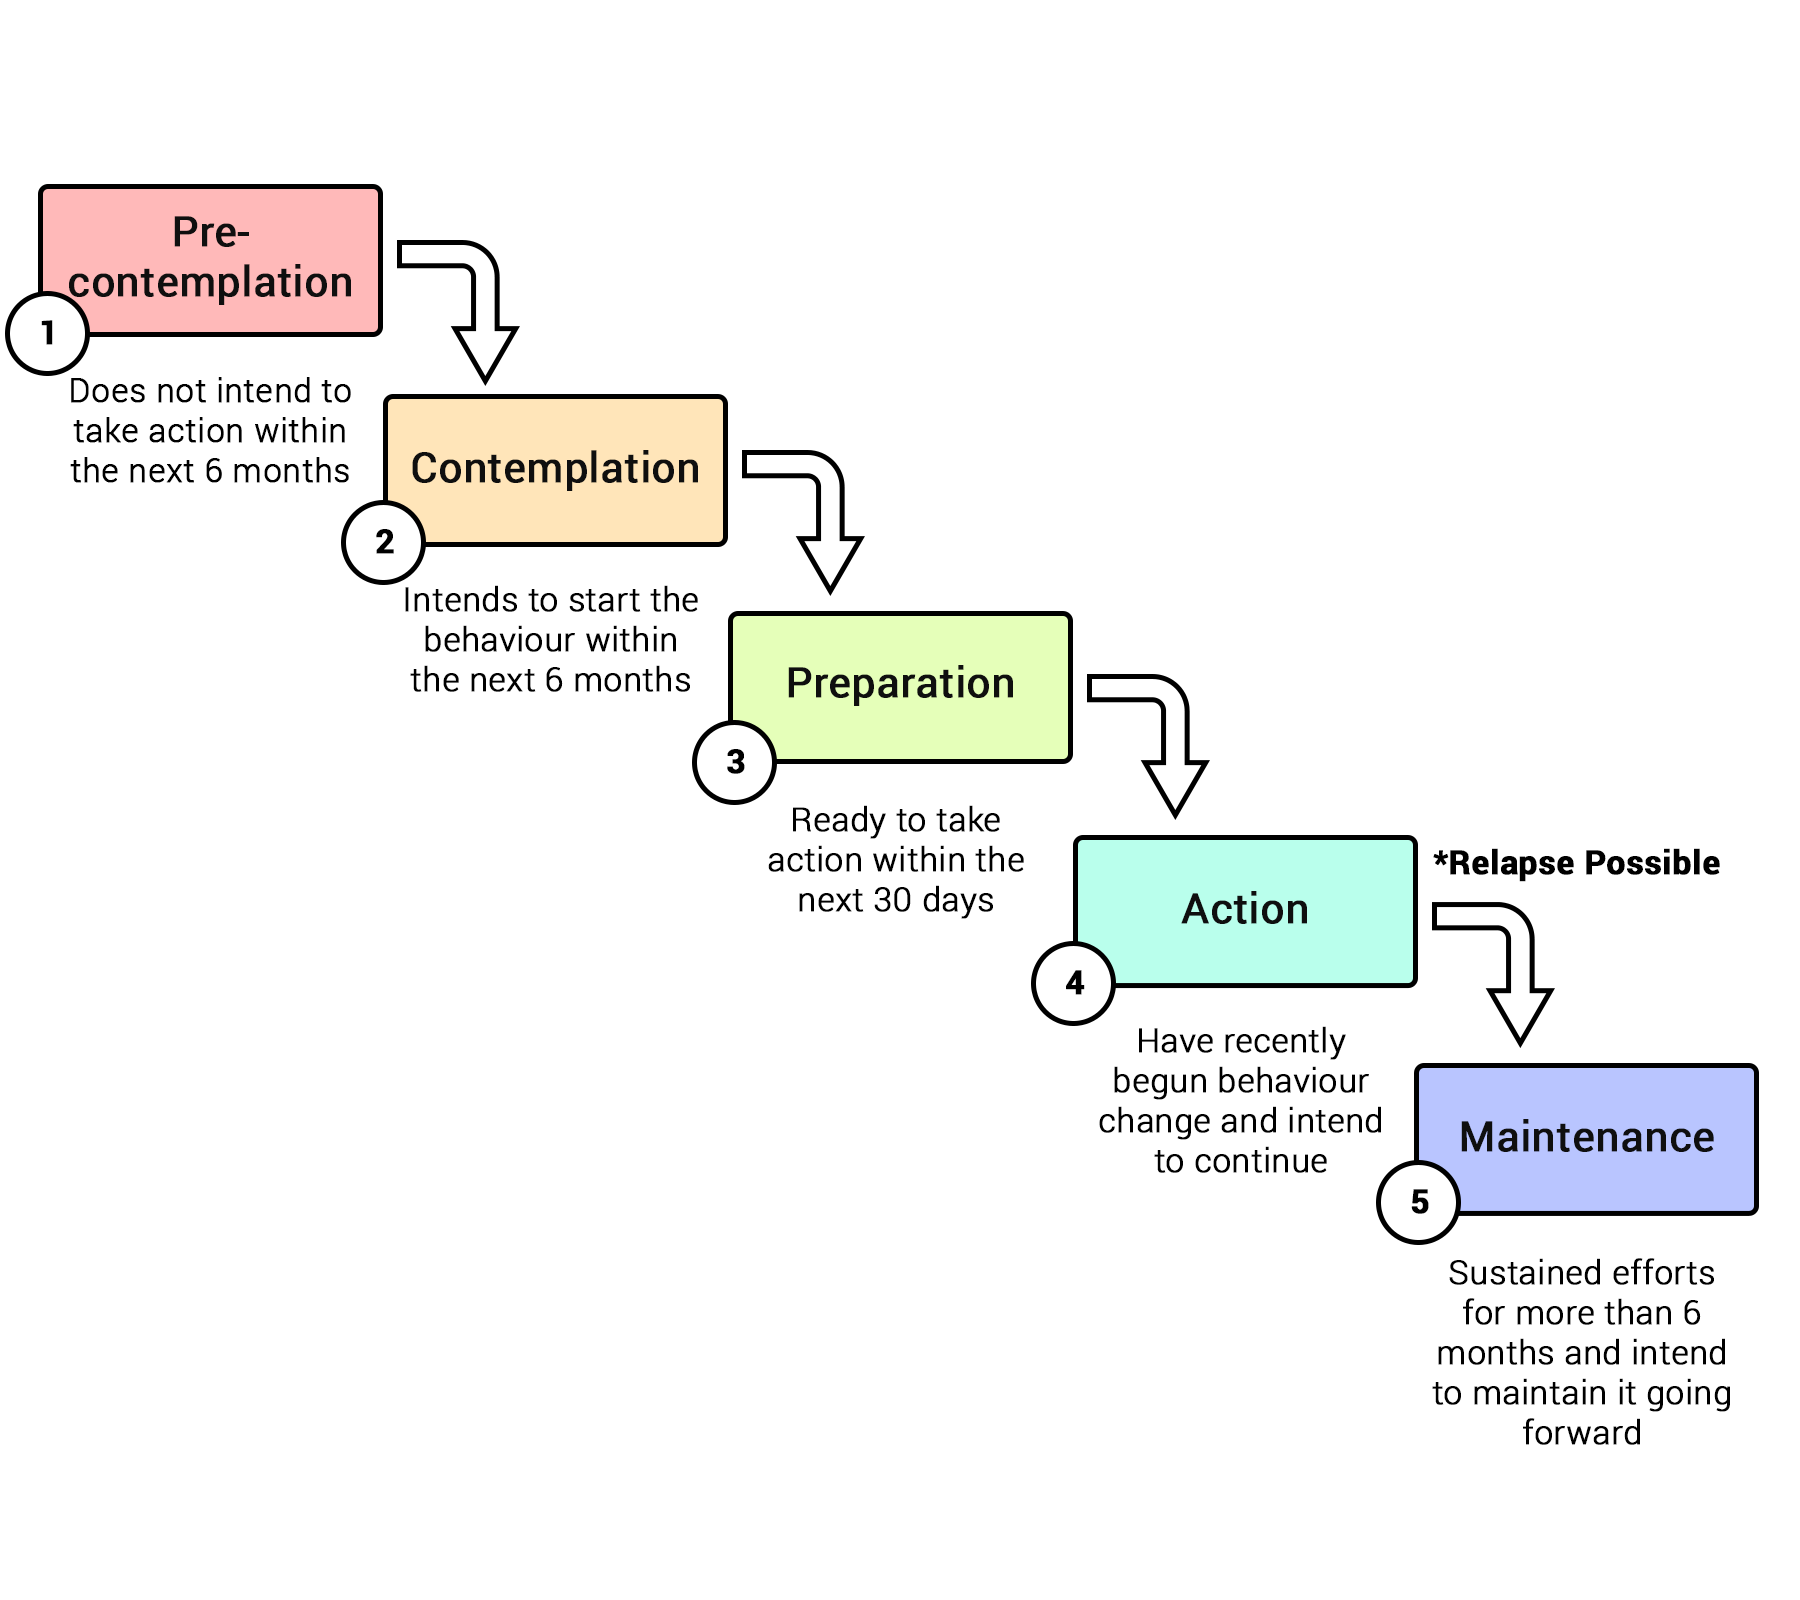
\includegraphics[scale=0.16, angle=0]{Files/prevention-study-1/figures/ttm-stages-model}
    \caption{Stages of behaviour change within the transtheoretical model.}
    \label{fig: ttm-model}
\end{figure}


The model was first developed in relation to smoking cessation, however, has since been adapted and applied to various other behaviours \cite{Nisbet2008}. The benefit of the stage model is that individuals who are at the same stage will be facing similar challenges, and therefore can be aided with the same style of intervention \cite{Morris2012a}. Each stage consists of various processes, as outlined in Table \ref{tbl: ttm-states-description}, which are carried out by the individual before they progress to the next stage.

\begin{sidewaystable}[ph!]
\centering
\caption{Stages and Processes of the Transtheoretical Model of Behaviour Change.}
\label{tbl: ttm-states-description}
\resizebox{23cm}{!}{% Resize
\begin{tabular}{llll}
\hline
Stage & Stage Definition & Process & Process Definition \\ \hline
\multirow{3}{*}{Pre-contemplation} & \multirow{3}{*}{\begin{tabular}[c]{@{}l@{}}Individual is unaware of the problem; \\ No intention to change in foreseeable future\end{tabular}} & Consciousness raising & \begin{tabular}[c]{@{}l@{}}Increasing information about \\ self and problem\end{tabular} \\
 &  & Dramatic relief & \begin{tabular}[c]{@{}l@{}}Experiencing and expressing feelings \\ about problems and situation\end{tabular} \\
 &  & Environmental re-evaluation & \begin{tabular}[c]{@{}l@{}}Assessing how one's problem \\ affects physical environment\end{tabular} \\ \hline
Contemplation & \begin{tabular}[c]{@{}l@{}}Individual is aware of the problem; \\ Serious consideration of change in behaviour\end{tabular} & Self-re-evaluation & \begin{tabular}[c]{@{}l@{}}Assessing how one feels and\\ thinks about oneself with \\ respect to a problem\end{tabular} \\ \hline
Preparation & Individual is intending to take action & Self-liberation & \begin{tabular}[c]{@{}l@{}}Choosing and commitment \\ to act or a belief in ability to change\end{tabular} \\ \hline
\multirow{4}{*}{Action} & \multirow{4}{*}{\begin{tabular}[c]{@{}l@{}}Individuals modify their behaviours, experiences \\ and/or environment in order to overcome problem\end{tabular}} & Counter-conditioning & \begin{tabular}[c]{@{}l@{}}Substituting alternatives for problem \\ behaviours\end{tabular} \\
 &  & Stimulus control & \begin{tabular}[c]{@{}l@{}}Avoiding or countering stimuli that \\ elicit problem behaviours\end{tabular} \\
 &  & Helping relationships & \begin{tabular}[c]{@{}l@{}}Being open and trusting with \\ problems to someone\end{tabular} \\
 &  & Reinforcement management & \begin{tabular}[c]{@{}l@{}}Rewarding one's self or being \\ rewarded by others\end{tabular} \\ \hline
Maintenance & Individual works to prevent relapse and consolidate gains & Social Liberation & \begin{tabular}[c]{@{}l@{}}Increasing alternatives for \\ non-problem behaviours available \\ in society\end{tabular} \\ \hline
Relapse & Individual's behaviours relapse to any previous stage & Re-engagement & \begin{tabular}[c]{@{}l@{}}Reminding one's self of previous\\  effort to change behaviour\end{tabular} \\ \hline
\end{tabular}
}
\end{sidewaystable}

\subsection{Aiding Progression via Technology Injection}
From the literature review it was identified that there are various opportunities for technology to support the necessary processes at each stage in the TTM (refer to Table \ref{tbl: ttm-states-description}, especially within the contemplation, preparation and action stages. The following sub-sections examine these concepts in further detail.

\subsubsection{Contemplation}
The contemplation state posits that the individual is aware of the problem and is serious in their consideration of changing their behaviour. The process associated with this state is \textit{Self-Re-evaluation}, which is an assessment of how one feels and thinks about oneself, with respect to the problem. The key to his process for the individual is understanding the problem and understanding their behaviour. This can be facilitated through technology by education of risk factors, presentation of current behaviours effect on risk and suggesting tools for support.

\subsubsection{Preparation}
The preparation state posits that the individual is intending to take action, typically within the next 30 days. The process associated with this state is \textit{Self-liberation}, which is when the individual commits to act or truly believes in their ability to change. At this point, technology can benefit the individual through ease of accessibility, both software and hardware based. This is especially the case for smartphone apps.

\subsubsection{Action} \label{subsubsection: ttm-action-phase}
The action state posits that the individual is now actively changing their behaviours, their experiences or the environment in order to address the problem. The action state contains numerous processes, each with their own opportunities for technology injection.

\textbf{Reinforcement management.} This process rewards the individual for their efforts and achievements, either by one's self or by others. Technology has numerous ways by which to deliver rewards, from other individuals, or from the technology itself. In the case of smartphone apps, rewards may be given as digital trophies and achievements, or by unlocking further content-material. Such techniques are referred to as gamification, and their use has been explored in recent behaviour change studies \cite{Schoech2013}.
\newline \textbf{Helping relationships.} This process requires the individual to be open and trusting with problems to someone else. Technology can aid this process by providing access to controllable social support networks, in which support and praise can be provided. These social networks would allow individuals to share their current progress, achieved milestones and provide \& receive support from others at the same stages in their behaviour change. The use of social networks in promoting healthy behaviours has shown numerous benefits, including acting as a motivator to exercise and expanding food choices \cite{Vaterlaus2015, Kamal2014}.
\newline \textbf{Counter-conditioning.} This process involves substituting alternatives for problem behaviours (e.g., Replacing high-sugar drinks with fresh fruit drinks). Technology can help educate the individual on suitable alternatives at the point of need through information access \cite{Kamal2014, Hermawati2014, Dunford2014}. Such work has been performed with those whom diet choices can have an acute effect (e.g., diabetics) \cite{Klonoff2013}, however, has not been extended for improving behavioural choices within currently healthy individuals, with the aim of observing long-term health benefits.
\newline \textbf{Stimulus control.} This process involves avoiding or countering stimuli that can elicit problem behaviours. Technology's opportunities here are somewhat limited. Ubiquitous computing researchers have envisioned scenarios in which ``just-in-time'' technologies, harnessing information about location, past-activities and user-context, can detect when a user would require assistance to motivate them to avoid negative outcomes \cite{Intille2004}. An example use-case would be the detection of fast-food outlets in the user's proximate location and the current time is lunch time, thus inferring the user is going to eat fast food. The user would then receive an alert or some form of contact from the technology advising them to avoid this action.

\subsection{Reporting Behaviours} \label{subsection-reportingbehaviours}
To accurately assess the effect of a behaviour change intervention, the validity of the behaviours reported must be accurate. There are numerous methods by which behaviours can be recorded within an intervention, including diaries, self-reporting questionnaires, direct observation and by proxy reports \cite{Elliott2014}.

\textbf{Diaries.} Diaries present a low cost, easily maintained and time efficient method of recording behaviours, however, are open to cognitive bias due to subjective self-assessment and rely heavily on the person’s ability to accurately recall past events \cite{Stone2002}.

\textbf{Direct Observation.} Direct observation offers health investigators an accurate portrayal of behaviours within the given window of observation \cite{Prince2008}. They are believed to offer more truthful recordings and can be used as a method to increase precision and accuracy for the purposes of validating self-reported behaviours. With regard to monitoring physical behaviours, total energy expenditure can be calculated using calorimetry (i.e. double labelled water), heart rate monitors and motion sensors \cite{Prince2008}. Whilst such approaches offer exceptional accuracy, they are intrusive, expensive and time intensive. It is also the case that the Hawthorne effect, commonly referred to as the observer effect, may change how an individual behaves under direct observation, and observations made may not be a true reflection of their behaviours outside of the observation window \cite{McCarney2007}.

\textbf{Self-reporting.} Self-reported questionnaires are commonly used in large-scale longitudinal studies, due to their uniformity in questioning, repeatability and ability to extract qualitative and quantitative information \cite{DiMarco2014}. Quantitative orientated questionnaires, seeking to gather quantifiable information about past-events, such as the ‘number of glasses of water consumed today’, can be at risk of cognitive bias and recall inaccuracy. Nevertheless, a comparative study seeking to validate previous day recall accuracy for active and sedentary behaviours when compared to direct observation found agreement of 85\% or higher in certain conditions, and suggests adults can accurately report their behaviours using previous day recall \cite{KozeyKeadle2014}.

\textbf{By proxy.} Proxy reporting is typically used when the subject in examination is somehow dependant on another adult, such as young children and the elderly. A study assessing the level of agreement between 6,425 children and their parents regarding dietary, physical and sedentary behaviours reported a mean agreement rate of 43\% \cite{Rebholz2014}. Similarly, studies assessing memory recall for the same events in children, young adults and the elderly showed that the reports of the elderly were as complete as the children’s, however, were the least accurate overall \cite{Gawrylowicz2014}. This highlights both the potential inaccuracies of self-reporting within certain cohorts, and the need for ground-truth data due to the rate of disagreement found in reporting utilising a proxy.
%VIVA: Chris comment - I guess it could be a discussion point duringt he viva which of these are best and why did you choose the approach that you did choose.

\subsection{Improving Reporting via Ubiquitous Computing}
Whilst a variety of approaches can be employed to record behaviours, each has their own distinctive weaknesses relating to accuracy, repeatability, scalability and cost \cite{Prince2008}. The need for an objective mediator to draw agreement across the various approaches is desired. Pervasive computing may provide such a solution.

The widespread public adoption of smartphones, smartwatches, and wearable technology, has enabled computing to become truly ubiquitous. Wireless digital devices can enable the digitisation of an individual's behaviours, often without the need for any active interaction from the user. Wearable wrist-worn devices can be used to calculate an individual’s energy expenditure and step count \cite{Pande2013}, their current activity \cite{Cleland2013}, sleep quality \cite{Noor2013}, and heart rate \cite{Parak2014}. Smartphones, via the use of on-board accelerometers and GPS, can also track physical activity levels \cite{Ozdalga2012} and sleep patterns \cite{Min2014}, whilst various apps encourage self-reporting of food consumption, enabling immediate calculation of calorie consumption \cite{Ozdalga2012}. In addition, social media websites contain a plethora of social interactions that can be analysed for behavioural trends \cite{Ruths2014}. There is an abundance of potential use-cases for such technology in the self-management of one’s health, however, the adoption of this technology for the purpose of public health education or behavioural change interventions are extremely limited. Eric Topol, a physician who has been heavily involved with wireless medicine since its inception, states in his book:
\begin{displayquote}
\textit{``Our health care approach is reactive, and, as a result, we have a world of chronic diseases, most of which are poorly managed, such as congestive heart failure, high blood pressure, and diabetes, or not managed at all, as in the case of Alzheimer’s''}
\begin{center}
	\rule{1cm}{0.4pt}
\end{center}
\textit{``Now comes a new wave of technology to not only improve the outlook for the chronic diseases of today but shift the capability, for the first time, to true prevention.''} \cite{Topol2012}.
\end{displayquote}

To leverage this opportunity, we must understand how to engage users with the new technology, and motivate them to ensure continual progression over time. Therefore, it is of paramount importance that maintaining engagement is highlighted as a key area of focus.

\subsection{Maintaining Engagement}
Evidence from internet based interventions suggest that repeated visits are necessary to achieve sustainable change \cite{Brouwer2011a}. Nevertheless, visitor engagement with these interventions is typically lower than expected, with many users opting out before becoming fully exposed to all the intervention material, resulting in suboptimal outcomes \cite{Brouwer2011a}. There is therefore the need to encourage and maintain engagement with interventions, whilst enhancing an individual’s motivations to return at a later date.

\subsection{Promoting Engagement via Technology}
Gamification is the application of game design techniques and mechanics to non-gaming domains \cite{Deterding2011}. To encourage engagement within a game, game designers utilise mechanics such as points, level-systems, avatars, badges, and leaderboards. These reward systems encourage continual progression, with the ultimate aim of maintaining engagement. Recently, there has been a surge of interest in the use of gamification for behaviour change studies, given that these reward systems help to promote engagement. Young adults and children are especially attracted to games, with virtually all young children having access to gaming consoles, computers and smartphone games \cite{Schoech2013}. As such, gamification elements have been used to educate and encourage desirable behaviours in children, such as increasing intake of fruits and vegetables through the use of fictional avatars \cite{Jones2014}, preventative education on substance-abuse and risk using smartphone and tablet apps \cite{Fiellin2014}, and an obesity prevention intervention via mobile and web platforms \cite{Delisle2015}. The use of gamification in adult behaviour change studies, however, is limited.
For health-conscious adults, commercially available smartphone apps and activity tracker companies, such as Strava, FitBit, and Nike, use gamification elements extensively in their efforts to maintain and promote continual engagement. Whilst each platform has their own approach they all record health related data, with examples including the monitoring of physical activity levels, tracking meals and monitoring sleep quality. From these data various performance metrics are calculated from which achievements are rewarded, such as badges and trophies. In addition, a user can view, typically at a high level via interactive graphs, their performances across time, allowing them to become informed of their behaviours and their resulting outcomes. Social sharing of recorded data also plays a role in enabling gamification elements, such as leaderboards, allowing users to compare their efforts with those of others. Apple and Google, whose smartphone platforms combined, account for 96.3\% of the worldwide market share \cite{InternationalDataCorporation2015}, are now shipped with iOS Health kit and Google Fit services pre-installed. The aforementioned services are proprietary to their platforms, however, act to consolidate the available data of various health-related apps and activity trackers into one common interface. The inclusion of such services into the base functionality of the most extensively adopted smartphone platforms in the world, show the market’s anticipation of widespread adoption of health-related apps.
It is therefore hypothesised that the combination of constantly accessible, highly interactive, and individually tailored feedback, combined with gamification elements, such as rewards and leaderboards, would have the largest opportunity to maintain and encourage engagement with adults in a behaviour change study \cite{Middelweerd2014}, given the advantages that each elements brings.
%VIVA: Chris - comment: This will probably be a discussion point.  Be prepared to discuss the rationale of this choice.
\section{Stakeholders and Requirements}
This Section details the development of a framework to guide the implementation of a technologically based approach to behaviour change interventions.

\subsection{The Stakeholders}
The stakeholders of any intervention consist of the End-User/Study Participant (EU), and the Health Investigator/Study-coordinator (HI)
The primary objective of the HI is to obtain accurate information on behaviours of the EU, and their effects on observable health outcomes. The HI plays a large role in the design of the intervention through the scope of their research question. As such, they strongly influence the non-functional requirements of a suitable intervention platform.

\subsection{Non-Functional Requirements}
From analysis of existing approaches of behaviour change interventions \cite{Prochaska2005,Ruiter2014}, commercial health promotion apps \cite{Ozdalga2012, Higgins2016} and software engineering best practices \cite{Fielding2000, Jones2010}, a number of non-functional requirements have been identified by the author. These requirements are not specific `features' of a system, they are the desired characteristics that influence the design of the system architecture, and are listed below:

\textbf{Accessibility.}
There should be minimal barriers/restrictions for the user to obtain the solution.

\textbf{Availability.}
The intended solution must be available to the end-user at the point of need.
\\Availability of observed data for the HI must be as close to real-time as possible.

\textbf{Extensibility.}
The solution should facilitate data exchange between other health related apps to reduce the burden of duplicating user effort to enter data.

\textbf{Privacy.}
The solution must disclose to the user where their data is stored, who can access the data and permit the user to revoke access to their data.

\textbf{Security.}
Access control must be included for all users of the solution.
\\End-Users must register to use the solution and obtain content.
\\A single user may not view another user's data.
\\Access to user data must require approved authentication from administrator.

\textbf{Scalability.}
Must be able to be used by varying numbers of users, and handle varying amounts of data.

\textbf{Tracking User Interaction.}
The solution must be capable of tracking user interactions with the system (e.g., tracking number of times a function has been used).

\textbf{Updatability.}
All content within the solution must be manageable by an administrator. This is important to keep content up-to-date as new scientific evidence becomes available.

\textbf{Usability.}
The solution must adhere to the selected platforms standards and follow best practice guidelines. This will reduce effort required to learn the solution and benefit the user through familiarity.

\textbf{Validity.}
All reported user data must be valid and testable. This includes dates, self-reported behaviours and interaction data.

\subsubsection{Platform Selection}
Consideration of the identified non-functional requirements narrows the scope of suitable platforms from which a solution can be developed. A number of key requirements directly influence the technology platform choice: Availability, Accessibility and Scalability.
Evidently, internet technologies and smartphones can address these  requirements, as they are now considered ubiquitous. As of March 2015, the smartphone surpassed the desktop in the U.S as the primary method to access the internet \cite{ComScore} (refer to Figure \ref{fig: graph-internetuse}).

\begin{figure}[h]
	\begin{tikzpicture}
	\begin{axis}[
		height=6cm,
		width=0.9\linewidth,
		%xlabel={Month},
		ylabel={\% Users},
		symbolic x coords={Mar14,Apr14,May14,Jun14,Jul14,Aug14,Sep14,Oct14,Nov14,Dec14,Jan15,Feb15,Mar15}
		]
	\addplot table [x=month, y=mobile, col sep=comma]{Files/prevention-study-1/data/internetuse.csv};\addlegendentry{Smartphone}
	\addplot table [x=month, y=desktop, col sep=comma]{Files/prevention-study-1/data/internetuse.csv};\addlegendentry{Desktop}
	\end{axis}
	\end{tikzpicture}
	\caption{Percentage share of the population who use digital devices to access the internet, for each platform.}
    \label{fig: graph-internetuse}
\end{figure}

This puts the smartphone in a unparalleled position as a suitable platform to deliver a health intervention to users. As such. for the general user, the smartphone should always be considered as the primary technology platform from which to base technological development.
There are some exceptions to this approach however, as in some cases additional analysis of technology ownership and literacy amongst the target cohort may need to be considered. For example, a technology-based intervention for seniors may require additional requirements gathering regarding the most suitable platform, given the negative correlation between age, smartphone ownership, and computing literacy \cite{Migo2015}.

\section{A Process Framework}
This Section details the recommended procedure which should be followed to implement a technology based solution for health behaviour interventions.

\subsection{Examining Relationships}
Conceptually, the entities within the framework can be modelled in an entity relationship (ER) diagram, as presented in Figure \ref{fig: erd-model}.

\begin{figure}[h]
    \centering
    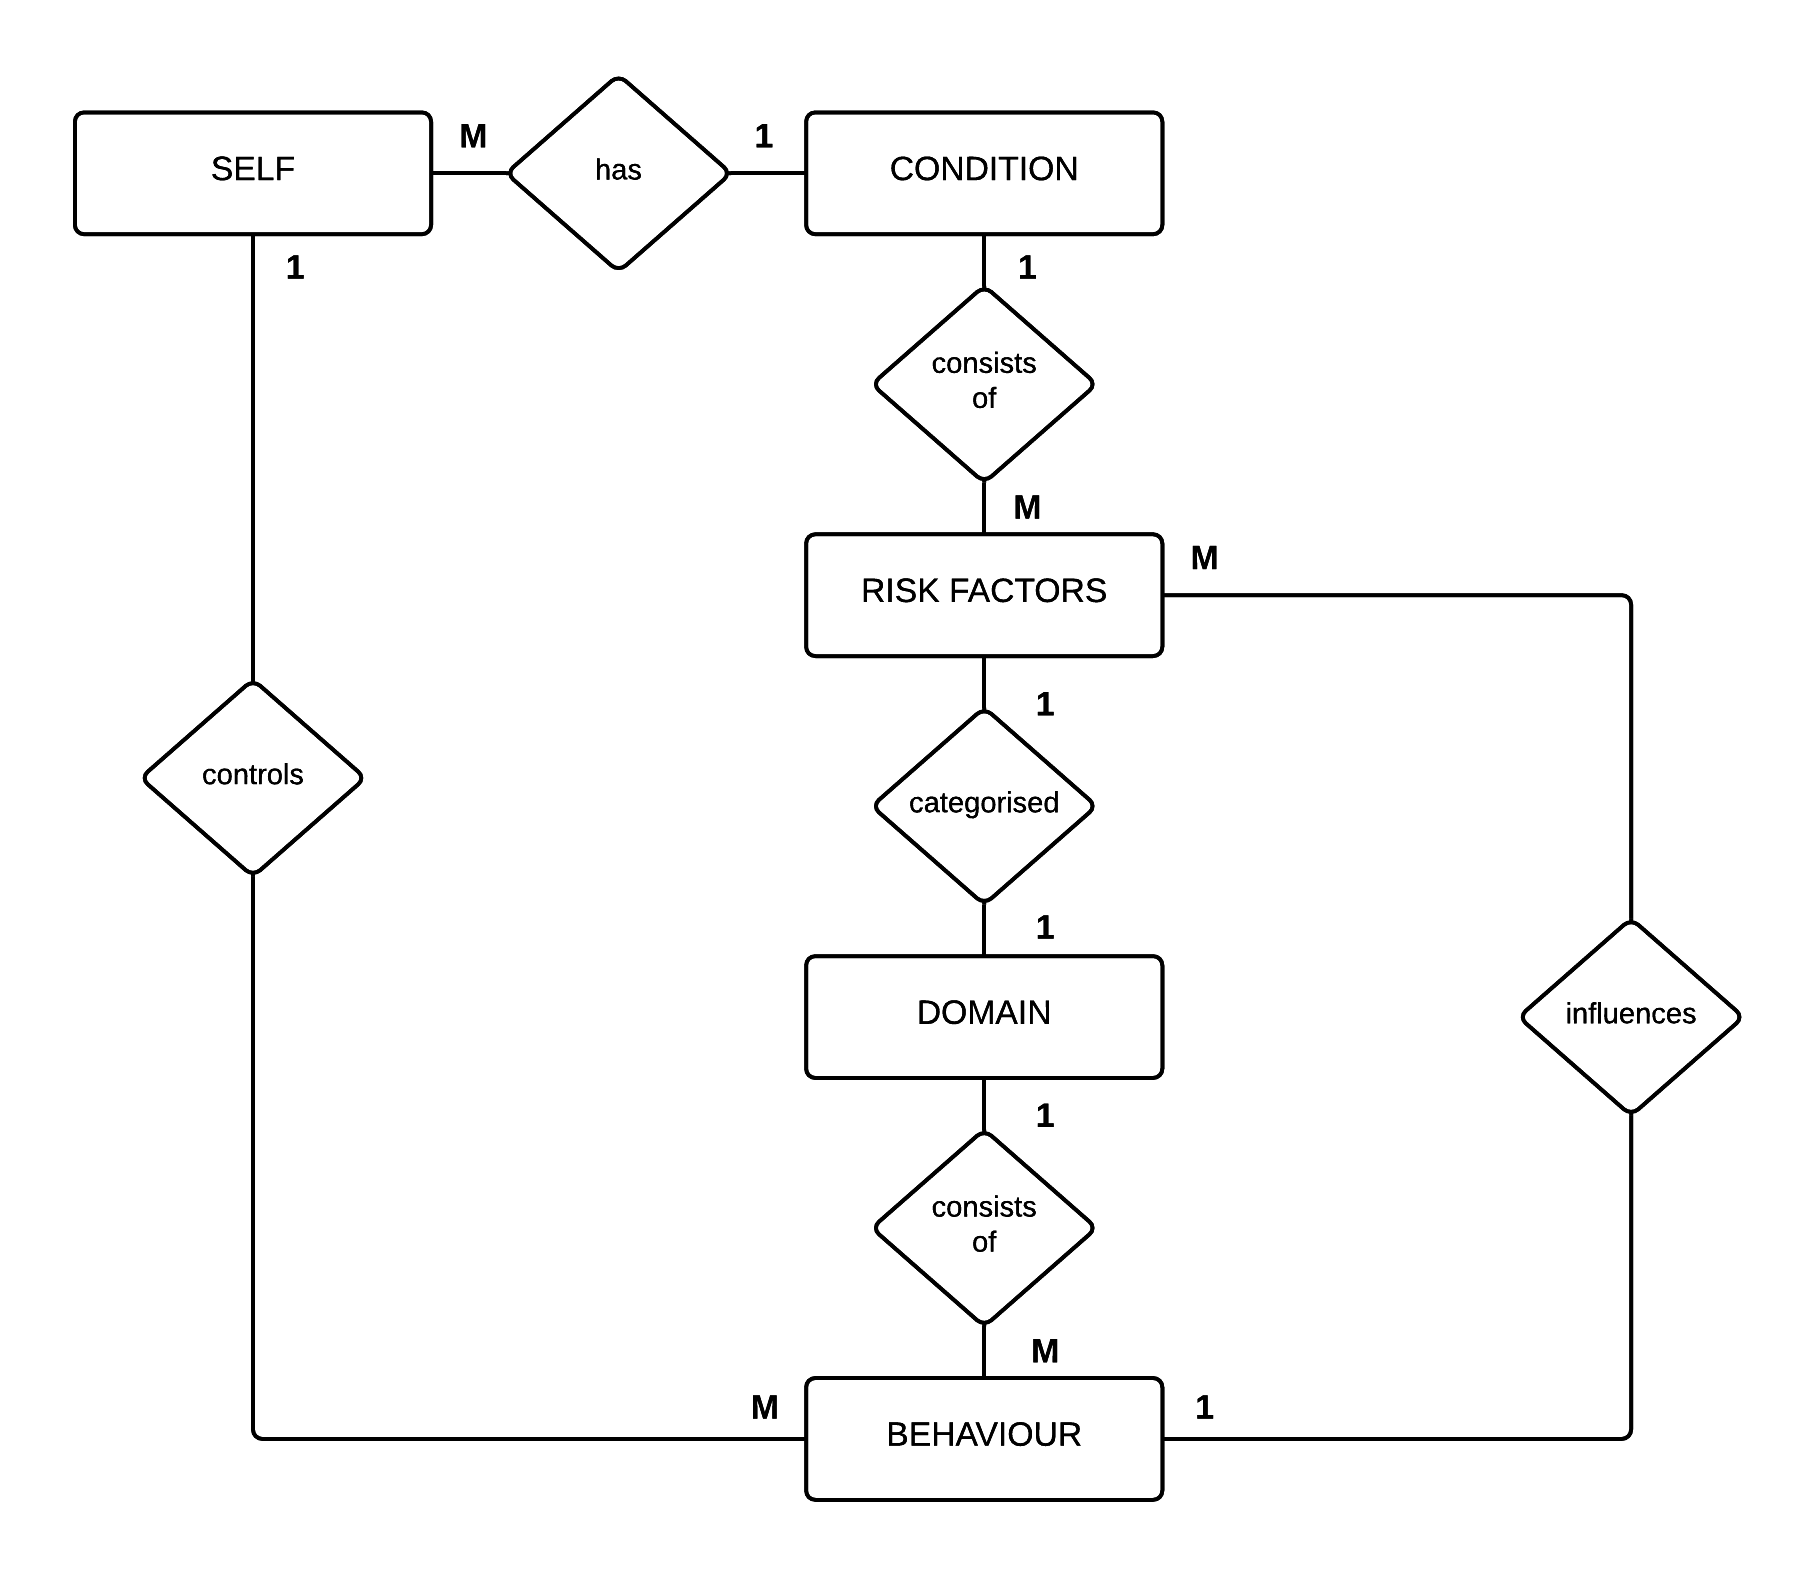
\includegraphics[scale=0.9, angle=0]{Files/prevention-study-1/figures/erd-riskfactors}
    \caption{Entity Relationship Model of Health Condition, Associated Risk Factors and Behaviours.}
    \label{fig: erd-model}
\end{figure}

The ER diagram explores the interdependencies between a person (Self), their health condition, and its' associated risk factors, and behaviours. The model posits that a condition (e.g., Heart disease) consists of multiple risk factors (e.g., hypertension, obesity), which can be categorised into various high-level domains (e.g., stress, diet). These domains have associated behaviours (e.g., working long hours, high sugar consumption), which a person has direct control over. This control can be applied to influence the numerous risk factors and ultimately alter the status of the condition, both reactively and preventatively.
Whilst each element must be understood in further detail to create a health intervention program, the author has developed process guide from which to follow.

\subsection{A Process Guide} \label{subsection: framework-process}
To guide the development of the technological intervention in the most effective manner, a procedural guide has been designed by the author. The guide details a strategy for each step of the process, based upon existing evidence and available technologies.

The steps of the process are:
\begin{enumerate}[noitemsep,topsep=0pt]
\item Establish Condition of Interest
\item Establish Modifiable Behaviours
\item Establish Key Measures
\item Create Behavioural Targets
\item Generate Health Education Literature
\item Develop Education Delivery Mechanism
\item Develop Tracking Tools
\item Create Tools for Health Investigators
\item Evaluate via Expert Assessment
\end{enumerate}

\subsubsection{Clinically Focused}
The first 5 steps of the process are clinically focused and should be performed sequentially.

\textbf{1. Establish Condition of Interest} \\
The health condition which the intervention is to be targeted must be identified. A full literature review should be performed on the condition to establish the identified etiologies and risk factors.

\textbf{2. Establish Modifiable Behaviours} \\
Once all risk factors are established, each should be examined to establish those which are non-genetic, or modifiable. Modifiable risk factors are not limited to human behaviour, however, may also be related to the environment. Various environmental factors can be altered through behaviour change, and so should be considered \cite{Kujala2002}.

\textbf{3. Establish Key Measures}\\
For each modifiable risk factor, establish the standard methods of assessment. The format of these measurements are expected to be vary, however, by default will include physiological and behavioural measures.
\begin{itemize}[noitemsep,topsep=0pt]
\item \emph{Physiological} measures include quantitative measurement of the human structure, anthropometric assessments, uranalysis, and blood specimen analysis \cite{Oberg2014}.
\item \emph{Behavioural} measures include an array of behavioural assessments; including readiness-for-change, sleep quality, social engagement, depression, and couple satisfaction questionnaires  \cite{Martin2007}.
\end{itemize}

Additional measurements can be included on a case-by-case basis, depending upon the condition. For example, an intervention for a respiratory conditions may wish to use lung function tests, such as spirometry, whilst a focus on cognitive impairment may wish to use a battery of neurological examinations and brain imaging.

\textbf{4. Create Behavioural Targets} \\
Using the information established in steps 2 and 3, it is possible to set targets for desirable behaviours to mitigate the risk factors. Behavioural goals based upon scientific evidence may already exist, and have been established by governments or health officials. Firstly, examine these existing recommendations. If more than one recommendation exists, use that which has the greatest scientific grounding for the targeted condition or age-group \cite{Stover2002, Pronk2004}.

\textbf{5. Generate Health Education Literature} \\
It may be necessary to repurpose the scientific literature identified in the previous steps into layman's terms\footnote{Using words and terms that the average individual, or someone without professional training in the subject area, can understand.}, depending upon its complexity.
There are a few general principles relating to education \cite{Gilbert2010} that should be considered:
\begin{itemize}[noitemsep,topsep=0pt]
\item To facilitate learning, repetition is generally required.
\item Recent experiences are more vivid than past.
\item Behaviours or skills must be practiced.
\item Learning is more effective when the learner is motivated by results.
\item The higher the education level, the greater the effectiveness of written word.
\item The lower the education level, the greater the need for visual or oral media.
\end{itemize}

%VIVA: Chris - comment about Fact Bank - Has anyone else tried this approach?
Considering these principles, it is advised that a fact bank is created, containing short and impactful facts about the health condition. To supplement each fact, an example of a related behaviour and a positive health outcome should be attached. These should be presented to the user as often as possible to increase exposure and support learning. An example:
\begin{displayquote}
\textit{``Diabetes is the leading cause of blindness in working-age adults''}
\begin{center}
	\rule{1cm}{0.4pt}
\end{center}
\textit{``Exercise is one of the most important things you can do to take control over diabetes. The key is to find something you enjoy doing and stick with it. It can be walking, swimming, cycling, or dancing — just get moving!. Aim for 30 minutes of activity, five days per week.''}
\end{displayquote}

This format follows the principles of education, and presents a fact about the condition which motivates the person to act based upon desirable results. This is then reinforced through suggestions of actions to achieve the desired result. This particular example may be accompanied with visual cues related to blindness and exercise.

\subsubsection{Software Focused}
The initial clinically focused steps are not innovative from a clinical or public health perspective, however, their inclusion in the guide seeks to educate those from other domains, e.g., computer science, of the necessary precursory steps that should occur before technology is injected. The latter stages are predominately software focused, nonetheless, they rely heavily upon on the quality and validity of the findings in the clinical stages. The software focused stages can be performed concurrently and should be approached following an agile methodology.

\textbf{5. Develop Education Delivery Mechanism}\\
Using the health education literature, a suitable mechanism should be developed to present this information to the user. A mechanism unique to smartphones, and smartwatches, are notifications. These can be configured to be delivered at set times, or at particular contexts, inferred from sensors. Their representation may include badges, sounds or a custom text alert.
The use of sound in notifications in smartphones is recommended to prompt the user to act upon them \cite{AppleNotifications2015} even if the user is not using the device. For the purpose of delivering the health education information in a notification, the amount of text should be limited. Having considered the principles outlined in Step 5, the fact portion is an ideal amount of text to display in the message body. Upon interaction with this text, the user may be presented with the additional lifestyle suggestion.
%VIVA: How limited should the notification be? Are there any platform restrains? Character counts etc?

\textbf{6. Develop Tracking Tools} \\
To aid the progression of behaviour change, tools should be developed which allow the study participant to quantify their behaviours in the relevant domains. The tools may be a user interface, that allow for manual self-reporting of behaviours, or they may use existing data sources to extract relevant behaviours.

\textit{Goal Setting.} Primarily, the tools should encourage users to achieve the recommended targets identified in Step 4. These targets can be considered global targets, however, many individuals may require a tailored step-wise progression to reach these targets \cite{Prochaska2013}. Often when faced with targets that are deemed as unattainable, or too difficult, relapse occurs \cite{Velicer1995, Prochaska2005}. As such it is important to allow the personalisation of goals. These goals may be configured to within each individual's capabilities upon commencement of the intervention. For example, for a morbidly obese person, it may not be possible to achieve the recommended target of 30 minutes of physical activity (running), five times per week. It is, however, possible to achieve 3 minutes, 3 times per week, and so this should be the personalised goal. As the individual becomes competent in achieving these levels of activity, new goals are set, until eventually the personal goal meets or exceeds the global targets identified in Step 4.
From the health investigators perspective it is is possible to measure individual progress using these personalised goals, whilst using global recommendations allows a standardised way to measure progress across the entire cohort.

\textit{User Interactions.} In addition to behavioural data, user interactions and usage patterns should be observed for the benefit of the application designers and health investigators. The data generated can provide investigators with an insight into how the app is actually being used. At a high level, it is possible to see the number of times a function was used, or the time spent on a particular screen, or what time of day the app was launched. Further examination of interaction data can also highlight if features fulfil their intended purpose, whilst also identifying problematic areas of the app, flagging them to be addressed in future updates.
%VIVA: Chris comment RE: Future updates. I think this is an important point,  however,  at times I feel we record all of the data and then do not properly analyse it or have the ability to actually understand what it means without a gold standard.  This could make for an interesting discussion point.

\textit{Uploading Frequency.} The uploading of participant data should be as close to real-time as is possible for 2 reasons:
\begin{enumerate}[noitemsep,topsep=0pt]
\item To allow for accurate analysis of the data at various stages within the intervention and observe for trends or significant changes, which may be due to internal or external components of the intervention.
\item To minimise the risk of data loss if the smartphone is lost or damaged.
\end{enumerate}

\textbf{7. Develop Tools for Health Investigators} \\
Predefining and structuring a suitable data model for the intervention data will dramatically reduce the need for human pre-processing or data cleansing\footnote{the process of detecting, correcting, and/or removing corrupt and inaccurate records from a database.} in the latter stages of the intervention. A referencing system using unique keys for each participant can establish integrity between various sources, reducing the technical complexity of automated analysis.
This automated analysis may be used to observe for individual trends, monitor behaviour trajectories or detect abnormal changes within the data \cite{Hartin2015-ICOST}.
Ethical considerations of the health condition also influence the design of automated tools. If a study seeks to address depression, and the user reports suicidal tendencies via the data, it is the ethical responsibility of the HI to intervene. Rather than waiting for human detection the data entry, automatic flagging tools should be developed so that response may be swift. This, again, is another huge benefit of using technology to facilitate the entry and storage of data.

\textbf{8. Evaluate via Expert Assessment}\\
Having developed a solution, it should be peer-reviewed by experts in the domain. There are a number of methods by which a clinical intervention can be evaluated, including systematic reviews and critical appraisals \cite{Sackett1997, Morrison1999}.
To evaluate the mobile based technology solution, however, options are very limited. \citeauthor{Stoyanov2015} developed the Mobile App Rating Scale (MARS), which is a peer-reviewed, objective, multidimensional measure for trialling, classifying, and rating the quality of mobile health apps \cite{Stoyanov2015}. The scale assesses app quality across 5 core criteria: engagement, functionality, aesthetics, information quality, and subjective quality \cite{Stoyanov2015}. Within each criteria, there are a number of sub-items from which to rate (n=23). Each item is graded on a 5 point scale (1-Inadequate,\ldots, 5-Excellent).
The users who rate the developed solution using MARS should be experts within the targeted health domain. It is also recommended that they complete a training exercise before use, to develop an understanding of the scale and how to calibrate their scoring.

\section{Applying the Framework}
%VIVA: Can you defend the question if asked did you retro fit this process around what you actually produced during your research
This Section details the application of the outlined process framework to guide the design and development of the \textit{Gray Matters} smartphone app \cite{Hartin2014-IWAAL}. The Gray Matters app was used to facilitate a behaviour change intervention for middle-aged adults in a 6-month randomised control trial pilot study \cite{Norton2015-TRCI}. This Section will include details of the application area, the identification of risk factors, mapping risk factors to targets and the technical development of the solution.

\subsection{Application Area}
AD affects an estimated 44.4 Million people worldwide with a new case developing every 68 seconds. At this rate, it is predicted that by 2050, 135.5 million people will have the disease, and a new case will develop every 33 seconds \cite{Thies2013}. The financial and emotional costs of the AD have been well documented in both the public media and in the scientific literature \cite{Alz2010, Hurd2013}. Public understanding of the disease and its etiology has much room for improvement. A recent study of 1641 adults from the U.S found that as many as 39\% of respondents did not know that medications to prevent the disease were not available \cite{Roberts2014}. Typically, many attribute genetics to the development of the disease, citing that it ``runs in their family'' \cite{Lock2006, Roberts2014}. Nevertheless, all genetic factors discovered to date that are associated with AD account for approximately one third of the risk of developing the disease, leaving the majority of risk due to lifestyle and environmental factors and their effects on genetic function \cite{Ridge2013}. Importantly, such factors are modifiable and therefore have the potential to be useful targets for the prevention of cognitive decline and AD through behavioural change interventions.

\subsection{Acquiring Behavioural Targets for intervention} \label{section-acquiring-targets}
To enable an effective multi-domain intervention, targeting numerous risk factors simultaneously, a review of existing literature on AD risk was performed. Over 130 peer reviewed journals and papers were analysed, highlighting the top behaviours in which to focus future effort. These behaviours exhibited trends, which were categorised into 7 core domains: Physical, Diet, Cognitive, Sleep, Stress, Social and Smoking. The research performed is in agreement with the findings of a systematic review and Delphi consensus study into the identification of target risk factors for an AD prevention effort \cite{Deckers2015}.

\begin{table}[h]
\centering
\caption{Behavioural domains and AD related risk factors.}
\label{tbl: behavioural domains}
\resizebox{\textwidth}{!}{ %Resizes the box to fit all text
\begin{tabular}{l l c}
\toprule
Domain    & Associated Risk Factors & Key References \\ 	\midrule
Physical  & Obesity, Hypertension, Depression    & \cite{Hamer2009,Angevaren2010,Gelber2012,Buchman2012,Alonso2009,Dahl2010} \\
Diet      & Obesity, High-cholesterol, Diabetes & \cite{Lu2009,Dahl2010,Alonso2009,Creavin2012,Gaussoin2012,Gu2010,Gu2010a,Shatenstein2012} \\
Cognitive & Lack of novel or stimulating cognitive tasks & \cite{Anstey2013a,Marquie2010,Wilson2012,Valenzuela2011,Unverzagt2012} \\
Sleep     & Sleep deprivation, Amyloid-beta peptide levels & \cite{Scullin2015,DiMeco2014,Rothman2013,Musiek2015} \\
Stress	  & Depression, Hypertension, Sleep deprivation	 & \cite{Diniz2013,Boyle2010,Dotson2010,Royall2012,Potvin2011} \\
Social    & Small social network, Living alone & \cite{Frati2011, Saczynski2006, Amieva2010} \\
Smoking	  & Cerebrovascular / Coronary heart disease  & \cite{Gaussoin2012,Gelber2012,Barnes2011,Durazzo2014,Rusanen2011} \\	\bottomrule

\end{tabular}
}
\end{table}

Table \ref{tbl: behavioural domains} highlights that risk factors are unlikely to occur in isolation, can span multiple domains and are expected to interact in a synergistic or antagonistic manner. As such, the need for a multi-domain intervention, spanning all domains simultaneously, is reinforced.

The following sub-sections detail the identified domains, including further details of the risk factors and their supporting evidence. In addition, the key measures about each domain's behaviours are identified and summarised.

\subsubsection{Physical}
Physical activity's main protective effects against AD risk result from its counteracting influence on vascular risk factors such as hypertension, obesity, and diabetes \cite{Hughes2010,Angevaren2010}.
In addition to these vascular effects, physical activity has been shown to directly and independently affect the brain in animal studies \cite{Voss2013}.

Definition of the optimal dose of physical activity is difficult, because studies rarely include measures of frequency, duration or intensity of exercise. There is a growing consensus that \textit{intensity} may be the most important factor for physical adaptation and cardiovascular disease prevention \cite{Kaminsky2014,Wilson2015,Weston2014}. In an effort to improve public health the CDC translated scientific evidence relating to the duration and intensity of physical activity into guidelines \cite{CDC_translating}. As part of this effort, various physical activities were categorised as \textit{Moderate} and \textit{Vigorous} intensity exercises. Moderate intensity exercises include walking at a brisk pace (3 - 4.5 mph), cycling (5 - 9 mph) and gymnastics. Vigorous intensity exercises include running, cycling(\textgreater 10mph), calisthenics and jumping rope. A complete list of activities can be found in \cite{cdcpaguidelines2008}.
Adherence, however, to these recommended guidelines are low. In the United Kingdom only 35\% of men and 24\% of women achieve the recommended targets for moderate-intensity activity \cite{Miles2007}.

\subsubsection{Diet}
Extensive research has been performed on the effects of diet modification and health outcomes. In the literature of AD, the Mediterranean diet has been promoted for many years, and it is believed that adherence may protect against dementias \cite{Trichopoulou2014, Psaltopoulou2013}. A visual representation of these guidelines is presented in Figure \ref{fig: med-diet-pyramid}. The diet is characterised by:
\begin{itemize}
\item A \textbf{high} consumption of healthy oils, including fish and olive oil, nuts, vegetables, fruits, seeds and beans.
\item A \textbf{moderate} consumption of dairy products, including yoghurts and cheeses.
\item A \textbf{low} consumption of meat \cite{Gu2010a}.
\end{itemize}

\begin{figure}[h]
    \centering
    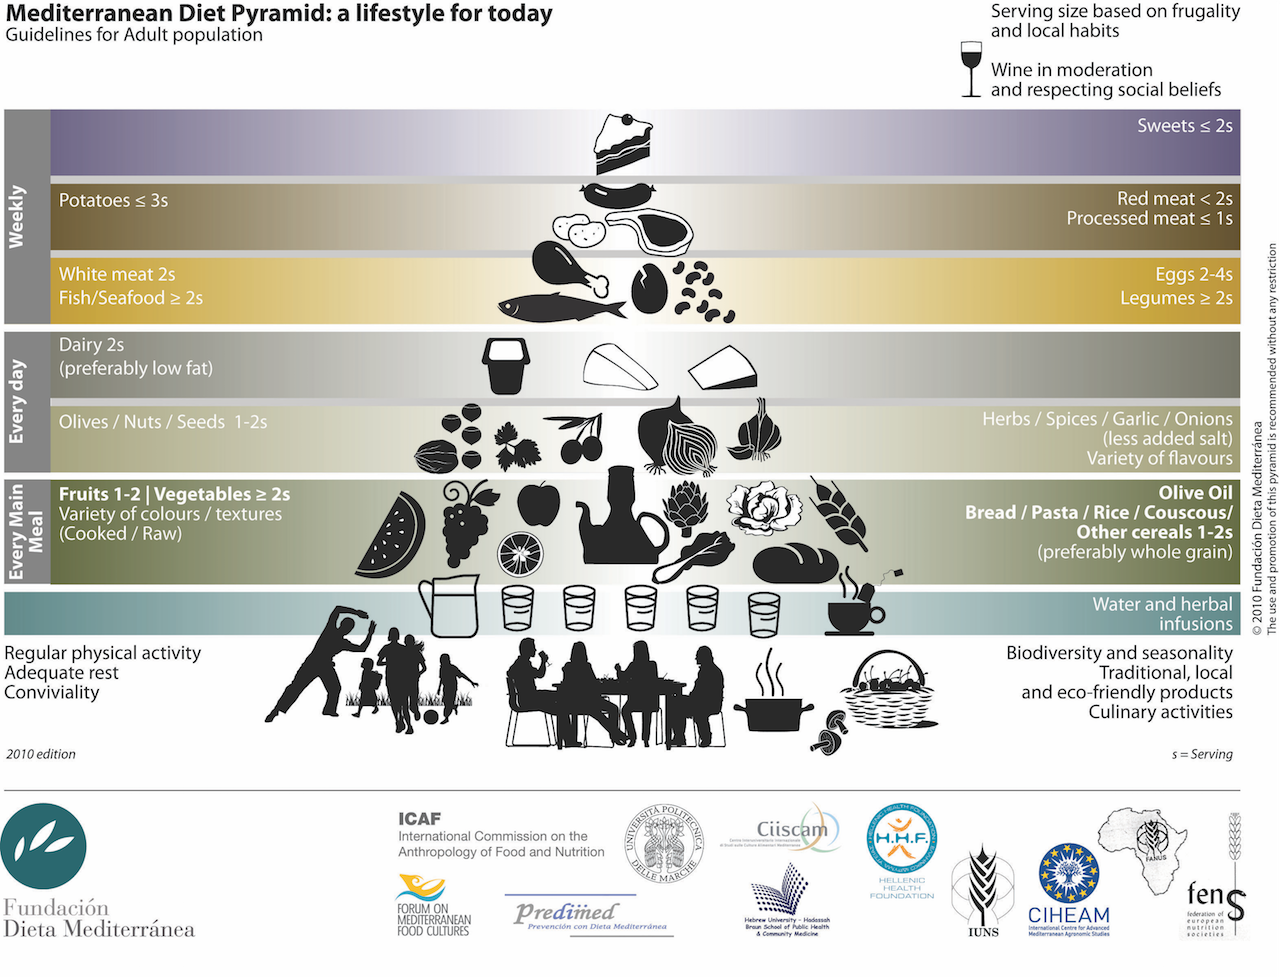
\includegraphics[scale=0.3, angle=0]{Files/prevention-study-1/figures/med-diet-pyramid-small}
    \caption{The Mediterranean Diet Pyramid.}
    \medskip
	\small
	As recommended by \cite{Bach-Faig2011}, who encourage use of this image without restriction.
    \label{fig: med-diet-pyramid}
\end{figure}

\textbf{Obesity.}
Within the body of literature relating to AD risk, it is apparent that obesity is interrelated with various other risk factors, including hypertension, diabetes, hyperlipidaemia and high-cholesterol \cite{Gustafson2012, Gustafson2008}. The role of excess adipose tissue and cognitive decline is not fully understood, however it is presumed to influence brain health via varied biological mechanisms \cite{Gustafson2012}.

\textbf{Fat Intake.}
During the literature review it was found that experts did not name fat intake as a specific risk factor \cite{Deckers2015}. Consumption of unsaturated fats, including omega-3 fatty acids which are found in nuts and fish, have been associated with a reduced risk of dementias \cite{Sydenham2012,Huhn2015} and is in accordance with the recommendations of the Mediterranean diet.

\subsubsection{Cognitive}
It is perhaps instinctual that the brain, like any other body-part, should be exercised in order to remain healthy and agile. As such, it is believed that exposure to cognitively stimulating or novel activities, such as those found in a complex work environment may protect against cognitive decline \cite{Roberts2014}. Studies on the subject have shown that high childhood school performance is protective of dementia risk, especially if the person continues to work in a complex work environment in adulthood \cite{Dekhtyar2015}. Therefore, it is now believed that increased cognitive activity during premorbid life may delay cognitive decline by increasing an individual’s cognitive reserves \cite{Sattler2012, Dekhtyar2015}.

Commercial entities have promoted the use of brain training games and apps to build a cognitive reserve \cite{Worland}. The scientific evidence on such activities is sparse and according to the editor of \textit{Cerebrum - the Dana Forum on Brain Science}:
\begin{displayquote}
``Few topics in the world of neuroscience evoke as much debate as the effectiveness of cognitive training" \cite{Boot2014}.
\end{displayquote}
The ACTIVE (Advanced Cognitive Training for Independent and Vital Elderly) trial found that cognitive training had no effect on dementia \textit{risk} after a 5 year followup \cite{Unverzagt2012}. Upon further review at 10-years, however, a follow up study reported that those who received the cognitive training showed less decline in self-reported IADL compared with the control group \cite{Rebok2014}. In addition, the study also concluded that reasoning and speed training resulted in improved targeted cognitive abilities for 10 years over control \cite{Rebok2014}.
As such, the experts in a systematic review of evidence by \citeauthor{Deckers2015} ranked cognitive activity as the 3\textsuperscript{rd} most important risk factor in their Delphi rounds. Similarly, \cite{Bavelier2013} called for a collaboration between these commercial entities and the next generation of neuroscientists, to truly leverage the opportunities provided by technology.

\subsubsection{Sleep}
There have been many studies on sleep and health outcomes. In the area of dementia, there have been a number of observational studies, using objective sleep measures (e.g., polysomonography and wrist actigraphy) and self-reporting, that support links between disturbed sleep and cognitive decline \cite{Spira2014}. An observational study of 18,631 twins found a relationship between poor sleep and life dissatisfaction, leading to increased risk of stress and depression \cite{Paunio2009}. These compounding factors are discussed further in Section \ref{target-stress}. This accumulation of poor sleep also leads to day-time sleepiness, which in a 3-year longitudinal study with 1041 participants was found to be a statistically significant independent risk factor for dementia in older adults \cite{Tsapanou2015}.
From the literature it appears that healthy sleep plays an important role in maintaining brain health in ageing \cite{Spira2014}, and an effort to improve sleep quality by minimising disturbances could potentially play a key role in dementia prevention.

\subsubsection{Stress} \label{target-stress}
The effects of stress include hypertension, depression and disturbed sleep \cite{Schneiderman2005}. Each of these have a documented relationship with AD risk. It is known that depression plays a role on executive functioning and is associated with the onset of dementias in later life \cite{Dotson2010,Royall2012,Boyle2010}. Hypertension is present in all major causes of cognitive impairment \cite{Iadecola2014}. The relationship is not fully understood, however, potential mechanisms include focal brain atrophy, ischemia, white matter disease and Amyloid accumulation \cite{Iadecola2014}. Many placebo-controlled trials aiming to lower blood pressure have been performed, which have shown positive and desirable effects \cite{Staessen2011}. These trials were performed with subjects in later life, and the results were inconclusive as to whether lowering blood pressure can \textit{reverse} AD risk.

\subsubsection{Social}
Greater levels of social engagement and participation are associated with lower rates of dementia \cite{Saczynski2006, Fratiglioni2000}. An analysis of 2089 subjects, followed over 15 years showed that it is the quality of these social relationships that is the most important factor \cite{Amieva2010}. As relationship satisfaction and reciprocity increased, dementia incidence decreased \cite{Amieva2010}. These findings may be explained due to increased cognitive stimulation, and a reduced risk of depression \cite{Saczynski2010}.

\subsubsection{Smoking}
Smoking comes with a plethora of health risks, including an increased risk of dementias \cite{cdc_smoking}. \citeauthor{Deckers2015} noted 13 studies on smoking and dementia risk, of which 10 found increased risk \cite{Deckers2015}. Experts rated smoking as the 8\textsuperscript{th} most important factor regarding AD risk as part of their Delphi analysis of existing evidence. Further analysis of these studies showed that current smokers have a 59\% increased risk of developing AD \cite{Peters2008}. As with many neurological conditions, the exact mechanisms behind the association are still unknown.

\subsubsection{Summary of Key Measures}
It is possible to quantify behaviour in each domain by monitoring key measures. Table \ref{tbl: key-measures} describes the key measures which were developed from the literature review. Many domains have more than one key measure, as many are multifaceted and complex. Note that the social domain only has one measure, which is a subjective rating of social engagement and does not measure an objective measure, such as time spent in social scenarios. This is due to the finding that quality of social relationships and interactions are the most important factor \cite{Amieva2010}.

\begin{table}[h]
\centering
\caption{Key Behaviour Measures for AD.}
\label{tbl: key-measures}
\resizebox{\textwidth}{!}{ %Resizes the box to fit all text
\begin{tabular}{@{}llll@{}}
\toprule
Domain                     & Measure                               & Unit         & Type       \\ \midrule
\multirow{2}{*}{Cognitive} & Time spent on New/Novel activities         & minutes      & objective  \\
                           & Time spent on Stimulating activities         & minutes      & objective  \\ \midrule
\multirow{3}{*}{Diet}      & Consumption of  fruits and vegetables       & cups         & objective  \\
                           & Consumption of whole grains                 & ounces       & objective  \\
                           & Consumption of nuts, seeds, or legumes      & servings     & objective  \\ \midrule
\multirow{2}{*}{Physical}  & Time spent doing moderate physical activity & minutes      & objective  \\
                           & Time spent doing vigorous physical activity & minutes      & objective  \\ \midrule
\multirow{3}{*}{Sleep}     & Rate effort to promote sleep                & rating-scale & subjective \\
                           & Self-rate sleep quality                     & rating-scale & subjective \\
                           & Duration of sleep                           & hours        & objective  \\ \midrule
Social                     & Rate social engagement                      & rating-scale & subjective \\ \midrule
\multirow{2}{*}{Stress}    & Self-rate stress level                      & rating-scale & subjective \\
                           & Effort to decrease stress                   & rating-scale & subjective \\ \bottomrule
\end{tabular}
}%end of resize
\end{table}

\subsection{Development of Delivery Mechanism and Tracking Tools}
Adopting a modular approach to the design and development of the platform enables components of the system to be added, removed or re-used in other similar systems. Given that the preparation, action and maintenance phases of the TTM consist of numerous processes, it is appropriate that a platform intending to supplement behaviour change can address each of these processes in a modular fashion. For the purpose of reducing AD risk, the components presented in Table \ref{tbl: key-measures} were therefore identified as being necessary:
\begin{itemize}
\item \textbf{Education} about AD risk and prevention strategies.
\item \textbf{Monitoring} relevant behaviours through observation or self-reporting.
\item \textbf{Feedback} provision based on observed behaviours and targets.
\end{itemize}

Using a tab-based user interface (UI) each identified component is displayed to the user as a separate tab, helping separate their functions and reducing the overlap of content and behaviour change strategies.

\subsection{AD Education Component}
To assist users in their traversal of the TTM, education plays a key role to support motivations and efficacy in achieving set goals. As the identified platform is mobile, the intended users are in need of a method to receive information in a succinct and efficient manner.

\subsubsection{Daily Facts}
For each of the core domains and associated risk factors identified in Table \ref{tbl: behavioural domains},  numerous prevention methods were identified from medical literature, and further developed by a team of psychologists, epidemiologists and nutritionists at Utah State University \cite{Norton2015-TRCI}. These risk factors and their associated prevention methods were translated into layman's terms. Each identified risk factor or behaviour was assigned one or more suggestions, thereby creating over 160 fact and suggestion pairs. These pairs are hereafter referred to as daily facts. The quantity of the daily facts are reflective of the supporting medical literature and are summarised in Table \ref{tbl: daily fact count}. An example daily fact and related suggestion from the diet domain is as follows: \textit{“Consuming high amounts of processed foods is related to cognitive decline\ldots Try a fresh salad for dinner instead of something from a box”}.
\begin{table}
\centering
\caption{Number of daily facts for each behavioural domain.}
\label{tbl: daily fact count}
\begin{tabular}{@{}l c@{}}
\toprule
Domain    & Number of Daily Fact Pairs \\ 	\midrule
Physical  & 23                              \\
Diet      & 66                              \\
Sleep     & 14                              \\
Cognitive & 24                              \\
Stress    & 10                             	\\
Social    & 27                              \\ \hline \hline
Total	  & 164								\\	\bottomrule
\end{tabular}
\end{table}

\subsubsection{Presentation of daily facts}
Information presented visually on a screen is processed differently than verbally from a person \cite{Sundar2015}. Avatars have been used extensively to facilitate the mediation of information in computer-user interactions. Their use includes user-to-user communications, social media, advertising, news-reports and job interviews \cite{Sundar2015}. The avatar acts as a visual representation of the knowledge source \cite{Bente2008} and are hypothesised to enhance social interactions \cite{Blascovich2002}. Therefore, they are also expected to increase trust in communications. Additionally, the use of certain visual characteristics of an avatar can have an effect on the rational choice that the user has on the information presented. These choices include assessing the level of uncertainty in the information  source \cite{Afifi2000}. As such, for this particular use-case a number of personas were considered to represent the knowledge source of the daily facts \cite{Sundar2015}, to best increase trust in the information presented. These included a doctor, a nurse and a coach. Relying on expert advice from psychologists at Utah State University, the coach was identified as the suitable avatar, the implementation of which is presented in Figure \ref{fig: screenshot-dailyfact}.

\begin{figure}[h]
    \centering
    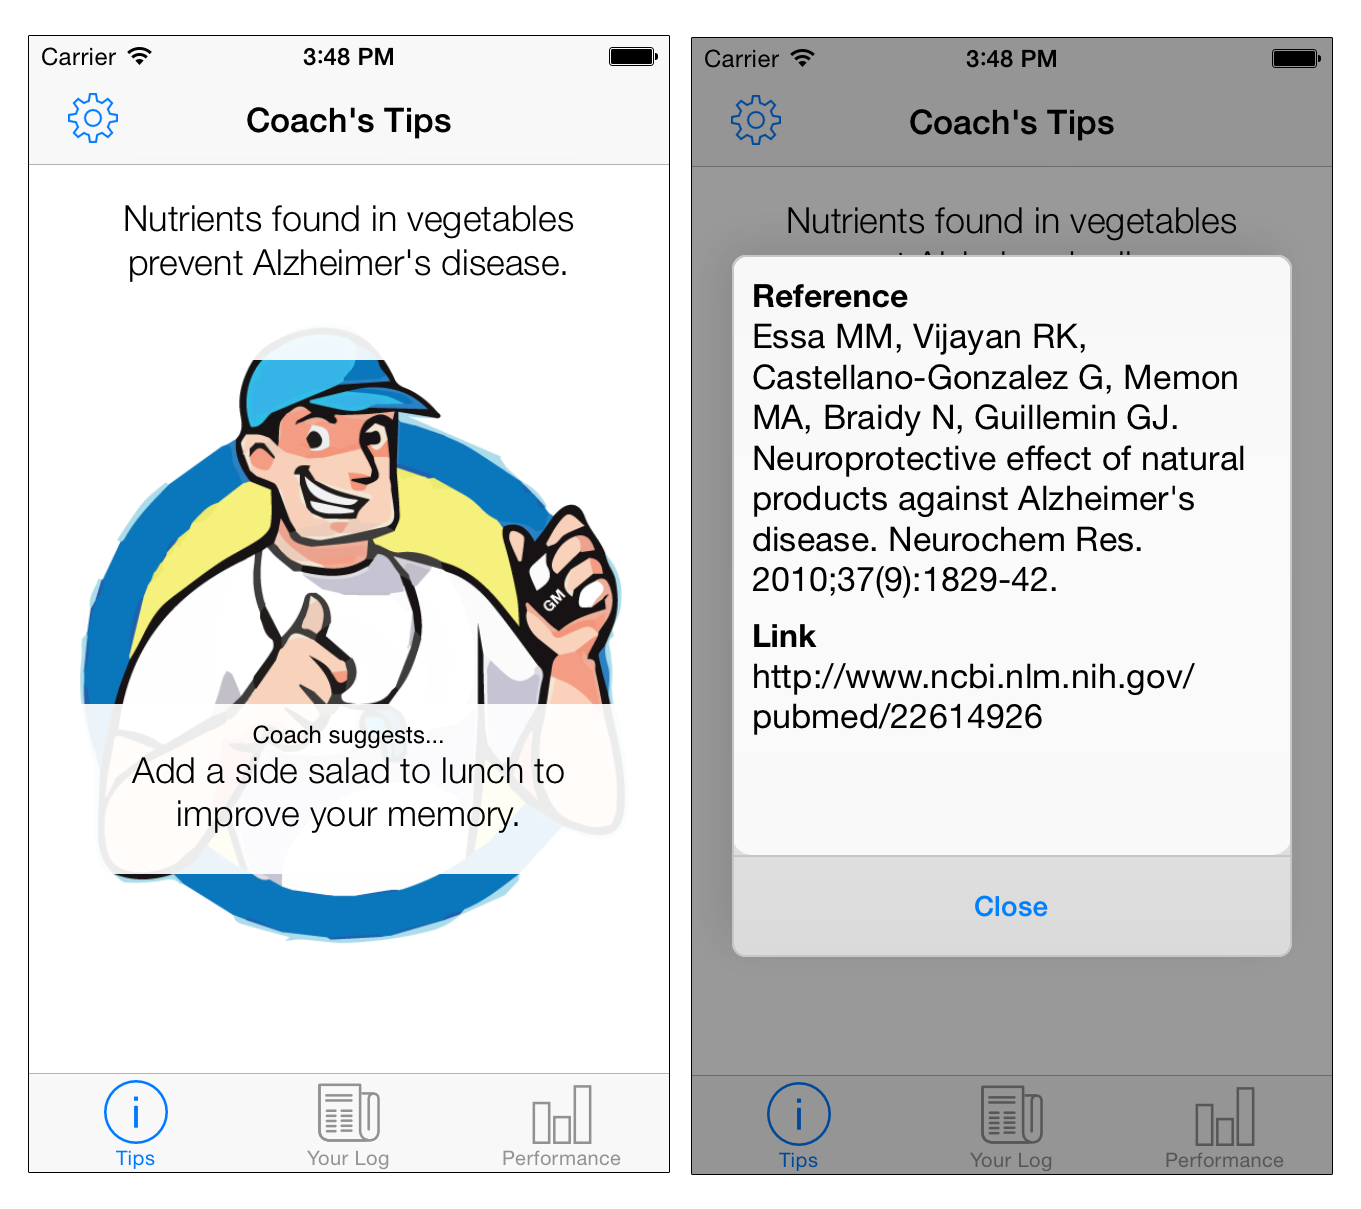
\includegraphics[scale=0.25, angle=0]{Files/prevention-study-1/figures/screenshot-dailyfact.png}
    \caption{Screenshot of app showing daily fact tab. Daily fact is accompanied by a coach avatar, which when tapped presents information on the supporting literary evidence.}
    \label{fig: screenshot-dailyfact}
\end{figure}

\subsubsection{Learning favourable behaviours}
To assess behaviour change for each domain, a number of questions were designed to be presented to the user each day (specific information for each question is detailed in Section \ref{subsection-montoringcomponent}). In addition to being a method to gain insight into user behaviours, the questions also aim to educate the user about the quantity and quality of certain behaviours through self-assessment. Users can view what the recommended target is for each behaviour type, report their own behaviour and immediately understand their relative performance. Through this repetitive daily process, users become educated about ideal targets and methods to achieve them.

\subsection{Behaviour Monitoring Component} \label{subsection-montoringcomponent}
The monitoring component of the app is designed to allow the user to perform various processes of the TTM, including consciousness raising, self-re-evaluation and reinforcement management. For an individual to effectively modify their behaviour, they should understand what their current behaviour is and what their ideal or target behaviour should be. To do this, the app provides a mode which allows the user to report their behaviours relevant to AD risk on a daily basis.

\subsubsection{Facilitating self-reporting}
For each of the identified domains, daily questions were developed and refined from the list of key measures (Table \ref{tbl: key-measures}), to capture behaviours relevant to AD risk. These questions were designed by a team of researchers from the Family, Consumer, and Human Development department at Utah State University \cite{Norton2015-TRCI}. All questions were quantitative in nature, however, contained a mixture of subjective and objective questions. For example, a user may be asked to report the number of fruits and vegetables they consumed in a day (objective), and also rate their quality of sleep on a scale of 0-10 (subjective).
In addition to the questions for the original 6 behavioural domains, a question was added to collect any activity data observed via a user's wearable activity monitor. In total 12 questions were designed for the domains: Physical (2), Diet (3), Social (1), Sleep (1), Cognitive (2) and Stress (2) and Wearable Activity Monitor (1). For each question, a recommended daily target value was extracted from external knowledge sources, such as the World Health Organisation (WHO), the American Heart Foundation (AHF), and the Centre for Disease Control and Prevention’s (CDC). Full details of these questions can be found in Table \ref{tbl: questions}.

\begin{sidewaystable}[ph!]
\centering
\caption{Questions presented to the user, showing their minimum, maximum and recommended values.}
\label{tbl: questions}
\resizebox{23cm}{!}{%  begin resize to fit text
\begin{tabular}{lllllll}
\toprule
Domain                     & Id & Question                                                                         & Min. & Max. & Recommended     &  \\ \midrule
\multirow{2}{*}{Cognitive} & 1  & How many minutes did you spend today doing ``novel mental exercises''?             & 0    & 120  & 30 minutes      &  \\
                           & 2  & How many minutes did you spend today doing ``cognitively stimulating activities''? & 0    & 120  & 30 minutes      &  \\ \midrule
\multirow{3}{*}{Diet}      & 3  & How many cups of fruits and vegetables did you eat today?                        & 0    & 10   & 5 cups          &  \\
                           & 4  & How many ounces of whole grains did you eat today?                               & 0    & 10   & 3 ounces        &  \\
                           & 5  & How many servings of nuts, seeds, or legumes did you eat today?                  & 0    & 5    & 1 serving       &  \\ \midrule
\multirow{2}{*}{Physical}  & 6  & How many minutes of ``moderate'' physical activity did you do today?               & 0    & 60   & 30 minutes      &  \\
                           & 7  & How many minutes of ``vigorous'' physical activity did you do today?               & 0    & 60   & 20 minutes      &  \\ \midrule
Sleep                      & 8  & How would you rate your sleep promotion efforts over the past 24 hours?          & 0    & 5    & 5 (out of 5)    &  \\ \midrule
Social                     & 9  & How would you rate your social engagement in the last 24 hours?                  & 0    & 7    & 7 (out of 7)    &  \\ \midrule
\multirow{2}{*}{Stress}    & 10 & How much effort have you put into decreasing your stress over the past 24 hours? & 0    & 10   & 10 (out of 10)  &  \\
                           & 11 & On a scale of 1-10 how would you rate your stress level over the past 24 hours?  & 1    & 10   & 1 (out of 10)   &  \\ \midrule
Wearable                   & 12 & How many Nike Fuelpoints did you earn today?                                     & 0    & 5000 & 2000 Fuelpoints &  \\ \bottomrule
\end{tabular}
} % end resizebox
\end{sidewaystable}

The recommended value serves 3 key purposes:
\begin{enumerate}[noitemsep,topsep=0pt]
\item to act as an \textbf{observable goal} for the user.
\item to efficiently \textbf{calculate performance} of a user.
\item to \textbf{compare performances} of other users.
\end{enumerate}

Further information of calculating performance is detailed in Section \ref{subsubsection-calculating-performance}.

\subsubsection{Data Entry}
Data entry for each question is facilitated by a bespoke list view, that uses a draggable sliding bar to allow quick and accurate entry of information. A screenshot of the listview containing several questions is presented in Figure \ref{fig: screenshot-measure}. Each list item contains a fixed-width slider bar, with a draggable circle that moves on the horizontal plane. As the circle moves from left-to-right, the value increments by a set value, typically by 1. Displaying progress as a bar that grows on the horizontal plane provides the user immediate visual feedback toward their current progress. The maximal value achievable for each slider is typically double the recommended value, allowing users to overachieve their targets and give recognition to their efforts (reinforcement management).

\begin{figure}[h]
    \centering
    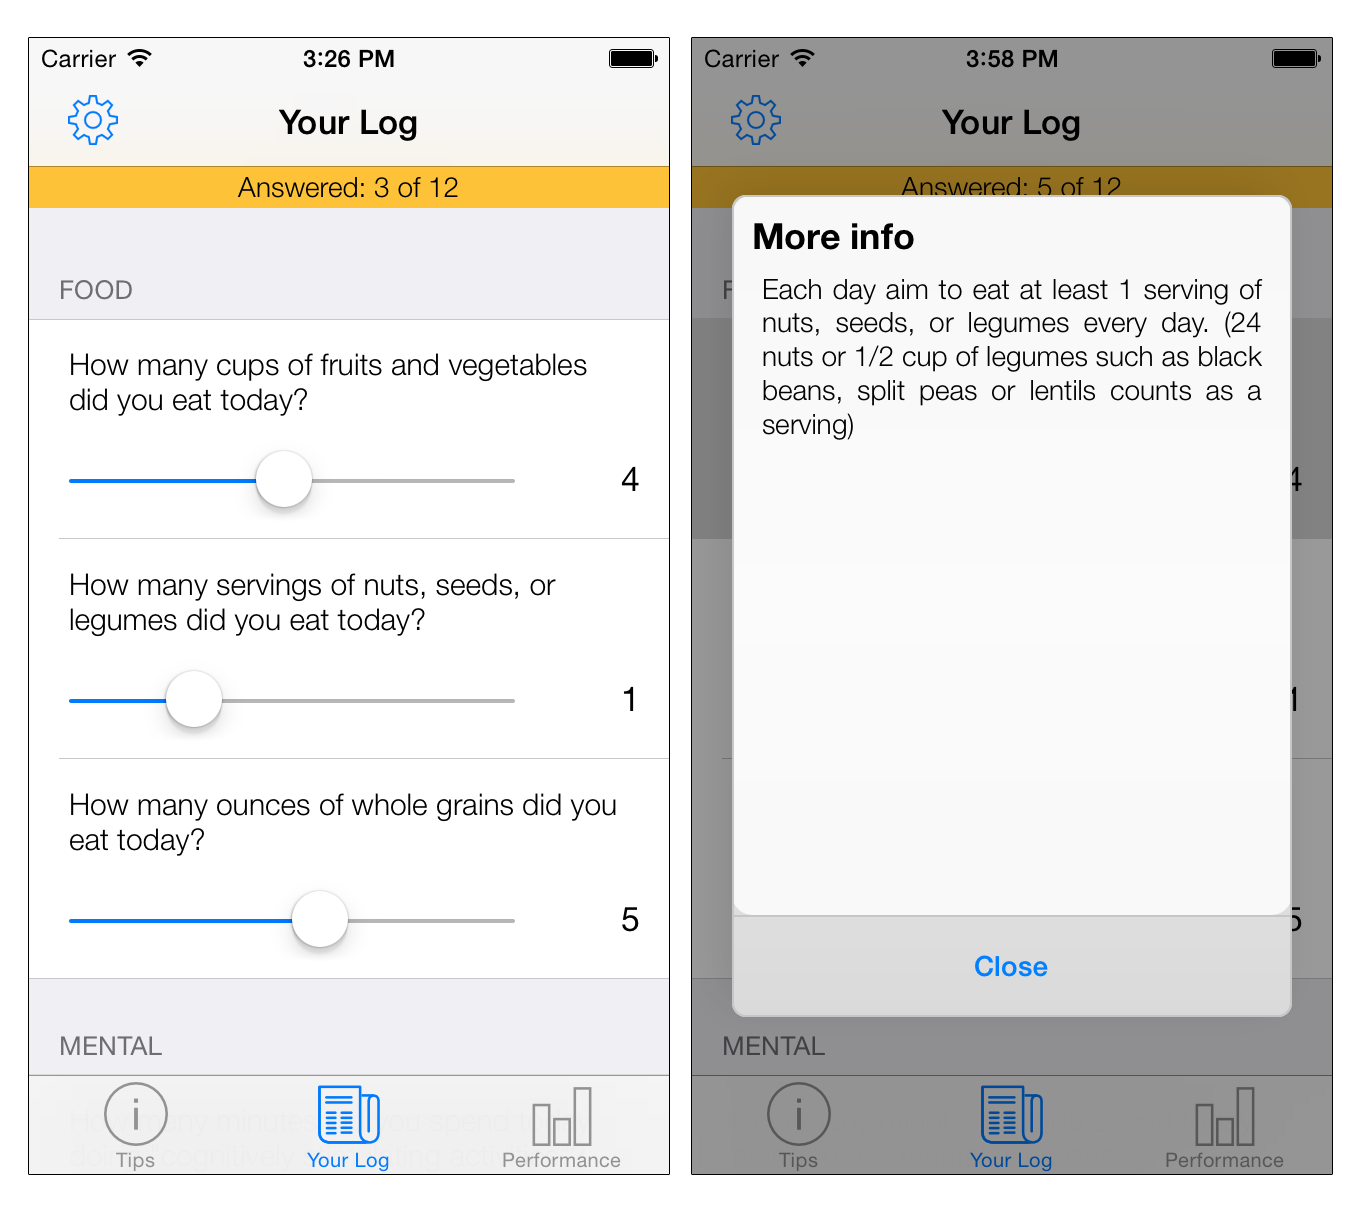
\includegraphics[scale=0.25, angle=0]{Files/prevention-study-1/figures/screenshot-measure.png}
    \caption{Screenshot of app showing self-reporting screens and supporting information. User entered their values via the slider bars.}
    \label{fig: screenshot-measure}
\end{figure}

\subsubsection{Improving Question Interpretation}
To assess behaviour change for each domain, a number of questions are designed to be presented to the user. Each question seeks to measure information about a user's behaviours longitudinally, both in a qualitative and quantitative manner. In order for these measurements to remain accurate, the user must understand what the question is asking, how they can measure it, and what the favourable result is. Therefore, the user must be educated on the topic on which they are being queried.
For example, the question:
\begin{displayquote}
\textit{``How many servings of nuts, seeds, or legumes did you eat today?"}
\end{displayquote}
may elicit confusion for a number of reasons. Firstly, the user may not know the existence of certain food items. Secondly, the user may also be unsure as to what constitutes a \textit{`serving'} of the items, or how many servings are favoured.
To address these issues, the app provides descriptions of all of these areas which may lead to potential uncertainty for the user. To access additional information for any question or behaviour, the user simply taps the question which presents a modal dialog box, as presented in Figure \ref{fig: screenshot-measure}. Ensuring that all users understand the question is vital for comparisons of self-reported behaviours across multiple users.

\subsection{Feedback Component}
The feedback component of the app is designed primarily to motivate the user through to self-re-evaluation, reinforcement management and also via established gamification techniques.

\subsubsection{Gamification}
Motivation plays a key role in all models of behaviour change. Maintaining motivation is difficult over time, and may people relapse to their prior behaviours, simply because they no longer feel motivated to progress. Gamification involves turning typically mundane tasks into a form of game, utilising a variety of methods commonly found in game playing, such as points earning, competition and reward systems \cite{Deterding2011a}. All of these game mechanics have been found to encourage continual engagement, and subsequently progression in various studies \cite{Hamari2014}. Gamification is a relatively new concept, and its use to encourage behaviour change in adults is relatively limited. Nevertheless, initial findings show that it can be applied successfully in health care promotions to maximise engagement \cite{Schoech2013}. Therefore, within this study, points earning elements of gamification have been implemented as a mechanism by which users may be encouraged to achieve their daily recommended targets.
%VIVA: If asked can you offer altertantive approaches and justify why the approach you have adopted is best?

Upon entering data for a question, the user can view their relative performance for that domain in the performance tab. Each topic is shown in a listview, accompanied by a number of achievable stars. The stars are designed to encourage and reinforce a participant’s effort to change their behaviour. Since all domains can be viewed on screen at the same time, it provides a fast method to deliver visual feedback on the domains that require more effort \cite{Hartin2015-JMIR}. An example of the visual elements implemented to represent progress are presented in Figure \ref{fig: screenshot-performance}.
\begin{figure}[h]
    \centering
    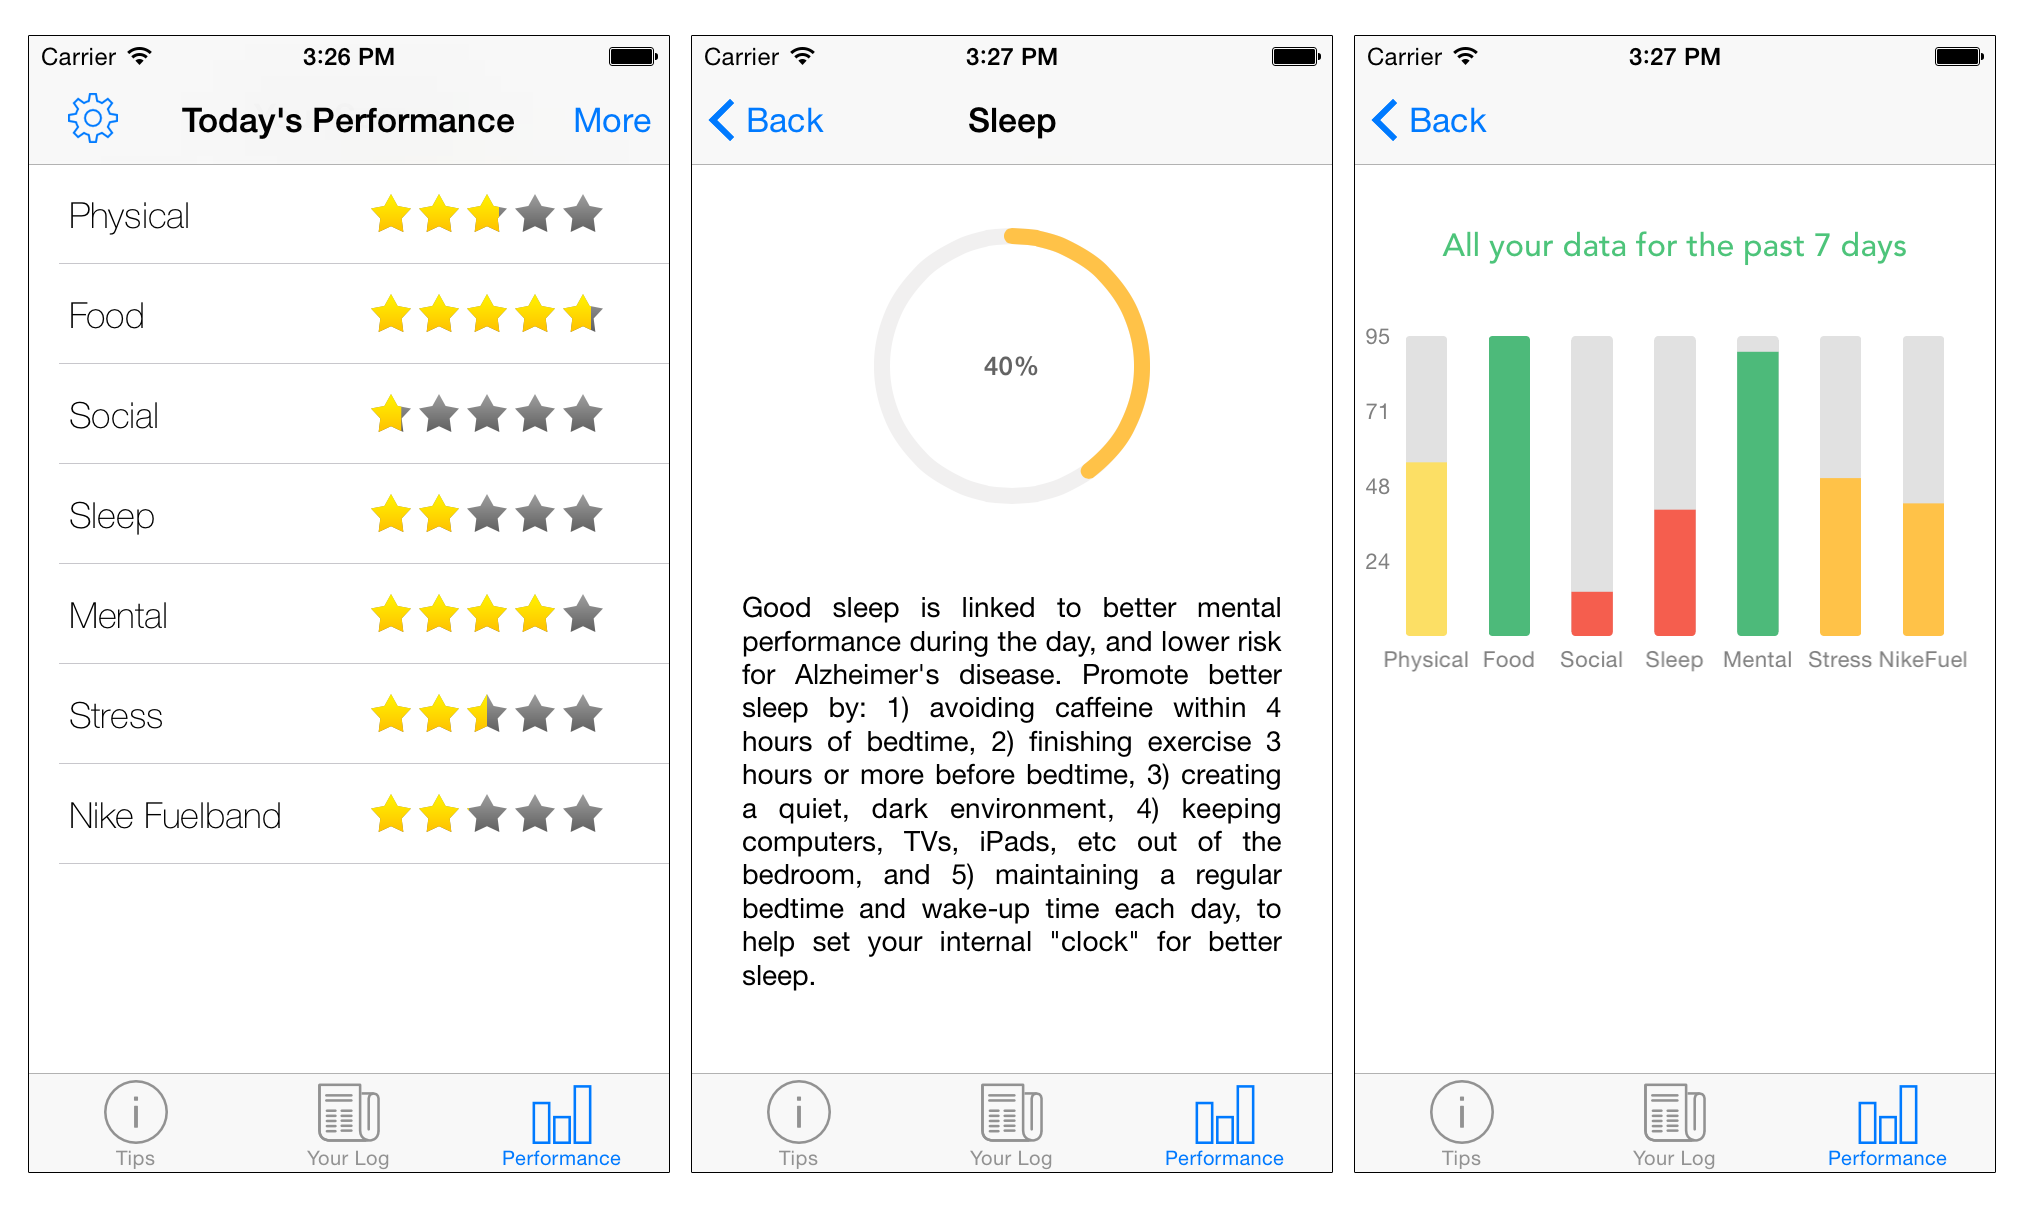
\includegraphics[scale=0.2, angle=0]{Files/prevention-study-1/figures/screenshot-feedback.png}
    \caption{Screenshots of app showing high-level and longitudinal feedback on reported behaviours. The app utilises a variety of graphical representations of progress, stars, animated filling circles and bar charts.}
    \label{fig: screenshot-performance}
\end{figure}

Users may also tap upon each domain to display an information screen, providing additional pertinent material about that domain with a further graphical representation of their efforts. In this same screen, users are provided with additional tips and methods by which they could improve their performance. For example, in the sleep domain, tips include:
\begin{enumerate}[noitemsep,topsep=0pt]
\item Avoid caffiene within 4 hours of bedtime.
\item Keep computers, TVs, iPads etc, out of the bedroom.
\item Maintaining a regular bedtime and rise time each day will help set your internal clock for better sleep.
\end{enumerate}

All tips and further information developed can be found in Appendix \ref{apndx: domain-tips}.

The users may also view their performance aggregated across the previous 7 days in the form of a bar chart or spider diagram, as presented in Figure \ref{fig: screenshot-performance}. Again this serves to visually assist the participants in understanding their behaviours longitudinally for the purpose of self-affirmation and reinforcement management, discussed in the processes of the TTM.

\subsubsection{Calculating Performance} \label{subsubsection-calculating-performance}
Using the concepts explored in gamification, the user can achieve a maximum of 5 stars for each behavioural domain each day. To receive the full 5 stars for a domain, the user must achieve the recommended values for all the behaviours within that domain (refer to Table \ref{tbl: questions}). Given that many of the behaviours are reported across various fixed value ranges, the values must be normalised to within a range of 0 - 5 in relation to the recommended value \cite{Hartin2014-IWAAL}. This is achieved via the following function developed by the author
\begin{equation}
f(x) = \left\{
         \begin{array}{l l}

         R_{U} & \quad
           \text{if }{x \geq Q_{G} }\\

           \frac{
           \left(x-Q_{L}\right)\times\left(R_{U}-R_{L}\right)}
           {Q_{G}-Q_{L}}
           + R_{L} & \quad
           \text{if }{Q_{L} \leq x < Q_{G}}\\

          \end{array}
          \right.
          \label{eq: calc-performance-stars}
\end{equation}

where $x$ is the user’s answer value to a particular question, $Q_{G}$ is the goal value for the question, $Q_{L}$ is the lowest possible value for that question, $R_{U}$ is the upper boundary of the normalised result and $R_{L}$ is the lowest boundary.

\subsection{Usage Component}
This component of the framework involves the monitoring of the user's interactions with the app for the benefit of the developers and health investigators.
Using a mixture of proprietary and open-source analytical tools \cite{Hartin2014-IWAAL,GoogleAnalyticsWeb,MixpanelAnalytics}, it is possible to inject traceable hooks into any aspect of the app's code base. Within this app, the following actions were identified to be tracked via analytic code:
\begin{itemize}[noitemsep,topsep=0pt]
\item Launching the app.
\item Navigating screens.
\item Updating behaviours.
\item Seeking additional detail for topics/questions.
\item Seeking additional detail for performance.
\item Changing notification times.
\end{itemize}

Observing these actions will allow the developer to further understand the needs of the end-user without direct communication. This can be performed in a number of ways: by measuring which actions are the most commonly used within the app, observing the typical screen flow of users and assessing if users are getting stuck at specific points in the app. Observing seemingly arbitrary user actions such as changing notification times can provide insight into the average or preferred times, which subsequently would be made the default parameters upon the apps install for new users.
Additional useful information can be gleaned by combining this app usage data, with the behavioural data reported by the user. From this combination, observations can be made to establish which user, or user types, benefit most from the system in its current version and also identify those who may require additional support.
%VIVA: You may address this later in the thesis,  however,  at this stage it seems a bit vague as to why you are recording what you are recording.

\subsection{Data Component}
The data component controls the storing and uploading of the user's behaviours, both self-reported and extracted from app usage for the benefit of the health investigators. Health investigators, those facilitating the behaviour change intervention, are interested in observing trends, making predictions and detecting anomalies. Therefore, the integrity and accessibility of the data is vitally important to this party, particularly if analyses are to be carried out mid-intervention. The networking model implemented for this framework is a centralised client-server model, whereby a number of clients access a single networked server. This is illustrated in Figure \ref{fig: clientserver-model}.

\begin{figure}[h]
    \centering
    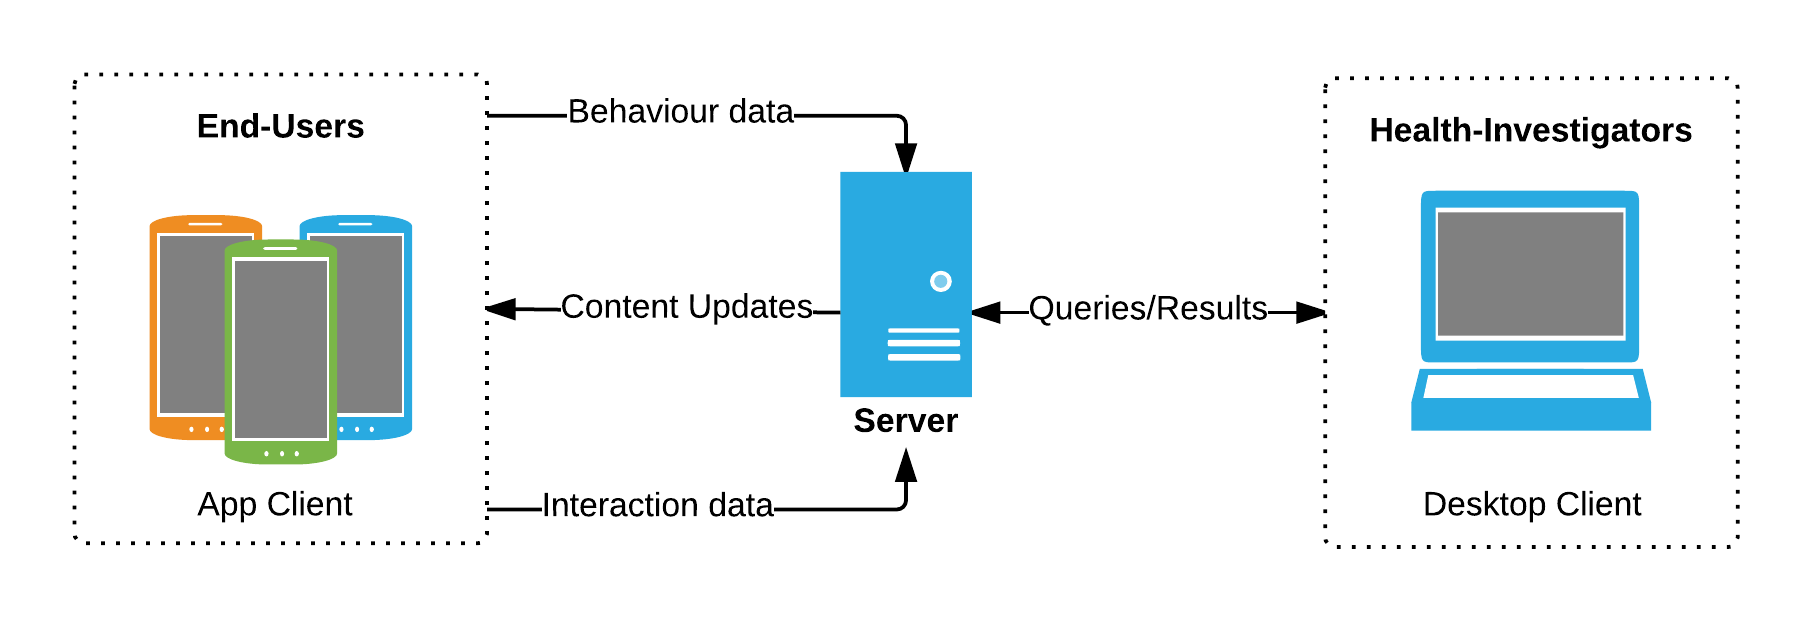
\includegraphics[scale=0.9, angle=0]{Files/prevention-study-1/figures/client-server}
    \caption{Centralised Client-Server Network Model.}
    \label{fig: clientserver-model}
\end{figure}

\subsubsection{Uploading Data}
Upon installation of the app on a smartphone, a local database is created to contain app specific data. This data is intermittently uploaded to the central server. Data only flows between the client (app) and the server. Data cannot be directly shared between clients, i.e. from one installation of the app to another, without first being processed and authenticated by the central server (Further detail regarding protocols are discussed in Section \ref{subsection-api}).

\subsubsection{Downloading Data}
Since the scientific evidence is forever evolving on AD risk factors and prevention methods, the information that the app is packaged with should not be considered final. All information displayed to the user via the app can be updated from the central server. This includes the daily facts, the language used in the behavioural questions, their supplementary descriptions, and the feedback text in the performance tabs. Upon a change to any of this material on the central database, a global version number is updated. The app will frequently check if its local version number matches the global version number on the central server. If an app detects that the local version number is outdated, the app will pull the changes from the server and update its local database.

\section{Business Logic Implementation}
The application server performs the majority of the business logic involved within this system, including the registration of participants, handling authentication, controlling access to the intervention material, and aggregation of participant data. The server runs a variant of the open-source linux operating system, contains a number of statistical software packages and hosts a relational database management system (RDBMS). Since the app relies heavily upon the transfer of data between client and server via the internet, an application programming interface (API) was developed to facilitate these functions through the methods outlined in representational state transfer (REST) architecture \cite{Fielding2000, Benslimane2008}. This is further illustrated at a high-level in Figure \ref{fig: clientserver-model-detail}.

\begin{figure}[h]
    \centering
    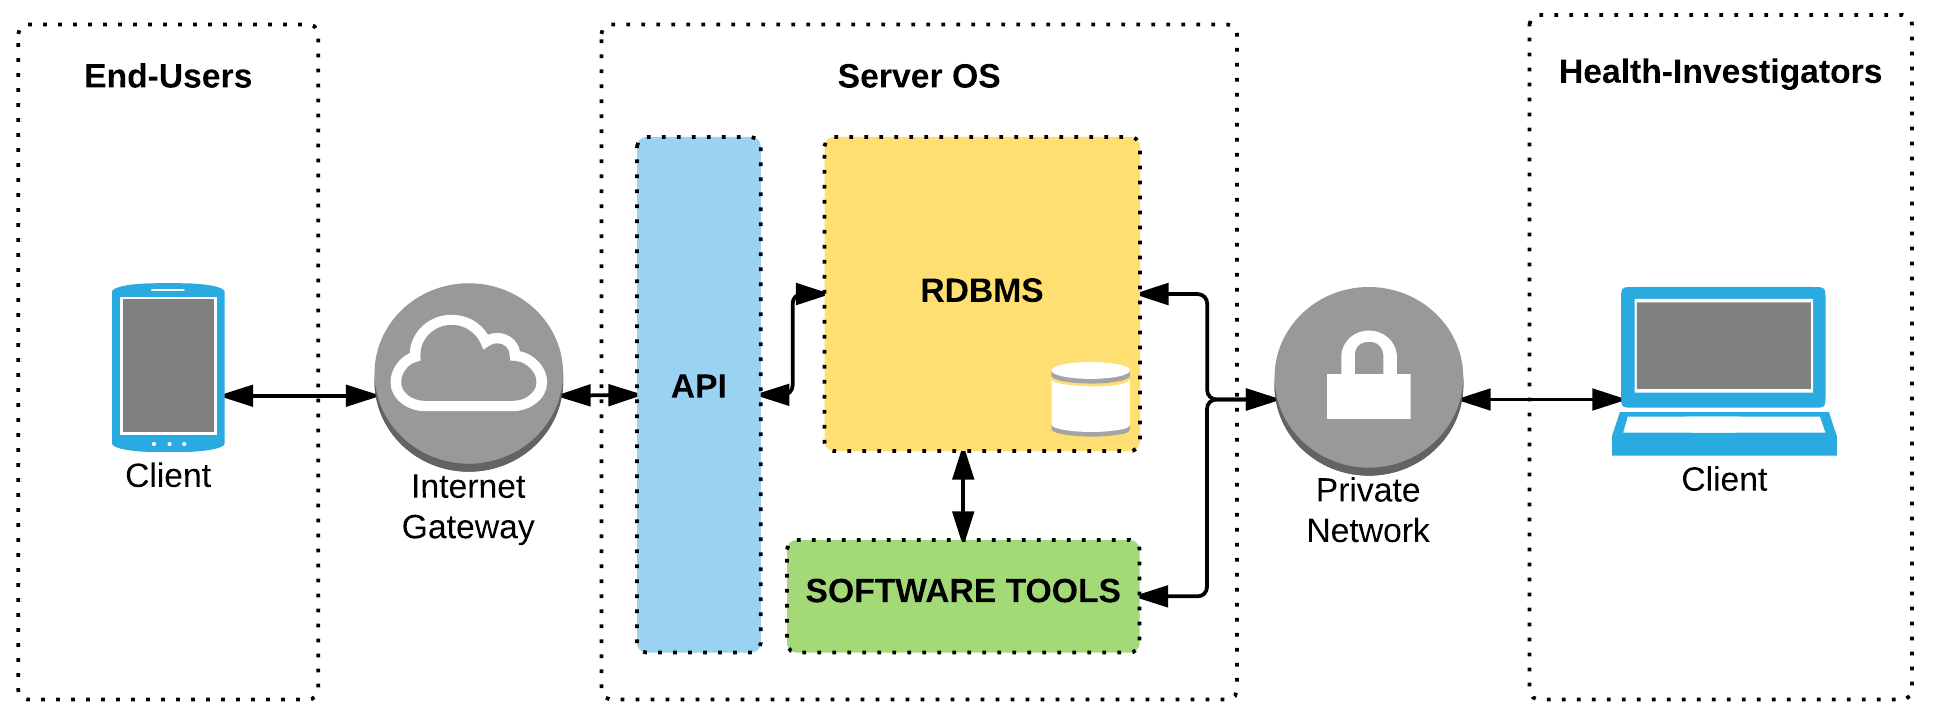
\includegraphics[scale=0.9, angle=0]{Files/prevention-study-1/figures/client-server-adapted}
    \caption{High-level Server Architecture Overview. HI and end users alike gain access to server via their respective protocols. HI have the ability to run analytical software locally on the server, whereas end users simply interface with the defined API.}
    \label{fig: clientserver-model-detail}
\end{figure}

\subsection{Database Schema}
The database schema describes the structure, format and relationships between the models in the RDBMS. In this system, various components of the app have been re-modelled for the act of persistence and storage on the servers RDBMS. Figure \ref{fig: database-model} shows these models in further detail. Using the same models throughout the client and the server development dramatically improves development overheads, reduces the risk of type-mismatches, and enables reflection of objects across the Android and iOS platforms \cite{Thalheim2000}.
\begin{figure}[h]
    \centering
    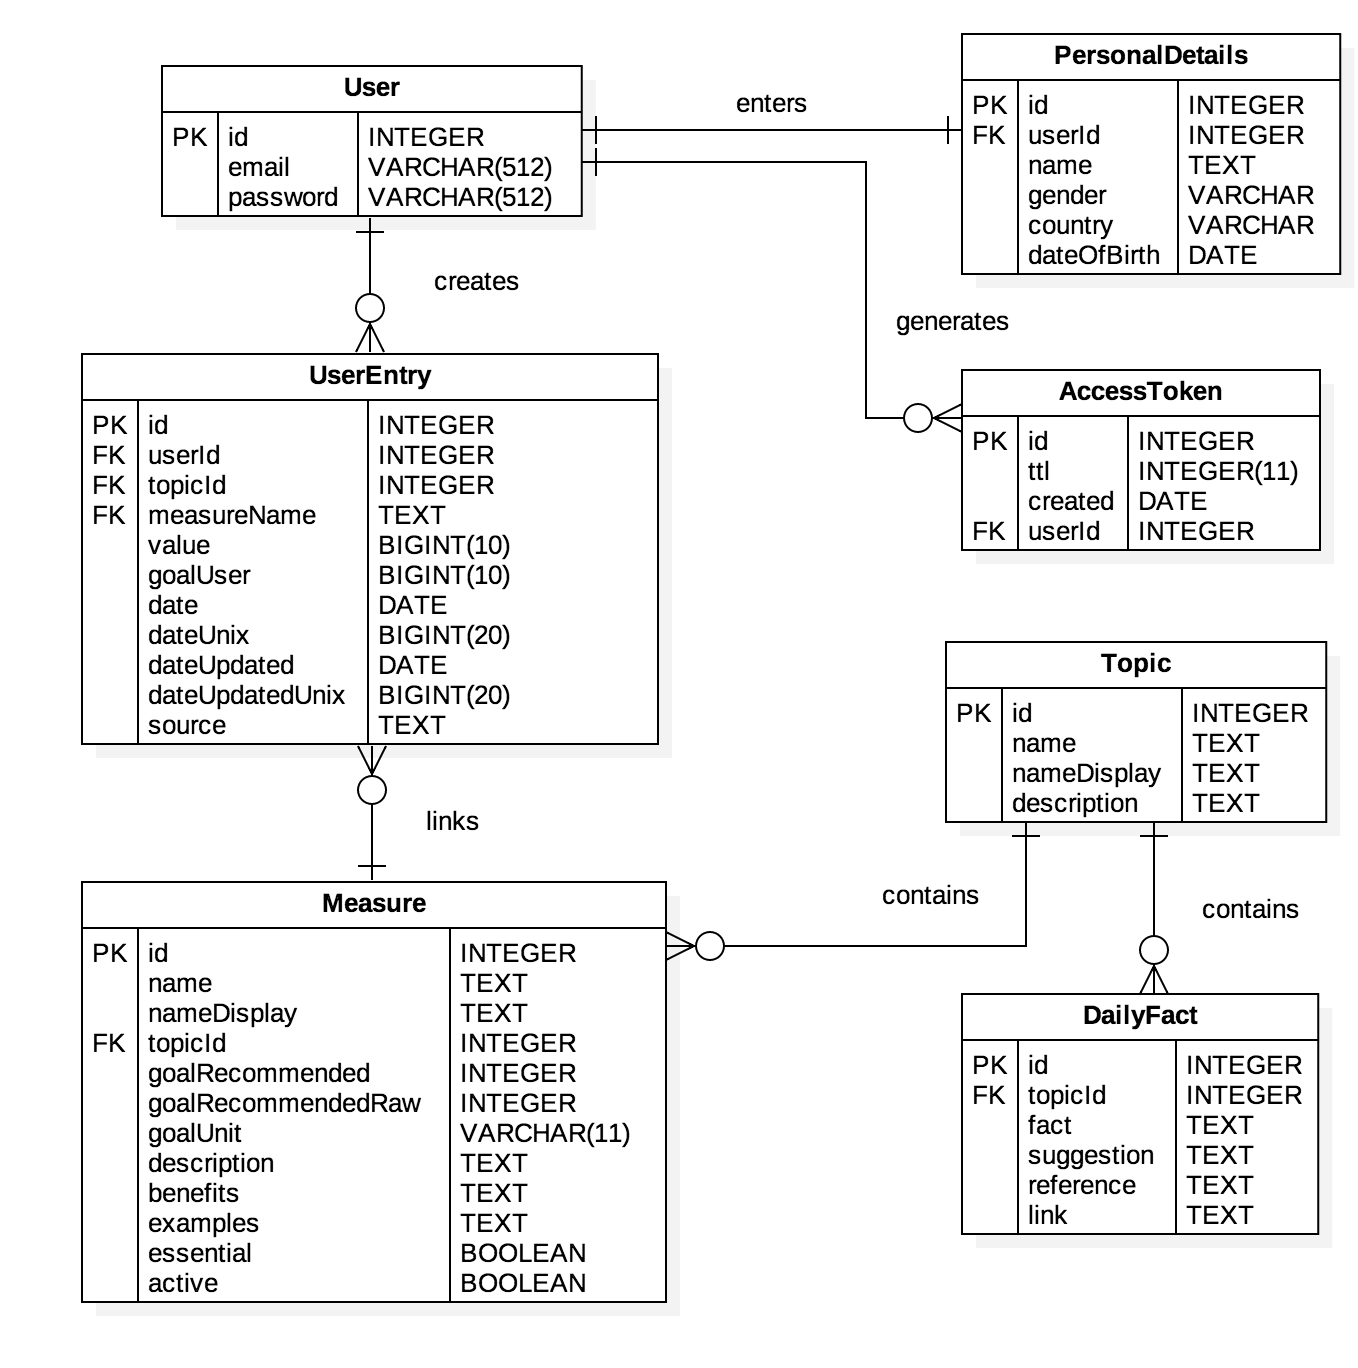
\includegraphics[scale=0.3, angle=0]{Files/prevention-study-1/figures/database-model}
    \caption{The data schema for object models utilising database relationships.}
    \label{fig: database-model}
\end{figure}
%VIVA: How does this schema relate to the earlier proposed ERD of one person has a disease, many risk etc.

\subsubsection{Exposing models through a RESTful API} \label{subsection-api}
With a well-defined and stable data model, it is possible to expose certain aspects of the model via an API. The creation of an API allows controlled interaction between the server and its clients, through a set of defined methods and routines. With the goal of keeping the data model intact on the central server, implementing strict protocols within the API is very beneficial. In this use-case, potential client's operating systems will be varied (iOS, Android). As such, their platform specific languages and data-models can also vary, however, the API requires that all data transmitted conforms to its protocols. Using a language independent notation, such as JSON (JavaScript Object Notation), enforces system-wide validity of transmitted data, which is of paramount importance to the health-investigators study analyses. Descriptions of the API objects, their JSON structure and example data are detailed in Appendix \ref{apndx: rest-objects}.

\subsection{Monitoring Participants}
A large advantage of an internet orientated architecture is the readiness of data. In real-time, the HI can view when a user updates a behavioural log, enabling immediate (re)analysis of the data. The HI can perform queries on the RDBMS, through a private, protected network. To further improve the usability of the server for the HI, numerous methods were developed to aid the automation of data aggregation and statistical analysis. This analysis could be performed at an individual, or cohort level.
Examples include analysing the relationships between internal components (daily facts, behaviour suggestions, app usage) and external components of the study (time of day, local weather, current events). Results of such analysis are explored in Chapter \ref{chapter: prevention-rctresults}.

\section{Conclusion}
This Chapter has described an evidence based framework, including process guide, from which to base the development of technology driven behavioural change intervention. The Chapter also demonstrated a use-case of the framework, in its application to AD. The resulting app and its technical specifications are also detailed. Expert assessment of the app can be found in the following Chapter, and the clinical and behavioural outcomes through use of the app can be found in Chapter \ref{chapter: prevention-rctresults}.
 % 4 GM Framework
\chap{Evaluation of Implementation through Expert Review} \label{chapter: prevention-evaluation}

\epigraph{The most important property of a program is whether it accomplishes the intention of its user.}{\textit{Charles Antony Richard Hoare}}

This chapter details the results of a series of assessments of the developed Gray Matters app. Ranging from expert review to content analysis, the app and it's components are critically evaluated. These evaluations result in the exposure of common attributes amongst successful apps, which influence future recommendations of various software elements and approaches.

\section{Introduction}
Following the process outlined in Section \ref{subsection: framework-process}, the developed solution should be peer-reviewed by domain experts using a suitable objective method. Academically recognised approaches for the assessment of mHealth apps are very limited, however, the previously mentioned MARS \cite{Stoyanov2015} tool is a suitable scale by which the Gray Matters app can be evaluated.

\section{Mobile App Rating Scale}
The MARS tool provides an established method by which to rate an app across 4 objective criteria: Engagement, Functionality, Aesthetics, and Information. The scale also includes an additional subjective quality assessment criteria. 23 individual criterion are presented to the reviewer in total, each relating to a specific criteria, and a mean score is generated for each. A summary score, referred to as the MARS mean score, is calculated as the the mean score across the 4 objective criteria (excluding the subjective quality criteria scores). This is the primary measure by which all apps are contrasted or ranked.
In the development of the MARS framework, the authors identified 59 mHealth (mobile health) apps that were available to the public via their platforms respective app stores. Of these 59, 9 were randomly selected to develop the scale in a pilot study, and 50 were subsequently used to evaluate the consistency and inter-reliability of the scale.

\subsubsection{Potential Limitations}
Whilst the MARS framework provides a suitable set of objective questions, and displayed excellent internal consistency, a number of limitations with the MARS framework were observed.

\textbf{Stress Domain Focused.}
The original rating scale was developed during a pilot study, by reviewing 9 apps, of which only 1 addressed more than one behavioural domain. A large proportion of these apps, 66.7\%, were primarily aimed at reducing stress, whilst the remainder addressed diet, sleep and social domains. No apps addressed physical activity, diet, or smoking.

\textbf{Excludes N/A Ratings.}
Within the information criteria rating scale, questions aim to score various aspects of the information provided, e.g., quality, quantity, graphical representation etc. This is performed by rating these sub-categories from 1-5. The highest rating of 5 denotes that the information is correct, clear and concise. The lowest rating of 1, however, is reserved for irrelevant or incorrect information. There is no figure that denotes a lack of information, or no information. The framework states that if this occurs, that they should be marked `N/A' for not applicable, and these should be excluded when calculating the mean information score. This is problematic for a number of reasons.
Many mHealth and educational apps attempt to deliver information in a number of formats, using text, audio, video and graphs. If an low quality app does not deliver any information, yet scores highly due to matching the marketplace description, it is possible to score a higher mean score, despite providing less information. An illustrative example of this can be seen in Table \ref{tbl: information-rating-illustration}.

\begin{table}[]
\centering
\caption{Example of N/A label bias on mean information score}
\label{tbl: information-rating-illustration}
\resizebox{\textwidth}{!}{%
\begin{tabular}{@{}cclllllll@{}}
\toprule
 & \multicolumn{1}{m{2.3cm}}{\centering App Description Accuracy} & Goals & Quality & Quantity & Visual & Credibility & Evidence & \multicolumn{1}{m{1.2cm}}{\centering Mean Score} \\ \midrule
App A       & 3                        & 3     & 4       & 3        & 3      & 1           & N/A      & {\it 2.83} \\
App B       & 5                        & N/A   & N/A     & N/A      & N/A    & 1           & N/A      & {\it 3.00} \\ \bottomrule
\end{tabular}
}
\end{table}

\textbf{Disciplinary Bias.}
In the pilot study, the apps were reviewed by 2 expert raters from the field of psychology. Upon examining the distribution of scoring from the pilot study, as seen in Figure \ref{fig: mars-pilot-histogram}, indicates that most apps scored above the scales natural mean point of 2.5. \begin{figure}[t]
    \centering
    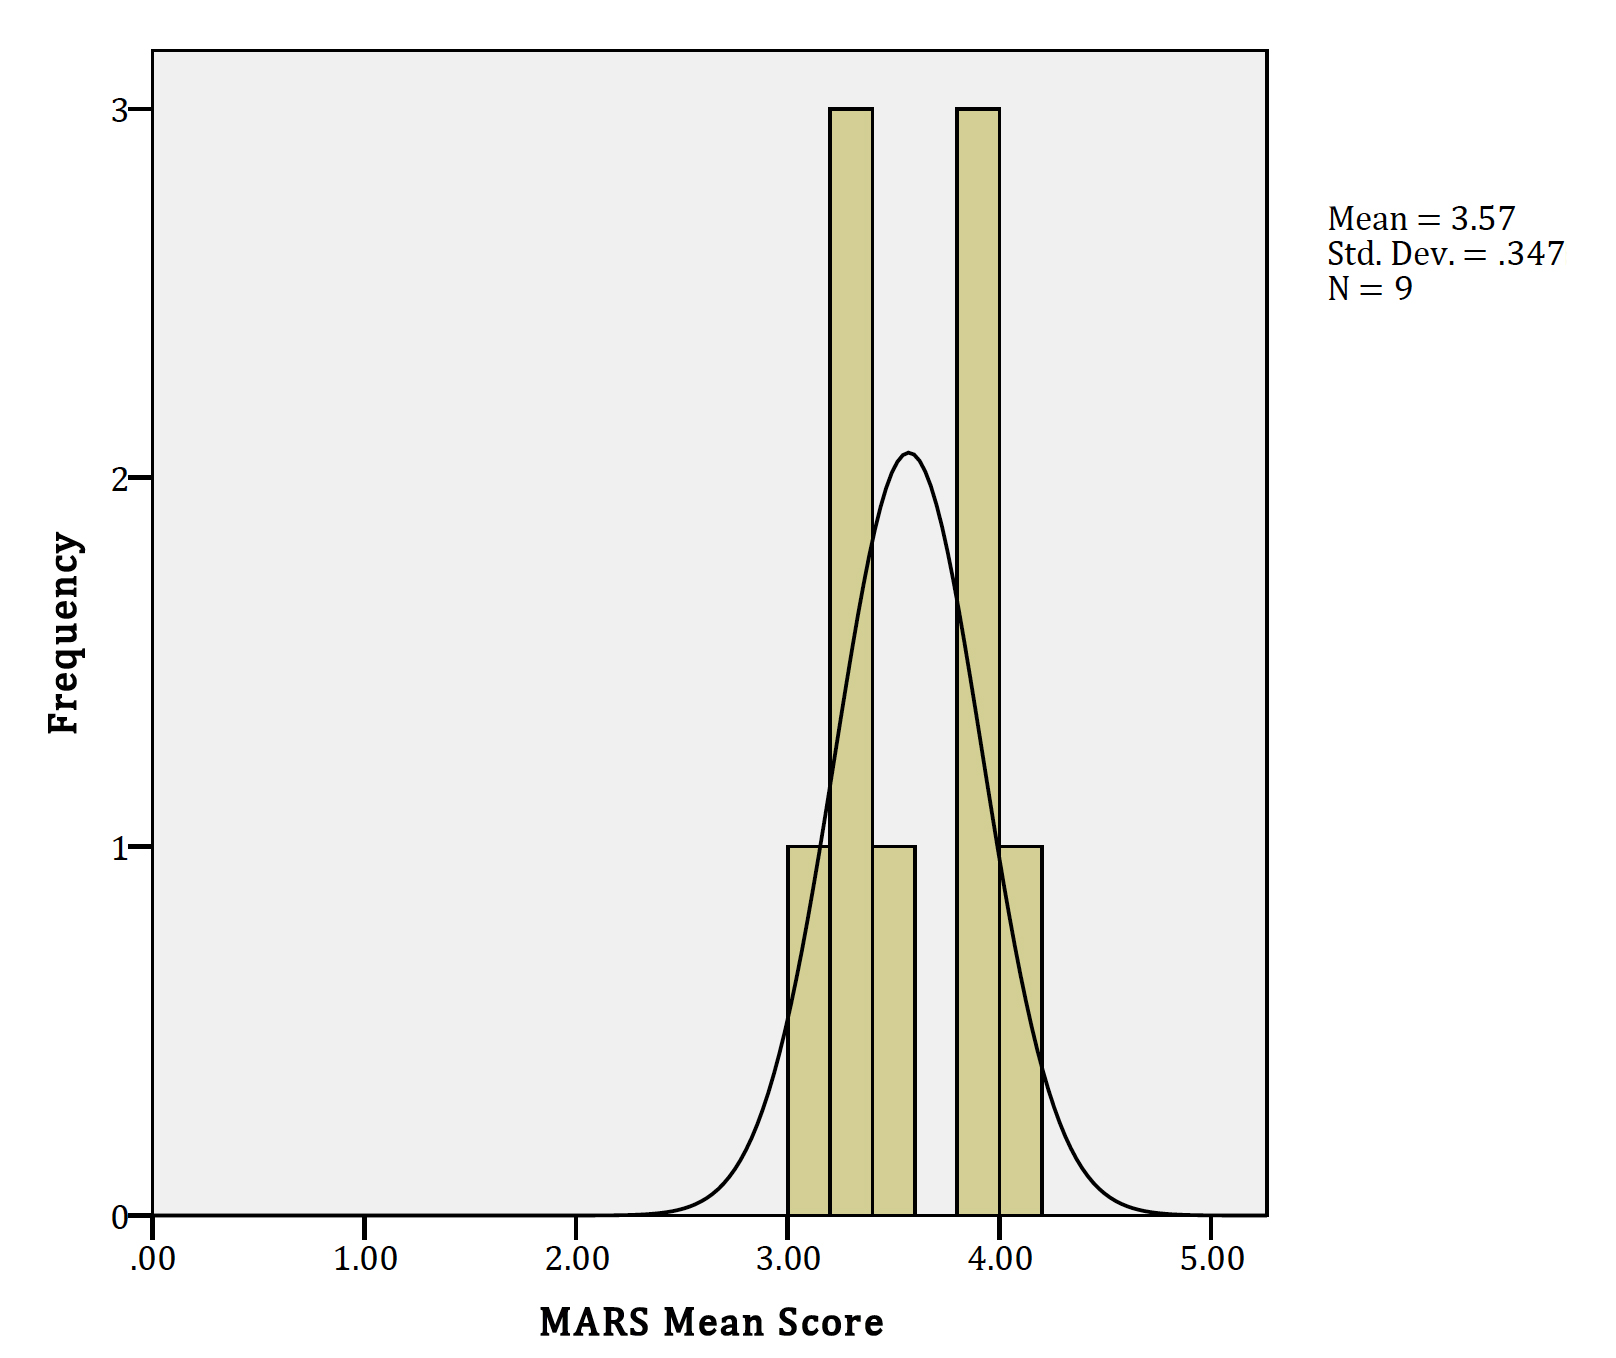
\includegraphics[scale=0.20, angle=0]{Files/prevention-study-2/figures/mars-pilot-histogram}
    \caption{Histogram showing distribution and normal curve of mean scores in initial MARS Pilot study}
    \label{fig: mars-pilot-histogram}
\end{figure}
This hinted that cognitive bias may exist in the results, perhaps stemming from non-technologists scoring technology solutions highly due to lack of domain knowledge. The authors do state however that one reviewer has 9 years experience with information technology \cite{Stoyanov2015}, although the exact details of their proficiency was not stated.

\subsubsection{Testing for Disciplinary Bias}
To ensure this cognitive bias did not exist, the same 9 apps used to develop the MARS scale were evaluated by the author, a PhD candidate in the Computer Science domain. Following the protocol of the original study \cite{Stoyanov2015}, all 9 apps were downloaded onto their respective platforms, used for approximately 10 minutes, and scored. The full assessment results sheet can be seen in Appendix \ref{apndx: mars-pilot-reevaluation}.

The authors of the original study disclosed the criteria scores for each app, allowing for a detailed comparison. The resulting MARS scores from the pilot and the re-evaultion performed by the author can be seen in Table \ref{tbl: MARSpilot-vs-author}.

\begin{table}[h]
\centering
\caption{MARS scores of initial 9 apps from Pilot study, as marked by original study and author}
\label{tbl: MARSpilot-vs-author}
\resizebox{\textwidth}{!}{%
\begin{tabular}{@{}llll@{}}
\toprule
App & Score (MARS Pilot) & Score (Author) & Difference \\ \midrule
Breathe Daily & 3.91         & 3.75          & .16        \\
Everyday	Health with Acupressure & 3.52         & 3.63          & -.11       \\
Interpersonal Dynamics & 3.94         & 3.90          & .04        \\
iPhoria Nature's Music & 3.74         & 3.53          & .21        \\
iThoughtjournal & 3.65         & 3.51          & .14        \\
Meditation Seconds Lite & 3.71         & 3.48          & .23        \\
Personal	 Remedies & 3.77         & 3.59          & .18        \\
Sleep Easily              & 3.90         & 3.81          & .09        \\
We Breathe & 3.90         & 3.75          & .15        \\ \bottomrule
\end{tabular}
}
\end{table}

A number of tests were performed to measure the reliability of the authors scoring, following methods outlined in \cite{McHugh2012}. Intraclass correlation coefficient (ICC) using Cronbach's alpha was performed on the scores from both assessments, resulting in a correlation coefficient of .852, as seen in Table \ref{tbl: intraclass-pilot-reevaluation}. A consistency of 85.2\% between the original study and the re-evaluation performed by the author is high, and notably higher than the ICC of .79 from the original MARS study \cite{Stoyanov2015}. This finding supports the original study's claim that the scale has excellent consistency and inter-rater reliability \cite{Stoyanov2015}. It is therefore presumed that the remaining 50 apps would be marked similarly, despite variation in the expert rater's discipline. This assumption is tested again, later within this chapter.

\begin{table}[h]
\centering
\caption{Intraclass Correlation Coefficient for Pilot vs Re-evaluation}
\label{tbl: intraclass-pilot-reevaluation}
\resizebox{\textwidth}{!}{%
\begin{tabular}{@{}llllllll@{}}
\toprule
\multicolumn{1}{c}{} & \multicolumn{1}{c}{\multirow{2}{*}{\begin{tabular}[c]{@{}c@{}}Intraclass \\ Correlation \textsuperscript{\textit{b}}\end{tabular}}} & \multicolumn{2}{c}{95\% CI} & \multicolumn{4}{c}{F Test with True Value 0} \\ \cmidrule(l){3-8}
 & \multicolumn{1}{c}{} & Lower & Upper & Value & df1 & df2 & Sig \\ \midrule
Single Measures & .742 \textsuperscript{\textit{a}} & .206 & .935 & 6.740 & 8 & 8 & .007 \\
Average Measures & .852 \textsuperscript{\textit{c}} & .342 & .967 & 6.740 & 8 & 8 & .007 \\ \bottomrule
\end{tabular}
}
\end{table}

\section{Recruitment}
The Gray Matters app was publicly demonstrated during the Technology and Dementia symposium at the 2015 Alzheimer's Association International Conference in Washington, D.C \cite{AlzheimersAssociation2015}. During this event, a number of physicians, pharmacologists, psychologists and technologists were interested in the app's potential use cases. Interested parties were given access to an online version of the MARS tool from which they could complete the survey. In addition, a number of technology researchers from the Smart Environments Research Group at the University of Ulster were also permitted to complete the survey.

\section{Assessment Scores}
As of January 2016, 5 expert raters have reviewed the app using the MARS tool. These raters are from 2 relevant disciplines, Medicine (n=4) and Computer Science (n=1). It must be noted that the expert raters in both fields have had professional experience in psychology and/or the study of behaviour change.
Each rater was asked to download the app and use for 5-10 minutes. After use of the app, the rater was asked to complete the MARS survey. The rater could reuse the app during the completion of the survey to minimise information recall error. The descriptive statistics of the Gray Matters app ratings can be seen in Table \ref{tbl: gm-expert-ratings}

\begin{table}[h]
\centering
\caption{Descriptive statistics of expert raters scoring for each assessment category, and total means, including and excluding subjectivity}
\label{tbl: gm-expert-ratings}
\begin{tabular}{@{}llllll@{}}
\toprule
Criteria      & N & Minimum & Maximum & Mean   & Std. Deviation \\ \midrule
Engagement    & 5 & 3.80    & 4.40    & 4.1200 & .30332         \\
Functionality & 5 & 4.25    & 4.75    & 4.5000 & .17678         \\
Aesthetics    & 5 & 4.67    & 5.00    & 4.7360 & .14758         \\
Information   & 5 & 4.29    & 4.71    & 4.4860 & .18783         \\
Subjective    & 5 & 3.25    & 4.00    & 3.6000 & .37914         \\
MARS Score    & 5 & 4.31    & 4.60    & 4.4580 & .14307         \\
True Mean     & 5 & 4.10    & 4.47    & 4.2880 & .17513         \\ \bottomrule
\end{tabular}
\end{table}

\textbf{MARS Score.}
The app received a mean overall MARS score of 4.45 $\pm$ .14.

\textbf{Engagement.}
The app received a mean engagement score of 4.12 $\pm$ .30.

\textbf{Functionality.}
The app received a mean functionality score of 4.5 $\pm$ .176.

\textbf{Aesthetics.}
The app received a mean aesthetics score of 4.73 $\pm$ .147.

\textbf{Information.}
The app received a mean information score of 4.48 $\pm$ .187.

\textbf{Subjective.}
The app received a mean score of 3.6 $\pm$ .379.
As to be expected the subjectivity score shows the greatest degree of standard deviation, hence it's naming.

\textbf{True Mean (Including Subjective).}
The app received a true mean score of 4.28 $\pm$ .121. This score is lower than the official MARS score which does not account for the subjective criteria. The difference between the MARS score (M = 4.45, SD = 0.30) and True Mean (M = 4.28, SD = .121) score was found to be statistically significant in a paired samples t-Test at the p \textless 0.05 level [t(4) = 6.292, p = 0.03].

\subsection{Discussion}
The app scored very highly in all areas. A mean MARS score of 4.45 ranks the Gray Matters app 2\textsuperscript{nd} out of 60 reviewed apps (59 Original + Gray Matters app). When comparing the true mean scores (including subjective score), the app also ranks 2\textsuperscript{nd}. The nearest ranking app in both cases is `headspace', a structured meditation guide which launched in 2010 \cite{HEADSPACE}. Headspace is marketed as \textit{`a gym membership for the mind}', and aims to reduce stress and increase mindfulness for its' users. The app has over 5 million installs on android devices alone. If the MARS score is indicative of public adoption, the resulting Gray Matters app demonstrates the framework's promise as an mHealth development platform.

\textbf{Ensuring validity.}
Whilst the results of the expert review are encouraging, steps must be taken to ensure that these ratings were valid and comparable to the original study. To do this, each expert was asked to rate an app from the original MARS study, and from a list of newly sourced apps. In the following sections, the inter-rater reliability and ICC scores for each expert are established. 

\section{Comparison with Existing Apps}
Whilst the MARS scale has produced an average rating of 4.45 across 5 expert reviewers, the score exists without true context. It is important to compare this result with that of existing apps, which are aiming for similar outcomes. As such, a number of apps within the area of quantified-self and health improvement were considered for review.

\subsection{Existing App Review Data}
As noted earlier, the apps reviewed in the MARS pilot (n=9) were predominately focused on the stress domain. In the full MARS study, an additional 50 apps were included in the assessment of the scale. The original authors disclosed the criteria scores and mean MARS score for each of these 50 apps. These apps were then targeted for inclusion in a comparison with the Gray Matters app. However, initial content analysis of the apps found that a 13.5\% (n=8) were not relevant to behaviour change in any of the identified domains, or they did not aim to improve health outcomes. As such these 8 were excluded from further study. Of the remaining apps (n=51), the behavioural focus was heavily unbalanced, with 74.5\% (n=38) of the apps focusing strictly on the stress domain. In addition, no apps reviewed in the original MARS studies addressed smoking, and only 1 targeted the social domain. As such it was apparent that additional apps should be reviewed to provide a fairer and representative comparison of existing apps in the marketplace.

\subsection{Identifying Suitable Apps}
Identifying suitable apps to compare to the developed solution is difficult. The Gray Matters app is a disease specific app, utilising education delivery and behaviour tracking across numerous behavioural domains. The Gray Matters app is itself a relatively novel concept, thus narrowing the number of potential apps from which to compare. There are however a large number of apps that focus on specific behavioural areas, such as cognitive stimulation, diet monitoring, activity tracking, activity promotion and stress relief. There are also a number of apps that aim to disseminate information on Alzheimer's Disease and other areas of cognitive decline.

Suitable apps for comparison were identified by searching the iOS and Android marketplaces for apps that that met the following criteria:
\begin{itemize}[noitemsep,topsep=0pt]
\item Encouraged behaviour change
\item Aimed to improve health status
\item Gamified behaviour change
\item Delivered condition specific health education
\end{itemize}

This search reviewed over 70 publicly available apps, of which 36 where identified as suitable for comparison. The distribution of primary behavioural domains targeted by these additional apps can be seen in Table \ref{tbl: app-dataset-frequencies}. The inclusion of these apps does help to balance the distribution of domains targeted from the original study, however, stress remains the most frequently targeted domain (47.1\%).

\begin{table}[h]
\centering
\caption{Comparison of app datasets and distribution of primary behavioural domain targeted}
\label{tbl: app-dataset-frequencies}
\begin{tabular}{@{}lllllll@{}}
\toprule
\multirow{2}{*}{Domain} & \multicolumn{2}{l}{MARS} & \multicolumn{2}{l}{App Market} & \multicolumn{2}{l}{Consolidated} \\ \cmidrule(l){2-7}
                        & n        & \%            & n           & \%               & n          & \%              \\ \midrule
Physical                & 4        & 7.8\%         & 8           & 22.2\%           & 12         & 13.8\%          \\
Diet                    & 2        & 3.9\%         & 7           & 19.4\%           & 9          & 10.3\%          \\
Cognitive               & 2        & 3.9\%         & 7           & 19.4\%           & 9          & 10.3\%          \\
Sleep                   & 4        & 7.8\%         & 3           & 8.3\%            & 7          & 8.0\%           \\
Social                  & 1        & 2.0\%         & 4           & 11.1\%           & 5          & 5.7\%           \\
Stress                  & 38       & 74.5\%        & 3           & 8.3\%            & 41         & 47.1\%          \\
Smoking                 & 0        & 0.0\%         & 4           & 11.1\%           & 4          & 4.6\%           \\ \midrule
Total                   & 51       & 100.0\%       & 36          & 100.0\%          & 87         & 100.0\%         \\ \bottomrule
\end{tabular}
\end{table}

\subsection{Ensuring Reliability}
All 36 apps were analysed and reviewed by the author. As established earlier, the authors ICC is .852, showing excellent consistency with the original study. To further validate the scores that were attributed by the author, each expert rater, in addition to rating the Gray Matters app, where asked to rate an additional 3 apps:
\begin{enumerate}[noitemsep,topsep=0pt]
\item Two from the original MARS list \cite{Stoyanov2015}.
\item One from the additional 36 apps identified by the author.
\end{enumerate} 

A measure of inter-rater reliability, or concordance, was calculated between the expert reviewers and the original study reviewer, and also between the expert reviewers and the author. These measures seek to justify the ratings reached by the experts in their review of the Gray Matters app.

\subsubsection{Method}
Each expert rater was asked to review two apps from the original study \cite{Stoyanov2015} and one from the additional 36 apps added by the author. A random number generator was used to select the app ids. The 3 apps highlighted for review were: PTSD Coach (MARS), Conscious (MARS), Water Your Body (Extra). The scores reached by each expert rater, including the original MARS scores and authors re-evaluation, can be seen in Table \ref{tbl: expert-vs-author-apps}.

\begin{table}[h]
\centering
\caption{MARS scores attributed by each expert rater, the original study, and the author}
\label{tbl: expert-vs-author-apps}
\resizebox{\textwidth}{!}{%
\begin{tabular}{@{}llllllll@{}}
\toprule
                & MARS & Expert 1 & Expert 2 & Expert 3 & Expert 4 & Expert 5 & Author \\ \midrule
PTSD Coach      & 4.29 & 3.1      & 3.26     & 3.63     & 3.1      & 3.12     & 3.1    \\
Conscious        & 3.36 & 2.93     & 3.38     & 3.26     & 3.15     & 3.3      & 3.15   \\
Water Your Body & N/A   & 3.7      & 3.77     & 4.11     & 3.96     & 3.85     & 3.96   \\
Gray Matters    & N/A   & 4.31     & 4.48     & 4.59     & 4.31     & 4.6      & N/A     \\ \bottomrule
\end{tabular}
}
\end{table}

\subsubsection{Expert Review and Original MARS Reliability}
Using the MARS scores from the original study and the scores from the expert reviews, a reliability analysis was performed. Descriptive statistics, detailing means and standard deviations for each rater are displayed in Table \ref{tbl: expert-vs-mars-apps-descriptive}. 

\begin{table}[h]
\centering
\caption{Expert rater and MARS statistics}
\label{tbl: expert-vs-mars-apps-descriptive}
\begin{tabular}{@{}llll@{}}
\toprule
          & Mean   & Std. Deviation & N \\ \midrule
Expert 1  & 3.0150 & .12021         & 2 \\
Expert 2 & 3.3200 & .08485         & 2 \\
Expert 3 & 3.4450 & .26163         & 2 \\
Expert 4 & 3.1250 & .03536         & 2 \\
Expert 5 & 3.2100 & .12728         & 2 \\
MARS      & 3.8250 & .65761         & 2 \\ \bottomrule
\end{tabular}
\end{table}

In this instance, we can see that Expert 1 attributes the lowest mean scores across the reviewed apps (n=2), whilst the original MARS score has the highest mean and largest standard deviation. The differences between the MARS score and the experts seems significant. Reliability analysis performed using SPSS v22 confirms this, showing an ICC of .167. This suggests poor consistency between the experts and the original MARS study. It appears that the MARS studies results may be the cause of this. To test, reliability analysis was performed between the expert ratings of all apps (n=4), omitting the MARS results. The ICC between the expert raters was found to be .991, displaying excellent consistency. 

\subsubsection{Expert Reviewers and Author Reliability}
The expert review scores were then compared against the authors scores. Descriptive statistics, detailing means and standard deviations for each rater are displayed in Table \ref{tbl: expert-vs-author-apps-descriptive}. 

\begin{table}[h]
\centering
\caption{Expert rater and author statistics based on MARS scores}
\label{tbl: expert-vs-author-apps-descriptive}
\begin{tabular}{@{}llll@{}}
\toprule
Rater      & Mean   & Std. Deviation & N \\ \midrule
Expert 1   & 3.2767 & .39068         & 3 \\
Expert 2 & 3.5667 & .18448         & 3 \\
Expert 3 & 3.7733 & .29670         & 3 \\
Expert 4  & 3.4367 & .45391         & 3 \\
Expert 5  & 3.4567 & .34298         & 3 \\
Author     & 3.4033 & .48274         & 3 \\ \bottomrule
\end{tabular}
\end{table}

Again we can see that Expert 1 attributes the lowest mean scores across all apps (n=3), whilst the author has the largest observed standard deviation. The differences are minor, as the average rate of agreement between all raters, based on the ICC using Cronbach's alpha, is 97.6\% (ICC .976, p = \textless .000). This displays excellent consistency and suggests that the expert raters and the author can produce reliable judgement in the absences of the other. This is in stark contrast to the rate of agreement found between the expert reviewers and the original study.

\subsubsection{Discussion}
The results from the reliability analysis of the author and the original MARS pilot study are encouraging, as are the results from the author and the expert reviews. The reliability found between the experts and the original MARS study however indicate that certain issues exist. There are a number of possible reasons for the observation: 

\textbf{Sensitivity.}
The number of apps from which the comparisons were made were very small (n=2). Cronbach’s alpha can be very sensitive to the number of items involved, as noted by \citeauthor{Clark1995} \cite{Clark1995}. As such, for future comparisons an larger number of apps should be reviewed to find a more representative result.

\textbf{Profession Bias.}
Given that the expert reviewers were predominately from the medical domain, profession or knowledge bias may of affected the results. Future tests aim to include additional experts from varying fields.

\textbf{App Evolution.}
The original MARS study was performed in 2014, using apps which were popular at the time. The standard of app has since increased, both aesthetically and functionally. As such, these older apps when reviewed by todays standards may score much lower. This effect is particularly apparent for PTSD Coach, and can be seen in Table \ref{tbl: expert-vs-author-apps}. 

\subsection{Ranking}
Using the mean expert rating of 4.45, the Gray Matters app is ranked 3\textsuperscript{rd} of the 87 apps reviewed, and is placed in the first decile (\textgreater 4.29). A histogram displaying the distribution of all 87 apps MARS scores can be seen in Figure \ref{fig: allapps-histogram}. Figure \ref{} also shows the distibution of MARS scores based upon the app's source, i.e. The Original MARS study or additional 36 apps added.

\begin{figure}[h]
    \centering
    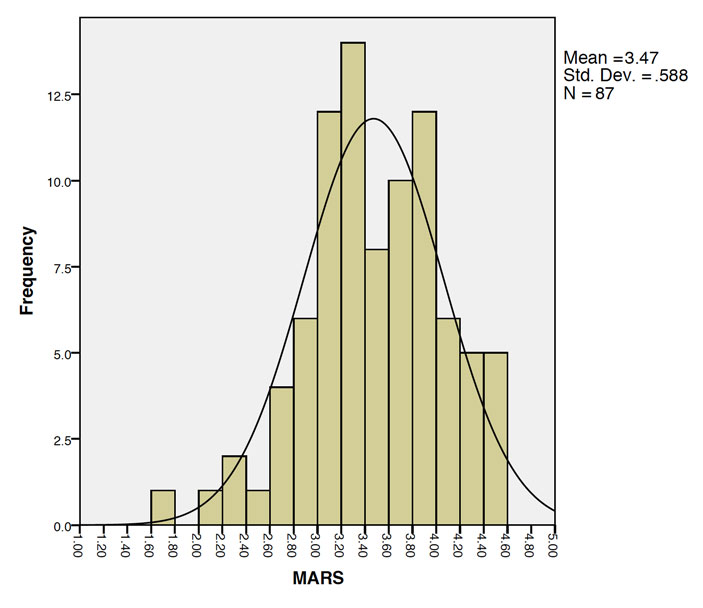
\includegraphics[scale=0.4, angle=0]{Files/prevention-study-2/figures/allapps-histogram}
    \caption{Histogram showing distribution and normal curve of mean MARS scores for all 87 reviewed apps}
    \label{fig: allapps-histogram}
\end{figure}

\begin{figure}[h]
    \centering
    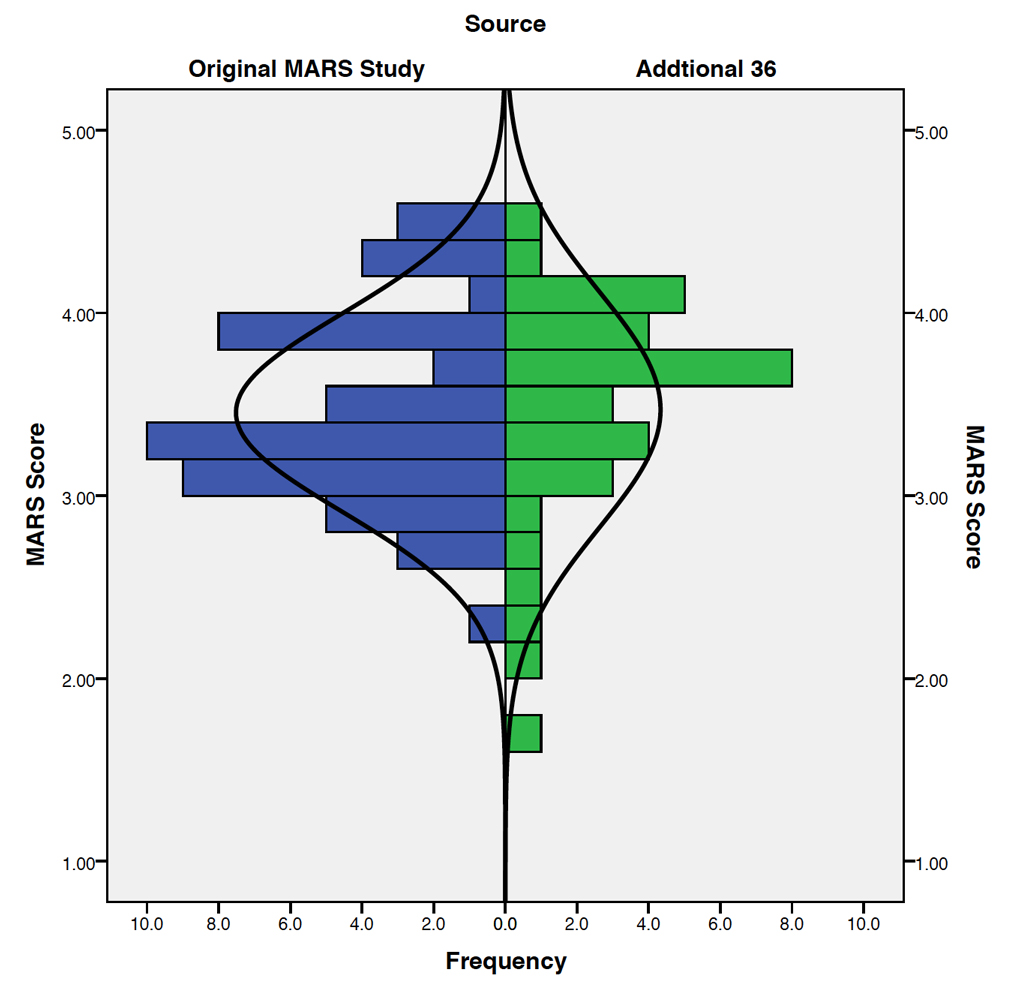
\includegraphics[scale=0.30, angle=0]{Files/prevention-study-2/figures/allapps-histogram-bysource}
    \caption{Histogram showing distribution and normal curve of mean MARS scores for all 87 reviewed apps segregated by source}
    \label{fig: allapps-histogram}
\end{figure}

Whilst the apps can be ranked against one another using the MARS score, the reasons for the score are still not fully understood. To understand the factors which influence the rankings content analysis is performed on all 87 apps.

\section{Content Analysis} \label{subsection: content-analysis}
All 87 apps were downloaded, used, and studied by the author to glean information as to the various approaches used. This included establishing the primary behavioural domain targeted, if multiple domains were addressed, the format of educational information, the method of behavioural tracking (if applicable), if behavioural goals were recommended and if progression was structured/guided.

Correlation and regression analysis was performed on all observed content. Correlation analysis was used to determine if there was a relation between two or more variables, and to what degree. Regression analysis was used to establish if one variable (i.e. Number of domains addressed) could predict the outcome of another (i.e. MARS score). In addition, analysis of variance (ANOVA) was used to determine if there was a significant difference in results between two or more independent groups (e.g. Educational format used and Mean Education score).

\subsection{Domains Targeted}
%Pairs of domains targeted commonly found together?
Apps were analysed to establish which behavioural domains they targeted. In cases where an app targeted more than 1 domain, a primary domain was established. Descriptives of this analysis can be seen in Table \ref{tbl: descriptive-primarydomain-mars}. A count of targeted domains was also calculated.

\begin{table}[h]
\centering
\caption{Descriptive statistics of MARS score by primary domain targeted}
\label{tbl: descriptive-primarydomain-mars}
\begin{tabular}{@{}lllllllll@{}}
\toprule
 &  &  &  &  & \multicolumn{2}{l}{95\% CI for Mean} &  &  \\ \cmidrule(lr){6-7}
\begin{tabular}[c]{@{}l@{}}Primary\\ Domain\end{tabular} & N & Mean & \begin{tabular}[c]{@{}l@{}}Std. \\ Dev.\end{tabular} & \begin{tabular}[c]{@{}l@{}}Std. \\ Error\end{tabular} & \begin{tabular}[c]{@{}l@{}}Lower\\ Bound\end{tabular} & \begin{tabular}[c]{@{}l@{}}Upper\\ Bound\end{tabular} & Min. & Max. \\ \midrule
Physical & 12 & 3.7017 & .46501 & .13424 & 3.4062 & 3.9971 & 3.01 & 4.45 \\
Diet & 9 & 3.7322 & .51558 & .17186 & 3.3359 & 4.1285 & 3.09 & 4.49 \\
Cognitive & 9 & 3.3967 & .96903 & .32301 & 2.6518 & 4.1415 & 1.67 & 4.51 \\
Sleep & 7 & 3.1514 & .29311 & .11079 & 2.8803 & 3.4225 & 2.73 & 3.53 \\
Stress & 41 & 3.4561 & .51771 & .08085 & 3.2927 & 3.6195 & 2.22 & 4.49 \\
Social & 5 & 2.9420 & .79408 & .35513 & 1.9560 & 3.9280 & 2.00 & 3.90 \\
Smoking & 4 & 3.7775 & .29590 & .14795 & 3.3067 & 4.2483 & 3.43 & 4.11 \\ \midrule
Total & 87 & 3.4731 & .58904 & .06315 & 3.3476 & 3.5986 & 1.67 & 4.51 \\ \bottomrule
\end{tabular}
\end{table}

One-way ANOVA was used to compare the effect of the primary domain targeted on the MARS score. ANOVA analysis showed there was no significant effect of the primary domain on the MARS Score at the p\textless.05 level [F(6, 80) = 1.946, p = 0.083].
Correlation analysis showed that the number of domains targeted and MARS score were significantly positively correlated at the p\textless.05 level (r = .257, p = .017). Linear regression analysis shows that the number of domains targeted explain a significant amount of the variance in the MARS scores [F(1, 84) = 5.933, p = .017, R\textsuperscript{2} = .066, R\textsuperscript{2}\textsubscript{Adjusted} = .055]. For every additional domain, MARS score increased by 0.153. The linear regression equation is as follows:

\begin{equation}
MARSscore = 3.261 + 0.153 \left(NumDomains\right)
          \label{eq: calc-performance-stars}
\end{equation}

\subsection{App Service Types}
Apps were categorised into 5 main types, based on the service they provided: (1) Tracking, (2) Education, (3) Delivery, (4) Gaming, and (6) Multi.

\textit{Tracking} apps provided the facility to longitudinally track actions, behaviours or body-measurements, for the purpose of analysis, either by self or software.
\newline \textit{Education} apps provided strictly educational information on a specific topic.
\newline \textit{Delivery} apps aimed to deliver a service, experience, or content that was not strictly educational, but was typically entertaining.
\newline \textit{Gaming} apps delivered interactive games, typically math or language puzzles.
\newline \textit{Multi} apps encompassed 2 or more app types, e.g. Tracking, Education and Gaming. These apps were typically more complex, and developed by established software development houses.

\begin{table}[h]
\centering
\caption{Descriptive Statistics of MARS score by Service Type}
\label{tbl: descriptive-servicetype-mars}
\begin{tabular}{@{}lllllllll@{}}
\toprule
 &  &  &  &  & \multicolumn{2}{c}{95\% CI for Mean} &  &  \\ \cmidrule(lr){6-7}
\begin{tabular}[c]{@{}l@{}}Service \\ Type\end{tabular} & N & Mean & \begin{tabular}[c]{@{}l@{}}Std. \\ Dev.\end{tabular} & \begin{tabular}[c]{@{}l@{}}Std. \\ Error\end{tabular} & \begin{tabular}[c]{@{}l@{}}Lower\\ Bound\end{tabular} & \begin{tabular}[c]{@{}l@{}}Upper \\ Bound\end{tabular} & Min. & Max. \\ \midrule
Multi & 8 & 4.0638 & .31785 & .11238 & 3.7980 & 4.3295 & 3.71 & 4.51 \\
Delivery & 38 & 3.3339 & .48253 & .07828 & 3.1753 & 3.4926 & 2.22 & 4.49 \\
Tracking & 28 & 3.6050 & .45689 & .08634 & 3.4278 & 3.7822 & 2.67 & 4.45 \\
Education & 8 & 3.3225 & .87891 & .31074 & 2.5877 & 4.0573 & 2.00 & 4.41 \\
Game & 5 & 3.0880 & 1.06500 & .47628 & 1.7656 & 4.4104 & 1.67 & 4.29 \\ \midrule
Total & 87 & 3.4731 & .58904 & .06315 & 3.3476 & 3.5986 & 1.67 & 4.51 \\ \bottomrule
\end{tabular}
\end{table}

The developed Gray Matters app was classified as a \textit{Multi} app, due to its service delivery in Education, Tracking and Delivery. As seen in Table \ref{tbl: descriptive-servicetype-mars}, the majority of apps were classified as delivery and tracking apps, and less than 10\% were considered Multi apps.
In this case, One-way ANOVA was used to compare the effect of the service type on the MARS score. ANOVA analysis showed there was a significant effect of service type on the MARS Score at the p\textless.05 level [F(4, 82) = 4.064, p = 0.05]. Post hoc comparisons using the Bonferroni test indicated that the mean score for Multi type apps (M = 4.06, SD = 0.31) was significantly different than Delivery (M = 3.33, SD = 0.48, p=0.011) and Game (M = 3.08, SD = 1.06, p=0.028). This can be seen in Figure \ref{fig: servicetype-mars-anova}. However, no significance was found between Tracking and Education, with any other service type.

\begin{figure}[h]
    \centering
    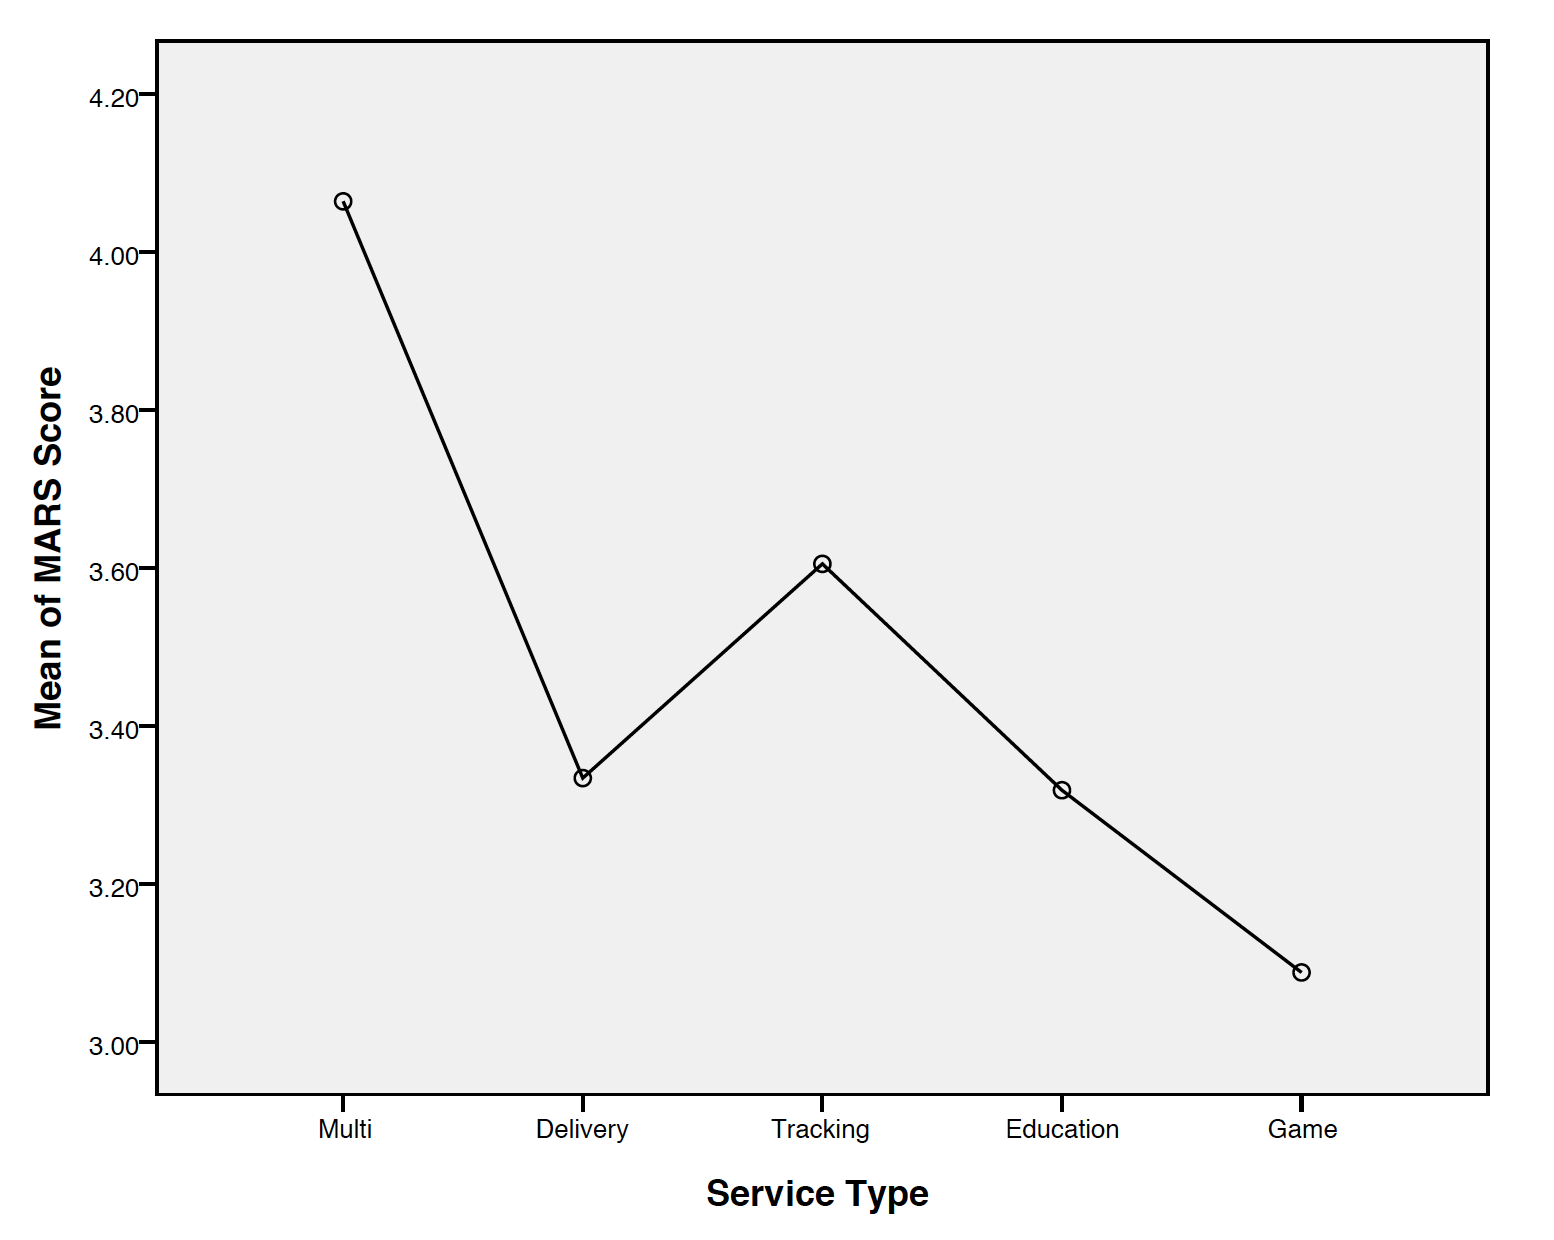
\includegraphics[scale=0.40, angle=0]{Files/prevention-study-1/figures/servicetype-mars-anova}
    \caption{Mean plot showing MARS score for Service Types}
    \label{fig: servicetype-mars-anova}
\end{figure}

\subsection{Education Format}
Apps were analysed to determine if they contained educational information, and if so, in which formats (i.e. text, image, audio, video, graphs, and human coaching).
Comparing apps which had an education component, with those that had not, using an independent samples t-test showed no significant difference in overall MARS score. There was however, a significant difference found in the information sub-scores for educational (M = 3.23, SD = .904 ) and non-educational apps (M = 2.82, SD = .916) at the p\textless.05 level [t(85) = -2.00, p = 0.048].
Further analysis of apps which contain educational information (n=56), showed that over 75\% used text as a method to provide educational information. Further details of formats and their frequencies can be seen in Table \ref{tbl: educationformat-frequencies}.

\begin{table}[h]
\centering
\caption{Frequencies of information format within apps that provided educational material}
\label{tbl: educationformat-frequencies}
\begin{tabular}{@{}lll@{}}
\toprule
Education Format & Frequency & Percentage \\ \midrule
Text & 44 & 78.6\% \\
Image & 13 & 23.2\% \\
Audio & 18 & 32.1\% \\
Video & 11 & 19.6\% \\
Graph & 2 & 3.6\% \\
Coach & 3 & 5.6\% \\ \bottomrule
\end{tabular}
\end{table}

An independent samples t-Test was conducted to compare MARS scores (including criteria sub-scores) in apps using text and no text. There was a significant difference in the MARS scores for apps using text (M = 3.63, SD = .579) or no text (M = 3.30, SD = .556) as an educational format [t(85) = -2.73, p = 0.08]. A similar result was found in apps using images and no images. There was a significant difference in the MARS scores for apps using images (M = 3.95, SD = .315) or no images (M = 3.38, SD = .585) as an educational format [t(85) = -3.58, p = 0.001]. No significant difference in MARS score was found in apps using or not using audio, video, graphs or human coaches.

These results suggest that textual information has an effect on the overall MARS rating. Specifically, the results suggest that using text to deliver educational information has a positive effect on the perceived efficacy of the app for the purposes of improving health.

\subsection{Tracking Methods}
Apps were analysed to establish if they facilitated tracking health metrics or behaviours, and if so, how this was performed. Forms of tracking were categorised as:
\begin{enumerate}[noitemsep,topsep=0pt]
\item \textbf{manual} self-tracking.
\item \textbf{automatic} tracking via smartphone sensors (e.g. step counter app).
\item structured program \textbf{progression}.
\item tracking via \textbf{connected} devices (e.g. wrist-worn activity monitors).
\end{enumerate}

52.0\% (n=46) of the apps reviewed facilitated some form of behavioural or health tracking. Frequencies of the tracking methods used within these apps can be seen in Table \ref{tbl: trackingtype-frequencies}. The majority of apps facilitate manual self-reporting. A potential reason for this is that whilst onboard sensors and connected wearables may detect and quantify physical activity and vital signs, self-reporting is the only method from which to extract qualitative measures, including perceptions of mood and stress.

\begin{table}[h]
\centering
\caption{Frequencies of tracking methods within apps that provided educational material}
\label{tbl: trackingtype-frequencies}
\begin{tabular}{@{}lll@{}}
\toprule
Tracking Method & Frequency & Percentage \\ \midrule
Manual & 34 & 73.9\% \\
Automatic & 3 & 6.5\% \\
Progression & 4 & 8.7\% \\
Connected & 4 & 8.7\% \\ \bottomrule
\end{tabular}
\end{table}

89.1\% (n=41) of the apps that facilitate tracking do so using only one method. An independent samples t-Test was conducted to compare MARS scores (including criteria sub-scores) in apps that facilitated tracking and those that did not. There was a significant difference in the MARS scores for apps that facilitated tracking (M = 3.73, SD = .464) and apps that did not (M = 3.17, SD = .579) [t(85) = -4.96, p = \textless0.00].
Statistical significance was also found within tracking/no tracking comparisons for the Engagement, Aesthetics and Subjective sub-criteria.
\newline There was a significant difference in the \textit{engagement} scores for apps that facilitated tracking (M = 3.57, SD = .711) and apps that did not (M = 2.54, SD = .768) [t(85) = -6.48, p = \textless0.00]. Significance in \textit{aesthetics} scores for apps that facilitated tracking (M = 4.07, SD = .755) and apps that did not (M = 3.30, SD = .726) [t(85) = -4.89, p = \textless0.00] and \textit{subjective} scores for apps that facilitated tracking (M = 3.28, SD = .954) and apps that did not (M = 2.01, SD = .626) [t(78.4) = -7.42, p = \textless0.00]. No significant difference was found in the functionality and information criteria scores.
A number of apps utilised more than one tracking method, as such, the quantity of tracking methods utilised by each app and tested for correlation with MARS scores. In apps that facilitated tracking (n=45), the quantity of tracking methods utilised showed no correlation with the MARS score (r = .056, p = .716).
%Number of tracking types facilitated

These results suggest that facilitating the tracking of behaviours has a significant effect on the overall MARS rating score, which is directly affected by engagement and aesthetic criteria scores. After the inclusion of any tracking method, the quantity of tracking methods does not influence score.

\subsection{Structured Progression}
%Examine if structured determines score?
Apps were analysed to establish if they provided a structured progression program, helping to guide users through various states or stages of the apps activity. For example, increasing physical activity goal values once previous goals are met, controlling exposure to difficult goals, or simply providing increasingly detailed information on a specific topic as the user becomes better informed. 32.2\% (n=28) of the apps were categorised as enabling structured progression.
An independent samples t-Test was conducted to compare MARS scores (including criteria sub-scores) in apps that were structured and not structured. There was a significant difference in the MARS scores for apps were structured (M = 3.80, SD = .458) and not structured (M = 3.31, SD = .581) [t(85) = -3.90, p = \textless0.00]. Statistical significance between structured and not structured apps was also found within the Engagement, Aesthetics, Information and Subjective sub-criteria scores.
\newline Significance in \textit{engagement} scores that were structured (M = 3.58, SD = .925) and not structured (M = 2.84, SD = .784) [t(85) = -3.87, p = \textless0.00].
\newline Significance in \textit{aesthetics} scores that were structured (M = 4.16, SD = .728) and not structured (M = 3.49, SD = .797) [t(85) = -3.75, p = \textless0.00].
\newline Significance in \textit{information} scores that were structured (M = 3.39, SD = .615) and not structured (M = 2.94, SD = 1.01) [t(79.67) = -2.60, p = \textless0.00].
\newline Significance in \textit{subjective} scores that were structured (M = 3.28, SD = 1.15) and not structured (M = 2.39, SD = .837) [t(40.8) = -3.6, p = 0.01]. No significant difference was found in the functionality criteria.

These results suggest that including a form of structured progression within the app has a significantly positive effect on the overall MARS rating, including ratings of engagement, aesthetics, and information.

\subsection{Gamification Methods}
Apps were analysed to establish if they contained elements of gamification, which included points, goals, achievements, rankings, and social competition. 34.5\% (n=30) of apps analysed implemented elements of gamification, with over 50\% (n=16) of these apps using more than 1 gamification element.
The most common gamification elements used were points, achievements and targets as seen in Table \ref{tbl: gamification-frequency}.

\begin{table}[h]
\centering
\caption{Frequencies of gamification elements within apps that implemented gamification}
\label{tbl: gamification-frequency}
\begin{tabular}{@{}lll@{}}
\toprule
Element & Frequency & Percentage \\ \midrule
Points               & 17        & 56.7\%     \\
Targets              & 16        & 53.3\%     \\
Achievements         & 15        & 50\%       \\
Rankings             & 6         & 20\%       \\
Social               & 4         & 13.3\%          \\ \bottomrule
\end{tabular}
\end{table}

Apps were analysed to establish if they provided a structured progression program, helping to guide users through various states or stages of the apps activity. For example, increasing physical activity goal values once previous goals are met, controlling exposure to difficult goals, or simply providing increasingly detailed information on a specific topic as the user becomes better informed. 32.2\% (n=28) of the apps were categorised as enabling structured progression.
An independent samples t-Test was conducted to compare MARS scores (including criteria sub-scores) in apps that had elements of gamification and no gamification. There was a significant difference in the MARS scores for gamification apps (M = 3.85, SD = .468) and no gamification app (M = 3.27, SD = .545) [t(85) = -5.018, p = \textless0.00]. Statistical significance between apps who implemented gamification, and those that did not, was also found within the Engagement, Aesthetics, and Subjective sub-criteria scores.
Significance in \textit{engagement} scores for gamification apps (M = 3.79, SD = .626) and no gamification app (M = 2.71, SD = .788) [t(85) = -6.50, p = \textless0.00]. Significance in \textit{aesthetics} scores for gamification apps (M = 4.29, SD = .628) and no gamification app (M = 3.40, SD = .765) [t(85) = -5.45, p = \textless0.00]. Significance in \textit{subjective} for gamification apps (M = 3.57, SD = .895) and no gamification app (M = 2.21, SD = .756) [t(85) = -7.47, p = \textless0.00]. No significant difference was found in the functionality or information criteria.

These results suggest that including gamification within the app has a significantly positive effect on the overall MARS rating, including ratings of engagement, aesthetics, and subjectivity.

The gamification elements were then examined to determine if the use of certain elements had an effect on the MARS score. An independent samples t-Test of apps that used at least one gamification element (n=30) showed a significant difference in MARS scores for apps that used achievements (M = 4.06, SD = .316), and those that did not (M = 3.65, SD = .511) [t(28) = -2.68, p = 0.12]. Although not statistically significant, there was a notable difference in engagement scores between apps that used points (M = 3.97, SD = .628), and those that did not (M = 3.56, SD = .569) [t(28) = -1.8, p = 0.08]. The remaining gamification types displayed no significant differences within independent samples t-Tests.

%Examine if gamification method determines score?
%Game methods vs each other
%Gamification vs rest

Correlation analysis showed that the number of gamification elements used and MARS score were significantly positively correlated at the p\textless.05 level (r = .518, p = \textless0.00). Linear regression analysis shows that the number of domains targeted explain a significant amount of the variance in the MARS scores [F(1, 85) = 22.5, p = \textless0.00, R\textsuperscript{2} = .210, R\textsuperscript{2}\textsubscript{Adjusted} = .200]. For every additional gamification element used, MARS score increased on average by 0.235. The linear regression line can be seen in Figure \ref{fig: gamification-regression} and the equation is as follows:

\begin{equation}
MARSscore = 3.316 + 0.235 \left(NumberGamificationElements\right)
          \label{eq: calc-performance-stars}
\end{equation}

\begin{figure}[h]
    \centering
    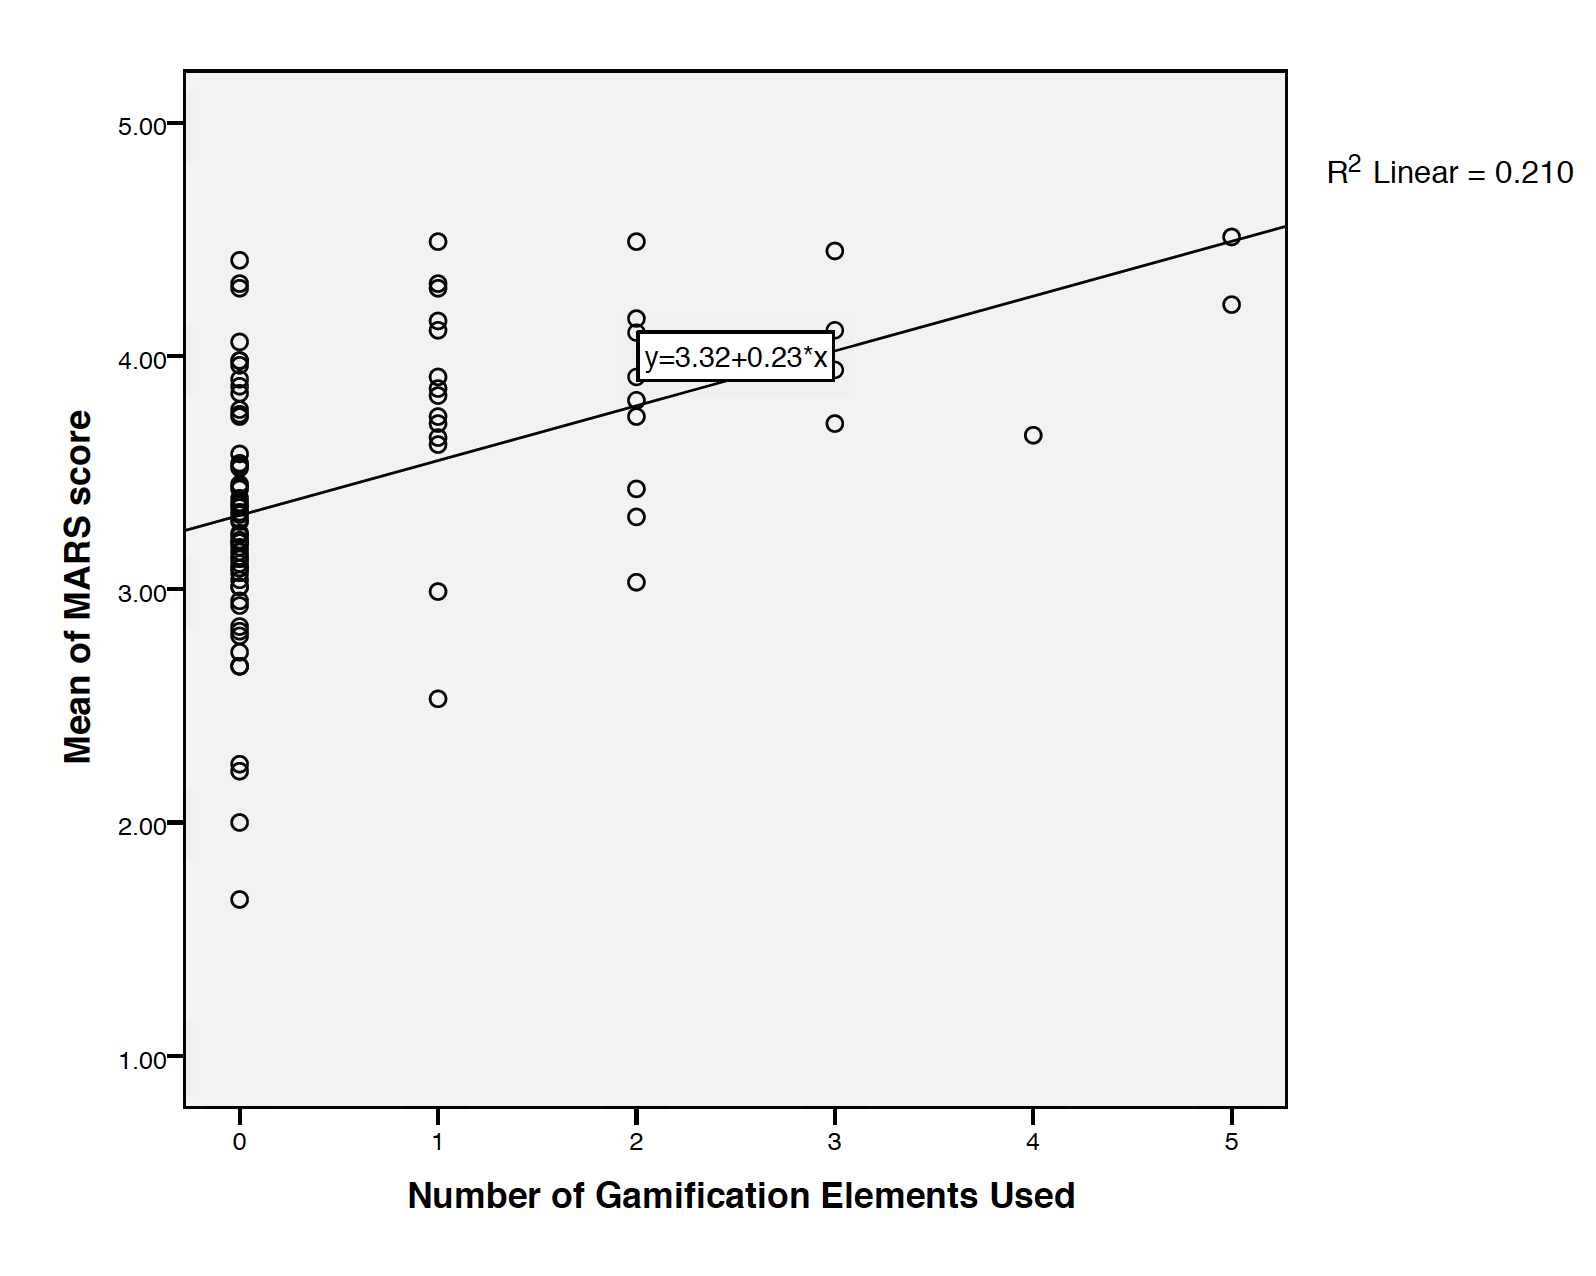
\includegraphics[scale=0.40, angle=0]{Files/prevention-study-1/figures/gamification-regression}
    \caption{Scatter plot showing MARS score against Number of Gamification elements used}
    \label{fig: gamification-regression}
\end{figure}

\subsection{Social Integration} \label{subsection: social-integration}
Each app was analysed to determine if it integrated any form of social media or networking. Examples of social integration include the creation of a friend network, sharing gamification points with friends, sharing progression with existing social networking contacts, comparison of results with friends. 23\% (n=20) apps implemented social elements into the app, the remaining 73\% (n=67) did not. An independent samples t-Test was conducted to compare MARS scores (including criteria sub-scores) in apps that integrated social elements and those that did not. There was a significant difference in the MARS scores for social apps (M = 3.83, SD = .457) and not social (M = 3.36, SD = .584) [t(85) = -3.73, p = 0.002]. Statistical significance was also found within the Engagement, Aesthetics, and Subjective criteria scores.
Significance at the p \textless 0.05 level was found between \textit{engagement} scores for social apps (M = 3.83, SD = .713) and non-social apps (M = 2.86, SD = .828) [t(85) = -4.70, p = \textless0.00]. Significance at the p \textless 0.05 level was found between \textit{aesthetics} scores for social apps (M = 4.21, SD = .686) and non-social apps (M = 3.56, SD = .818) [t(85) = -3.246, p = 0.002]. Significance at the p \textless 0.05 level was found between \textit{subjective} for social apps (M = 3.50, SD = .833) and non-social apps (M = 2.43, SD = .961) [t(85) = -4.49, p = \textless0.00]. No significant difference was found in the functionality or information criteria.

Results would suggest that integrating social elements within an app will positively affect the overall MARS score, including engagement, aesthetics, and subjective criteria scores.

\subsection{Media Use and Format}
In a similar fashion to how the analysis of education format was performed, each app was also analysed for the use of various forms of media, including audio, video, image, graphs, and games. 78\% (n=68) of the apps used some form of media to represent or deliver content to the user. The frequencies of each format can be seen in Table \ref{tbl: mediaformat-frequencies}. Excluding apps with no media, 72.1\% (n=49) of the media apps used only one format, 17.6\% (n=12) used 2, and 10.3\% (n=7) used 3 or more.  Correlation analysis showed that the number of formats used and the MARS score were significantly positively correlated at the p\textless.05 level (r = .309, p = 0.01).

\begin{table}[h]
\centering
\caption{Frequencies of media types used format within apps that used media}
\label{tbl: mediaformat-frequencies}
\begin{tabular}{@{}lll@{}}
\toprule
Media Format & Frequency & Percentage \\ \midrule
Image & 32 & 47.1\% \\
Audio & 31 & 45.6\% \\
Video & 13 & 19.1\% \\
Graph & 14 & 20.6\% \\
Games & 8 & 11.8\% \\ \bottomrule
\end{tabular}
\end{table}

Using an independent samples t-Test no significance was found in MARS score, or criteria sub-scores, between the use of media and not. There was, however, significance found in various sub-scores and the use of certain media formats. There was a significant difference found in subjective scores in the use of audio (M = 2.86, SD = 1.02), and not (M = 2.35, SD = .970) [t(85) = 2.253, p = 0.027].
There was a significant difference found through the use of images, and not, in the \textit{aesthetics} score (No Image = 3.50, SD = .815,  Image: M = 4.06, SD = .754) [t(85) = -3.14, p = 0.002], the \textit{engagement} score (No image: M = 2.93, SD = .835, Image: M = 3.36, SD = .945) [t(85) = -2.23, p = 0.028], and overall \textit{MARS} score (No image: M = 3.37, SD = .630, Image: M = 3.64, SD = .470) [t(85) = -2.14, p = 0.035].
There was also a significant difference found in the use of graphs, and not, in the \textit{aesthetics} score (No graph: M = 3.62, SD = .832, Graph: M = 4.17, SD = .470) [t(85) = -2.34, p = 0.021], and in the \textit{subjective} score (No graph: M = 2.51, SD = .986, Graph: M = 3.57, SD = .805) [t(85) = -3.77, p = \textless0.00].
In addition, a signifiant difference in \textit{engagement} scores were found in apps who used games (M =  3.02, SD = .86), and those that did not (M = 3.75, SD = 1.04) [t(85) = -2.24, p = 0.28].

These results indicate that the addition of specific visual formats, i.e. Images, Graphs and Games can increase sub-criteria scores. Conversely, the inclusion of auditory formats can decrease ratings in the subjective criteria. Note however, that the subjective is not taken into consideration when calculating the MARS score, so the importance is somewhat debatable.

\subsection{Condition Focus}
Of the 87 apps, 12 (13.8\%) apps focus on a specific health condition, with the remaining 75 (86.2\%) stating to improve health in a general sense. Of the condition focused apps (n=12), conditions targeted are Alzheimer's disease (n=4, 33\%), Depression (n=2, 16.7\%), Insomnia (n=2, 16.7\%), Post Traumatic Stress Disorder (PTSD) (n=1, 8.3\%), Anorexia (n=1, 8.3\%), Suicide Prevention (n=1, 8.3\%), and Controlling Blood Pressure (n=1, 8.3\%). An independent samples t-Test was conducted to compare MARS scores (including criteria sub-scores) in apps that focused on a health condition and those that did not. There was no significant difference found between the groups at the p \textless 0.05 level.
One-way ANOVA was used to compare the effect of the condition focus type on the MARS score. ANOVA analysis showed there was no significant difference between the groups. Further analysis was then performed, removing groups which had fewer than 2 cases. The remaining apps were specifically focused on Alzheimer's Disease (n = 4, M = 3.36), Depression (n = 2, M = 2.95), and Insomnia (n = 2, M = 2.93). No significant difference was found between the groups in MARS scores or any criteria sub-scores.

\subsection{Pricing}
Each app's price was categorised based upon it's cost to the user. Apps were categorised as Free (61.8\%), Paid (8.8\%), Subscription (4.4\%), and In-App (25\%). Free apps do not incur any cost to download or use. Paid apps are those that incur a one-time fee to download the app, after which it belongs to the user. Subscription apps are free to download, but are based upon a service delivery model, whereby the user pays to use the app on a time or service based quota. The In-App category describes apps that are free to download, but have additional content that can be purchased to supplement or expand upon the originally free material.
One-way ANOVA was used to compare the effect of the pricing type on the MARS score. ANOVA analysis showed there was a significant effect of pricing type on the MARS Score at the p\textless.05 level [F(3, 83) = 4.521, p = 0.05]. Post hoc comparisons using the Bonferroni test indicated that the mean score for Subscription type apps (M = 4.20, SD = 0.214) was significantly different than Free (M = 3.39, SD = 0.60, p=0.016) and Paid apps (M = 3.14, SD = 0.478, p=0.010). This can be seen in Figure \ref{fig: pricetype-mars-anova}. An independent samples t-Test between apps that use the subscription pricing model, and those that do not, highlighted that a significantly larger proportion of subscription apps implemented structured progression (M = .80, SD = .447), than other pricing types (M = .29, SD = .458) [t(85) = -2.40, p = 0.18]. As with previous analysis, the inclusion of structured progression is associated with increased MARS scores.

Further analysis was performed between apps that used the subscription model (n=5), and those that did not (n=82). A Pearson's Chi-Square test was performed which showed that the subscription model was significantly related to the use of structured progression (x\textsuperscript{2}(1) = 5.557, p = 0.018, Cramer's V = .253). Only 29.3\% of other pricing types implemented structured progression, whilst 80\% of subscription apps implemented structured progression, which has been previously shown to positively affect the MARS score.

\begin{figure}[h]
    \centering
    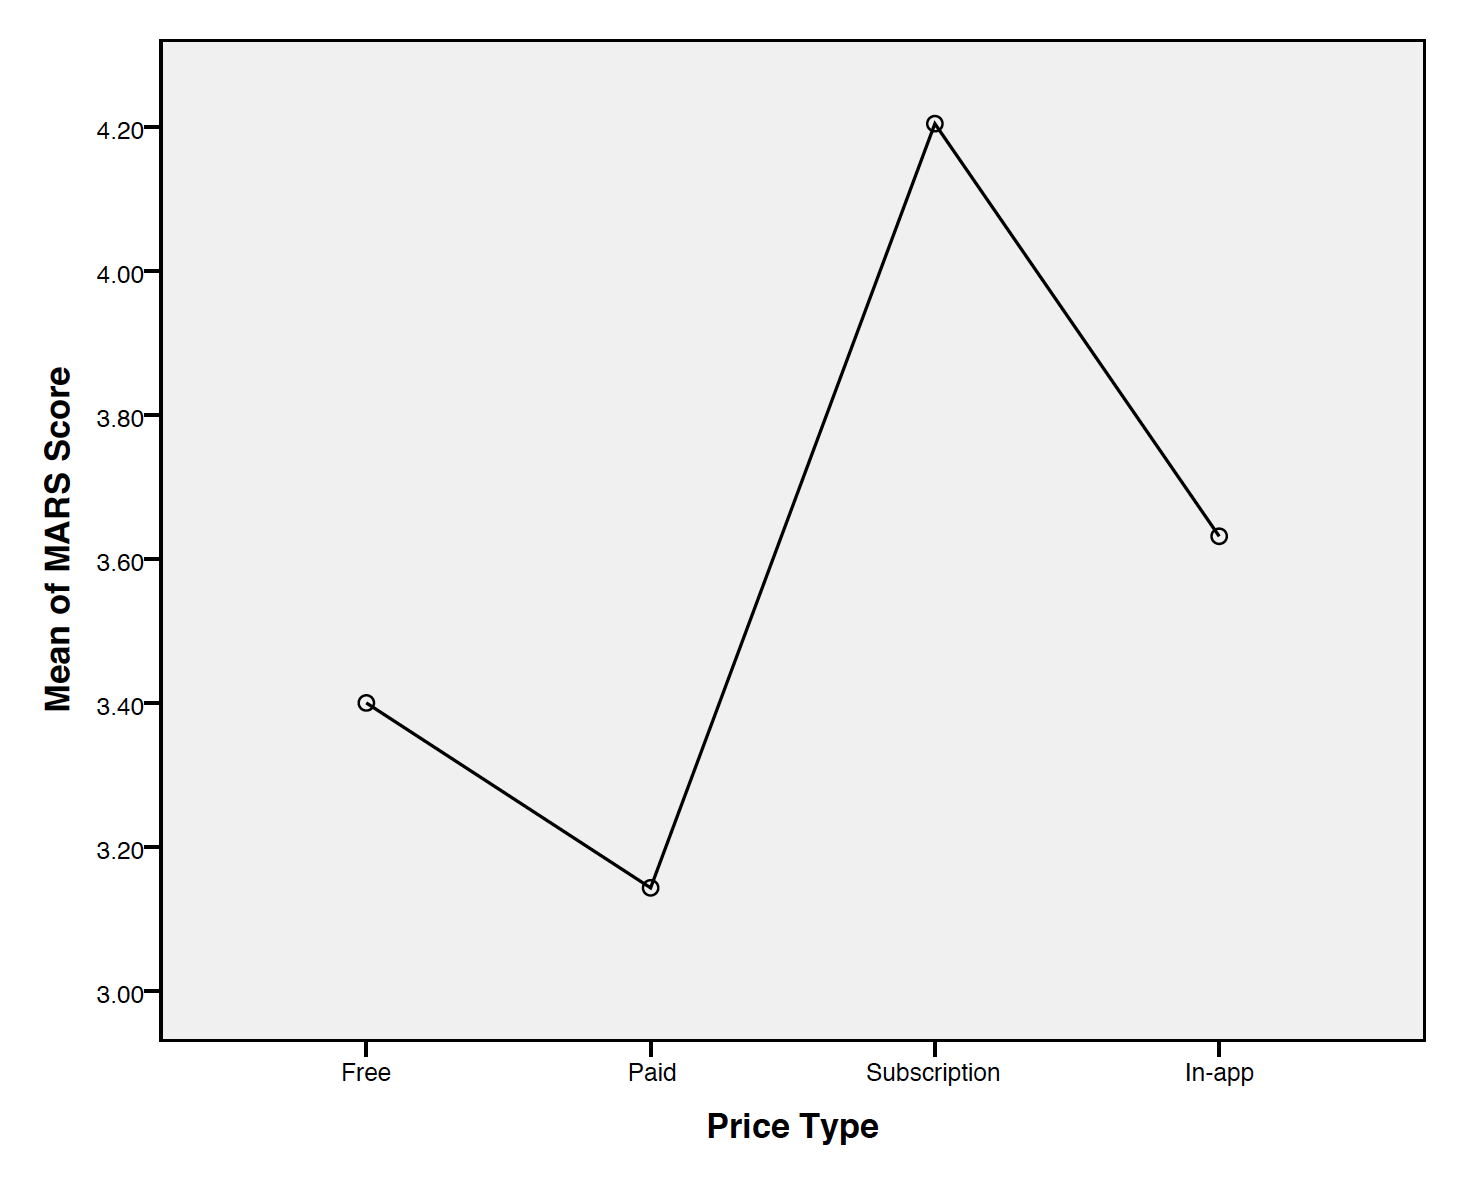
\includegraphics[scale=0.40, angle=0]{Files/prevention-study-1/figures/pricetype-mars-anova}
    \caption{Mean plot showing MARS score for Price types}
    \label{fig: pricetype-mars-anova}
\end{figure}

\subsection{Discussion} \label{subsection: MARS-discussion}
From analysing the elements within each app, a number of important observations were made. The inclusion of certain elements had a significantly positive effect on the overall MARS score, often influenced by significant impact in criteria sub-scores. The following summarises the observations:

\begin{enumerate}[noitemsep,topsep=0pt]
\item Targeting \textbf{multiple domains} results in a significantly higher MARS score.
\item Providing \textbf{more than one primary service} results in a significantly higher MARS score.
\item Providing \textbf{educational information} significantly increases information scores.
\item Inclusion of \textbf{text as an education format} significantly increases MARS score in all apps.
\item The \textbf{use of images} to supplement education material significantly increases MARS scores.
\item \textbf{Facilitating tracking} significantly increases engagement, aesthetics, subjective and overall MARS scores.
\item There is \textbf{no relation} between score and quantity of tracking methods.
\item Apps which provide a \textbf{structured program} have a significantly higher MARS, engagement, aesthetics, information, and subjective criteria scores.
\item Apps which \textbf{utilise elements of gamification} have significantly higher MARS, engagement, aesthetics, and subjective criteria scores.
\item Use of the \textbf{achievements} gamification element results in a significantly higher MARS score.
\item The \textbf{number of gamification elements} used was significantly positively correlated with the MARS score.
\item The integration of \textbf{social elements} result in a significantly higher MARS score.
\item No significant difference was found in apps that used \textbf{media and no media}.
\item In apps that used media, significant differences were found between the \textbf{media formats used}, with the highest scores resulting from the use of images, graphs and games.
\item The \textbf{number of media formats} used was significantly positively correlated with the MARS score.
\item No significant difference was found in any scoring metric within apps that \textbf{targeted a specific health condition}and those that did not.
\item Free apps were rated higher on average than one-off payment apps, but lower than subscription and in-app purchase apps.
\item Apps which use a \textbf{subscription based pricing model} have a significantly higher MARS score.
\end{enumerate}

From these results it is clear that a number of recommendations may be made for an app which aims to score highly on the MARS scale. Such recommendations include the utilisation of multiple services addressing multiple behavioural domains, clear information delivery provided through numerous media formats, with a specific focus on imagery, facilitating tracking, and the inclusion of gamification elements, specifically the use of points and achievements.

\subsubsection{The Gray Matters App}
The Gray Matters app incorporates many of the recommendations that have been uncovered through the content analysis in the previous section. The app targets 7 domains, provides educational material, facilitates tracking, facilitates structured progression, and implements gamification through point scoring. However, the app does have a number of shortcomings; utilising only 1 form of education delivery (text), facilitating tracking through self-report only, and graphs are the only form of multimedia used.

\textbf{Regression Accuracy.} Using the regression equations from the number of domains targeted and number of gamification elements predicted that the MARS score would be 4.332, and 3.786 respectively.
Both scores underestimated the true score attributed by the expert reviewers of 4.53. This score however, is the result of only 5 expert reviewers, heavily skewed by the 4:1 Medicine:Computer Science ratio. Further research and recruitment of experts from neighbouring domains is needed to ensure the rating is valid.

\section{Conclusion}
This chapter has presented the developed applications merit through expert review and contrast with existing apps, both in the commercial and research domain. Content analysis of 87 apps also uncovered valuable recommendations for the development of a successful mHealth app, and served to expose the current shortcomings of the Gray Matters app.
 % 5 GM Evaluation
\chap{Evaluating the Efficacy of a Novel Behaviour Change App with Intended Patient Population} \label{chapter: prevention-rctresults}

\setlength{\epigraphwidth}{.50\textwidth}
\begin{epigraphs}
\qitem{It remains an ideal that all new healthcare interventions should be evaluated through randomised controlled trials.}
{--- \textsc{Prof. Bonnie Sibbald} \\ \textit{Former Chair of the UK Health Services Research Network}}
\end{epigraphs}

This Chapter details the results from a 6-month RCT which aimed to reduce participant's AD risk in later life, using the developed Gray Matters app.

\section{Introduction}
To truly evaluate the mobile behaviour change intervention framework, it must be used within its intended environment, and with its intended user population. With the framework applied to the application area of AD, the Gray Matters app was created, and subsequently evaluated from a technology viewpoint, by expert raters in the domain area. The final test of efficacy is assessing the apps use as a tool to change behaviour with an appropriate study cohort. As such an RCT was designed to evaluate the app over 6-months with a cohort of 144 persons\footnote{ClinicalTrials.gov Identifier: NCT02290912}. This study was performed in collaboration with researchers from the Department of Psychology and the Department of Family, Consumer, and Human Development at Utah State University \cite{Norton2015-TRCI}. 
%VIVA: Chris -In my opinion this is the main contribution to knowledge that your Thesis makes

\section{Study Design}
The study was an RCT; delivered over a 6-month period, commencing in April 2014, with post-test collection performed at the close.
The study was designed as an intervention, and consisted of subjects who were randomly assigned into either treatment or control groups. Those assigned to the treatment group were given access to the Gray Matters app and additional intervention components. The treatment group were not given a strict regimen and therefore a wide range of engagement levels were anticipated. The control group were not given access to any intervention components and were used for baseline comparisons. A uniform random number generator (0,1) within SPSS v21 was used to randomise participants into treatment and control groups, with the aim of allocating 1/3 of the participants to control, and 2/3 to treatment.

\subsection{Recruitment}
Recruitment of participants was achieved by emailing announcements to faculty, alumni and staff of Utah State University and distributing flyers at health fairs and other venues, assisted by the local health department and their community liaisons. For those interested a pre-screening eligibility survey was completed. Eligibility criteria included:
\begin{enumerate}[noitemsep,topsep=0pt,label=(\alph*)]
\item Age between 40 and 64 years.
\item BMI no greater than 41.
\item Possession of a smartphone or tablet (iOS or Android only)
\item Fluency in the English language
\item Residence in Cache County, Utah, United States of America.
\item Not having any of the following medical conditions: pregnancy, dementia, unmanaged diabetes, or untreated major depression.
\end{enumerate}

\subsection{Statistical Power}
To achieve 80\% statistical power to detect a medium effect size (Cohen's d=.50) when comparing the difference between two independent means at a 2:1 (treatment:control) ratio, 96 treatment and 48 control (144 total) participants were needed, calculated using G*Power \cite{Faul2007}. Upon randomisation participants were allocated to each group, however, to avoid intra-couple contamination of intervention material, married couples were assigned to the same randomised group (n=12). This adjustment resulted in 104 participants assigned to treatment and 42 to control, resulting in an approximate 5:2 ratio (treatment:control).

\subsection{Outcome Measures}
Outcome measures for the RCT study were categorised as primary, secondary, and tertiary outcome measures.
\newline Primary outcome measures included a set of anthropometric measures and blood-based biomarkers that are associated with AD onset in the literature. All measures are continuous variables, however, they have been categorised into categorical variables where appropriate, as shown in Table \ref{tbl: clinical-variables}.
\newline Secondary outcome measures included behavioural measures conducted through a battery of tests to assess metacognition, motivation, readiness-for-change, sleep quality, social engagement, depression, and couple satisfaction (among married persons), and are detailed in Table \ref{tbl: behavioural-variables}.
\newline Tertiary outcome measures included app statistics derived from analytical code, including time spent using app, number of launches per week, and usage patterns. Demographic variables were also recorded, examples include gender, ethnicity, marital status and house hold income and are detailed in Table \ref{tbl: demographic-variables}.
\newline Tables containing full summaries of all recorded values at the beginning of the study, for all 146 Gray Matters study participants, are detailed by \citeauthor{Norton2015-TRCI} in \cite{Norton2015-TRCI}.

\begin{table}[h]
\centering
\caption{Clinical and laboratory biomarkers recorded for each participant.}
\label{tbl: clinical-variables}
\begin{tabular}{@{}ll@{}}
\toprule
Measures & Categorical (where appropriate) \\ \midrule
Body Mass Index (kg/m\textsuperscript{2}) & \begin{tabular}[c]{@{}l@{}}Underweight, Normal \\ Overweight, Obese (Class I-III)\end{tabular} \\
Systolic blood pressure (mmHg) & N/A \\
Diastolic blood pressure (mmHg) & Low, Ideal, Pre-High, High \\
Pulse (bpm) & N/A \\
C-reactive protein (mg/L) & N/A \\
Glucose, serum (mg/dL) & N/A \\
Insulin ($\mu$IU/mL) & N/A \\
HDL cholesterol (mg/dL) & Low, Medium, High \\
LDL cholesterol (mg/dL) & \begin{tabular}[c]{@{}l@{}}Optimal, Near Optimal \\ Borderline High, High, Very High\end{tabular} \\
Total cholesterol (mg/dL) & N/A \\
Triglycerides (mg/dL) & N/A \\ \bottomrule
\end{tabular}
\end{table}


\begin{table}[h]
\centering
\caption{Behavioural variables recorded for each participant based on self-rated physical, cognitive, social, emotional and nutritional health.}
\label{tbl: behavioural-variables}
\begin{tabular}{@{}ll@{}}
\toprule
Measure & Scale \\ \midrule
Overall physical health & 1-3 \\
Metacognition (memory now vs. 3 years ago) & 1-4 \\
Lifestyle Change Priority & \\
\textit{- Physical Activity} & 1-5 \\
\textit{- Healthy Food Choices} & 1-5 \\
\textit{- Stress Management} & 1-5 \\
\textit{- Cognitive Stimulation} & 1-5 \\
\textit{- Sleep Quality} & 1-5 \\
\textit{- Social Engagement} & 1-5 \\
NIH Toolbox SOCIAL &  \\
\textit{- Emotional Support} & 8 - 40 \\
\textit{- Friendship} & 8 - 40 \\
\textit{- Loneliness} & 5 - 25 \\
\textit{- Hostility} & 8 - 40 \\
Pittsburg Sleep Quality Index \cite{Buysse1989} & 0 - 21 \\
Perceived Stress Scale \cite{Cohen1983} & 0 - 56 \\
CES-D Depression scale \cite{Radloff1977} & 0 - 60 \\
Situational Motivational scale \cite{Guay2000} & 1 - 7 \\
R-URICA Readiness for change scale \cite{McConnaughy1983} & 0 - 10 \\
Couple Satisfaction Index \cite{Funk2007} & 0 - 160 \\
Dietary Approaches to Stop Hypertension (DASH) score \cite{Block1990} & 0 - 40 \\ \bottomrule
\end{tabular}
\end{table}

\begin{sidewaystable}
\centering
\caption{Demographic categorical variables recorded for each participant.}
\label{tbl: demographic-variables}
\resizebox{\textwidth}{!}{%
\begin{tabular}{@{}ll@{}}
\toprule
Variable                                                 & Categories                                                                                                                 \\ \midrule
Gender                                                   & Male / Female                                                                                                              \\
Race                                                     & White / Black or African American / Asian /  Native Hawaiian or Other Pacific Islander /American Indian / Other            \\
Marital status                                           & Married / Widowed / Divorced / Never Married                                                                               \\
Religious Affiliation                                    & Catholic or Protestant / LDS (Mormon) / Atheistic or Agnostic / Other (Jewish, Eastern, Other)                             \\
Education                                                & High School / College or Trade/ College B.S. or B.A. graduate/ Graduate or professional                                    \\
Income                                                   & \textless \$45k \$45-55k / \$55-75k / \textgreater \$75k                                                                                  \\
Family history of dementia                               & None/ Mother or Father/ Mother and Father/ Maternal GP or Paternal GP / Maternal GP and Paternal GP / Aunt, Uncle, Sibling \\
Dementia caregiving                                      & Never / Yes, but in past / Yes, currently                                                                                  \\
Smart device in treatment group  & iPhone / iPad /android phone / android tablet (Not mutually exclusive)                                                                              \\
Education                                                & High School / College or Trade/ College B.S. or B.A. graduate/ Graduate or professional                                    \\ \bottomrule
\end{tabular}}
\end{sidewaystable}

For the purposes of this Chapter, these outcome measures have been categorised into 3 overlapping categories, and are discussed later within the Chapter:
\begin{enumerate}[noitemsep,topsep=0pt]
	\item App Usage
	\item Behaviour Change
	\item Clinical Measures
\end{enumerate}

\subsection{Intervention Components}
In addition to the aforementioned Gray Matters smartphone app, participants in the treatment group also had access to a number of additional components to encourage engagement with the study. These included a wrist-worn activity monitor, booster-events, a personal coach and a study website.

\subsubsection{Smartphone App}
The Gray Matters app was used within the study, however, the method of distribution to the cohort was modified from that outlined in the framework in Chapter \ref{chapter: prevention-framework}. For the purpose of the clinical study, the decision was made to exercise additional control over the accessibility of the app. The app was not distributed via public app stores, however, rather by using a testing-platform named TestFlight\footnote{Since the study, Apple Inc. have purchased the company and it is accessible to Apple Developers only via \url{https://developer.apple.com/testflight/}}. In order for participants to download the application from TestFlight, they first needed to register an account with the service and request access to the app. This access request then had to be approved by the trial co-ordinators. These additional security steps did cause some issues for the participants during their on-boarding with the study. Nevertheless, the app was successfully downloaded and installed by all 104 participants in treatment, with weekly installations displayed in Figure \ref{fig: number-installs}.

\begin{figure}[h]
    \centering
    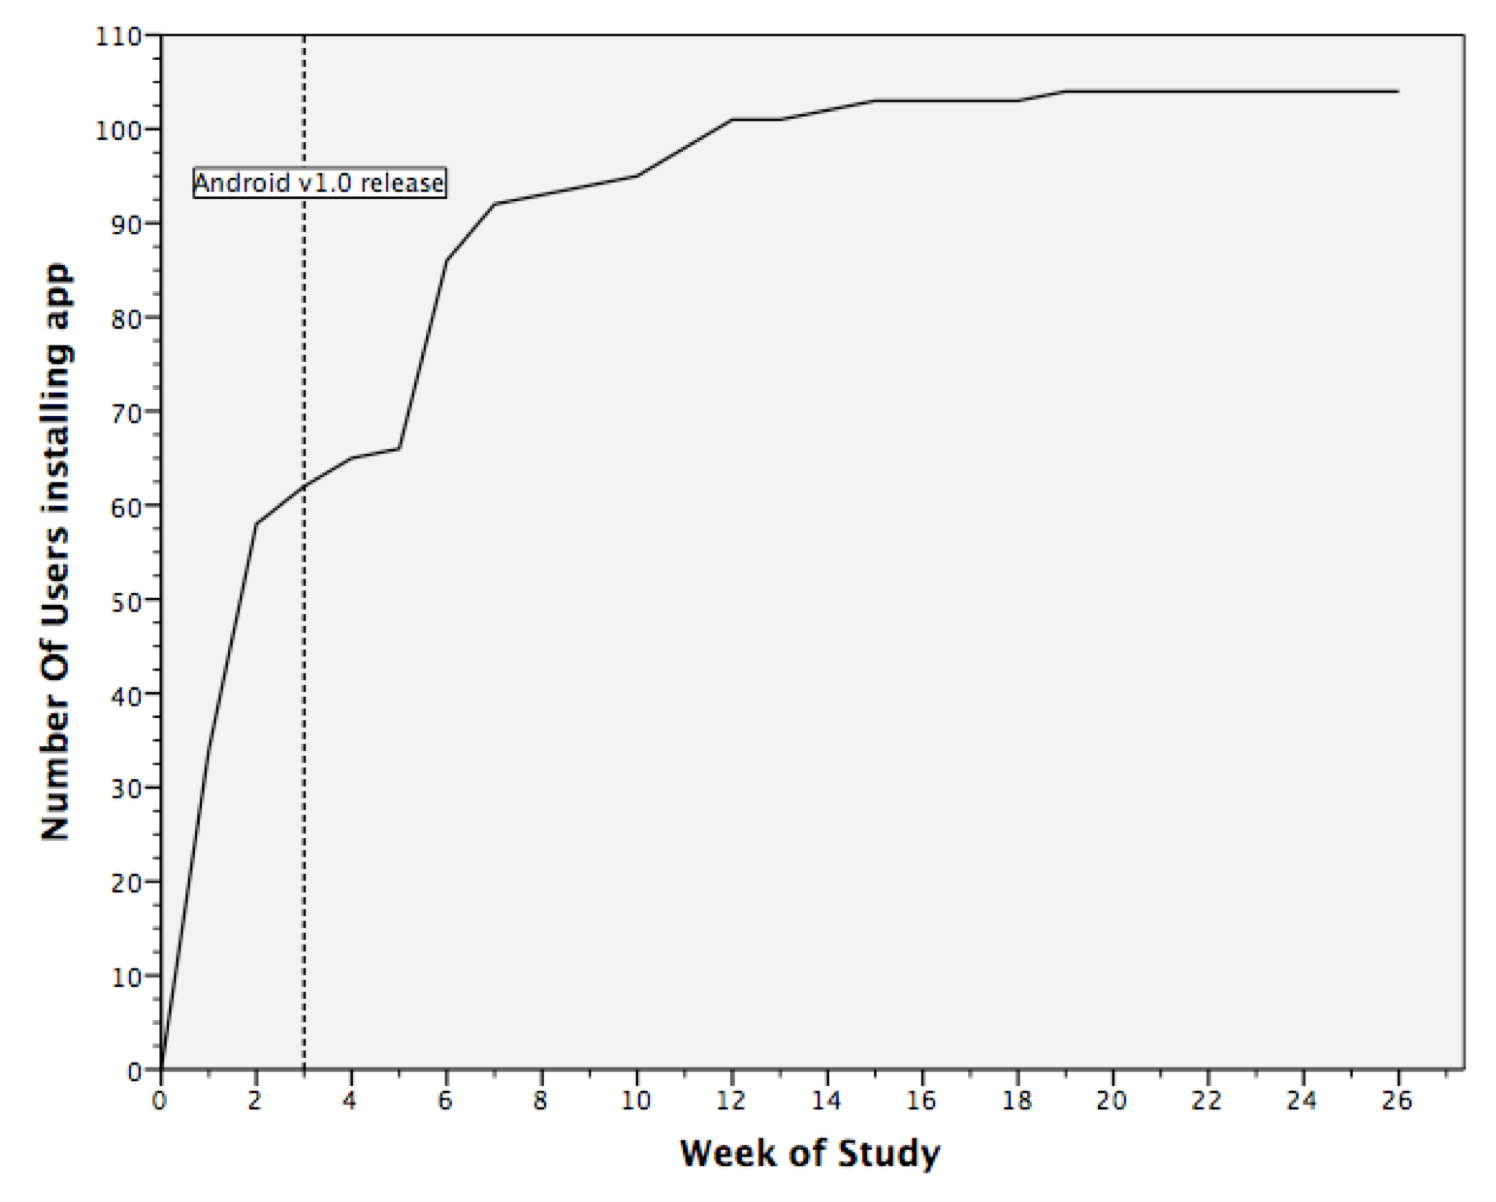
\includegraphics[scale=0.25, angle=0]{Files/prevention-study-3/figures/installs-by-week}
    \caption{Line graph showing cumulative installs by week.}
    \label{fig: number-installs}
\end{figure}

\subsubsection{Wearable Activity Monitor}
A wearable activity monitor was desired, both as a motivational factor, however, also as a means to validate self-reported behaviours. The Nike Corporation donated 150 Nike+ FuelBand SE activity monitors, hereafter referred to as FuelBands \footnote{For technical specifications refer to manual available online at \url{https://support-en-us.nikeplus.com/app/answers/detail/a_id/21032/p}}, for the purpose of the study. Each participant was given a FuelBand. This device is worn on the wrist and serves to collect information on physical activity performed throughout the day, such as steps taken, stairs climbed and total minutes of activity. This information is then consolidated into Nike's proprietary metric of ‘Fuel Points’. This device not only serves to collect data, it also acts as a physical reminder and motivator to increase levels of activity. Participants were asked to manually enter their total number of Fuel Points earned at the end of each day via the smartphone’s log tab.

\subsubsection{Booster Events}
All participants had the option of attending organised booster events. A booster event was designed to emphasise the link between specific actions of a behavioural domain, and the positive effect they had to minimising AD risk. This typically included examples of activities that could be applied in the participants daily routine. For example, a booster event that focused on the food domain hosted cooking classes that promoted sustainable healthy eating choices, whilst educating attendees about the link between the ingredients and AD risk. In total 46 booster events were organised and delivered across the 6-month intervention period. Attendance for each event is presented in Figure \ref{fig: booster-attendance}.

\begin{figure}[h]
    \centering
    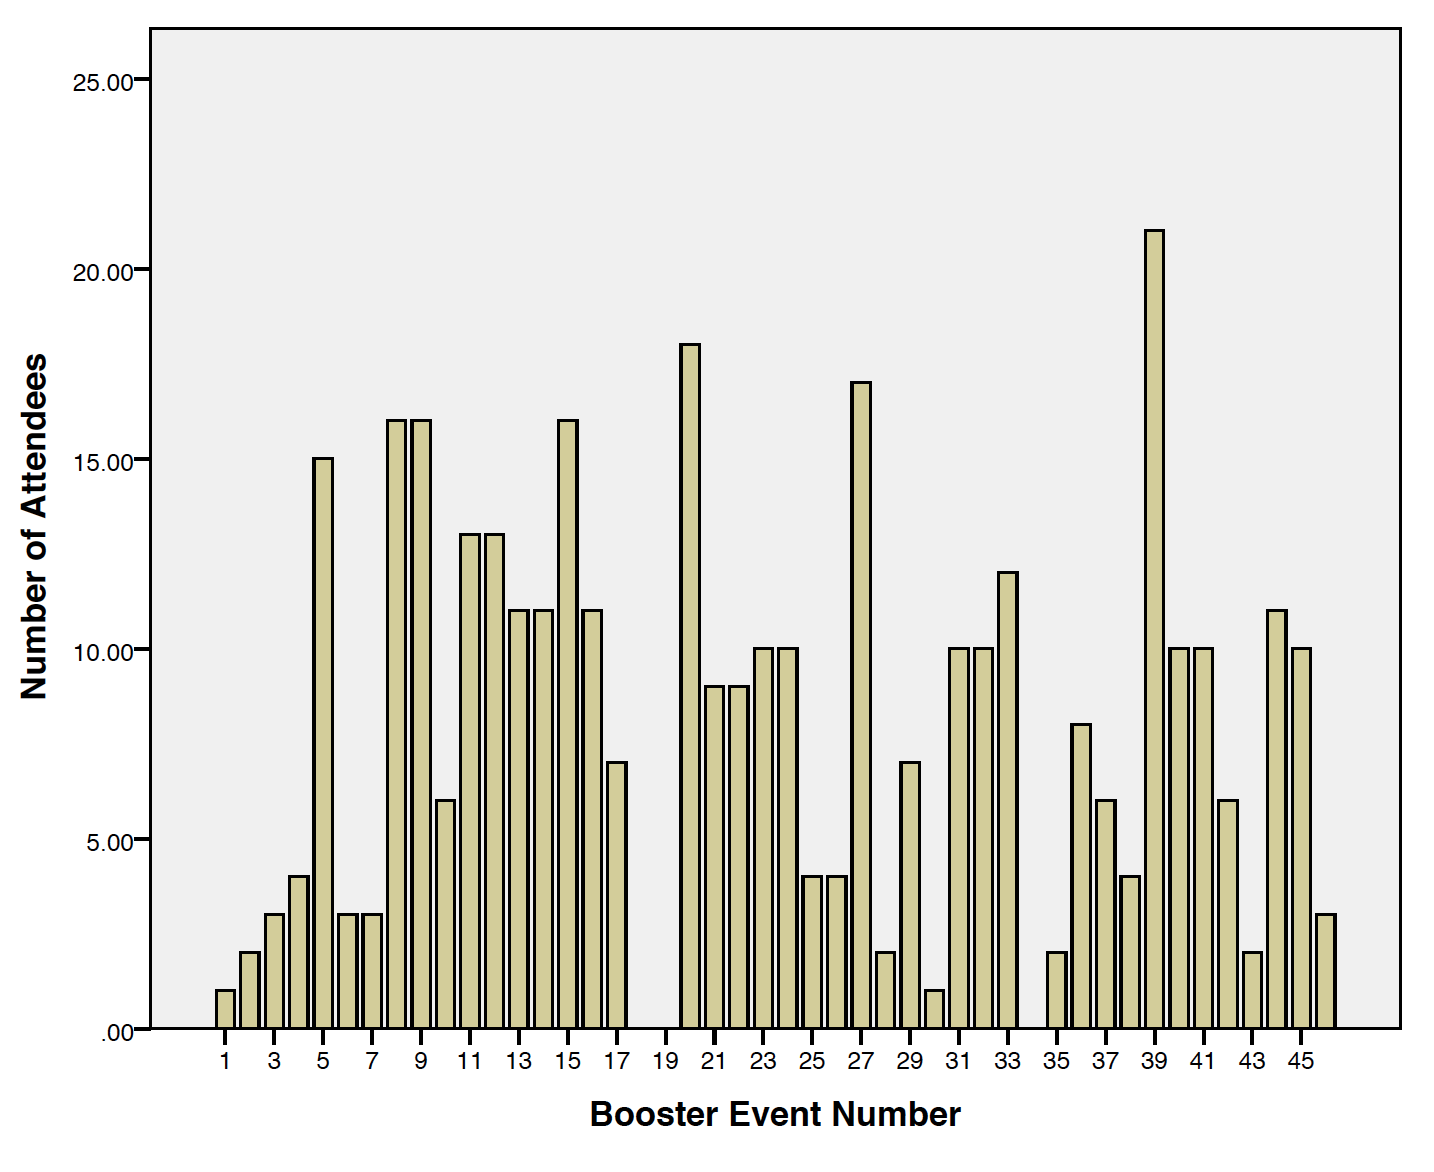
\includegraphics[scale=0.5, angle=0]{Files/prevention-study-3/figures/booster-attendance.png}
    \caption{Bar graph showing attendance numbers of each booster event.}
    \label{fig: booster-attendance}
\end{figure}
%VIVA: Can I colour code which event was which domain

As shown in Table \ref{tbl: booster-domain-freq}, the majority of booster events where focused on the Physical domain, followed by Food and Stress. The attendance figures, however, show the most popular domains with regards to attendance were Sleep and Cognitive.

\begin{table}[h]
\centering
\caption{Frequency statistics of domains targeted and attendance figures at booster events.}
\label{tbl: booster-domain-freq}
\begin{tabular}{@{}lllll@{}}
\toprule
Domain & Frequency & Percent & \begin{tabular}[c]{@{}l@{}}Attendance \\ (Mean)\end{tabular} & \begin{tabular}[c]{@{}l@{}}Attendance \\ (Std. Dev)\end{tabular} \\ \midrule
Physical & 15 & 32.6\% & 6 & 5.07 \\
Food & 9 & 19.6\% & 5.78 & 4.81 \\
Social & 2 & 4.3\% & 6.50 & 4.95 \\
Sleep & 4 & 8.7\% & 12 & 3.16 \\
Cognitive & 7 & 15.2\% & 12.14 & 6.14 \\
Stress & 9 & 19.6\% & 8.78 & 5.11 \\ \bottomrule
\end{tabular}
\end{table}
\subsubsection{Personal Coach}
Participants also had access to a personal coach with whom they could contact if they required assistance with any aspect of the behavioural domains. A team of 28 student interns with majors in the six behavioural domains volunteered to be personal coaches. Student coaches were trained in motivational interviewing and the transtheoretical model. Where needed, the coaches provided weekly email or text message exchanges with their assigned participants to provide emotional support and encouragement for lifestyle change goals. This component of the study was, however, vastly under-utilised, with many participants reporting at the study close that they did not know they had the facility \cite{Weyerman2015}.
% 11.11.15 - Emailed Maria regarding statistic on how many used the coach. No results yet.

\subsubsection{Study Website}
Participants also had access to a password protected website \cite{Norton2014} that provided supporting material to aid the use of the app and wearable device, which included instructional YouTube videos providing walkthroughs of the Gray Matters app for iOS and Android. In addition an email address was provided should additional issues arise.

\subsubsection{Exit Survey}
An exit survey was designed to capture opinions of participants in the treatment group. The survey asked questions about app usage, motivations, their perceived behaviour change and social network usage. At the end of the study 98\% (n=102) of the participants completed this survey.

\section{App Usage}
A mixture of open-source, and proprietary analytical tracking tools developed by the author were embedded into the runtime code of the apps. This allowed for numerous events, and in-app actions to be tracked over the period of the study. Using this data it was possible to determine levels of adoption, time spent using the app, behaviour patterns when self-reporting, and general patterns of app usage.

\subsection{Adoption}
In Week 1 (10th April 2014) the first iOS version of the app was released to the treatment group. This was performed through a launch event, in which attending participants were informed of the process of how to signup and download the application through the TestFlight platform. By the end of week 1, 31.7\% (n=33) participants had installed the app onto their iPhone and/or iPad. In week 3 (13th May 2014), the first Android version of the app was released to the treatment group due to demand from android users. Two weeks after this release, 19.2\% (n=20) participants had installed the first version of the Android app. By week 10, 86.5\% of the treatment group (n=90) had installed an iOS or Android version of the app onto their smartphone and/or tablet, with the remainder signing up shortly afterward, as seen in Figure \ref{fig: number-installs}. By week 12, over 100 participants had installed the app on their device. Many users opted to install the Gray Matters app on both their smartphone and tablet.
Of the 104 users using the app, at the end of the study, 75.97\% of all Gray Matters app sessions were on iOS devices (iPhone: 54.7\%; iPad: 21.27\%) and the remainder on Android devices (24.03\%).

\subsection{Duration of Use}
The average duration of each session with the app, across all devices, was 1 minute 55 seconds. This time is under the originally specified goal of 2 minutes for a user's session duration.

\subsection{Self-Reporting}
Over the duration of the study, over 122,719 behavioural logs were uploaded to the central database. The average user answered 7.3 $ \pm $ 3.16 questions per day during their participation in the study. To further understand the self-reporting process, additional analytical tracking code was added to the app in Week 18. This allowed the investigators to analyse specific behaviours when answering questions in the log screen. One function allowed investigators to quantify the number of times the user altered their behavioural values. Figure \ref{fig: bargraph-questionedits} presents the mean number of times each domain's questions were updated in the self-reporting screen.

 \begin{figure}[h]
    \centering
    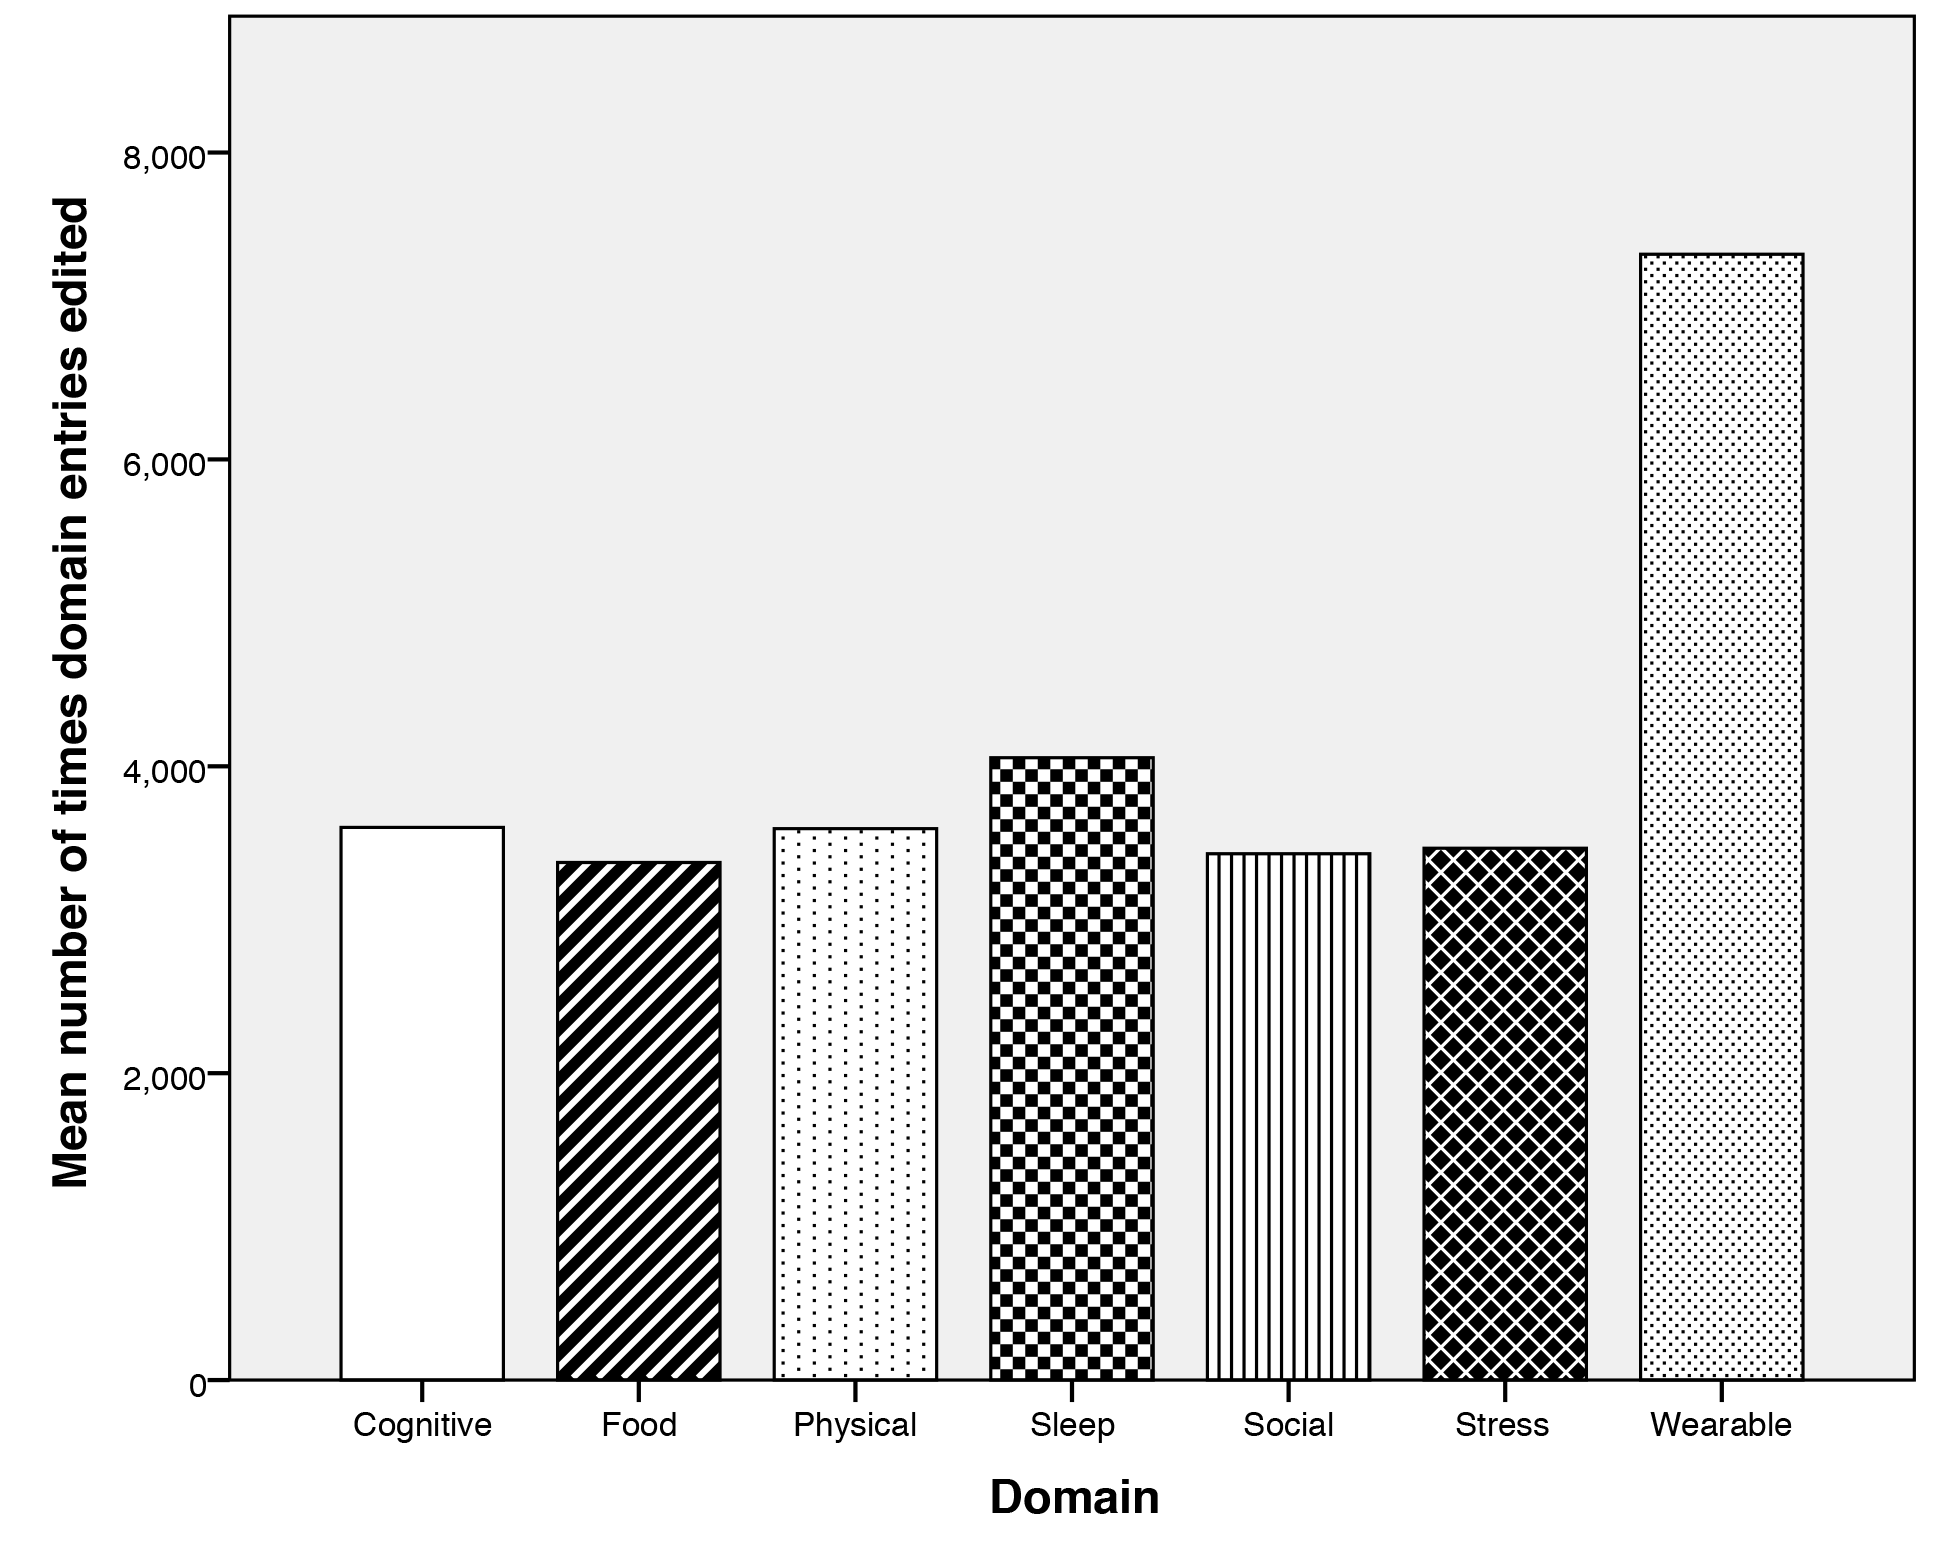
\includegraphics[scale=0.2, angle=0]{Files/prevention-study-3/figures/domain-edits}
    \caption{Bar graph showing the mean number of times each domain’s questions were edited using the sliders in the log screen, using updated analytical code, from week 18 to study end. The wearable domain is updated almost twice as often as the other domains.}
    \label{fig: bargraph-questionedits}
\end{figure}

Across all users in the study, Question 12 was altered a statistically significant amount more than the rest (z = 3.054, p = .0023). Question 12, belongs to the Wearable domain and relates to the number of Nike fuel points earned. It is assumed that users frequently updated this amount, more than the others, due to the variability in the data generated from the wearable device each day when they were active. This also indicates that integration with the wearable devices at a communications level would greatly reduce the need for participant interaction.

\subsection{Time of Day} \label{subsection: time-of-day}
Analytical tracking code also enabled the investigators to observe the patterns of usage with relation to time of day. Figure \ref{fig: time-of-day} shows that usage peaks at 2 points in the day, the first in a short period in the morning around 7-9am. In the evening, however, app usage rapidly increases around 8pm and declines sharply after 11pm. It is believed that the users wait until the end of the day before entering their log data, so that it is the most valid representation of their behaviours in that daily period.

 \begin{figure}[h]
    \centering
    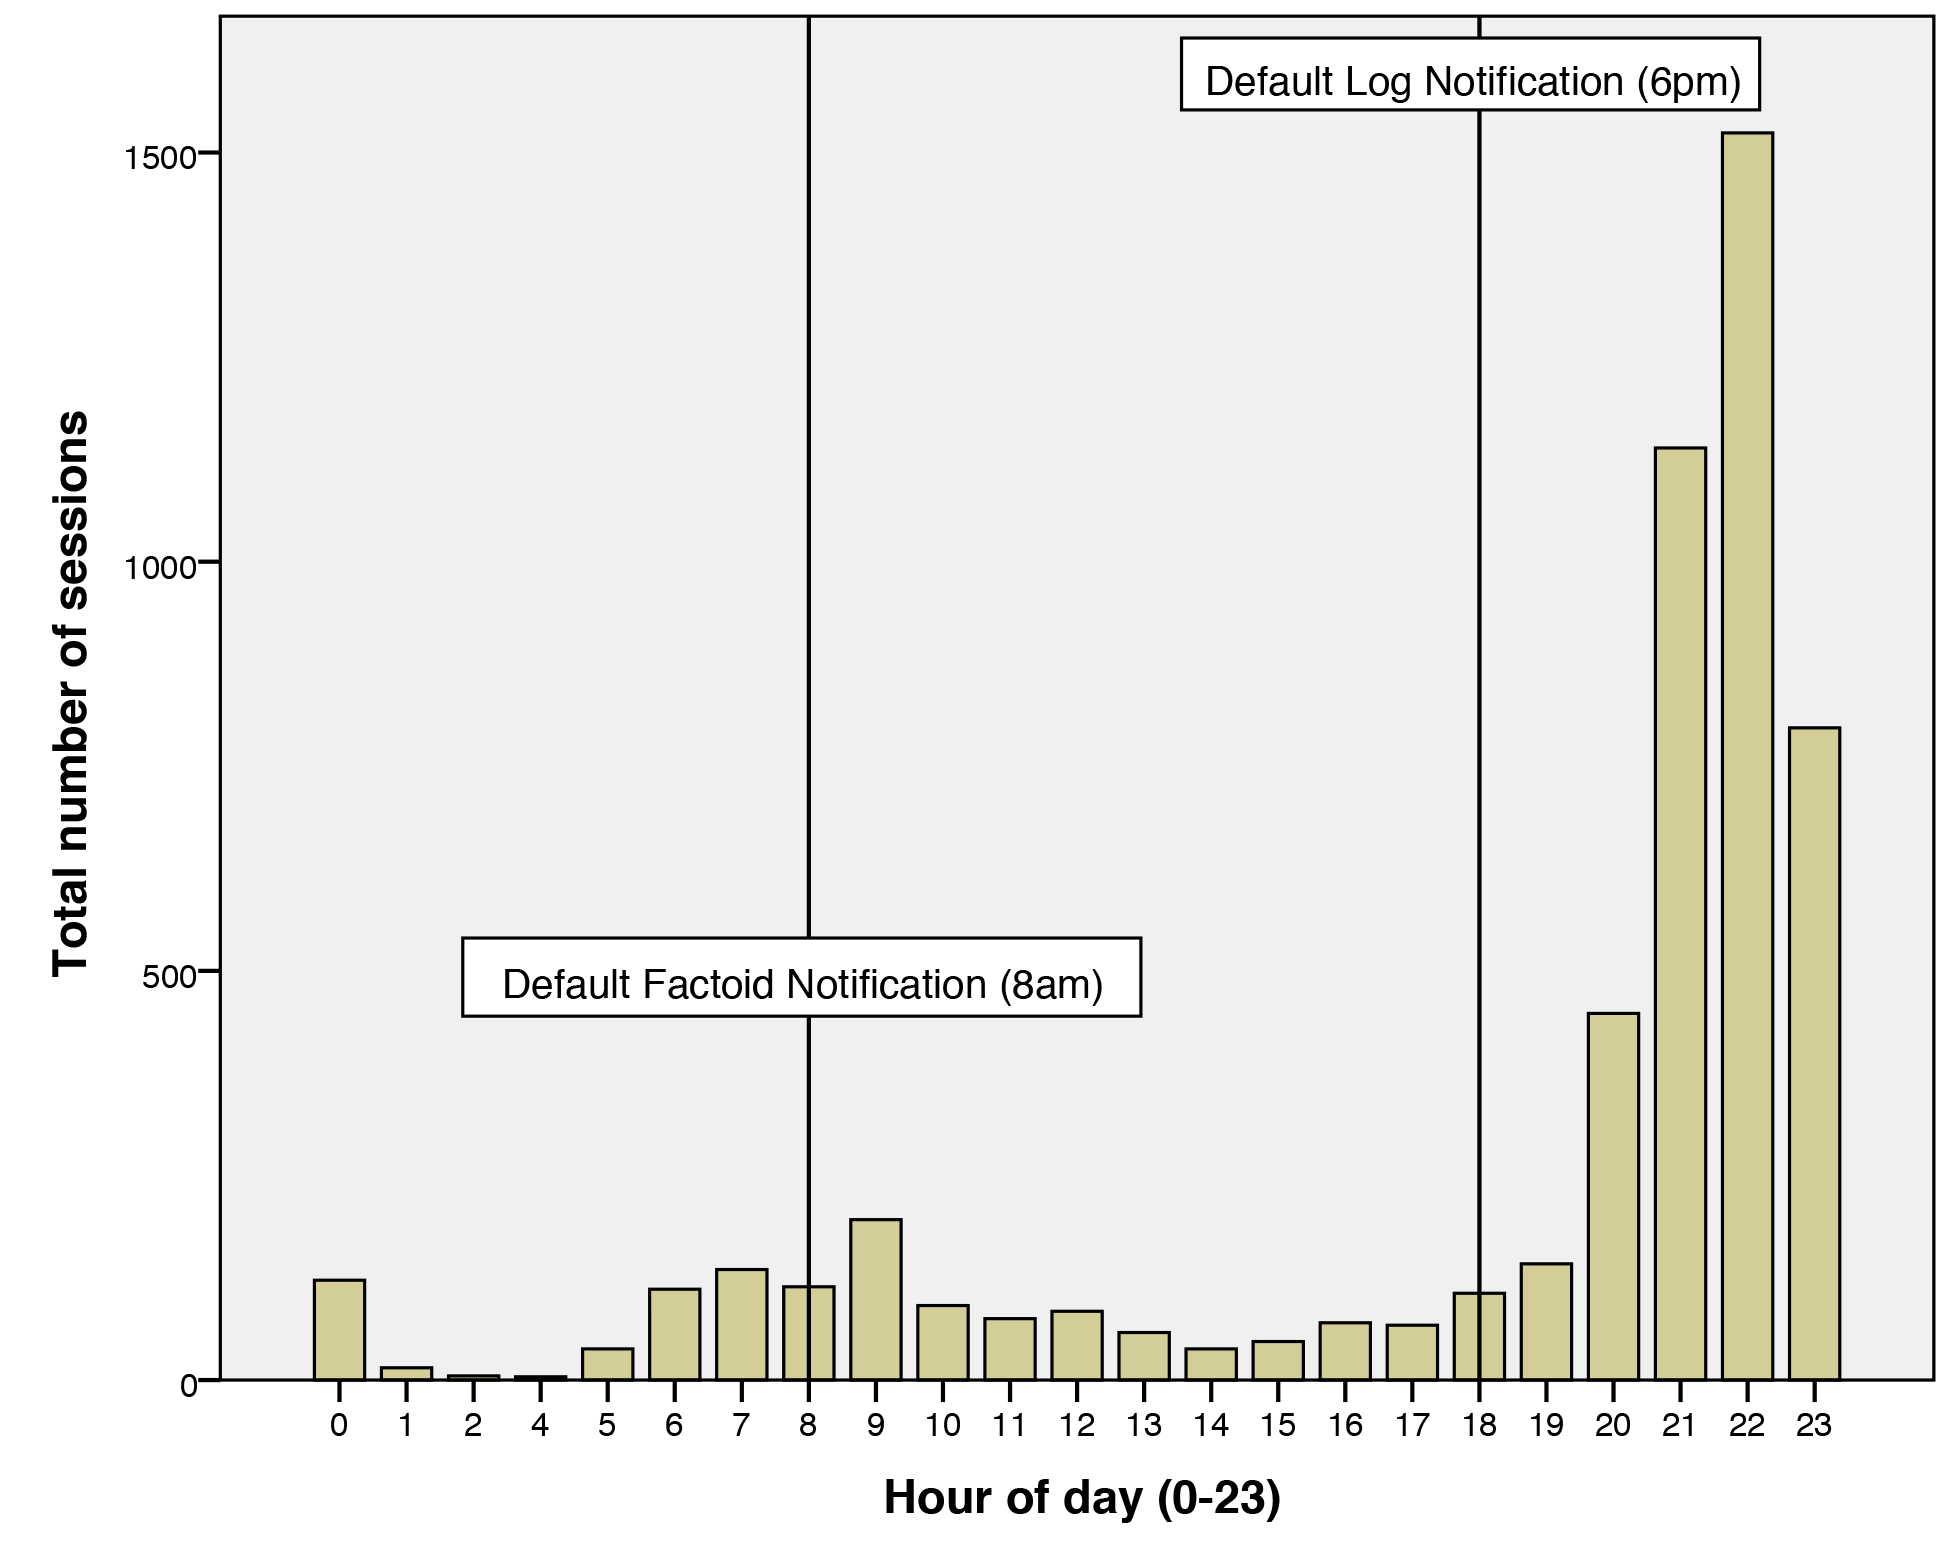
\includegraphics[scale=0.18, angle=0]{Files/prevention-study-3/figures/hour-of-day}
    \caption{Bar graph showing the typical hours of use, with morning activity around the default daily fact notification time at 8am, and activity peaking at 10pm, 4 hours after the default log notification time.}
    \label{fig: time-of-day}
\end{figure}

An additional explanation to these observations may be due to notifications, for which the app was distributed with 2 default times. The first notification was issued in the morning at 8 am, which reminded the user to check their daily fact. The second notification was issued at 6pm, which reminded the user to complete the questions in the app’s log tab. These times have been highlighted in Figure \ref{fig: time-of-day}.

\section{Platform Assessment by Users}
Upon the close of the study, an exit survey was issued to those in the treatment group. 41 participants completed the survey. The survey acted to gather users’ motivations for behaviour change and thoughts on the various components of the study, how they used them, and where they felt improvements could be made.

\subsection{Reported Usage}
Firstly, users were asked how often they used the app on a daily, weekly and monthly basis. Results are presented in Table \ref{tbl: exit-survey-appusage}. Mean usage figures show that the app was used for approximately 5.5 months, almost twice daily. The largest amount of standard deviation was found in the responses for times per day (3.12).

\begin{table}[h]
\centering
\caption{Respondents' answers to survey question: ``Over the six month Gray Matters intervention period (April 2014 – October 2014), how often did you use the App?"}
\label{tbl: exit-survey-appusage}
\begin{tabular}{@{}llll@{}}
\toprule
              & N  & Mean & Std. Dev. \\ \midrule
Months Used   & 39 & 5.54 & 1.315     \\
Days Per Week & 38 & 6.21 & 1.695     \\
Times Per Day & 38 & 1.66 & 3.122     \\ \bottomrule
\end{tabular}
\end{table}

\subsection{Effect on Motivations}
In addition, the survey acted to glean how the app altered motivations towards various parts of the intervention. The survey revealed that the app motivated users to perform physical activity (Never: 14.6\%, Rarely: 12.2\%, Sometimes: 24.4\%, Often: 31.7\%, All of the time: 17.1\%) and make healthier food choices (Never: 12.5\%, Rarely: 2.5\%, Sometimes: 17.1\%, Often 48.8\% and All of the Time: 17.1\%).

\subsection{Maintaining Effort}
When queried upon the app's effect on their past, current and future behaviours, 46.3\% said they definitely will continue with their physical activity changes, and 31.7\% want to continue and increase their activity; 46.3\% wish to continue their improved eating habits, with 29.3\% wanting to continue and improve.

\subsection{Feature Wishlist}
To improve the overall quality and desirability of the app, users were asked about features that they wish were included in future versions.
68.3\% of users wished that guidelines were based on their ‘current’ health status, 34.1\% wished they could set their own target goals, 53.7\% wished they could focus the daily facts on specific behaviour goals of interest and 51.2\% wished to received text feedback if they had made good progress/no progress. 53.7\% wished they could compare their behaviours with others relative to their age, gender and initial fitness status. Regarding the wearable device and app interaction, 70.7\% of post-study survey respondents wished that their wearable automatically synched to the app.
These requested features further emphasise the need for social and wearable integration, and reflect the observations and recommendations made within the app content-analysis performed in Chapter \ref{chapter: prevention-evaluation}, Section \ref{subsection: content-analysis}.

\section{Behavioural Change}
To determine whether behaviour change occurred within the treatment cohort, the self-reported behaviour logs were analysed for trends and correlations over time.

\subsection{Initial Change}
Preliminary analysis performed at week 14 displayed encouraging results, showing that weekly averages across all participants for each behavioural question were increasing, or decreasing, in favourable directions. Of particular interest were the  cognitively stimulating activities ($\beta$ = 0.81, p =.001), social engagement levels ($\beta$ = 0.70, p = .008), perceived stress levels ($\beta$ = 20.81, p = .001), and vigorous physical activity ($\beta$ = 0.88, p = .001) \cite{Norton2015-TRCI}, which have been presented in Figure \ref{fig: preliminary-analysis}. These initial changes were highly encouraging and display that the users were traversing the processes of the action phase in the TTM. Nevertheless, these levels of improvement were expected to slow and eventually plateau given that the room for improvement will continually decrease. Once this occurs, the participants are expected to enter the maintenance phase, ensuring continual practice of their efforts and actively avoiding relapse.

 \begin{figure}[h]
    \centering
    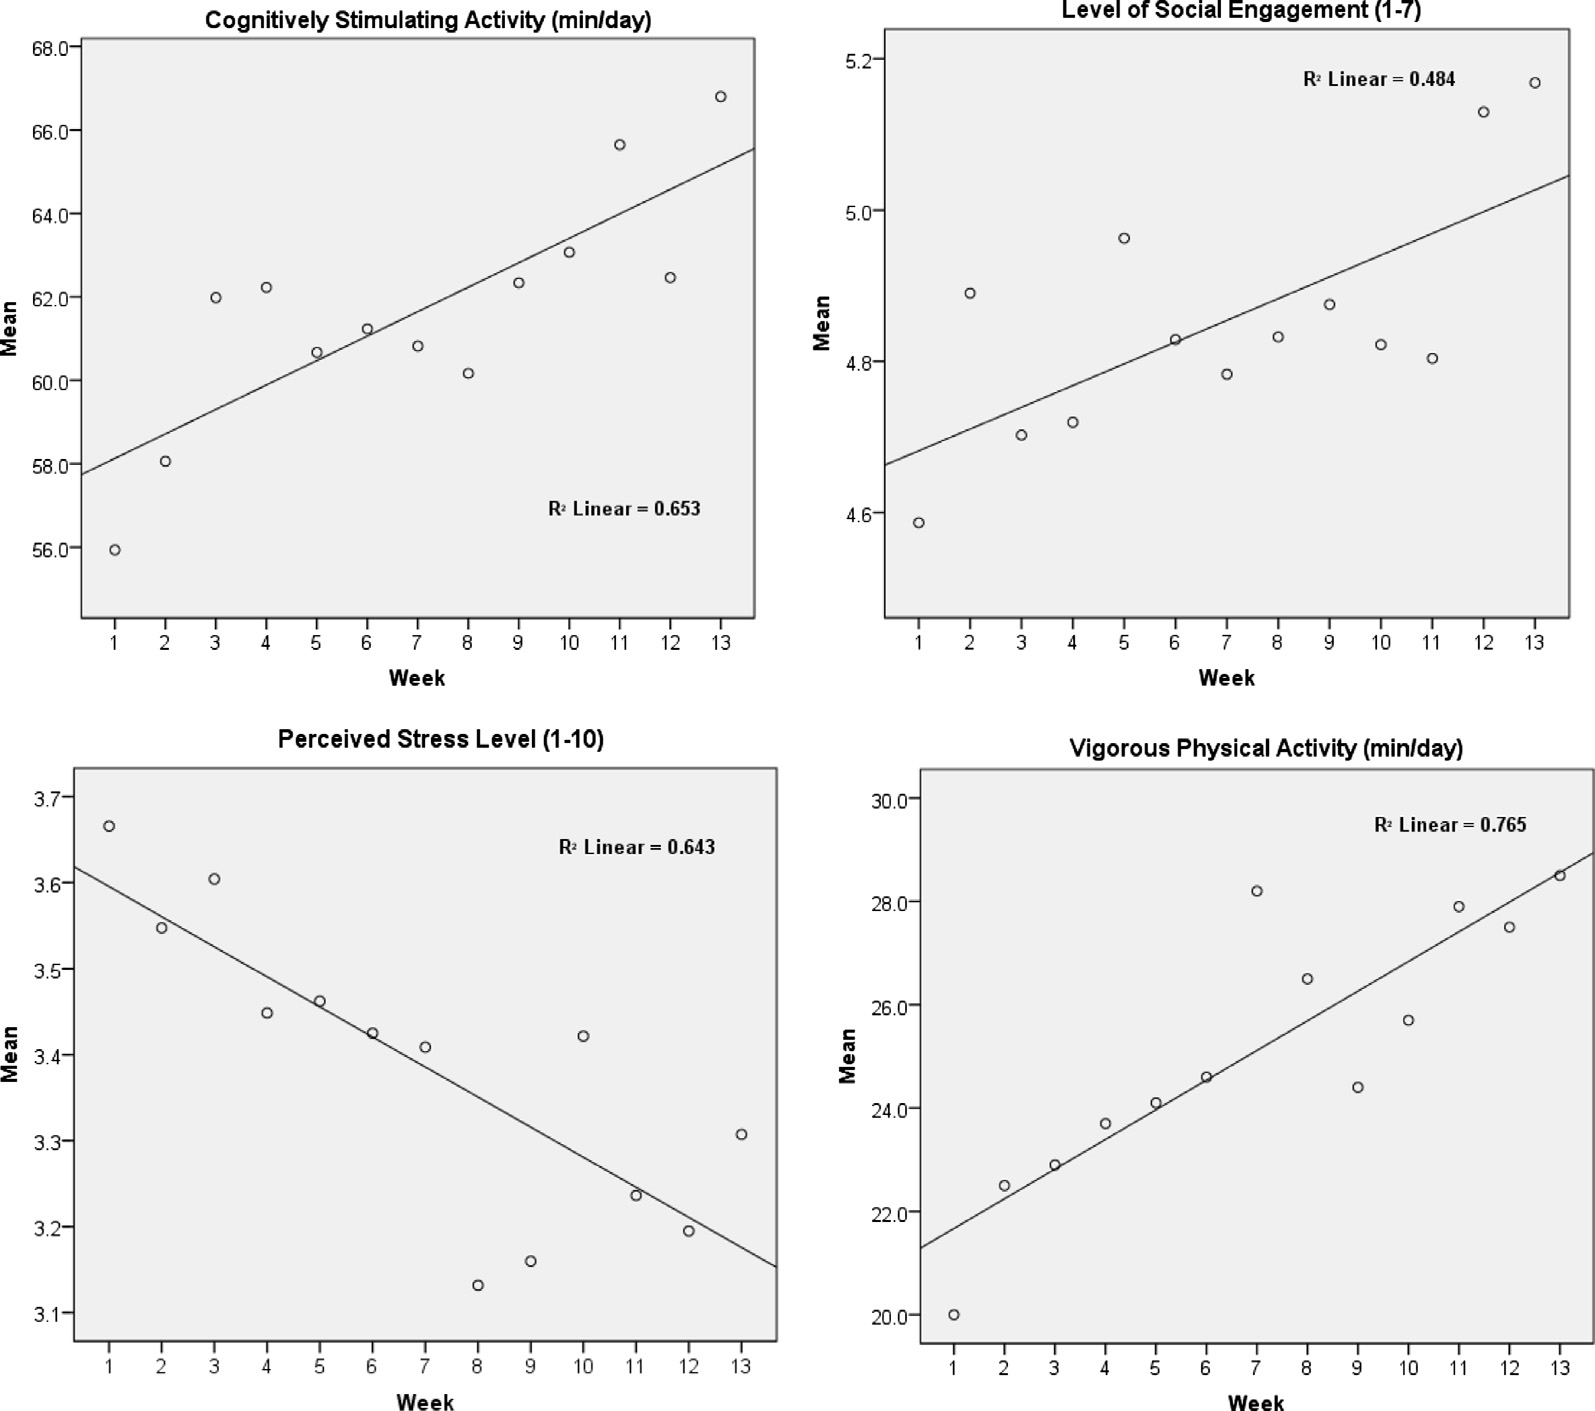
\includegraphics[scale=0.25, angle=0]{Files/prevention-study-3/figures/behaviourchange-week14}
    \caption{Weekly averages of four daily behavioural levels (averaging daily values within each week) for cognitively stimulating activities ($\beta$ = 0.81, p = .001), social engagement levels ($\beta$ = 0.70, p = .008), perceived stress levels ($\beta$ = 20.81, p = .001), and vigorous physical activity ($\beta$ = 0.88, p = .001); all coefficients are standardised.}
    \label{fig: preliminary-analysis}
\end{figure}

\subsection{Progression and Maintenance}
At the close of the study, it was possible to have a full picture of how each participant's behaviour changed over the 26 week period.
To study this change at a high level, the mean performance of achieving the recommended values, across all domains, was calculated on a week-by-week basis for each participant. These individual values were then combined to establish the mean performance of the entire treatment cohort, for each week, across the 26 week period. To account for the varying levels of performance observed in the study, 2 forms of performance value were calculated for each log:

\begin{enumerate}[noitemsep,topsep=0pt]
\item Mean performance not accounting over-achievement; Performance max value fixed to 100\% (Limited).
\item Mean performance allowing for over-achievement; No fixed upper limit. (Not limited).
\end{enumerate}

\subsubsection{Correlation}
Bivariate correlation analysis showed a significant strong positive relationship between the week and mean performance in values which were limited (r = .832, p = \textless .000). There was also a significant strong positive relationship found between the week and mean performance in values which were not limited (r = .776, p = \textless .000).
%VIVA: Chris - There are probably other bi-variate and indeed multivariate analyses you could have pefroemd.  Be prepared to discuss these during your exam and be able to defned why you only considered bivariate analyses

\subsubsection{Linear Regression}
Linear regression analysis shows that the number of weeks using the app explain a significant amount of the variance in the performance scores, limited [F(1, 24) = 54.007, p = \textless.000, R\textsuperscript{2} = .692, R\textsuperscript{2}\textsubscript{Adjusted} = .68], and not limited [F(1, 24) = 36.402, p = \textless.000, R\textsuperscript{2} = .603, R\textsuperscript{2}\textsubscript{Adjusted} = .586], respectively. Visual plots of these regression lines are presented in Figure \ref{fig: performance-linear-limitcomparison}.

\begin{figure}[h]
    \centering
    \begin{subfigure}[t]{0.48\textwidth}
        \centering
        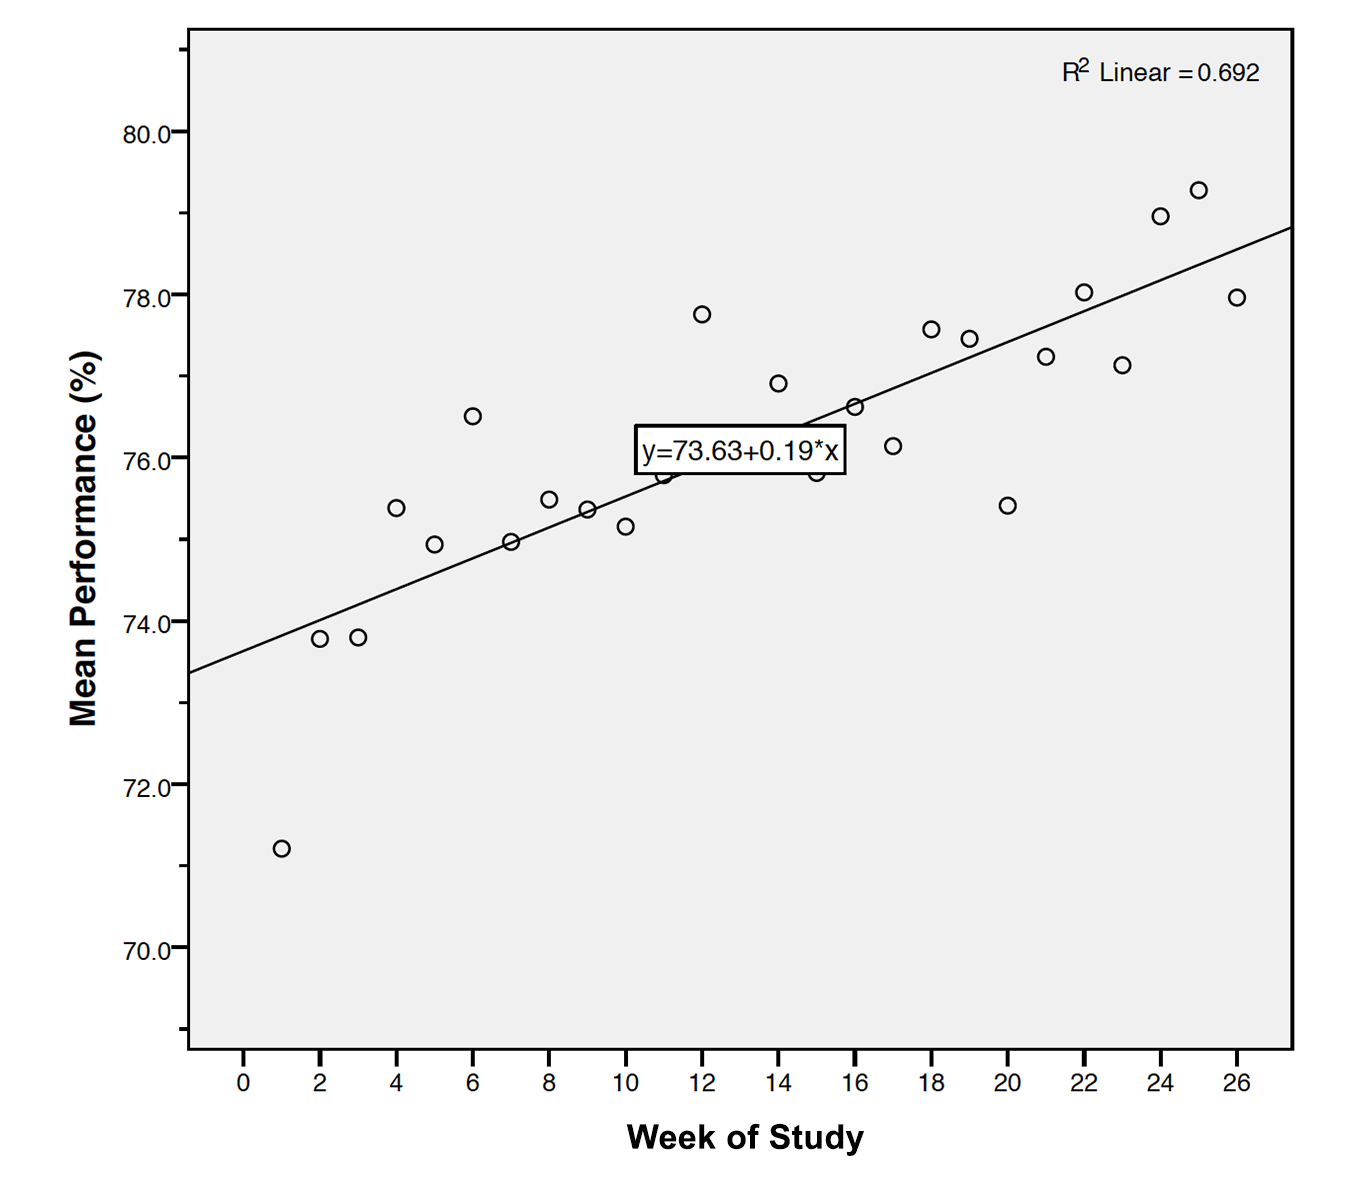
\includegraphics[width=\textwidth]{Files/prevention-study-3/figures/performance-linear-limit}
        \caption{}
        \label{fig: performance-linear-limit}
    \end{subfigure}
    \hfill
    \begin{subfigure}[t]{0.48\textwidth}
        \centering
        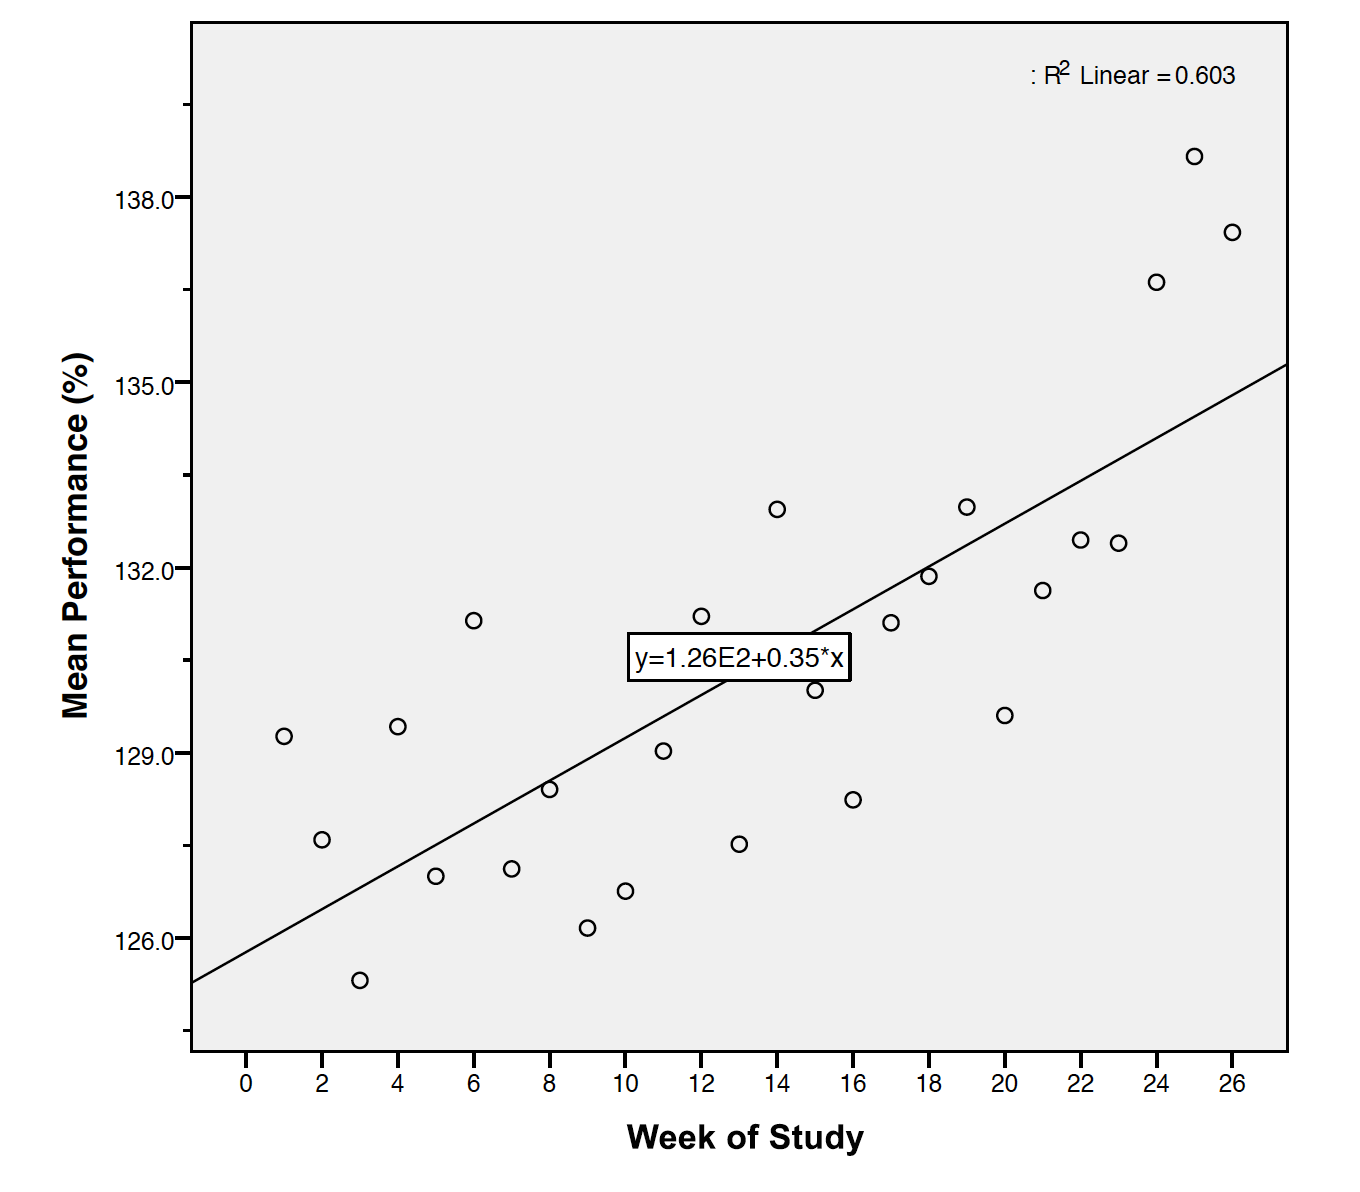
\includegraphics[width=\textwidth]{Files/prevention-study-3/figures/performance-linear-nolimit}
        \caption{}
        \label{fig: performance-linear-nolimit}
    \end{subfigure}
    \caption{Scatter plot showing performance scores (limited (A) and not (B)) against Week number with fitted linear regression lines.}
    \label{fig: performance-linear-limitcomparison}
\end{figure}

\textbf{Limited variables.}
For each additional week, recommended guideline achievement performance increased by 0.189\%. The linear regression equation is as follows:
\begin{equation}
Performance = 73.63 + \left(0.189 \times Week\right)
          \label{eq: calc-performance-limited-behaviour-change}
\end{equation}

Using such a model, to achieve the full 100\% consistently, the participant would need to be actively engaged in the process for \textbf{139.523} weeks. Such an achievement is highly unrealistic, yet this model provides an insight into the time and effort commitment required of persons seeking to positively change their behaviours.

\textbf{Not limited variables.}
For each additional week, recommended guideline achievement performance increased by 0.347\%. The linear regression equation is as follows:
\begin{equation}
Performance = 125.772 + \left(0.347 \times Week\right)
          \label{eq: calc-performance-notlimited-behaviour-change}
\end{equation}

Using such a model, to achieve 100\% consistently, the participant would need to be actively engaged in the process for \textbf{0} weeks. Obviously such a model is unrealistic and skewed, which exposes the issues arising from the use of scores which were not limited to 100\% in the analysis. The root of this issue lies with the variation measurement types used in the behavioural questions. Qualitative questions such as rating stress levels and social engagement, were within a fixed scale (for example, 0-10), and as such it was impossible to `over-achieve' in these measures. Quantitative measures, however, such as physical activity and dietary behaviours, allowed for the entry of values which were above the recommended levels, thus allowing participants to over-achieve. This unbalanced ability to over-achieve in certain domains, and not in others, greatly diminishes the use of any achievement percentages over 100\%. As such, only answers limited to 100\% are considered for further analysis.

\subsubsection{Non-linear regression}
Despite the significance found within correlation analysis (r = .832, p = \textless .000) and a good fit within linear regression (R\textsuperscript{2} = .603, p = \textless.000), behaviour change is a very individual process, during which levels of achievement are expected to peak, plateua, re-adjust, and improve again. Such changes were evident in the observed data shown in Figure \ref{fig: performance-linear-limitcomparison}. As such, the relationship between the week, and level of achievement experienced may be non-linear, and so the linear regression model above may not be the best fit. Due to the changes observed in the data, in particular the observation of plateauing and subsequent improvement, cubic regression was identified as a possible means to model the data. A comparison of the linear and cubic regression lines fitted to the data are presented in Figure \ref{fig: performance-cublic-linear-limited}.
 \begin{figure}[h]
    \centering
    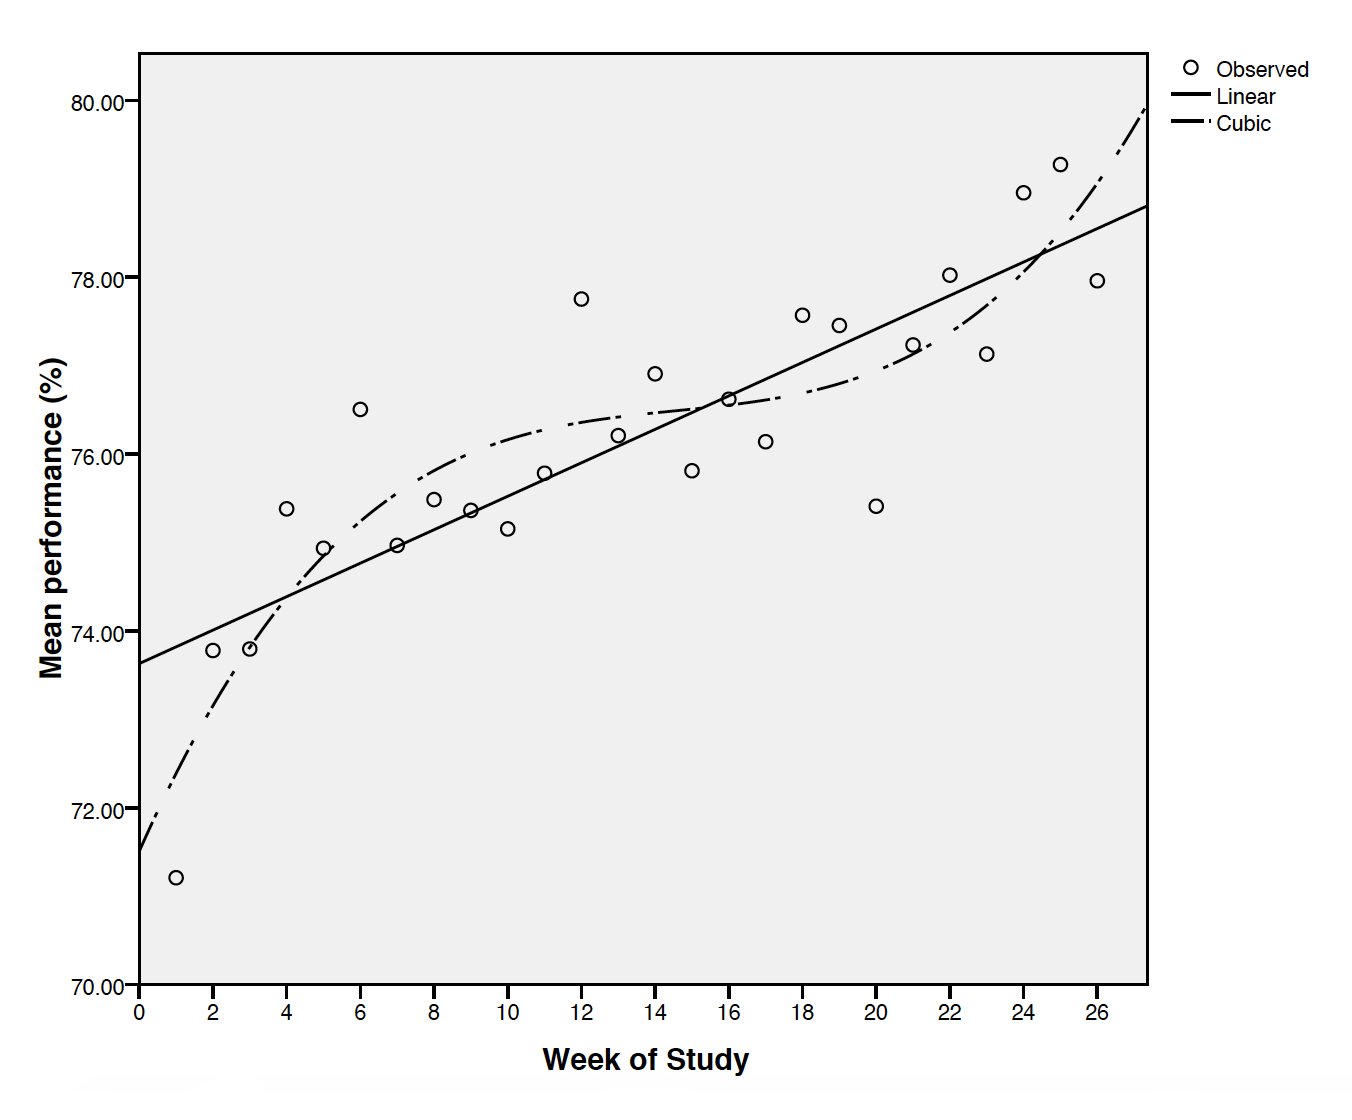
\includegraphics[scale=0.25, angle=0]{Files/prevention-study-3/figures/performance-cublic-linear-limited}
    \caption{Comparison of linear (R\textsuperscript{2} = .603, p = \textless.000) and cubic regression (R\textsuperscript{2} = .784, p = \textless.000) lines fitted to mean behaviour change observed over 26 weeks.}
    \label{fig: performance-cublic-linear-limited}
\end{figure}
The cubic regression model provides a closer fit to the observed data [F(3, 22) = 26.671, p = \textless.000, R\textsuperscript{2} = .784, R\textsuperscript{2}\textsubscript{Adjusted} = .755], than the previous linear model. Within this model, the cubic regression equation is as follows:
\begin{equation}
Performance = \left(0.01 \times Week\right)^{3} +  \left(0.062 \times Week\right)^{2} +  \left(9.41 \times Week \right) +  71.508
          \label{eq: calc-performance-notlimited-behaviour-change}
\end{equation}

Using this equation, a participant is predicted to reach 100\% performance in achieving recommended behaviours related to AD risk for all domains after approximately 40 weeks of effort. To achieve such a goal would be an impressive feat, as adherence to recommended guidelines is typically very low. In the United Kingdom only 35\% of men and 24\% of women achieve the recommended targets for moderate-intensity activity \cite{Miles2007}.

\subsection{Additional analysis}
During the analysis of behavioural data, it became apparent that certain internal components of the study, namely booster events, may of have had an effect on behaviours, as did certain external factors \cite{Hartin2015-ICOST}.

\subsubsection{The effect of booster events}
To analyse the effect that booster events may have on behaviours, a list of events and attendees were analysed. For each attendee at an event, their log responses to the relevant domain questions were compared one week (7 days) prior and post attendance. A Paired-sample t-Test between pre-post attendance highlighted a significant change at the p \textless 0.05 level in domain relevant behaviours for 7 of the 46 events \cite{Hartin2015-ICOST}. Additional detail of these 7 events, including event titles, domains, descriptive statistics of relevant behaviours are presented in Table \ref{tbl: booster-significance}. It must be noted that not all booster events had the desired effect in the observed short term. For example, attendees of events 4 and 15, reported significantly less effort and activity after attending the booster events. For these cases it may be assumed that the attendees felt they overachieved in these areas through attending the event, and reduced their conscious efforts in the following week. Further work is required to test this assumption.

\begin{sidewaystable}
\centering
\caption{List of booster events which resulted in a significant difference in behaviours after attendance.}
\label{tbl: booster-significance}
\resizebox{\textwidth}{!}{%
\begin{tabular}{@{}llllllllll@{}}
\toprule
Event ID \# & Booster Event Activity & Domain & Question & \begin{tabular}[c]{@{}l@{}}Mean \\ (Pre)\end{tabular} & \begin{tabular}[c]{@{}l@{}}Mean \\ (Post)\end{tabular} & \begin{tabular}[c]{@{}l@{}}Std. Dev \\ (Pre)\end{tabular} & \begin{tabular}[c]{@{}l@{}}Std. Dev \\ (Post)\end{tabular} & \begin{tabular}[c]{@{}l@{}}Sig.\\ (2-Tailed)\end{tabular} & \begin{tabular}[c]{@{}l@{}}Num.\\ Attendees\end{tabular} \\ \midrule
4 & Mindfulness & Stress & Self effort to decrease stress & 4.43 & 5.73 & 2.10 & 1.63 & 0.03 & 5 \\
15 & Learning to paint & Mental & Cognitively stimulating activity (mins) & 73.67 & 64.52 & 28.83 & 24.06 & 0.03 & 11 \\
24 & Intro to  Pilates & Physical & Vigorous physical activity (mins) & 24.69 & 25.88 & 16.81 & 13.39 & 0.046 & 9 \\
25 & Pilates Reformer & Physical & Moderate physical activity (mins) & 41.25 & 43.11 & 2.84 & 19.11 & 0.021 & 3 \\
29 & Yummy dips for fresh veggies & Food & Fruits and veg consumption (cups) & 3.63 & 4.49 & 1.24 & 1.39 & 0.038 & 6 \\
33 & Relationship Enrichment & Social & Self-rate stress level & 3.03 & 2.38 & 1.91 & 1.28 & 0.03 & 10 \\
36 & Salads and Stir-fry & Food & Nuts, seeds, or legumes consumption (cups) & 1.32 & 1.68 & 0.68 & 0.87 & 0.029 & 7 \\ \bottomrule
\end{tabular}}
\end{sidewaystable}

\subsubsection{The effect of weather conditions}
In addition to internal study components, a number of external factors were also analysed for effect, such as public holidays and local weather conditions.
Analysis of local weather conditions resulted in a finding of positive correlation between local temperature in the Cache County area with physical activity, both moderate and vigorous, R = 0.585, R = 0.725, respectively \cite{Hartin2015-ICOST}. Figure \ref{fig: scatter-regression-temp-activity} shows that as local temperature increases, vigorous physical activity also increases.
%VIVA: Chris - Did you consider any multi-variate analyses at all?  If not can you justify this?  Perhaps you could run a very quick multi-variate analysis after you submit and you could bring the results with you to the oral exam?

\begin{figure}[h]
    \centering
    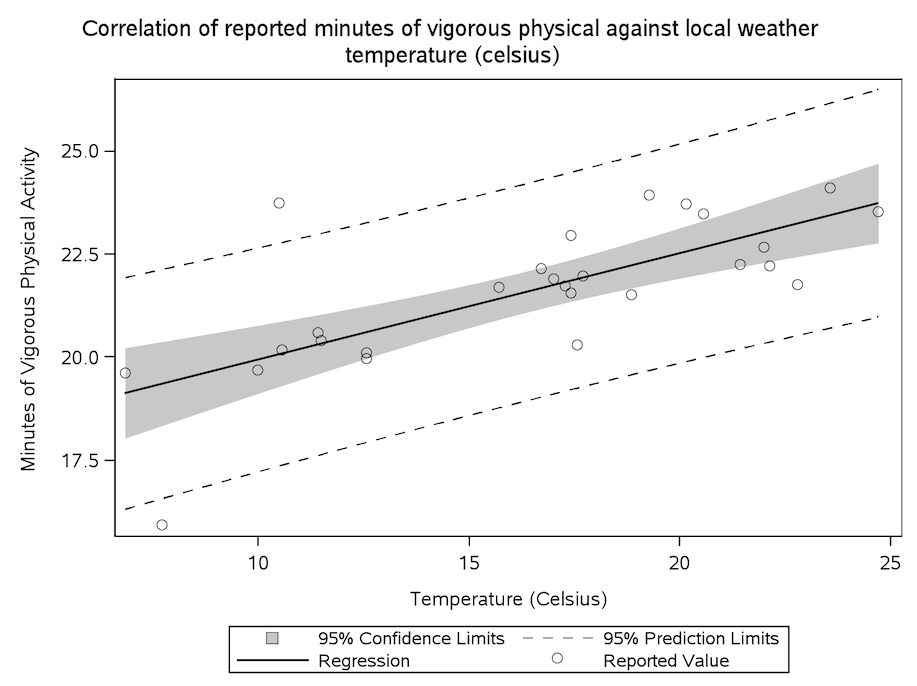
\includegraphics[scale=0.4, angle=0]{Files/prevention-study-3/figures/correlation-temp-activity}
    \caption{Scatter plot showing correlation analysis of participant’s self-reported vigorous exercise against the external factor local average temperature in degrees Celsius (R = 0.725, p = \textless.0001).}
    \label{fig: scatter-regression-temp-activity}
\end{figure}
%VIVA: Chris - What are you using as the threshold for R in regression to indicate a good fit?

\section{Clinical Outcomes}
Whilst behaviour change was shown to occur within individuals in the study, the effect on their health outcomes must still be determined. As shown in Table \ref{tbl: clinical-variables}, a number of biological and clinical markers were taken from each participant at the beginning and at the end of the study. This data has been processed and analysed for trends and correlations. In addition, this clinical data has also been paired with the previously discussed app usage and behavioural datasets, from which a number of hypothesises are developed and tested.

\subsection{Number of times app used per week}
Logically, it is hypothesised that increased exposure to the app and its material would result in favourable outcomes, both in behaviour change and in clinical markers.
\subsubsection{Method}
Firstly, the number of times that the app was launched per week was established and categorised into groups (\textless1, 1-3, 3-5, 5-7, 7+ per week). These groups were then evaluated with various clinical and biometric measurements taken from the participants at the start and end of the study, along with the control group.
\subsubsection{Results}
From a high-level, it is evident that increased app exposure has an observable effect in various clinical measurements, with particularly observable effects within BMI and systolic blood pressure (SBP) measurements, shown in Figure \ref{fig: applaunch-bmi} and Figure \ref{fig: applaunch-bp}, respectively.

\begin{figure}[h]
	\centering
    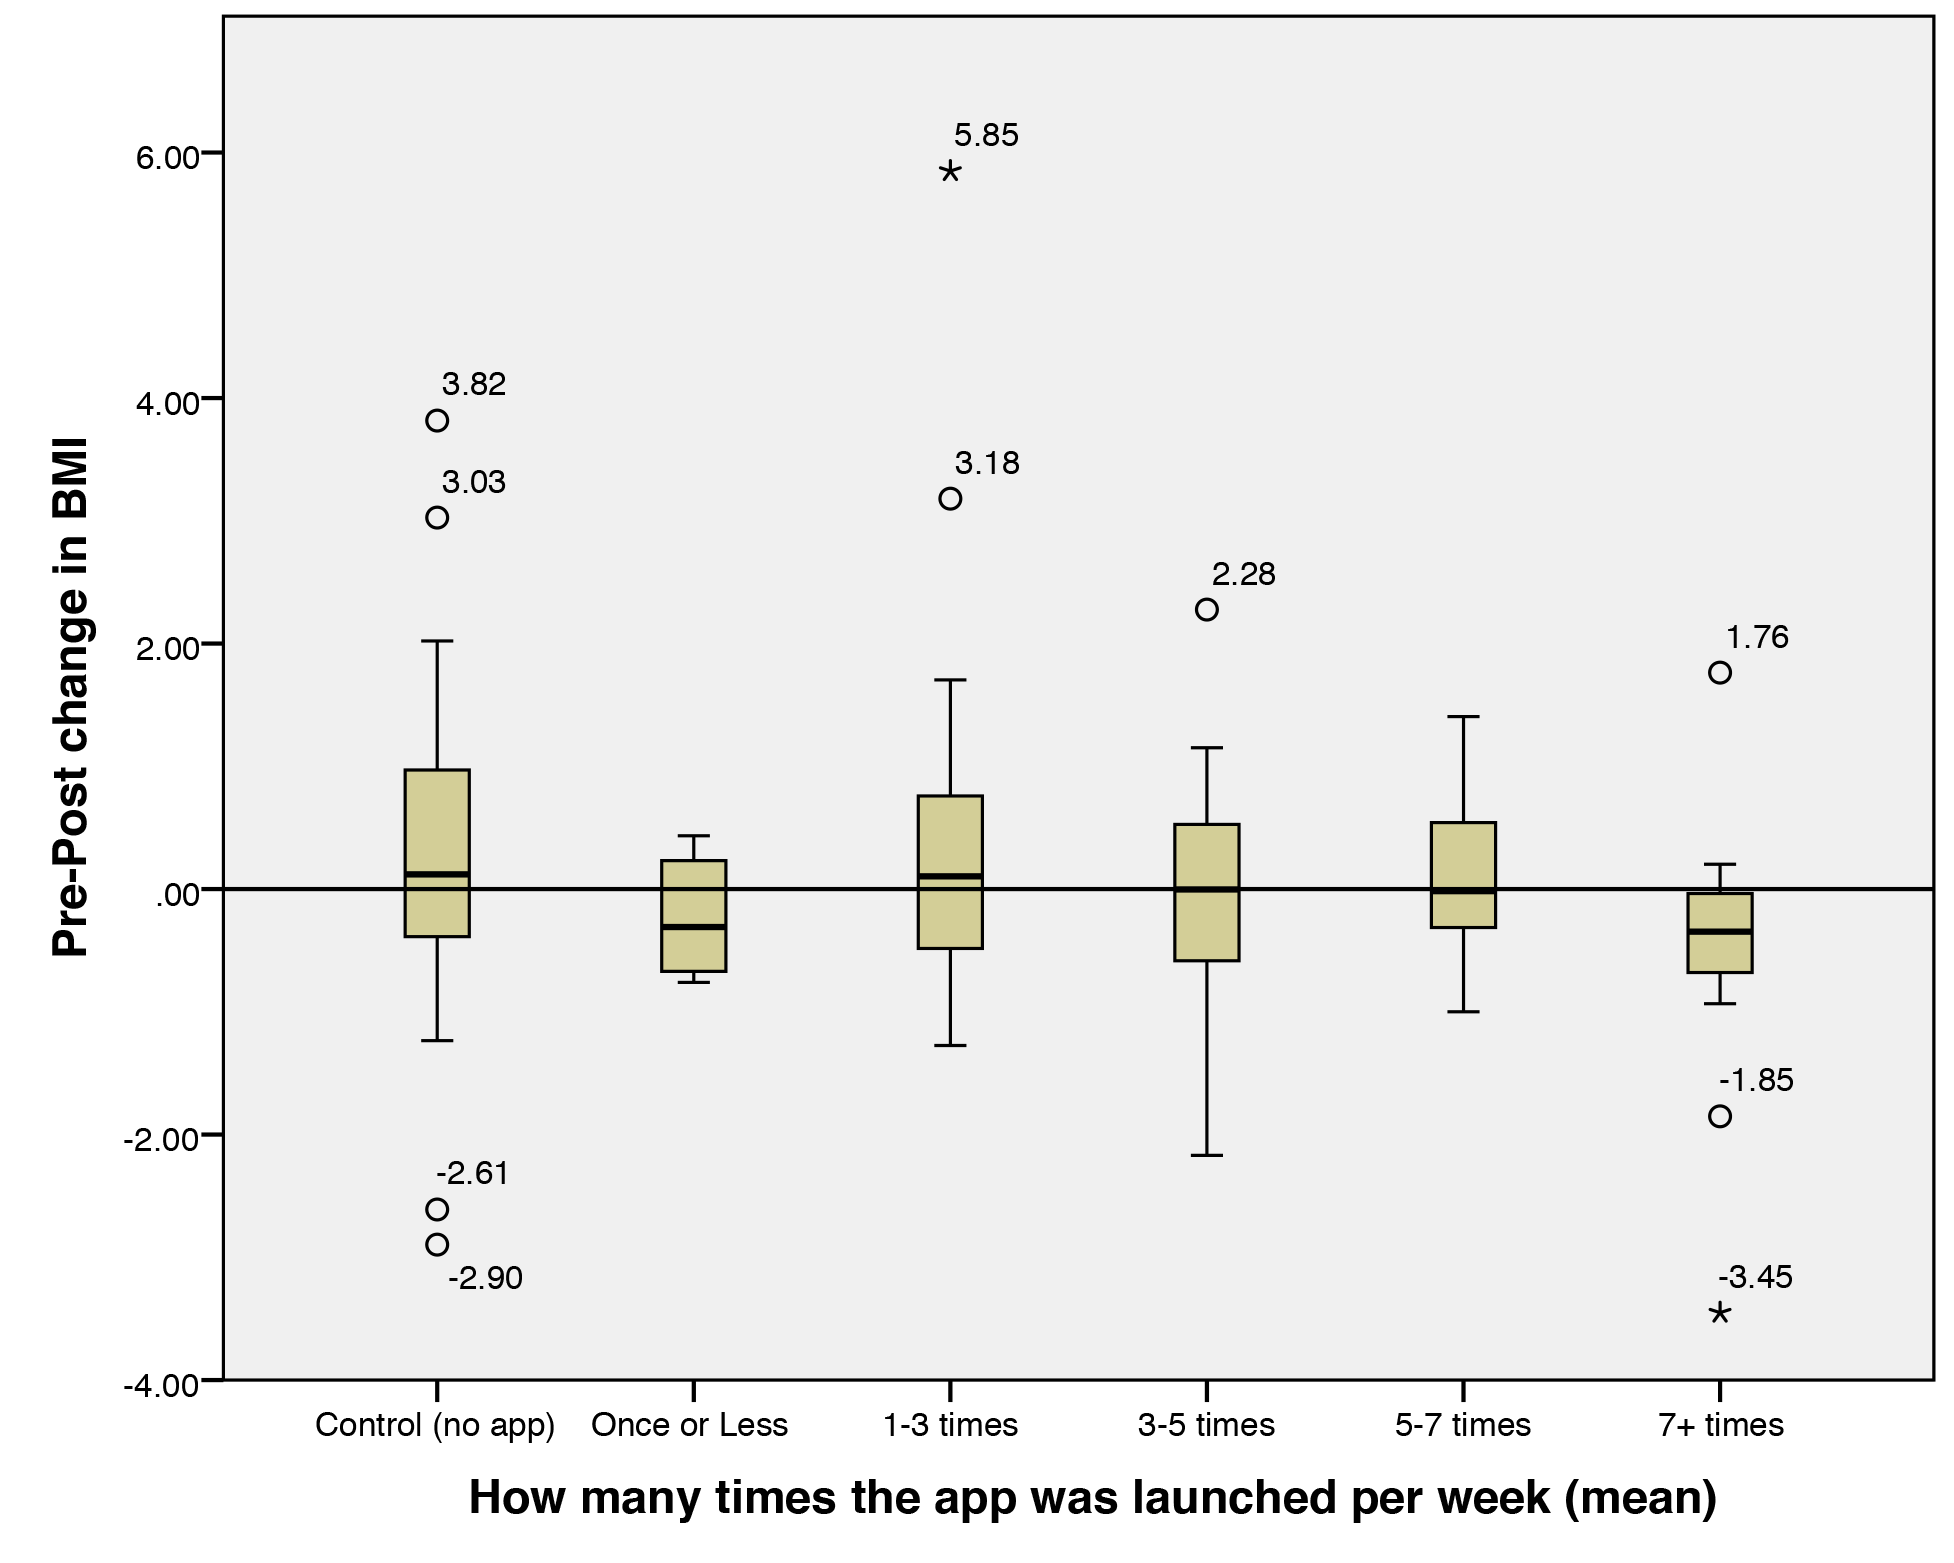
\includegraphics[scale=0.18, angle=0]{Files/prevention-study-3/figures/applaunch-bmi}
  	\caption{Boxplot showing no app (control) and grouped app launches per week (treatment) against observed changes in BMI. Outliers are plotted as individual points.}
    \label{fig: applaunch-bmi}
\end{figure}

\begin{figure}[h]
	\centering
    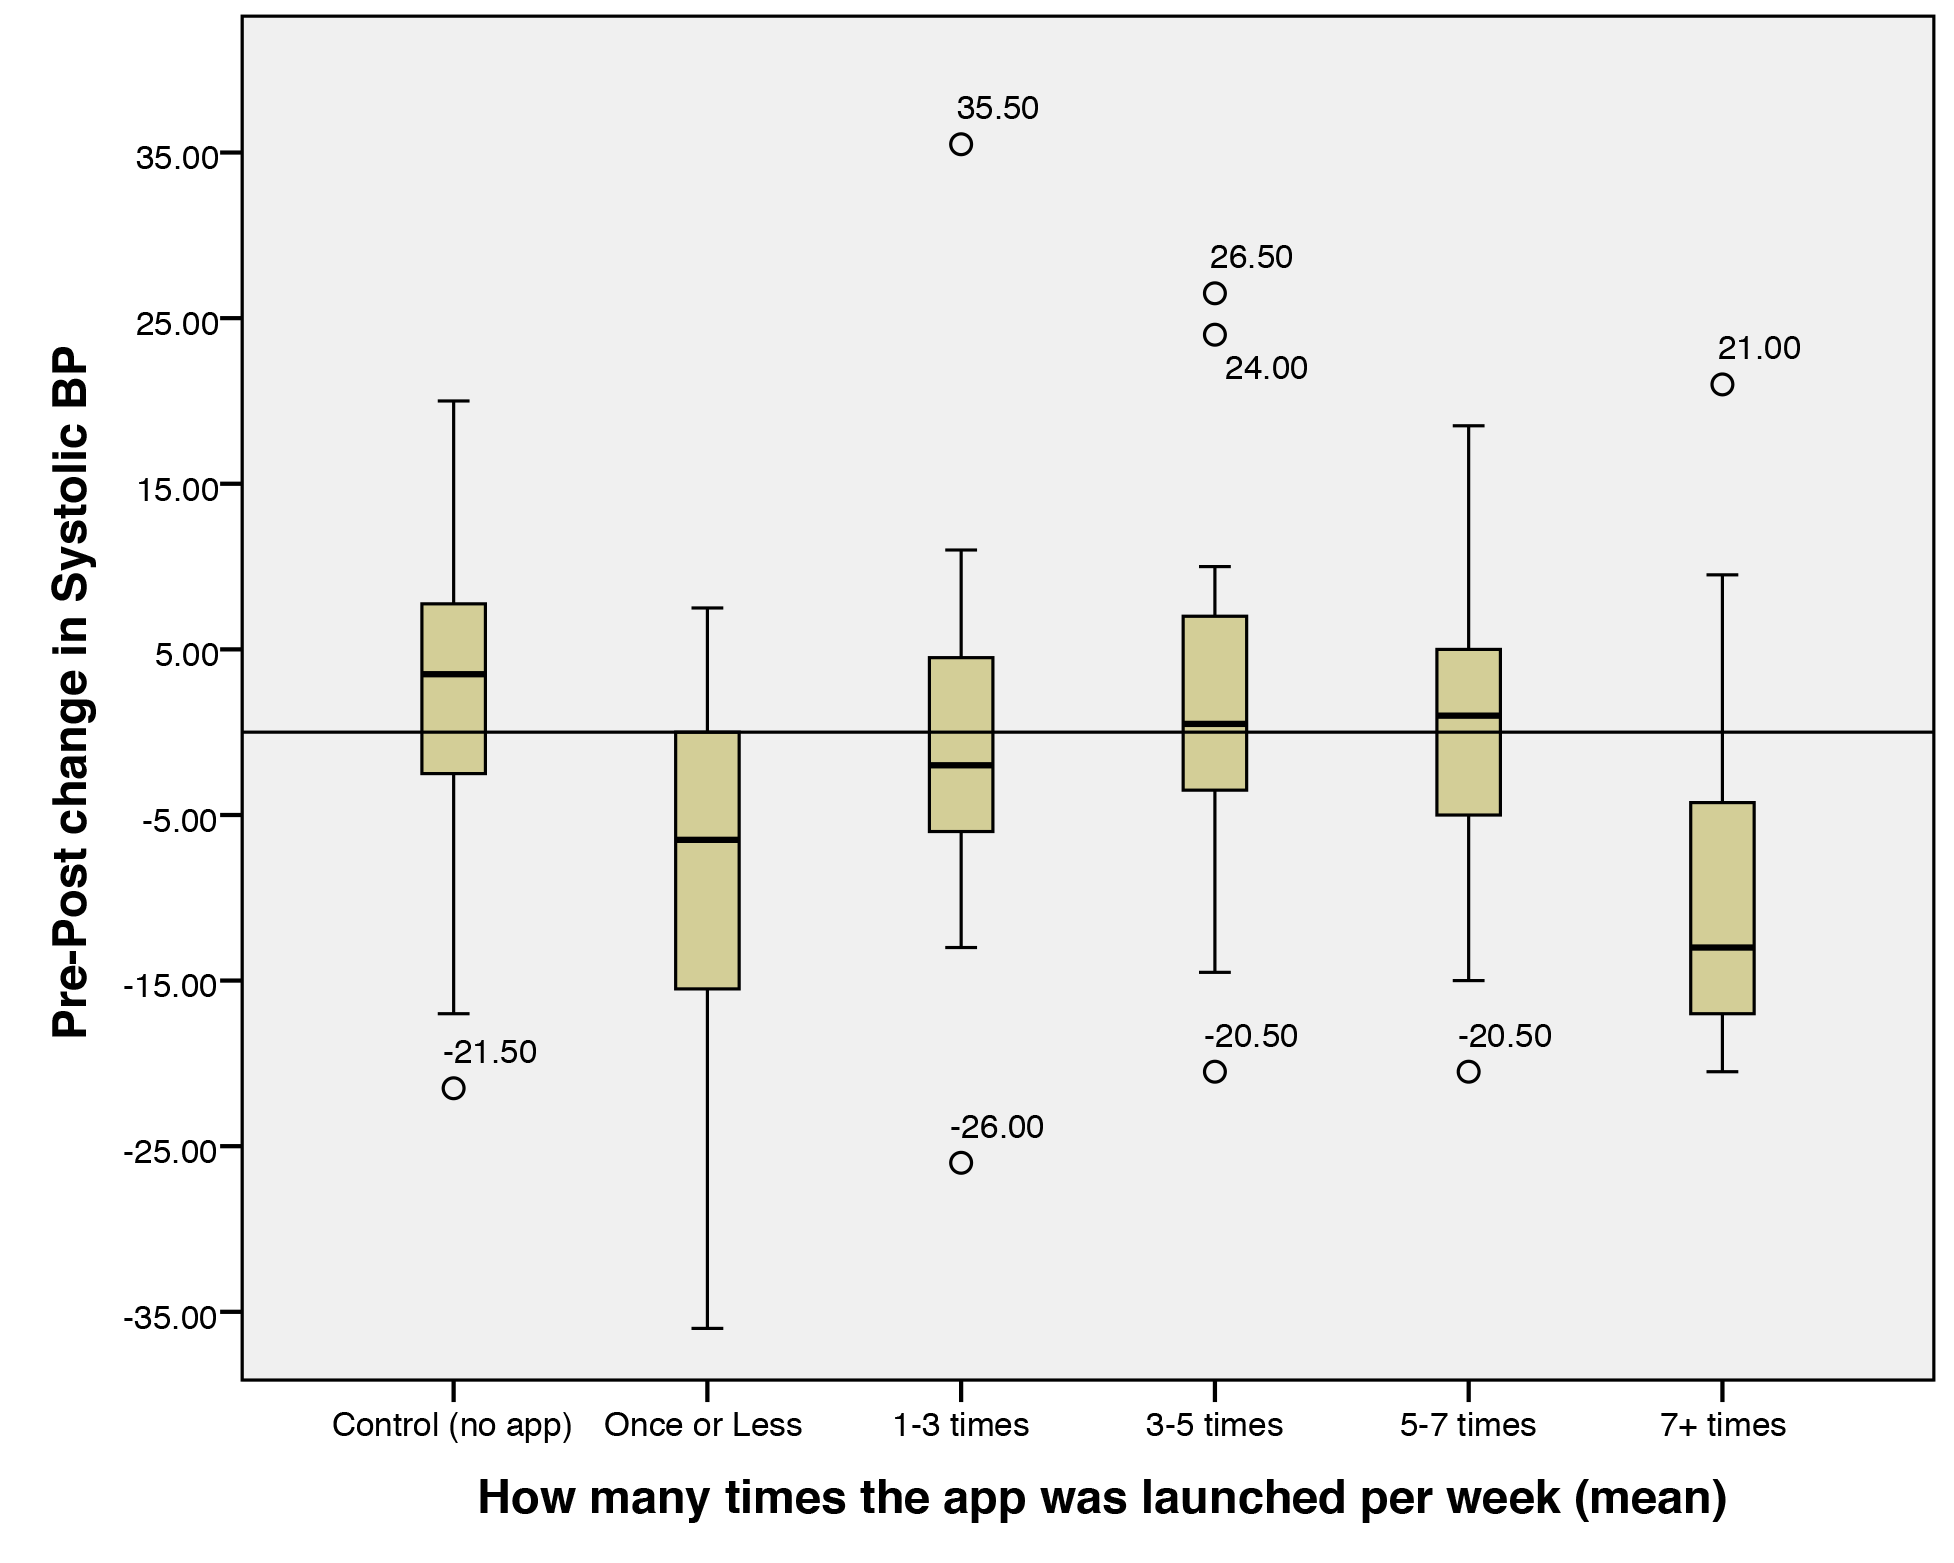
\includegraphics[scale=0.18, angle=0]{Files/prevention-study-3/figures/applaunch-bp}
  	\caption{Boxplot showing no app (control) and grouped app launches per week (treatment) against observed changes in systolic blood pressure (mm/Hg). Outliers are plotted as individual points.}
    \label{fig: applaunch-bp}
\end{figure}

It is evident that the control group have undesirable increases over the intervention period, whilst the treatment group have sustained or reduced their measurements. Notably, those who looked at the app \textit{greater than 7 times per week} appear to have the largest reduction in BMI and blood pressure, whilst those less than 7 times and greater than 1 vary in their results \cite{Hartin2015-JMIR}. It is also interesting to note that those who looked at the app once or less per week also maintained favourable rates of decline. It is proposed that these users are self-sufficient in their efforts to enact behaviour change and do not require the app to aid them.
%VIVA: Chris - is is an interesting point that I would agre with.  One size does not fit all

\subsection{Compliance to log-entry}
The average number of logs completed per day were analysed for correlations to the clinical changes observed in the study, suggesting the following hypothesis:
\begin{description}
  \item[H1] The number of logs completed each day will correspond to greater change in clinical and biological markers.
  \item[H0] There is no supported relationship between daily log and clinical or biological markers.
\end{description}

\subsubsection{Method}
The clinical measurements were analysed as both their raw values, as continuous variables, and also as dichotomous groups. Using domain knowledge, these groups were classed as showing Improvement or No Improvement post intervention.
\subsubsection{Results}

\textbf{Continuous Variables.}
Analysis shows that daily log completion rates show no relationship between pre-post BMI scores (r = .016, p = .872) and diastolic blood pressure (r = .064, p = .523). There was weak positive correlation found in systolic blood pressure (r = .28, p = .784), and weak negative relationships in resting heart-rate (r = -.121, p = .23) and blood carotenoids (r = -.105, p = .294). Further correlation analysis was completed on the biological markers, which also showed positive, however, weak, correlation between the number of logs completed and pre-post total cholesterol (r = .145, p = .91) and triglycerides (r = .145, p = .15), and negative, weak, correlation in serum glucose (r = -.88, p = .382) and blood insulin levels (r = -.105, p = .296).
Nevertheless, calculating partial correlation, controlling for the number of days the participant had the app installed, highlighted toward a significant correlation between total cholesterol and average questions per day (r = .193, p = .055). Adding an extra control for the participant’s initial recorded total cholesterol levels resulted in a significant correlation (r = .228, p = .024). We therefore reject the null hypothesis for this particular case.

\textbf{Dichotomous Groups.}
After categorising pre-post results as showing improvement, or not improvement, independent samples t-Tests showed that participants who improved their HDL cholesterol levels during the study duration answered a statistically significant higher number of questions per day (8.30 $\pm$ 2.29) than those with no improvement (6.52 $\pm$ 3.612), t(97.74) = -3.051, p = .003.
%VIVA: Chris - .003 This is a good result! 

\subsection{Achieving recommended daily targets}
As one of the primary methods by which participants were educated about favourable lifestyle behaviours, the recommended daily targets served an important function. In addition, these targets were established using the latest scientific literature. To evaluate the effect of achieving these targets the following hypothesis is tested:
\begin{description}
  \item[H1] The greater number of recommended goals achieved, the larger the degree of change in clinical and biological markers.
  \item[H0] There is no supported relationship between achieving recommended values and clinical or biological markers.
\end{description}

\subsubsection{Method}
Participants’ self-reported behaviours were analysed to find the frequency and percentage of times that they achieved the recommended daily goal value for each question. Once again, in addition to these continuous measures, each pre-post clinical and biological reading was categorised into groups, showing Improvement or No-Improvement.

\subsubsection{Results}
\textbf{Continuous Variables.}
Correlation analysis between a participant’s mean percentage of recommended goals achieved, across the study duration and observed clinical measurement changes showed the following: No relationship for systolic (r = -.013, p = .896) and diastolic (r = -.35, p = .732) blood pressures, and no relationship in carotenoids (r = -.013, p = .895). Positive weak, correlation was found in resting heart rate (r = -.107, p = .285) and also BMI change (r = .157, p = .116). Biomarker changes were also correlated against percentage of recommended values achieved showing: No correlation in serum glucose (r = -.075, p = .455) and blood insulin levels (r = -.049, p = .624). Positive, however, weak correlation was found for pre-post triglyceride values (r = .155, p = .124). Significant correlation, at the 95\% confidence interval, was found in pre-post total cholesterol (r = .217, p = .03). The null hypothesis is accepted for all but this case.

\textbf{Dichotomous Groups.}
For each individual, a base-line performance level was calculated from their self-reported behaviours in their first week of enrolment. Since there were a number of highly active and healthy living individuals within the treatment group, to reduce the ceiling effect on the data, the first quintile (n=20) of participants were removed from the analysis. The ceiling effect can lead to a situation where the averages of comparison groups are skewed by the top or bottom performing participants, which leads the to misattribution of zero effect for the entire groups, despite noticeable differences in the remaining participants\cite{cramer2004sage}.

Using the dichotomous groupings of Improvement and No-Improvement, significant correlations were found between daily goal percentage achieved and BMI reduction (r = .264, p = .017). An independent samples t-Test showed participants who decreased their BMI achieved a significantly higher percentage of attaining their recommended daily goals (56.21 $\pm$ 30.4\%) than those who increased their BMI (40.12 $\pm$ 29.1\%), t(80) = -2.449, p = .017. Further analysis showed that 69.2\% (n=18) of those who achieved a mean performance percentage of 60\% or greater, across all domains, reduced their BMI during the study, whereas 60.7\% (n=34) of those who did not, increased their BMI.

\begin{table}[h]
\centering
\caption{Odds ratio and relative risk analysis for participants who achieved over 60\% of their recommended daily targets (mean) and BMI change outcome.}
\label{tbl: oddsratio-recommendedtargets-bmi}
\begin{tabular}{@{}llll@{}}
\toprule
\multirow{2}{*}{} & \multirow{2}{*}{Value} & \multicolumn{2}{l}{95\% CI for Mean} \\ \cmidrule(l){3-4}
 &  & Lower & Upper \\ \midrule
\begin{tabular}[c]{@{}l@{}}Odds Ratio for Recommended Achieved \textgreater60\% \\ (Achieved / Did Not Achieve)\end{tabular} & .288 & .107 & .774 \\
For cohort BMI change = Increased & .507 & .274 & .936 \\
For cohort BMI change = Decreased & 1.762 & 1.164 & 2.667 \\
N of Valid Cases & 82 &  &  \\ \bottomrule
\end{tabular}
\end{table}

Analysis of cross tabulation, as presented in Table \ref{tbl: oddsratio-recommendedtargets-bmi}, shows that those who achieved over 60\% of their recommended daily goals were 1.762 times more likely to decrease their BMI during the study, or 0.507 times less likely to increase their BMI, than those who did not achieve 60\%.

\subsection{Physical activity levels}
Physical activity levels were assessed in the study through the participants' self-reported behaviours via the following 3 questions:
\begin{enumerate}[noitemsep,topsep=0pt]
	\item Number of minutes performing moderate physical activity
	\item Number of minutes performing vigorous physical activity
	\item Nike fuel points earned via wearable device
\end{enumerate}

Each participant’s results were analysed for correlations between these values and clinical observations. The following hypothesis is tested:
\begin{description}
  \item[H1] The greater number of minutes performing physical activity or greater number of fuel points achieved, the larger the degree of change in clinical and biological markers.
  \item[H0] There is no supported relationship between physical activity levels and/or fuel points with clinical or biological markers.
  \end{description}
%VIVA: Chris - Are these somehow not implicity linked? RE: Fuel points and minutes of activity.

\subsubsection{Method}
Participant's self-reported behaviours in the questions relating to physical activity were analysed. Changes in clinical and biological markers between pre and post intervention, were once again categorised as either showing improvement or no-improvement.
Again, using the base-line performance metric calculated on the first week of observation, participants in the last decile (bottom 10\%) were excluded from the analysis to reduce ceiling effects. 

\subsubsection{Results}
\textbf{Vigorous activity.}
After removal of the last decile, an independent samples t-Test found that the remaining participants (n=92) who decreased their BMI (n=45) reported statistically significantly more vigorous physical activity (23.94 $\pm$ 10.76 minutes) than those who increased their BMI (19.09 $\pm$ 12.36 minutes), t(90) = 2.002, p = .048.
\newline \textbf{Moderate activity.}
Interestingly no correlation was found with moderate physical activity levels and BMI reduction status.
\newline \textbf{Wrist-worn Wearable.}
Again no correlation was found with the number of fuelpoints achieved from the wrist-worn wearable device and BMI reduction status.
%Viva: Chris - This is perhaps due to the measruements only recording general movements throughout the day.  If you were to consider the top grouping of fuelpoints this may have shown a different result.
Nevertheless, upon removing the first quintile, it was uncovered that those who improved their levels of HDL cholesterol during the intervention achieved significantly higher fuelpoints on a daily basis (2569.39 $\pm$ 641.17), than those who observed no improvement (2233.9 $\pm$ 800.34), f(82) = -2.052, p = .043. Literature in the area of endocrinology and metabolism supports this observation as physical exercise is associated with increases in HDL \cite{Franklin2014}.

\subsection{Stress reduction}
Within the literature, stress and its associated physiological resultants are considered valid components of AD risk \cite{Dotson2010,Royall2012,Boyle2010}. As hypertension is present in all major causes of cognitive impairment \cite{Iadecola2014}, it is of particular interest as a measurement when associated with stress and AD risk. As such participant's self-reported stress reduction efforts were analysed for their effect on clinical measures, with specific emphasis on SBP.

\subsubsection{Methods}
Each participant’s SBP were recorded pre and post intervention and categorised into: Low (\textless90), Ideal (90-120), Pre-Hypertension (120-140) and Hypertension (\textgreater140). Those with non-ideal SBP at their pre-intervention recording (n=50) were analysed to observe if a change of category occurred during the intervention. Changes observed in these participants were categorised into 3 groups: Improvement (n=13), No-Improvement (n=14) or Deterioration (n=23).
%VIVA: Are these general categories or are these specific to age ranges?

\subsubsection{Results}
One-Way ANOVA analysis of their category changes showed a significant correlation between efforts to reduce stress (effort rated 1-10: 10 is high effort) and SBP category change as a whole, p = .035 (excluding first quintile of baseline performers). Multiple comparisons of the three groups showed significance between those who had no improvement (3.11 $\pm$ 2.32 effort rating) and those who had deteriorated (5.28 $\pm$ 2.105 effort rating), p = .028. No significant difference was found between improvement (4.18 $\pm$ 1.89 effort rating) and the remaining groups.

\subsection{Demographic Comparisons}
To fully utilise all available data, demographic information was also considered for analysis. To compare overall performance for participants during the study, the \textit{percentage of recommended values achieved} was used as the base metric. In addition, for the entire treatment cohort, each participant was categorised into quintiles based on their percentage of recommended values achieved (1=Highest, 5=Lowest). These performance quintiles were also then compared to a number of demographic variables collected at the start of the study.

\subsubsection{Family History of Alzheimer's Disease}
Analysis of this data showed relationships between a participant’s achieved percentages and if that participant knew of a member of their family having dementia. This relationship is especially true when excluding the 1st quintile, and can be observed visually between the 2nd and 5th quintiles in Figure \ref{fig: family-quintile}. The pattern observed shows that more participants who know of a family member with dementia achieve higher percentages of their recommended values than those who do not. Partial correlation within these quintiles, controlling for number of days enrolled in the study shows significant correlation (r = .232, p = .036).

\begin{figure}[h]
	\centering
    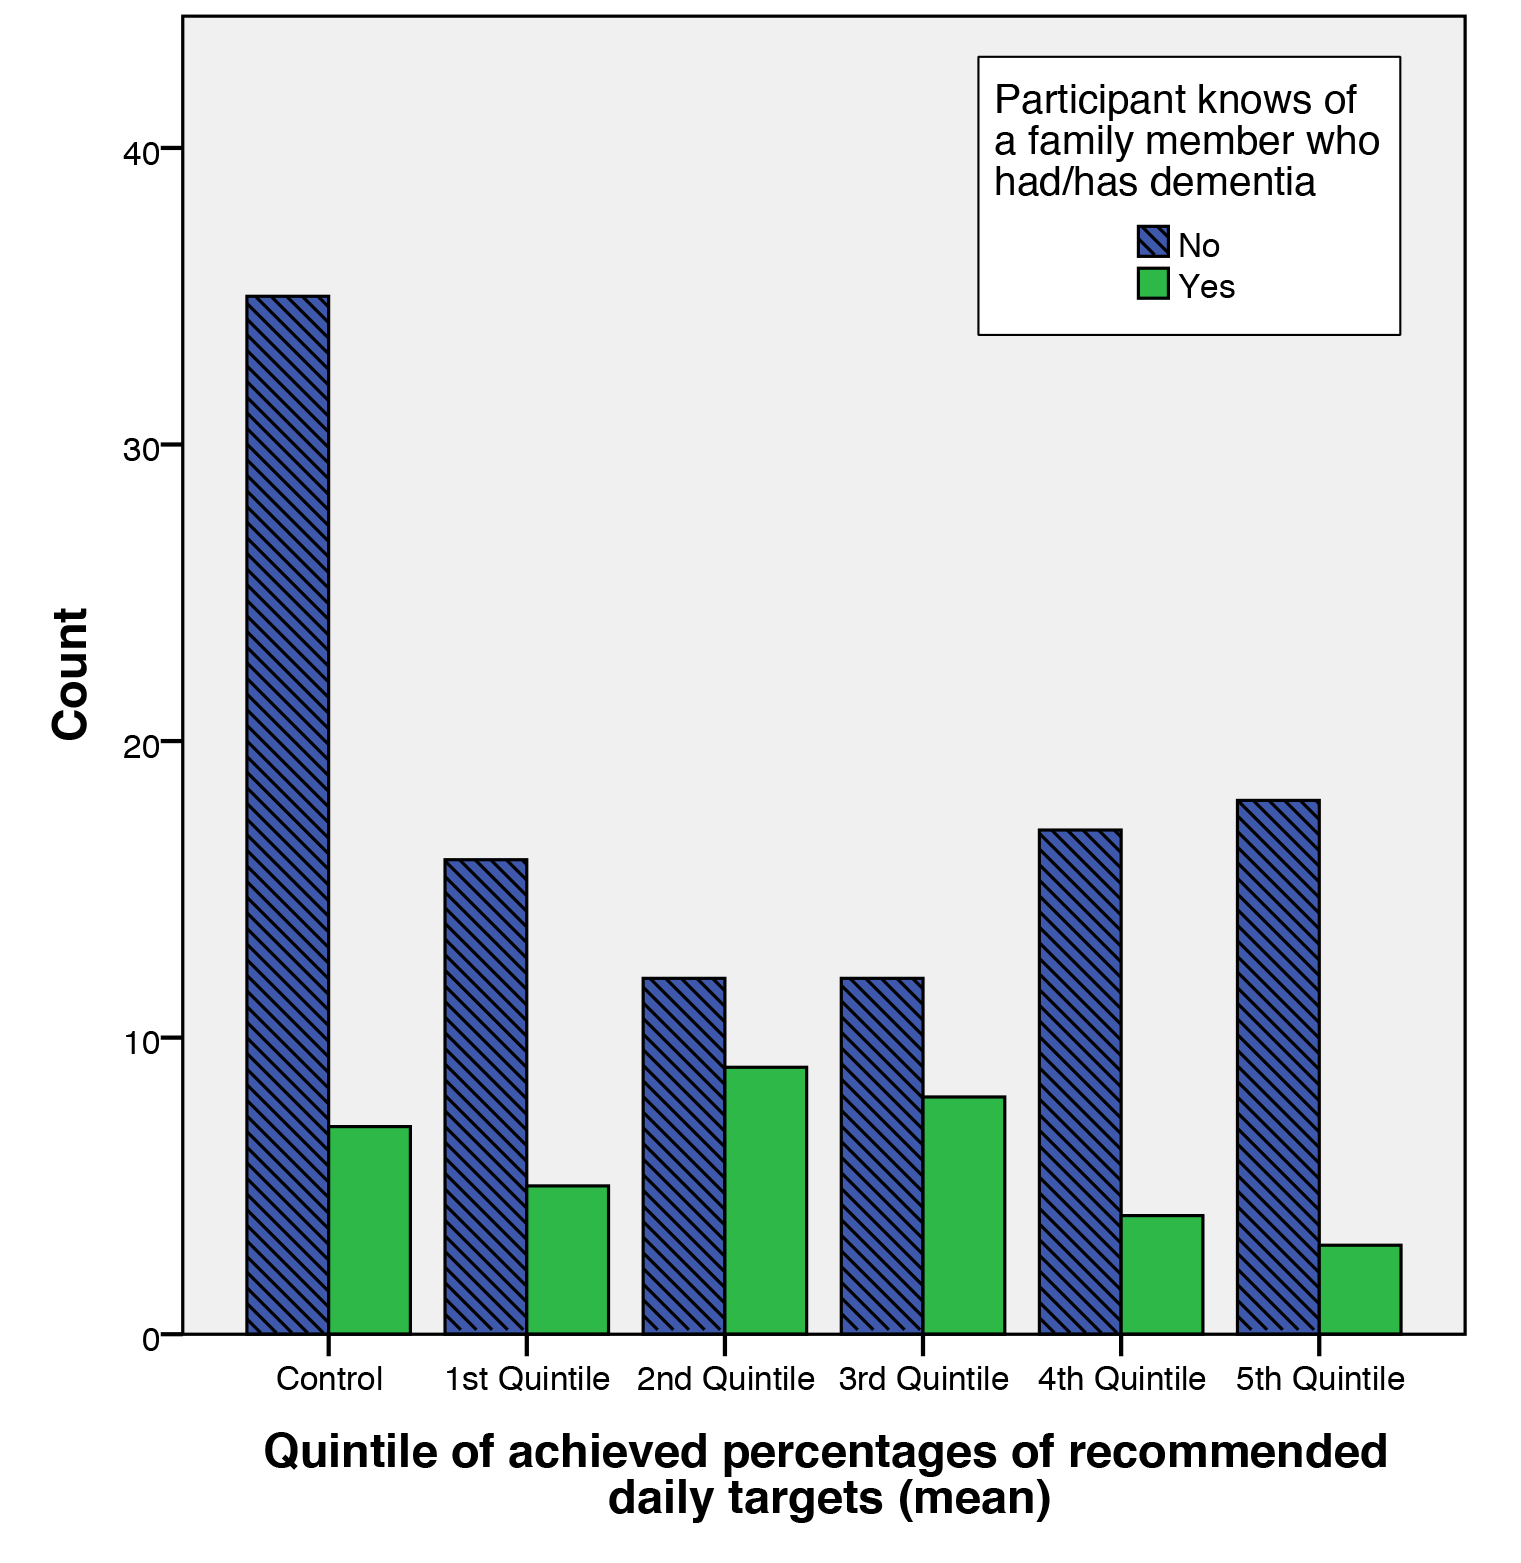
\includegraphics[scale=0.18, angle=0]{Files/prevention-study-3/figures/family-quintile}
  	\caption{Bar chart showing the performance quintiles and control group against the number of users who report to have known of a family member having/had dementia.}
    \label{fig: family-quintile}
\end{figure}

Research focused on the family members of persons with dementia has found that those who facilitate care typically suffer from higher rates of anxiety and depressive symptoms \cite{Mahoney2005} and as such may be increasingly motivated to reduce their own risk. This behaviour seems to appear in this RCT, as participants in the treatment group who have members of family with dementia and first-hand experience with the disease, are achieving a higher number of their recommended daily targets i.e. performing better within the realms of the study and theoretically reducing their AD risk.

\subsubsection{Gender}
Existing research has indicated that gender may play a role as to how AD risk is perceived or experienced \cite{Rose-Rego1998, Thompson2004}. As such the gender of participants and their achieved percentages were also analysed. Independent samples t-Test displayed that females achieved a statistically significant higher percentage of recommended targets (52.44 $\pm$ 29.24), compared to their male counterparts (38.69 $\pm$ 28.50), t(102) = -2.302, p = .023). In addition, analysis shows a visible correlation between gender and the ability to reach the recommended daily target values, as shown in Figure \ref{fig: gender-performance}. The reasons behind this particular observation are currently unclear and require additional analysis, however, could relate to motivations, occupation and education levels.

\begin{figure}[h]
	\centering
    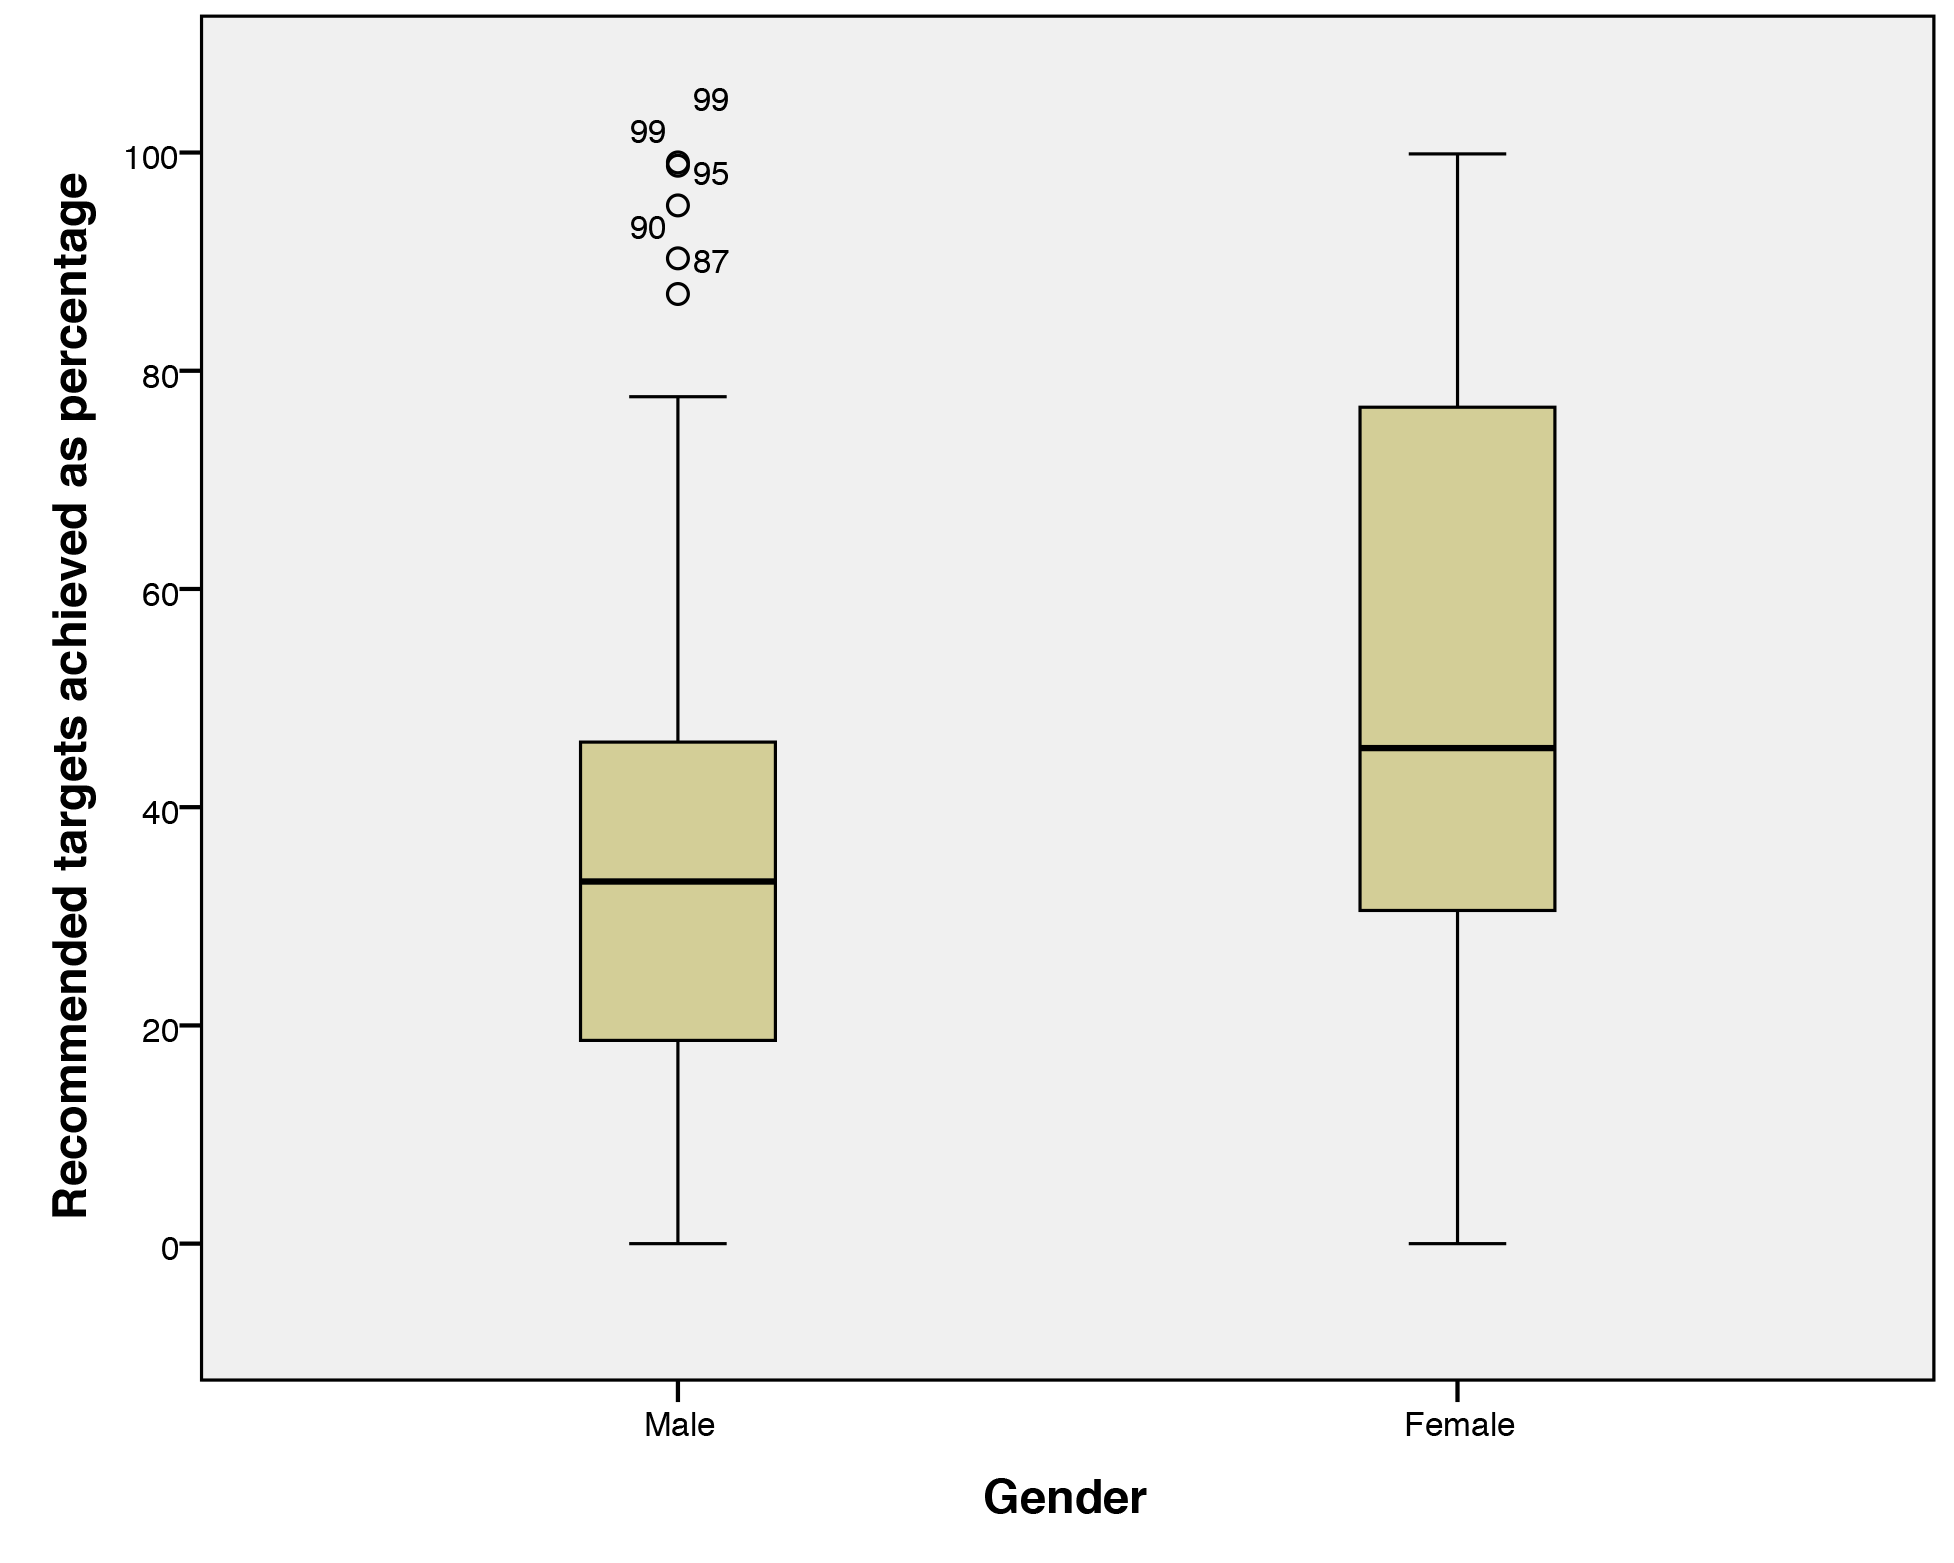
\includegraphics[scale=0.14, angle=0]{Files/prevention-study-3/figures/gender-performance.png}
  	\caption{Box-plot showing distributions of Male and Female mean percentages achieved targets across all domains.}
    \label{fig: gender-performance}
\end{figure}

\section{Principal Findings}
From the data generated within the RCT a number of results were found and have been categorised and presented, from a focal point of the smartphone app, as the principal findings of the study.

\subsection{Intervention delivery method}
The smartphone app provided a novel method to remotely monitor participants in a behaviour change intervention, whilst also facilitating the delivery of intervention material. The app had the ability to deliver multiple services through a single platform, and as a result was capable of facilitating stages 3-5 of the TTM, preparing participants for change, allowing them to accurately monitor and assess their actions and encouraging continued maintenance and improvement of their desired behaviours.
%VIVA: In the TTM these stages are procedural,  however,  the app offered them in parallel.  I am therefore not enitrley sure I agree with what you are saying here.
In addition, positive results from the exit-survey show that the majority of users wished to continue their behaviour change efforts, which were promoted by the app, and if maintained, are expected to yield superior outcomes in AD prevention.

\subsection{Importance of Goals and Recommended values}
In the RCT, the recommended values for each behaviour played a key role in both motivating the participant's to change their behaviours, and also as a metric for the uniform assessment of participant's performance. Analysis of pre-post measurements from the treatment group showed clear physiological changes in those who achieved the highest in their attempts to meet recommended values. This was especially apparent in those who were previously underachievers in certain behavioural domains, prior to the study (based on first week of observed behaviour logs). Effects observed included a desirable lowering of BMI, improvements in HDL and LDL cholesterols, improvements in systolic blood pressure, lowering of resting heart rate and improvements in perceived stress levels.

\subsection{Need for Personalised Data} \label{subsection: finding-need-personalised}
Regarding user experience, the majority of app users stated that they wished to alter their recommended values to be based on their ‘current’ health status, whilst others wish to manually set their own target goals. Such a feature was considered during the development of the app framework, however, was not implemented for this RCT to ensure that all participants received the exact same treatment and feedback.
In real-world scenarios personalised feedback and goal setting  could improve engagement with the app, especially for those who are underachieving significantly at the start of the treatment. A gradual increase of goals may be more apt for these individuals, with the ultimate goal of reaching or exceeding global recommendations based on the literature.
A suitable compromise for a controlled trial, may be to show both personalised \textbf{and} global targets, thus providing the same recommendations for all, but encouraging participants on an individual also.

\subsection{Targeted Behaviour Domains}
Around half of the respondents of the exit-survey stated that they wished  their educational material was focused on a specific domain of interest, rather than evenly spread throughout all behavioural domains. Such a focus may be beneficial if the user requires extensive change in one particular domain, however, for the purpose of a multi-domain intervention for an RCT the investigators decided it was of great importance to educate across all domains, supported by the literature of AD risk which is also multi-factorial \cite{Mangialasche2012}.

\section{Limitations}
The study does have limitations, namely that the RCT's findings may be bias to the cohort’s locale and ethnic group. The study cohort were predominantly white (96.6\%) and resided in an county that is classified as 96.23\% rural \cite{UnitedStatesCensusBureau}. Whilst desirable changes in behaviour were observed within this cohort, additional research is required to examine the efficacy of the approach within other countries, in various settings, spanning numerous ethnic groups.
Within a larger study, additional work would be required to accommodate and account for the cultural, regional and religious differences across groups, e.g. adjusting dietary recommendations based on religious practice.

\subsection{Healthy behaviours becoming unhealthy}
An additional limitation of the study was observed during the analysis of dietary behavioural data.
During the ranking of individuals based upon their ability to achieve recommended guidelines it became apparent that a number of participants who scored very highly in the dietary domain were categorised as Obese Class III (morbidly obese) in their BMI measurements. These individuals were regarded as overachievers, based upon the metric of target achieving, however, in the interests of health outcomes, the over-consumption of food has a negative side, even if the food consumed is deemed healthy.
For example, this study recommended the consumption of 1 serving of nuts daily, based upon the fact that nuts contain omega-3 fatty acids and vitamin-E, which are linked to improved cognition. A serving size of 1oz (21 kernels) of hazelnuts contains 178 calories. It is therefore easy to foresee that `over-achieving' in the consumption of healthy nuts, may also lead to undesired weight gain, and with it, additional health problems.
This raises the question \textit{at what point do healthy behaviours become unhealthy}, and how can a balance be found?
\newline It is perhaps therefore necessary to address this issue as an area for future improvement within the apps framework.

\section{Future Tech Improvements} \label{section: future-improvements}
Through analysis of data, survey analysis and direct communications with participants, various aspects of the app and supplementing technology have been identified for improvements.

\subsection{Wearable activity monitor selection}
The wearable activity monitors were donated by the Nike corporation for the study. Their activity monitor, the Nike+ Fuelband, uses the proprietary and non-disclosed metric of fuel points, which is rather ambiguous for the purpose of a scientific study. Many users reported that the device did not accurately reward them with points during activity, and conversely, awarded them with points when they were performing sedentary tasks, such as when they were driving their car. These false positives removed the opportunity to use the data to validate reported physical activity with the Nike Fuelband’s fuel point metric.

In agreement with the participant’s comments, a recent study assessing the validity of commercially available activity monitors found the Fuelband to be one of the weakest performers overall, undercounting daily step count, on average, by 2529 steps \cite{Ferguson2015}. There are now numerous commercially available alternatives, that allow for greater granularity in their data, such as step counts, distance travelled, sleep quality and resting heart rate. Many of these wearables allow for direct integration with apps via simple API calls. Due to this feature, self-reported sleep and physical activity may be correlated against the data collected directly from the wearable to examine validity. The future iteration plans to seek alternative wearable devices.

\subsection{Wearable integration}
As discussed earlier, the users also had the burden of repeatedly entering their fuel points via the log screen. This user burden of data entry can be greatly reduced by enabling the transfer of data from relevant wearable devices directly to the app, greatly increasing the convenience of the solution.

\subsection{Social Networking}
Participants had advised that they wished that the app were more socially engaging. This supports the findings from the previous Chapter, specifically the results displayed in Section \ref{subsection: social-integration} which showed that the integration of social elements result in a significantly higher MARS
score.
In addition, within the action phase (described in Section \ref{subsubsection: ttm-action-phase}) of the TTM, the helping relationships process requires the individual to be open and trusting with problems to someone else. As such, for future development, we have identified that a social element is required, allowing users to add friends with whom they can publicly share, and compare their efforts. Integrating the app with existing social networks, such as Facebook and Twitter, can facilitate this feature. Social network integration will allow the users to find friends already in their network, who are also using the app. From here they may compare their own accomplishments with those in their friend group, thus offering an opportunity to heighten motivations for change. In addition, integration with these networks will also allow users to post their accomplishments to their public pages, allowing those outside of the study to view their efforts and provide an opportunity for additional peer support, whilst boosting the public profile of the study.

\subsection{Improving Engagement}
Provided that the intervention material is sound, the main hurdle is engagement. The time of day analysis discussed in Section \ref{subsection: time-of-day}, and displayed in Figure \ref{fig: time-of-day}, highlights that it may be possible to use typical usage patterns to optimise the delivery of notifications, with the ultimate goal of improving engagement levels. Increased engagement would theoretically lead to greater levels of sustainable behaviour change.

\subsection{Personalisation} \label{subsection: gm-future-personalisation}
There is a huge opportunity for personalisation in all aspects of the app. As discussed in the principal findings (Section \ref{subsection: finding-need-personalised}), users of the app have suggested that they wish to set their own targets and behaviour change goals. This includes the addition or emphasis of particular domains based on a user’s own personal motivations. Daily fact delivery could also be revised to prioritise daily facts from a domain of interest to the user.

\subsection{Greater granularity}
Within the study, participants were asked to report behaviours which were reasoned as favourable by the investigators due to their role in AD prevention. As discussed in the limitations Section, this unexpectedly led, in some cases, to the overconsumption of foods which over-time could result in negative outcomes. When considering the diet domain, and all the behaviours that it entails, it became clear that the granularity of the data could be vastly improved. During the RCT, the participants were only asked to report desirable behaviours, however, did not track behaviours which should be avoided. For example, whilst participants were encouraged to consume fruits and vegetables, they were not asked to report how many refined sugars or processed foods they consumed. Using solely the measure of desirable food intake, without observing the undesirable food intake, resulted in a skewed representation of diet macronutrients and overall calories consumed.
As such, future versions of the app should also consider the tracking of negative behaviours, which will provide a much clearer picture of progress for both the participant, and study investigators.

\subsection{Additional Behavioural Domains (Smoking)}
Smoking cessation was not included in the original pilot study, as there is an extremely low rate of smokers in the Cache County area \cite{UtahDepartmentofHealth2014}. Nevertheless, if the Gray Matters study were to target a larger geographical area, state or nation-wide, facts and suggestions related to smoking cessation would be included.

\subsection{Improvement of Education Material}
With information on AD risk continually advancing, it is possible to continually strengthen and expand the daily fact database, adding new facts and suggestions, with each vetted using a modification of the rating system developed by the Grades of Recommendation, Assessment, Development and Evaluation (GRADE) workgroup \cite{Dijkers2013}. Analysis of in-app behaviours showed that users had tapped on questions numerous times to help them understand the exact semantics of a question. In addition, some external feedback outside of the study cohort suggested that some of the daily facts could have been clarified. As such, in future versions resources should be allocated to analyse the average user’s interpretation of daily facts and questions, to ensure that confusion is reduced.

\subsection{Distribution Method}
During the study, a number of suggestions were provided by users of the app informally via email. A familiar complaint was in relation to the use of the Testflight distribution platform. TestFlight, whilst useful for maintaining control of distribution, was developed for tech savvy users, not for clinical interventions. As such, many users had issues registering with the platform, subsequently approving certificates, and downloading the app. To avoid such complications, it is recommended that in future iterations, all distribution should take place via the platform’s official app repositories, iOS App Store and Google’s Play Store.
%VIVA: Chris - can you quantify the number of suggestions.


\subsection{User Interface}
With the ever changing UI guidelines of the iOS and Android platforms, any future version of the app will require elements of the UI to be updated. As the app was developed for the purpose of an RCT, the use of graphic design methodologies, including unique branding, colour, and typography, were low on the agenda. For greater adoption of the app, and increased user perception of efficacy, it is advised that the UI is highlighted as a primary task and designed to the highest-standard possible \cite{Soper2014}.

\subsection{Labelling data with tags}
During the analysis of behavioural data, the author realised that there was a limitation in the descriptive areas of the data. Specifically, there were moments in an individual's time-series data that an outlier was observed, for which no explanation could be derived from the data alone. These outlier values may have related to stress, or diet on a particular day.
To gain additional insight into each day, and to further explain outliers, the use of metadata tagging could be implemented. Social media websites commonly use hashtags, which serve as a type of tag which makes it easier for users to label their own content or find content with a specific theme.
\newline Within the app, a tag could be used to describe an experience, emotion, or activity that has happened that day. Examples include: \textbf{\#happy}, \textbf{\#sad}, \textbf{\#friends}, \textbf{\#gym}, \textbf{\#run}, \textbf{\#tired}, \textbf{\#sick} and so on. The user could select from a common list, and create their own. These tags would act as a type of diary, and a way for the user to label each day. Over time, days that were labelled with tags can be recalled and compared against one another. For example `Show diet for days labelled as \textbf{\#stress}'.
This would give a user greater understanding of their own behaviours and actions, whilst giving investigators a tremendous insight into how certain tags can alter behaviours, across numerous individuals.

\subsection{Rewards}
From the content analysis performed in Chapter \ref{chapter: prevention-evaluation}, it is apparent that gamification rewards may be given in numerous formats, including points, targets, achievements, and rankings. The Gray Matters app used in the RCT did not implement the full spectrum of available gamification reward types and as such has room for improvement in this area. The aforementioned rewards may be considered digital rewards, however, some companies are bringing these digital rewards into the physical domain. Strava is one such company. Within their platform users have the ability to obtain limited clothing items upon the achievement of certain challenges and milestones. Such a reward system is currently outside the scope of the Gray Matters app, however, it is important to recognise the evolution of reward systems in the digital domain.

\subsection{Ground Truth}
Despite the steps taken to ensure the data transmitted was valid, there are still weaknesses in the accuracy of the data reported. This is due to the data being generated through self-reporting, as opposed to direct observation. As such, there is no current ground truth data, from which to verify the user's reported behaviours. In this study it seems that participants were reasonably accurate in reporting their behaviours, due to the number of correlations found between behaviours and clinical measurements in numerous individuals. At a larger scale however, there is a need to ensure the data is as accurate as possible, and more than 1 source of information feed may be required.
One possible source of ground truth data for physical activity, stress levels and sleep quality may be from wearable devices. As stated before, the accuracy of wearable devices vary by each model and manufacturer. According to \citeauthor{Ferguson2015}, Withings and Fitbit devices showed the best accuracy compared to their ground truth data \cite{Ferguson2015}.

\section{Future Work}
Where the previous Section detailed future work for the technical improvement of the developed application, this Section discusses the additional analysis that could be performed given the wealth of data collected, however, but was outside of the research scope undertaken by the author.

\subsection{Intervention Components}
Further analysis can be performed to establish what effect, if any, the additional intervention components had on behavioural and clinical outcomes. For example, examining if the participants who used the personal coach had a difference in outcomes than those who did not.

\subsection{Targeted Domains}
At the beginning of the study participants were asked to identify the behavioural change domains that were of greatest interest to them. These domains were ranked from 1-6. It is therefore possible to analyse each participant's behaviour change in relation to their targeted domains. It may also be possible to examine the effect of the apps components in relation to specific domains. An untested hypothesis developed during the examination of future works, proposed that the app may be more suitable to aid change in certain behavioural domains than in others.

\subsection{Additional Booster Event Analysis}
Within the scope of the research, each booster events was analysed using ANOVA to assess its effect on behaviour change in a group of attendees. Often within these groups, 1 or more individuals had a significant difference in behaviours pre-post attendance, however, the significance of their individual changes was hidden when averaged across the group.
Analysing each attendee individually may lead to additional observations about the effects of booster events. Each participant who attended a booster event and experienced significant behavioural change afterward could be flagged for further study. Amongst these participants, there may be shared behavioural, clinical or demographic attributes which are yet to be explored, yet may lead to better use of intervention components in future or similar studies, and the ability to target them to specific user characteristics for optimal delivery.
%VIVA: Chris - You could also consider a MANOVA rather than ANOVA

\subsection{User Retainment}
Due to ethical reasons the participants who had access to the Gray Matters app during the intervention could continue to use the app after the study close. Despite the app receiving no active development, and being aware of this fact, many users continued to use the app and upload their behavioural logs to the servers. Data collected during this period was omitted from analysis, yet it may yield insights into user retainment and usage profiles. Further, it may give insight into those who used the app due to the Hawthorne effect \cite{McCarney2007}, and also highlight the characteristics of users who relied the most on the mobile intervention.

\section{Comments}
Despite encouraging results in the realms of academia, there is still considerably low public awareness of dementia risk, and the importance and relevance that modifiable lifestyle factors have on that risk \cite{FarrowM2008}. As \citeauthor{Deckers2015} state:
\begin{displayquote}
\textit{``This has important consequences: persons-at-risk do not seek help, they receive insufficient and inaccurate care and support from their social environment, and dementia is stigmatised.''} \cite{Deckers2015}
\end{displayquote}

As such, it is of importance that the general public become aware of the progressive research being undertaken, how technology can change their approach to living healthier, and the need for their input to develop future solutions.

\section{Impact in public domain after RCT}
Due to the relative success of the RCT in improving individual's behaviours related to AD risk, the study and app received public exposure through Alzheimer's research funding bodies, university affiliated press releases, newspapers, and social media outlets \cite{graymatterspress1,graymatterspress2,graymatterspress3,graymatterspress4}. With public interest peaking, there was an increased demand for the app to be made available to the public. Taking into consideration the improvements discussed in Section \ref{section: future-improvements}, a number of months were used to implement those which had the highest improvement-to-time ratio. The improvements included increasing the granularity of behavioural data and including the ability of users to track negative behaviours. Many of the questions which aimed to quantify behaviours via sentence based questioning were replaced with simple to use counters, which used colour to signify progress. For each behaviour and domain, progress could also be tracked on a daily, weekly and monthly basis, with progress against global and personal goals represented using a number of different graphic and visual formats.
In addition to these functional improvements, the app received a complete visual redesign, making it much more contemporary and in alignment with the app industry's call to align visuals with the recent `material design guidelines'. The app has been initially released as a beta for Android with the iPhone version currently in development at the time of writing this Thesis. Screenshots of the beta app are presented in Figure \ref{fig: graymatters-new}. In addition, a supplementery website\footnote{The Gray Matters app website available at: www.graymattersapp.org} was developed by the author to promote the app, aid dissemination of study findings and measure public interest using web-analytic packages. A screenshot of the homepage is presented in Figure \ref{fig: graymatters-online}.

\begin{figure}[h]
    \centering
    \begin{subfigure}[t]{0.3\textwidth}
        \centering
        
\includegraphics[width=\textwidth]{Files/prevention-study-3/figures/gm-new-tips}
        \caption{}
        \label{fig: gm-new-tips}
    \end{subfigure}
    \hfill
    \begin{subfigure}[t]{0.3\textwidth}
        \centering
        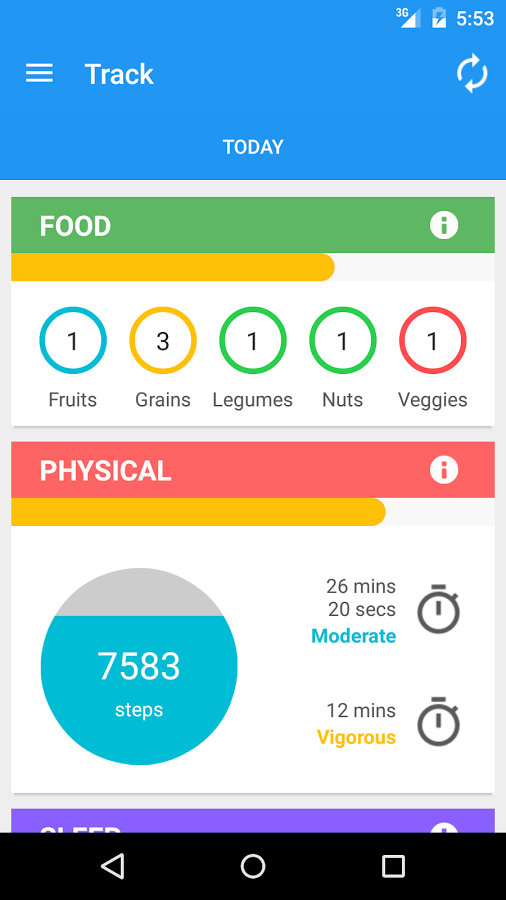
\includegraphics[width=\textwidth]{Files/prevention-study-3/figures/gm-new-log}
        \caption{}
        \label{fig: gm-new-log}
    \end{subfigure}
    \hfill
    \begin{subfigure}[t]{0.3\textwidth}
        \centering
        \includegraphics[width=\textwidth]{Files/prevention-study-3/figures/gm-new-performance}
        \caption{}
        \label{fig: gm-new-performance}
    \end{subfigure}
    \caption{Screenshots of redesigned Gray Matters app, released to public as beta release on the android OS. (A) Fact and suggestion presentation. (B) Behavioural logging with real-time progress indicators. (C) Showing current progress against their average performance.}
    \label{fig: graymatters-new}
\end{figure}

\begin{figure}[h]
    \centering
    \begin{subfigure}[t]{0.48\textwidth}
        \centering
        \includegraphics[width=\textwidth]{Files/prevention-study-3/figures/graymatters-web}
        \caption{}
        \label{fig: gm-web}
    \end{subfigure}
    \hfill
    \begin{subfigure}[t]{0.48\textwidth}
        \centering
        \includegraphics[width=\textwidth]{Files/prevention-study-3/figures/graymatters-playstore}
        \caption{}
        \label{fig: gm-playstore}
    \end{subfigure}
    \caption{Screenshots of public website and Google Play store listing. (A) www.graymattersapp.org. (B) Google Play store listing.}
    \label{fig: graymatters-online}
\end{figure}

The beta release was initially aimed to generate interest within the research and clinical domains, to encourage the creation of an intellectual consortium related to the works. Nevertheless, many of those in the public domain were inspired by the media exposure and created a demand for access to the app as soon as possible, and subsequently it was made available as a free beta on the android play store.

\section{Closing Remarks}
This demand from the public emphasises the apparent need for a solution, especially from those who wish to take their overall health, including AD risk, into their own hands. It can be argued, as is often the case with new technology, that the most technologically capable will be those to benefit from it, and the rest of society will take years to adopt, or miss out completely. Unlike technology platforms of the past, however, smartphones are now truly ubiquitous across all levels of society. With this in mind, and the increasing scientific literature supporting behaviour change and future disease risk increasing, it will not be long until it is the social norm for individuals to actively seek out personalised preventative medicine for specific diseases, and use an app to guide them on their quest for behaviour change.

With such a future envisaged, the previous 3 Chapters have contributed to knowledge in the area by detailing a procedural framework to develop behaviour change apps, documented by the development of an app by applying the framework, evaluated the resulting app with domain experts, and presented the clinical and behavioural results from a 6-month RCT using the app as an  intervention.
 % 6 GM Study & Results
\chap{Conclusion and Future Work}
\label{chapter: conclusion}

This chapter concludes and summarises the results from thesis studies, summarising the findings and producing a number of messages for various research fields and practices.

\section{Thesis Summary}
Through this body of work the underlying theme has been to exploit the ubiquitous nature of smartphones to improve in health and wellbeing outcomes. This has been demonstrated in two distinct cases studies which span both the treatment and prevention areas of Alzheimer's disease. 

Chapter \ref{chapter: treatment-framework} focused on using the ever available smartphone as the platform for an assistive reminder tool for persons with dementia. The adoption of the solution from the cohort was encouraging, yet over-time exposed fundamental issues regarding technology adoption with the elderly and cognitively impaired. Despite a lack of widespread adoption at the end of the 12 months, the data from the study permitted the concept of using smartphone sensors to predict if a reminder will be acknowledged or missed, to be proven. The following question, yet to be answered, is if this will improve the acknowledgement rates of reminders, and if that will consequently result in improved adherence to the actual tasks being reminded. As such, the models described in the chapter need be implemented and evaluated with another, comparable, cohort.

Chapters \ref{chapter: prevention-framework}, \ref{chapter: prevention-evaluation}, \ref{chapter: prevention-rctresults} were focused heavily in the areas of dementia prevention through behaviour change, facilitated by a smartphone app. The works demonstrated how disease risk could be mitigated by applying a process framework developed by the author, to a disease area. The result of which produces an app which guides and encourages users, step by step, to change disease associated behaviours, resulting in continual health improvement. Unlike the work in chapter \ref{chapter: treatment-framework}, the study participants had no such percieved barriers to adoption, and as such the case study truly exploited the pervasive nature of the smartphone, yielding every advantage offered to integrate with an individual’s daily life and routines. 
 
\subsection{Contributions to Knowledge}
\begin{itemize}
	\item Demonstrated use of sensor data to infer opportune moments to deliver reminders, for PwD and healthy individuals.
	\item Developed mobile-app behavioural change framework and guidelines.
	\item Detailed impartial approach to critically evaluate and rate mHealth apps.
	\item Demonstrated behavioural effects of applied framework.
	\item Demonstrated clinical efficacy of applied framework.
	\item Identified areas for future mHealth-supported behavioural research.
	\item Identified areas for future research of reminder tools for PwD.
\end{itemize}

\subsection{Future Work}
Throughout the works, during reviews of existing literature, analysis of study data, and interviews with study participants, a number of areas were identified by the author in which future study could improve, or elicit new and interesting, findings.

\subsubsection{Advanced Personalisation and Feedback}
Interviews and questionnaires performed by the participants in the Gray Matters study indicated that \textit{truly}personalised feedback was greatly desired. Specifically, participants wanted to see personalised progress reports, based upon their own efforts, rather than those imposed by global recommendations. Whilst the study collaborators had foreseen this, it was agreed that it would detract from assessing motivation for established goals. In retrospect however, it may have been possible to facilitate both, as discussed in Section \ref{subsection: gm-future-personalisation}. As the demand for such a feature was so high, it is anticipated that personalised goal setting may significantly increase both adoption and user retention, two key factors for successful behaviour change.

\subsubsection{Artificial Intelligence Coaching}
In the Gray Matters study, participants had reported that there were various times when a fact and suggestion pair was not fully understood, or had raised additional personal queries, for which the app had no answers. Often the participants would turn try to reach out to the study investigators, in some cases eventually turning to online search websites for answers. The queries were simple, and typically related to diet and exercise. An example scenario:
Daily suggestion presents: 'Eat 2 cups of brown rice instead of chips with dinner tonight'. User would like to know if white rice is Ok, as they do not own brown rice. 
It is a simple query, and the answer is relatively inconsequential, however, a lack of answers extrapolated over numerous users and time, will result in loss of users, and thus loss of impact. A human operated query answering facility to service a large user based is also not feasible. However, great progress is currently being made in natural language engineering, enabling the ability to answer open questions through databases of expert knowledge \cite{HIRSCHMAN2001, Fader2014}. Application of these techniques, whilst advanced, will allow researchers to develop a deeper suggestion base, and provide a much higher level of support to end-users.
 
\subsubsection{Evaluation of sensorised reminder delivery system}
The work performed in Chapter \ref{chapter: treatment-framework} needs to be extended to fully achieve the original goal of improving adherence to reminders for PwD. The current work provides a solid technological base from which the models may be implemented on a smartphone, or cloud. The app was written in a modular approach, with the intension to be extended by the author and others in the field. Currently, the base application has been extended by \citeauthor{Patterson2015} who aims to use the platform to assess and eventually improve task completion followthrough, once a reminder has been issued \cite{Patterson2015}.

\subsubsection{Carer-focused Apps}
Carers of PwD are often family members, whose age would be similar as the middle-aged cohort in the Gray Matters study, who posed very minimal barriers to successful technology adoption. Given the opportunity to expand upon the work performed in Chapter \ref{chapter: treatment-framework} the author would desire to create a carer orientated solution, removing the need for the PwD to have any interaction with technology.

\section{Messages for Behavioural Scientists}
\textbf{Harness the Smartphone.}
Changing behaviours may be the key to tackling the leading causes of mortality and morbidity, such as poor diet choices, lack of exercise, smoking and alcohol consumption. Diet and exercise apps to quantify efforts do exist, some with their foundations in exercise and nutritional science, yet there is a gaping void where behavioural and psychological science based apps should be. 
The smartphone, like no other tool before it, has become part of everyday life, embedded into the behaviours of millions, giving direct access to quantifiable data. Through the understanding of behaviours on a global scale, the development of all health interventions will improve. It is of the authors opinion, that the merging of behavioural science with ubiquitous computing, currently in the form of smartphones, stands to empower the individual, and revolutionise healthcare on a global scale. 

\section{Message for Technologists}
\textbf{Technology is the question, not the answer.}
Whilst technology may hold some of the answers, it is not \textit{the} answer. Before applying technology to a problem area, ask, \textit{does it really belong there?}
A great level of diligent research must be performed, drawing knowledge from every available perspective, through collaboration and interdisciplinary research. Whilst it is true that technology-led health-orientated projects often advance the state-of-the-art, it seems seldom that they actually prove efficacy over more traditional, non-technology based approaches. With increased focus on efficacy and impact, funding and reputations are at stake. It is up to us, the technologists, to prove that the field deserves the spotlight that it gets, through true collaboration, not discordant co-operation. % 7 Conclusion

%% Appendices -----------------------------------------------------
\addtocontents{toc}{\vspace{2em}} % Add a gap in the Contents, for aesthetics
\lhead{\emph{Appendices}}  % Change the left side page header to "Appendices"
\appendix % Cue to tell LaTeX that the following 'chapters' are Appendices

\chap{Domain Tips} \label{apndx: domain-tips}
This appendix details the tips and further information for each behavioural domain provided to users of the Gray Matters app. The data is categorised under its' respective domain.

\section{Diet}
\textbf{Healthy food choices feed the brain and lower risk for Alzheimer's disease.}
Just like the rest of your body, your brain needs a nutritious diet to operate at its best. \textit{Focus on eating plenty of fresh fruit and vegetables, lean protein, and healthy fats.}
Eating habits that reduce inflammation and provide a steady supply of fuel are best. These food tips will keep you protected:
\newline \textbf{Follow a Mediterranean diet.}
Eating a heart-healthy Mediterranean diet rich in fish, nuts, whole grains, olive oil, and abundant fresh produce. You can treat yourself to the occasional square of dark chocolate, and if you consume alcohol, a glass of red wine.
\newline \textbf{Avoid trans fats and saturated fats.}
Reduce your consumption by avoiding full-fat dairy products, red meat, fast food, fried foods, and packaged and processed foods.
\newline \textbf{Eat a heart-healthy diet.}
What's good for the heart is also good for the brain, so by reducing your risk of heart disease, you also lower your risk of Alzheimer's disease.
\newline \textbf{Get plenty of omega-3 fats.}
Evidence suggests that omega-3 fatty acids may help prevent Alzheimer's disease and dementia. Food sources include cold-water fish such as salmon, tuna, trout, mackerel, and sardines. You can also supplement with fish oil.
\newline \textbf{Eat across the rainbow.}
Emphasize fruits and vegetables across the color spectrum to maximize protective antioxidants and vitamins. Daily servings of berries and green leafy vegetables should be part of your brain-protective regimen.

\section{Physical}
\textbf{Research shows that people who exercise regularly have a lower risk for multiple degenerative diseases, including Alzheimer's.}

\textit{Quality and quantity} of the physical activity are important. 

Incorporating physical activity into your daily routine is linked to:
\begin{enumerate}
	\item Lower stress levels
	\item Better physical health
	\item Improved sleep
	\item Enhanced brain performance
\end{enumerate}

\section{Sleep}
\textbf{Good sleep is linked to better mental performance during the day, and lower risk for Alzheimer's disease.}

Promote better sleep by:  
\begin{enumerate}
	\item \textit{Avoiding caffeine} within 4 hours of bedtime 
	\item Finishing exercise \textit{3 hours or more} before bedtime 
	\item Creating a \textit{quiet and dark} environment
	\item Maintaining a \textit{regular bedtime} and wake-up time each day, to help set your internal 'clock' for better sleep.
\end{enumerate}

\section{Social}
\textbf{Research shows that people who have a socially engaged lifestyle, have \textit{higher scores on cognitive tests}, and are at a \textit{lower risk for dementia} and Alzheimer's disease.}

\textit{Quality is more important than quantity}

Feeling emotionally supported and having low conflict with others is linked to:
\begin{itemize}
  \item Lower stress
  \item Better physical health
  \item Better brain performance
\end{itemize}

\section{Cognitive}
\textbf{Stimulating your brain by mentally challenging yourself builds \textit{'cognitive reserve'}, associated with lower Alzheimer's risk.}

\textbf{Novel mental exercises} are very important (e.g. memorizing a recipe or grocery list, learning new words or a foreign language, doing arithmetic problems, helping kids/grandkids with homework). 

Also important are \textbf{cognitively stimulating activities}, things like volunteering, joining a book club, playing a musical instrument, attending a lecture or concert, or debating friends on the hot topic of the day! 

Keep it fun so you'll stick with it!"

\section{Stress}
\textbf{Psychological stress increases risk for Alzheimer's disease.}

Lower your AD risk by taking a moment to \textit{manage your daily stressors} and building into each day a time to reflect and be mindful of what is truly most important in life. 

Try doing this by \textit{increasing awareness }of your mind and body and allowing yourself to take a break from the stress. 

\textit{Taking a walk, talking to a friend, or contacting a loved one} can provide the opportunity to be both aware and a time-out to reset your stress.

\section{Extra: Drinks}
\texttt{This section was not included in the original RCT study version of the Gray Matters app, however, was developed for the second iteration released to the public.}

\textbf{The human brain is composed of 95\% water, blood is 82\% water, and the lungs are nearly 90\% water}

\textbf{How important is water to us?}
\newline A 2\% drop in body water can cause a \textit{small but critical shrinkage of the brain}, which can impair neuromuscular coordination, decrease concentration, and slow thinking. 

Dehydration can also reduce endurance, decrease strength, cause cramping, and slow muscular response.

It is suggested that the average person requires a \textbf{\textit{minimum of 8-to-12 glasses of water per day}}. If you are doing exercise, in a hot climate, or consuming alcohol, make sure to add a few extra glasses!
 % Prevention appendix
\chap{MARS Pilot Re-evaluation} \label{apndx: mars-pilot-reevaluation}

\begin{sidewaystable*}
	\centering
\caption{Testing for Disciplinary Bias - Full assessment results}
\label{my-label}
\resizebox{\textwidth}{!}{%
\begin{tabular}{@{}llllllllllllllllllllllll@{}}
\toprule
 & \multicolumn{5}{c}{Engagement} & \multicolumn{4}{c}{Functionality} & \multicolumn{3}{c}{Aesthetics} & \multicolumn{7}{c}{Information} & \multicolumn{4}{c}{Subjective} \\ \midrule
App & Entertainment & Interest & Customisation & Interactivity & Target Group & Performance & Ease of Use & Navigation & Gestural Design & Layout & Graphics & Visual Appeal & Matches description & Goals & Quality & Quantity & Visual & Credibility & Evidence-base & Recommend? & How often would use? & Pay? & Overall Rating \\ \midrule
Breathe Daily & 4 & 3 & 3 & 5 & 4 & 4 & 5 & 4 & 4 & 4 & 3 & 3 & 4 & 5 & 3 &  & 4 & 2 &  & 2 & 2 & 1 & 2 \\
Everyday Health with Acupressure & 4 & 3 & 3 & 3 & 3 & 4 & 4 & 4 & 4 & 4 & 4 & 4 & 4 & 3 & 3 & 4 & 4 & 2 &  & 2 & 4 & 3 & 4 \\
Interpersonal Dynamics & 4 & 4 & 3 & 3 & 4 & 4 & 4 & 4 & 4 & 4 & 4 & 4 & 4 & 3 & 5 & 4 & 4 & 4 &  & 4 & 3 & 3 & 4 \\
iPhoria Nature’s Music & 4 & 4 & 3 & 4 & 3 & 5 & 5 & 4 & 4 & 4 & 3 & 2 & 4 &  &  &  &  & 2 &  & 2 & 1 & 1 & 2 \\
iThoughtjournal & 3 & 4 & 5 & 4 & 5 & 4 & 5 & 5 & 4 & 3 & 2 & 2 & 4 &  &  &  &  & 2 &  & 4 & 4 & 1 & 3 \\
Meditation Seconds Lite & 4 & 4 & 3 & 3 & 4 & 4 & 5 & 4 & 4 & 3 & 4 & 3 & 4 &  & 3 & 2 &  & 2 &  & 1 & 2 & 1 & 2 \\
Personal Remedies & 3 & 4 & 3 & 3 & 3 & 4 & 4 & 4 & 4 & 4 & 3 & 4 & 4 &  & 4 & 4 &  & 2 &  & 3 & 3 & 3 & 3 \\
Sleep Easily & 3 & 4 & 3 & 3 & 4 & 4 & 5 & 4 & 4 & 5 & 4 & 4 & 4 &  & 4 & 3 &  & 2 &  & 3 & 3 & 3 & 3 \\
We Breathe & 3 & 4 & 3 & 4 & 4 & 4 & 5 & 4 & 4 & 4 & 4 & 3 & 4 & 4 & 3 & 4 & 4 & 2 &  & 4 & 3 & 1 & 3 \\ \bottomrule
\end{tabular}
}
\end{sidewaystable*} % Prevention appendix

%% Bibliography 
\backmatter % Cue to tell LaTeX that the following 'chapters' are Bibliography
\label{Bibliography}
\lhead{\emph{Bibliography}}  % left side page header to "Bibliography"

\begingroup
\raggedright
\sloppy
\printbibliography
\endgroup
\end{document}